\documentclass[
    a4paper,
    brazil,
    12pt,
        ]{icmc}

%\voffset=0pt
%\usepackage[none]{hyphenat}	para evitar hifenizacao
\hyphenpenalty=2000 		% (nao ta funcionando)
\tolerance=400			%
\clubpenalty=10000		% Alteração Vinícius
\widowpenalty=10000		%
\displaywidowpenalty=10000	%

% alteracao Vinícius
%\usepackage{tocloft}

%\newlength\mylena
%\settowidth\mylena{Figura}
%\newlength\mylenb
%\settowidth\mylenb{Tabela}

%\addtolength\cftfignumwidth{\mylena}
%\addtolength\cfttabnumwidth{\mylenb}

%\renewcommand\cftfigpresnum{Figura }
%\renewcommand\cfttabpresnum{Tabela }
%fim
%
\usepackage{listings,listings}
\usepackage{array}
\usepackage{graphicx}
\usepackage{hyperref}
\usepackage{scalefnt}
%************************


%\usepackage{amsmath}
%\numberwithin{equation}{section}
%\usepackage{amssymb}
\usepackage{multicol}

\usepackage{graphicx} 
%5\usepackage{subfig}
\usepackage{scalefnt}
\usepackage{lscape}
\usepackage{longtable}
\usepackage{multirow}
%\usepackage{tabularx}
\usepackage{color}
%*********************
\usepackage{pdfpages}
\usepackage[brazil]{babel}


%Landir -------------------------------------------
\usepackage{multirow}
\newcommand{\conj}[4]{#1=\{#3~|~#2 \leq #3 \leq #4, ~#3 \in \mathbb{N}\}}
\newcommand{\matrizz}[7]{#1_{#2 \times #3} \textrm{, } #4_{#5 #6} \in \mathbb{#7}}
\newcommand{\matrizzz}[9]{#1_{#2 \times #3 \times #4} \textrm{, } #5_{#6 #7 #8} \in \mathbb{#9}}
\newcommand{\interval}[3]{#1 \leq #2 \leq #3}
\newcommand{\quintupla}[5]{\langle #1,#2,#3,#4,#5 \rangle}
\newcommand{\tripla}[3]{\langle #1,#2,#3 \rangle}
\newcommand{\parord}[2]{\langle #1,#2 \rangle}

%ambiente para definições, teoremas etc...
\newtheorem{defi}{Definição}[chapter]
\newtheorem{propri}{Propriedade}[chapter]
\newtheorem{conce}{Conceito}[chapter]
\newtheorem{propo}{Proposição}[chapter]
\newcommand{\dsum}{\displaystyle\sum}
\usepackage{algorithm}
\usepackage{clrscode3e}
\usepackage{lscape}	%pagina em formato paisagem
%--------------------------------------------------

\usepackage[toc,page]{appendix}
\usepackage{isoaccent}
\usepackage{setspace}
\usepackage{babel}
\usepackage{float}
\usepackage{longtable}
\usepackage[nottoc]{tocbibind}
\usepackage{graphicx}
\usepackage{epstopdf}
%--------------------------------------------------
\usepackage{subfigure}
\graphicspath{{figuras/}}

%--------------------------------------------------

\usepackage{amssymb, amsmath}
%% --------------------------------------------------------------
%% se for quali, substitua "capaUEM" por "capaUEMquali" 
\usepackage{capaUEM}      % Para formatação de capa e folhas de rosto
%%
%% ---------------------------------------------------------------
\usepackage[
    sort&compress,
    %numbers,
    authoryear,
    ]{natbib} % Para usar estilo novo de referências
\usepackage{verbatim}
\usepackage{titlesec}
\usepackage{enumerate}
\usepackage{pdfpages}
\usepackage{colortbl}
\usepackage{color}
\usepackage{textfit}
\usepackage{tabularx}
\usepackage{rotating}
\usepackage{fancyhdr}
\usepackage{url}
\usepackage{placeins}
\usepackage{afterpage}
\usepackage{setspace}
\usepackage{amsmath}
%\singlespacing
\onehalfspacing
%\doublespacing
%\setstretch{1.1}

\RequirePackage{ifthen}
%
% Importando APUD do abntcite.sty
%
\newcommand{\apudname}{apud}
\def\citeopen{(}
\def\citeclose{)}

\newcommand{\apud}[3][]{\citeopen\citeauthor{#2}, \citeyear{#2} \apudname\ %
\citeauthor{#3}, \citeyear{#3}%
\ifthenelse{\equal{#1}{\empty}}{}{, #1}\citeclose}

\let\cite=\citep    % O natbib requer \citep para referências. Então, se vc já escreveu muita coisa usando \cite, este comando substitui na hora de compilar

\usepackage[a4paper, top=3cm, bottom=2cm, %   footskip=15pt,
    verbose,
    left=3cm,
    right=2cm,
  ]{geometry}

%\widowpenalty=350 % comentado por Vinicius
%\clubpenalty=350  % ''

\exhyphenpenalty=10000 \hyphenpenalty=800

\vfuzz1pc % Don't bother to report overfull boxes if over-edge is < 1pc
\hfuzz1pc % Don't bother to report overfull boxes if over-edge is < 1pc

\newcommand{\atributo}[1]{\textbf{\textit{#1}}}


%% Limpa os cabeçalhos, deixando só o número da página
\renewcommand{\headrulewidth}{0pt}
\pagestyle{fancyplain}
\fancyhf{}
\rhead{\fancyplain{}{\thepage}}

%% Muda a formataçao dos títulos das listas de figuras, tabelas e sumário
\makeatletter

\def\tableofcontents{
\newpage
\pagestyle{empty}
\centerline{\large \textbf{SUMÁRIO}}
\@mkboth{SUMÁRIO}{SUMÁRIO}
\@starttoc{toc}
}

\def\listoffigures{
\newpage
\pagestyle{empty}
\centerline{\large LISTA DE FIGURAS}
\@mkboth{LISTA DE FIGURAS}{LISTA DE FIGURAS}
\@starttoc{lof}
}



\def\listoftables{
\newpage
\pagestyle{empty}
\centerline{\large LISTA DE TABELAS}
\@mkboth{LISTA DE TABELAS}{LISTA DE TABELAS}
\@starttoc{lot}
}
\makeatother
\hyphenation{proba-bi-li-da-des}
\hyphenation{apre-sen-tar}
\hyphenation{gra-ma-ti-cais}
\hyphenation{e-qui-va-le}
\hyphenation{es-ta-be-le-ci-das}
\hyphenation{cate-goria}

%%%%%%%%%%%%%%%%%%%%%%%%%%%%%%%%%%%%%%%%%%%%%%%%%%%%%%%%%%%%%%%%%%%%%%%%%%%%%%%%%%%%%%%%%%%%%%%%%%%
% Estilos diferentes para cabeçalho de capítulo - by Adenilso
%%%%%%%%%%%%%%%%%%%%%%%%%%%%%%%%%%%%%%%%%%%%%%%%%%%%%%%%%%%%%%%%%%%%%%%%%%%%%%%%%%%%%%%%%%%%%%%%%%%

\makeatletter  %usado para que o @ seja considerado
 \newcounter{capkind}
 \setcounter{capkind}{1}   % define qual tipo de cabeçalho usar
    
     
 \ifcase\value{capkind}
 \def\@makechapterhead#1{%
 \begingroup
 \centering
   \vspace*{50\p@}%
         \noindent\begin{tabular}{p{0.34\textwidth}|p{0.22\textwidth}|p{0.34\textwidth}}
   \cline{2-2}
   \raisebox{0pt}[25pt][15pt]{}& \centering\large{\sffamily\scshape{\@chapapp}}\space \itshape\thechapter & \\
   \hline
   \hline
       \multicolumn{3}{|p{0.97\textwidth}|}{\raisebox{0pt}[30pt][20pt]{}\centering\Huge \bfseries #1}\\
   \hline
   \hline
   \raisebox{0pt}[10pt][10pt]{}&  & \\	
   \cline{2-2}
   \end{tabular}\par
   \vspace*{40\p@}%
 \endgroup
 }
 \def\@makeschapterhead#1{%
 \begingroup
 \centering
   \vspace*{50\p@}%
         \noindent\begin{tabular}{p{0.34\textwidth}|p{0.22\textwidth}|p{0.34\textwidth}}
   \cline{2-2}
   \raisebox{0pt}[10pt][10pt]{}&  & \\
   \hline
   \hline
       \multicolumn{3}{|p{0.97\textwidth}|}{\raisebox{0pt}[30pt][20pt]{}\centering\Huge \bfseries #1}\\
   \hline
   \hline
   \raisebox{0pt}[10pt][10pt]{}&  & \\	
   \cline{2-2}
   \end{tabular}\par
   \vspace*{40\p@}%
 \endgroup
 }
 \or %%%%%%%%%%%%%%%%%%%%%%%
 
 \def\@makechapterhead#1{%
 \begingroup
   \vspace*{50\p@}%
      \noindent
       \sffamily\Huge\hrulefill          
      {\begin{tabular}{|c|}
          %\rowcolor{black}
          \hline
          \color{white} \large \scshape % \@chapapp{} \\
          %\hline
          \vspace{-2ex}\\ %coloquei para aumentar o espaço entre o título e o número
          \Huge \slshape \scaletoheight{1cm}{\thechapter} \\ \hline
      \end{tabular}     
      }
   
      \par
      \vspace*{18\p@}
      {\Huge\bfseries\begin{flushright} #1\end{flushright}}\par
      \vspace*{-6\p@}
      \hspace*{0pt plus 1fill}
     	\rule{.8\textwidth}{0.5pt}\\[-36\p@]
     \hspace*{0pt plus 1fill}
      \rule{.8\textwidth}{3pt}
      \vskip 1.7ex
 \endgroup
     }
                               
 \def\@makeschapterhead#1{%       Essa parte configura o cabeçalho do capítulo referências
  
 \begingroup
   \vspace*{30\p@}%
      \noindent
      \sffamily\Huge
      {\Huge\bfseries \begin{flushright} #1\end{flushright}}\par
      \vspace*{0\p@}
 %     \hspace*{0pt plus 1fill}
 %     	\rule{.8\textwidth}{0.5pt}\par
      \vspace*{-12\p@}
      \hspace*{0pt plus 1fill}
       \rule{.8\textwidth}{3pt}
      \vskip 1.7ex
      
 \endgroup
      
   
     }
     \def\@schap#1{%      
  	 \begingroup
   \vspace*{30\p@}%
      \noindent
      \sffamily\Huge
      {\Huge\bfseries \begin{flushright} #1\end{flushright}}\par
      \vspace*{0\p@}
 %     \hspace*{0pt plus 1fill}
 %     	\rule{.8\textwidth}{0.5pt}\par
      \vspace*{-12\p@}
      \hspace*{0pt plus 1fill}
       \rule{.8\textwidth}{3pt}
      \vskip 1.7ex
      
 \endgroup
      
   
     }

  


\fi

\makeatother %para voltar a ignorar o @
%\includeonly{gerenciamento}
\begin{document}

%%%%%%%%%%%%%%%%%%%%%%%%%%%%%%%%%%%%%%%%%%%%%%%%%%%%%%%%%%%%%%%%%%%%%%%%%%%%%%%%%%%%%%%%%%%%%%%%%%%
%% DADOS PARA CAPA, FOLHA DE ROSTO E FOLHA DE APROVAÇÃO

% Dados autor
\Jautor{KLEBER LOPES PETRY}

% Dados trabalho: título e subtítulo (opcional)
\Jtitulo{SMartyTesting: Uma Abordagem de Teste Baseado em Modelos
	SMarty para Linha de Produto de Software}
%\Jsubtitulo{: uma nova solução ...} %% descomente essa linha caso haja um subtítulo
\Jtituloabs{SMartyTesting: An SMarty Model-Based Testing Approach for Software Product Line}
%\Jsubtituloabs{: a new solution...} %% descomente essa linha caso haja um subtítulo

% Ano da defesa
\Jdata{2019}

% Dados orientação
\Jtipoorientador{o} %% caso seja orientador
\Jorientador{Edson A. Oliveira Junior}
\JtipobancaC{o} %% caso seja professor (usado na folha de aprovação)

%\Jcoorientador{o}{Jose} %% caso não haja coorientador(a) comente esta linha e a próxima
%\Jtipocoorientador{o} %% caso seja coorientador
%\Jtipocoorientador{a} %% caso seja coorientadora
%\JtipobancaC{a}  %% caso seja professora (usado na folha de aprovação)

% Dados da banca
%\JtipobancaA{a} %% caso seja professora
\JtipobancaA{o}  %% caso seja professor
\JbancaA{Fulano 1}
\JinstituicaoA{Universidade Estadual de Maringá --- DIN/UEM}

%\JtipobancaB{a}  %% caso seja professora
\JtipobancaB{o} %% caso seja professor
\JbancaB{Fulano 2}
\JinstituicaoB{Universidade Federal do Fim do Mundo --- DEINFO/UFFM}

% Dados da defesa
\Jdatadefesa{21 de Fevereiro de 2015.}
\Jlocaldefesa{Sala 101, Bloco C56, \textit{campus} da Universidade
Estadual de Maringá.}


%%%%%%%%%%%%%%%%%%%%%%%%%%%%%%%%%%%%%%%%%%%%%%%%%%%%%%%%%%%%%%%%%%%%%%%%%%%%%%%%%%%%%%%%%%%%%%%%%%%
\frontmatter
\Jcapa
\mainmatter

\Jfolhaderosto


%\Jfichacatalografica
%\include{ficha}
%\include{errata}
%\Jfolhaaprovacao
\geometry{left=2.5cm}


\geometry{left=3cm}
%\clearpage

\vspace*{0.75\textheight}


\begin{flushright}
	\emph{Dedicatória}
	Inserir a dedicatória Thiago...
\end{flushright}
%\clearpage
\thispagestyle{empty}

\begin{center}	
	{\large AGRADECIMENTOS}
\end{center}
%\vspace*{0.5cm}
\normalsize
\noindent


Agradeço a Deus por ter me abençoado e dado forças nesta caminhada, assim como as pessoas que contribuíram de alguma forma na realização deste trabalho. Em especial: À minha esposa e companheira de jornada Cristiane, a qual me apoiou quando eu precisava, incentivando-me a cada desânimo. Minha mãe Ivone que sempre acreditou no meu crescimento pessoal e profissional, com palavras de incentivo e oração.

À minha família pelo carinho, apoio e incentivo.

Ao meu orientador professor Dr. Edson por todo o apoio, paciência com as minhas limitações. Sempre disponível quando precisei, agradeço imensamente pelos comentários, contribuições e sugestões para que este trabalho viesse a se concluir, serei eternamente grato pelos seus ensinamentos.

Gostaria de deixar aqui registrado minha estima e consideração pelos professores da minha graduação e especialização, representados pelo Dr Luiz Fernando. Também aos meus colegas de trabalho do Serviço Nacional de Aprendizagem Industrial (SENAI) aos quais sempre estiveram dispostos a contribuir de alguma forma para que este trabalho fosse possível.

Aos demais professores do curso de Mestrado em Ciência da Computação do Departamento de Informática (DIN) da UEM, agradeço pelos ensinamentos e formação de qualidade que recebi, todos foram fundamentais em minha jornada. Aos colegas das 3 turmas do PCC pela qual passei, onde pude receber um pouco do conhecimento de cada, todos foram fundamentais. Em especial: Viviane, André, Henrique, Eduardo, Renan, Helal, Luciano, Mariane e muitos outros que estimo de coração pela amizade e carinho. Não poderia esquecer o Dr Marcolino pelas contribuições iniciais ao meu trabalho, Dra Aline e o grande Dr Leandro ambos da Pontifícia Universidade Católica do Rio Grande do Sul (PUCRS) por ter me aturado nos últimos meses de pesquisa e que muito contribuiu para este trabalho.

Agradeço à Inês, por sua simplicidade, paciência, amizade, otimismo, alegria e disponibilidade em sempre poder ajudar de alguma forma.

Agradeço também à empresa \textit{No Magic} pela disponibilização da licença comercial para a ferramenta \textit{Cameo Enterprise Architecture} para o desenvolvimento de parte deste trabalho.

%E,por fim, à Coordenação de Aperfeiçoamento de Pessoal de Nível Superior (CAPES) pelo apoio financeiro a mim concedido.


\clearpage
\thispagestyle{empty}

\noindent{\large\bf\dadoTitulo}
\noindent{\large\dadoSubTitulo}

\normalsize
\begin{center}	
	\vspace*{0.5cm}
	\textbf{RESUMO}
\end{center}
A utilização de reuso de código e de abordagens de teste no desenvolvimento de software, com a finalidade de garantir e aumentar a produtividade e a qualidade, vem crescendo exponencialmente entre os modelos de processos nas últimas décadas. Linha de Produto de Software (LPS) é um modelo de processo em que o reuso não oportunístico é o cerne do seu desenvolvimento. Levando em consideração a variabilidade inerente aos produtos derivados de uma LPS, uma forma efetiva de garantir a qualidade de tais produtos é a utilização de técnicas de teste. Para gerenciar variabilidades de uma LPS existem diversas abordagens, em especial as baseadas em \textit{Unified Modeling Language} (UML). A abordagem \textit{Stereotype-based Management of Variability (SMarty)} permite realizar tal gerenciamento. \textit{SMarty} guia o usuário na identificação e representação de variabilidades em modelos UML, por meio de estereótipos e meta-atributos. \textit{SMarty} oferece atualmente uma técnica de verificação de seus modelos na forma de inspeção baseada em \textit{checklists}. Porém, \textit{SMarty} não fornece uma forma de validação usando, por exemplo, Teste Baseado em Modelos (TBM). Com base nesse cenário e motivação, a busca por uma abordagem de geração de sequências de teste se faz necessária para a validação dos produtos instanciados. Assim, este trabalho teve como objetivo especificar uma abordagem para auxiliar na geração de sequências de teste, a partir de diagramas de sequência modelados com base em casos de uso e seus fluxos básicos e alternativos. Para avaliar tal abordagem foi realizado um estudo comparativo com outra abordagem existente na literatura, considerando quatro critérios de comparação: complexidade ciclomática, diferenciação das sequências, quantidade de sequências geradas e nível de esforço despendido na utilização da abordagem. Os resultados apontam viabilidade para utilização do modelo de abordagem proposta e, as contribuições são voltadas para a automatização dos processos, diminuição das etapas de tais processos e, suporte à programação concorrente para a ferramenta SPLiT-MBt.
\\

\noindent 
\textbf{Palavras-chave:} Linha de Produto de \textit{Software}. \textit{SMarty}. teste baseado em modelo. variabilidade. qualidade de \textit{software}.

\pagebreak

\clearpage
\thispagestyle{empty}

\noindent{\large\bf\dadoTituloAbs}
%\noindent{\large\dadoSubTituloAbs}

\normalsize
\begin{center}	
	\vspace*{0.5cm}
	\textbf{\textit{ABSTRACT}}
\end{center}
The use of code reuse and testing approaches in software development to ensure and increase productivity and quality has grown exponentially among process models in recent decades. Software Product Line (SPL) is a process model in which non-opportunistic reuse is the core of its development. Given the inherent variability in products derived from an SPL, an effective way to ensure the quality of such products is to use testing techniques. To manage variability of an SPL there are several approaches, especially those based on UML. The Stereotype-based Management of Variability (SMarty) approach enables such management. SMarty guides the user in identifying and representing variability in UML models through stereotypes and meta-attributes. SMarty currently offers a verification technique for its models in the form of checklist-based inspection. However, SMarty does not provide a form of validation using, for example, Model Based Testing (MBT). Based on this scenario and motivation, the search for a test sequence generation approach is necessary to validate the instantiated products. Thus, this paper aims to specify an approach that assists in the generation of test sequences from sequence diagrams modeled based on use cases and their basic and alternative flows. To evaluate such an approach, a comparative study was performed with another approach in the literature considering four comparison criteria: cyclomatic complexity, sequence differentiation, number of sequences generated and level of effort spent in using the approach. The results indicate the feasibility of using this approach model and the contributions are directed to the automation of processes, reduction of the steps of such processes, concurrent programming support for the SPLiT-MBt tool.
\\

\noindent \textbf{\textit{Keywords:}} Software Product Line. SMarty. Model-Based Testing. Variability. Software Quality.

\pagebreak

 


\listoffigures

\listoftables

\pagestyle{empty}
\large
\begin{center}
	LISTA DE SIGLAS E ABREVIATURAS
\end{center}

\normalsize

\noindent{\textbf{AGM}}: \textit{Arcade Game Maker}

\noindent{\textbf{FSM}}: \textit{Finite State Machine}

\noindent{\textbf{LPS}}: Linha de Produto de Software

\noindent{\textbf{RSL}}: Revisão Sistemática de Literatura

\noindent{\textbf{SMarty}}: \textit{Stereotype-based Management of Variability}

\noindent{\textbf{SEI}}: \textit{Software Engineering Institute}

\noindent{\textbf{TBM}}: Teste Baseado em Modelo

\noindent{\textbf{UML}}: \textit{Unified Modeling Language}

\noindent{\textbf{SPLit-MbT}}: \textit{Software Product Line Testing Method Based on System Models}


\tableofcontents

% Tópico 1
\chapter{Introdução}
\label{sec:introducao}
\pagestyle{plain}

O mercado se torna cada vez mais competitivo, indicadores de investimento contabilizam e determinam a rentabilidade ou apresentam resultados desastrosos. Baseado nesse cenário, agilidade no desenvolvimento e qualidade de um produto se tornam um fator decisivo. Reutilização de código, diminuição de etapas no processo final são meios que podem ser utilizados para se aumentar a produtividade e rentabilidade, mas até que ponto isso é levado em prática. 
\section{Contextualização}
Diversas abordagens têm sido desenvolvidas com propósito de aumentar a reusabilidade de software e, consequentemente, o retorno de investimento (ROI) \cite{delamaro2017introduccao}. Entre essas abordagens, está Linha de Produto de Software (LPS). LPS é uma alternativa de utilização como processo de desenvolvimento baseado em reuso de software, para proporcionar maior produtividade, redução de custo, tempo, risco e proporcionar maior qualidade ao produto.

Uma LPS é um conjunto de sistemas de software que compartilham características (\textit{feature}) comuns e gerenciáveis, que satisfazem as necessidades de um segmento particular ou de uma missão \cite{clements2002software}. Esse conjunto de sistemas é denominado também, família de produtos.

Uma LPS possui artefato que podem ser reutilizados, assim, tendo em vista esse novo desafio de gerenciamento durante o desenvolvimento de software nota-se que em \textcolor{red}{publicados ***verificar fontes das publicações e adicionar aqui****} onde, os artefatos produzidos nos processos tradicionais de desenvolvimento de software já não são tão eficientes para o contexto de LPS, pois em sua maior parte não possui suporte a variabilidade. Assim, visando contornar este problema, \textcolor{red}{algumas abordagens foram propostas***citar as abordagens***} para o gerenciamento de variabilidade em LPS.

Uma das abordagens é a \textit{Stereotype-based Management of Variability} (\textit{SMarty}) \cite{junior2010systematic} , \textcolor{red}{que é composta de um perfil UML***exemplificar melhor essa parte***}, o \textit{SMartyProfile}, e do processo denominado \textit{SMartyProcess}. \textit{SMarty} tem como objetivo permitir que as variabilidades de uma LPS possam ser gerenciadas de forma clara e explícita em modelos UML, e guia o usuário por meio do \textit{SMartyProcess} na identificação e representação de variabilidades em tais modelos ou artefatos, que pode ser de caso de uso, classe, sequência, atividade e componentes de uma LPS.

\textit{SMarty} possui também um perfil de inspeção de software chamado \textit{SMartyCheck}, que visa a remoção de erros primários ou situações ligadas a requisitos. Embora é feito a verificação se faz importante a validação onde possa garantir uma maior qualidade dos modelos, para isso se faz pertinente testá-los.

\section{Motivação}
Desta forma, teste de software é uma abordagem essencial para a contribuição da geração de qualidade em um produto, o grande desafio é realizar isso em uma LPS, mesmo que ela seja uma abordagem que proporciona um padrão de processo o que permite gerar qualidade. Esse desafio se deve a grande quantidade de derivações de produtos que uma LPS pode permitir, também devemos levar em consideração que teste exaustivo é inviável \cite{do2014strategies}.

Outro fator que devemos levar em consideração quando se trata de teste e qualidade, é o inicio do ciclo de teste, pois, quanto mais cedo o ciclo se inicia, grandes são as probabilidades de uma maior cobertura de erros. Onde um problema descoberto muito tarde pode gerar um prejuízo muito maior do que se ele fosse detectado no inicio.

Assim, visualizando tais situações citadas, teste baseado em modelo (TBM) pode ser usado em conjunto com LPS, visando a qualidade do produto de software e a garantia de uma estrutura com maior reuso \textcolor{red}{como garantir esse reuso}. Nesse caso, surge oportunidade de investigar a possibilidade de criação de uma técnica de TBM em associação com a abordagem \textit{SMarty}, em que o teste de software em nível de modelagem onde possa ser reaproveitado em tempo de aplicação se apresente como algo interessante para garantir um certo nível de cobertura do núcleo de artefatos da LPS. Visualizando a utilização de LPS sob o conceito de engenharia de domínio e considerando a abordagem \textit{SMarty}, fica evidente a possibilidade de utilização de TBM em nível de funcionalidade, sob o domínio de modelagem e posteriormente o de aplicação onde poderia se permitir uma melhor visão sobre as variabilidades do produto de uma LPS.

Teste em LPS é sempre um desafio, devido ao fator variabilidade \textcolor{red}{explicar melhor porque o teste é um desafio quando se fala em variabilidade} \cite{chen2009variability,engstrom2011software,chen2011systematic,do2014strategies}. Neste caso, pensando em TBM, o teste em LPS é iniciando mais cedo, em tempo de modelagem, auxiliando na conversão do modelo em artefatos que possam ser reutilizados mais tarde, permitindo a identificação de variabilidade preservando suas características para possíveis soluções em tempo de aplicação. \cite{lamancha2010model,reales2011model,lamancha2009automated}. Por esse motivo, ele se candidata a ser uma técnica promissora para utilização em conjunto com \textit{SMarty}.

\section{Objetivo}
O objetivo deste trabalho é, portanto, especificar uma abordagem de TBM para modelos LPS modelados de acordo com a abordagem \textit{SMarty}. Para tanto, deve-se considerar a variabilidade explícita em tais modelos, especialmente os modelos comportamentais como diagramas de sequência \textit{State Machine}. Espera-se, assim, gerar sequências de teste e derivar cenários de teste para a criação de casos de teste a nível de sistema ou funcionalidade. Sendo assim, espera-se responder à seguinte questão de pesquisa: \textbf{É possível utilizar técnicas de TBM para se testar modelos \textit{SMarty} considerando variabilidade?}

\section{Método de Desenvolvimento}
Analisando por essa perspectiva, \textcolor{red}{acredita-se} que exista a necessidade de se realizar uma pesquisa aprofundada para se obter o estado da arte sobre TBM aplicado em LPS com foco em variabilidade, verificar também a automatização do processo de geração, níveis de cobertura e rastreabilidade.

\subsection{Porque Diagramas de Sequência?}
\label{sec:porque_sequencia}
Um terceiro ponto é a utilização de diagramas de sequência como ponto de partida, \citealp{MarcolinoICEIS2014} estruturou a ampliação do perfil \textit{SMarty} para suporte a diagramas de sequência, um modelo que possui uma maior quantidade de informações comparado com um diagrama de atividade por exemplo, com ele é possível a representação de laços de repetições assim como condicionais, assim quando convertido para um outro modelo de ele poderá manter as propriedade de estados, esperando assim gerar uma sequencia de teste maior e mais abrangente comparando com outros trabalhos que utilizem artefatos mais alto nível para comparativo com o trabalho de \citealp{costa2016split}.

\section{Organização do Texto}
O trabalho está organizado como segue. No capítulo dois é apresentada a fundamentação da área abordada, linha de produto de software e \textit{SMarty}, Teste Baseado em Modelo (TBM) e a abordagem SPLit-MbT que será base para este trabalho. O Capítulo três descreve a proposta assim como as ferramentas e meios para a aplicação e utilização de \textit{SMartyTesting}. O Capítulo quatro apresenta a avaliação realizada com a abordagem e o capítulo cinco finaliza com as conclusões. No apêndice são apresentados um mapeamento sistemático da literatura sobre TBM em LPS e um anexo sobre \textit{SMarty}.
% Tópico 2
\chapter{Fundamentação Teórica}
\label{sec:fundamentacao}
\pagestyle{plain}

..

\section{Considerações Iniciais}


Este capítulo apresenta a fundamentação teórica para a compreensão de Linha de Produto de Software (LPS) e a abordagem de gerenciamento de variabilidade \textit{SMarty}, sobre a abordagem \textit{SMarty} pode ser encontrado mais material no Anexo \ref{Abordagem_SMarty}. Os conceitos que norteiam este trabalho também são abordados neste capítulo, são eles; teste em LPS, teste baseado em modelo (TBM) para LPS e a abordagem SPLit-MbT que é uma das ferramentas utilizadas nesse trabalho e também é base para comparativo.

\section{Linha de Produto de Software e SMarty}

Uma linha de produto de software (LPS) é um conjunto de sistemas que compartilham características comuns e gerenciáveis \cite{clements2002software} também denominado de família de produtos.

O conceito de LPS tem como principal objetivo o desenvolvimento de produtos de software que se baseia em reutilização, e a migração para uma cultura de desenvolvimento onde novos sistemas são sempre derivados a partir de um conjunto de componentes e artefatos comuns, os quais constituem o núcleo da linha de produtos \cite{linden2007product}. 

Dessa maneira, além de componentes do núcleo, uma LPS inclui componentes responsáveis pela implementação de \textit{features} que são necessárias em determinados domínios ou ambientes de uso. Existem três modelos predominantes para criação de LPS: proativo, reativo e extrativo \cite{pohl2005software}.

\begin{itemize}
	\item \textbf{Proativo} os ativos base são desenvolvidos para depois construir produtos.
	\item \textbf{Reativo} os ativos base já existem e vão sendo evoluídos com incrementos na medida que novos requisitos aparecem.
	\item \textbf{Extrativo}é feita uma análise dos produtos existentes e suas estruturas para poder extrair as características comuns e variáveis para derivar a implantação da LPS.
\end{itemize}

O \textit{Software Engineering Institute} (SEI) \cite{sei2012}, por meio da iniciativa \textit{Product Line Practice} (PLP), define três atividades essenciais em LPS: o desenvolvimento do núcleo de artefatos, correspondente à engenharia de domínio; o desenvolvimento do produto, referente à engenharia de aplicação e o gerenciamento de linha de produto (\ref{fig:sei}.)

\begin{figure}[htb]
	\centering
	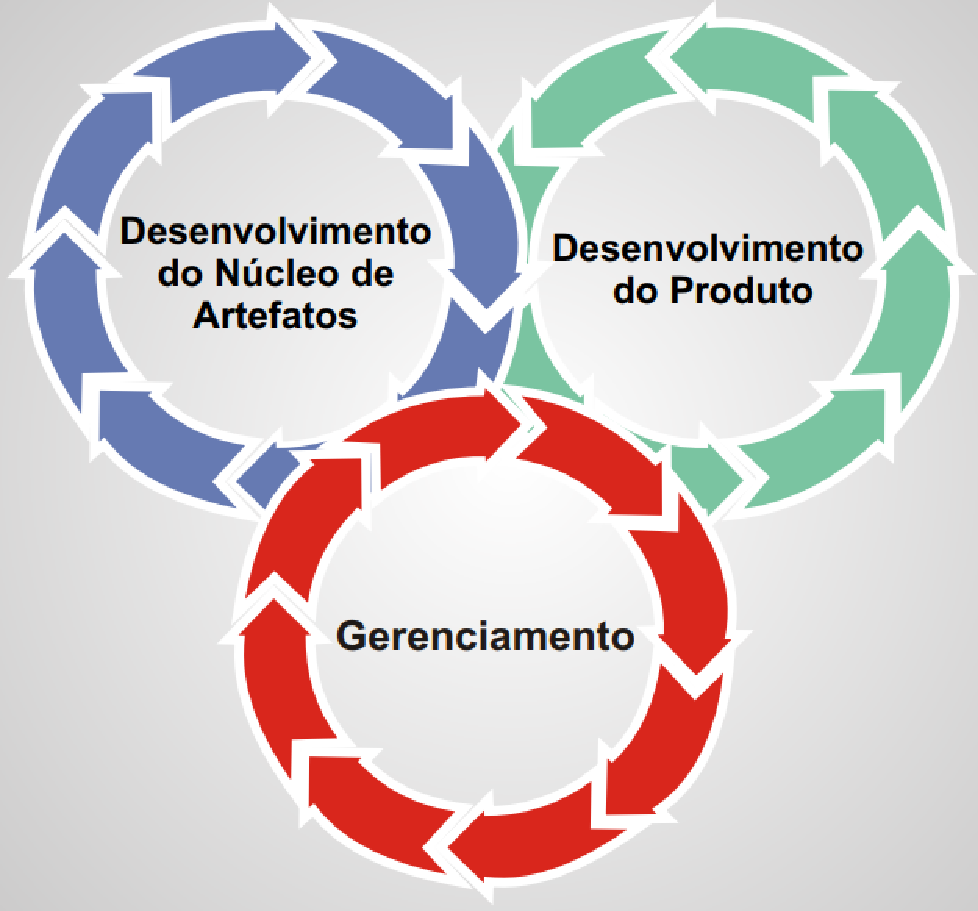
\includegraphics[scale=0.70]{sei.pdf}
	\caption{Adaptado de (SEI 2010) }
	\label{fig:sei}
\end{figure}

\begin{itemize}
	\item \textbf{Engenharia de Domínio} processo em que as similaridades e as variabilidades das LPSs são identificadas e realizadas. No qual, é composto de cinco subprocessos principais, sendo eles: Gerenciamento de Produto, Engenharia de Requisitos do Domínio, Projeto do Domínio, Realização do Domínio e Teste de Domínio;
	\item \textbf{Engenharia de Aplicação} processo em que as aplicações de uma LPS são construídas por meio da reutilização de artefatos de domínio, explorando as variabilidades de uma linha de produto. No qual, é composto pelas subprocessos: Engenharia de Requisitos da Aplicação, Projeto da Aplicação, Realização da Aplicação e Teste da Aplicação.
\end{itemize}

\cite{pohl2005software} desenvolveram um \textit{framework} para engenharia de LPS, cujo objetivo é incorporar os conceitos centrais da engenharia de linha de produto tradicional, proporcionando a reutilização de artefatos e a customização em massa por meio de variabilidades (\ref{fig:lps}).


\begin{figure}[htb]
	\centering
	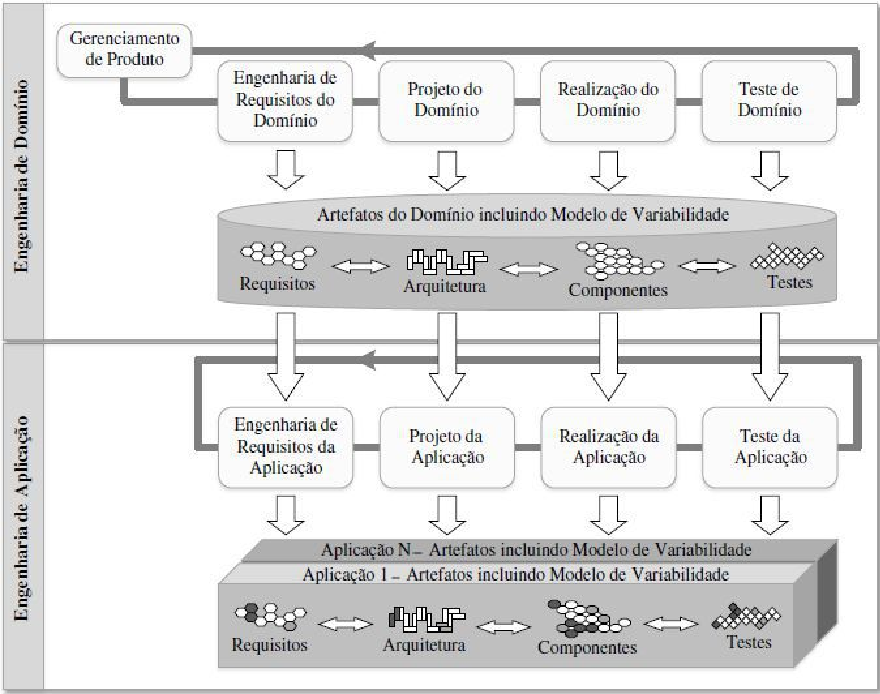
\includegraphics[scale=0.90]{lps.pdf}
	\caption{\textit{Framework} de Engenharia de LPS \cite{pohl2005software}. Traduzido por Geraldi (2015)}
	\label{fig:lps}
\end{figure}

A adoção de LPS traz benefícios em diversos aspectos do processo de desenvolvimento de software, tais como \cite{linden2007product, pohl2005software}:

\begin{itemize}
	\item redução dos custos de desenvolvimento, devido ao reúso de artefatos de um núcleo;
	\item melhoria da qualidade dos produtos, pois os artefatos produzidos são revisados e testados em vários produtos;
	\item redução do tempo de produção (\textit{time to market}) que é mais alto inicialmente, pois os artefatos comuns devem ser construídos antes. Mas, reduz ao produzir cada novo produto;
	\item redução do esforço de manutenção, pois quando um artefato do núcleo for modificado, as mudanças podem ser propagadas para todos os produtos que utilizam tal artefato;
	\item  contribuição para evolução, pois ao inserir um novo produto no núcleo da LPS, concede a oportunidade de evolução de todos os tipos de produtos derivados da LPS
	\item  contribuição para redução da complexidade, devido ao crescente número de solicitações de clientes, a complexidade dos produtos aumenta. Dessa forma, mais funcionalidades são adicionadas ao software. O fato de partes comuns serem 	reusadas por uma LPS ocorre a redução significativa da complexidade;
	\item melhoria na estimativa de custo, pois a organização pode se concentrar em promover produtos que são fáceis de ser gerados a partir da LPS e produtos que exijam extensões podem ser vendidos por preços mais altos; e 
	\item benefícios para os clientes, pois adquirem produtos adaptados às suas necessidades e expectativas por preços acessíveis devido a abordagem de LPS contribuir na redução de custos de desenvolvimento.
\end{itemize}

O núcleo de artefatos é composto de um conjunto de características comuns (similaridades) e características variáveis (variabilidades) \cite{linden2007product}. Esse núcleo forma a base da LPS e inclui a arquitetura de LPS, componentes reusáveis, modelos de domínios, requisitos da LPS, planos de testes e modelos de características e de variabilidades.

De acordo com \cite{apel2016feature}, "uma característica  é um comportamento visível ao usuário final de um sistema de software". Uma característica pode ser obrigatória, opcional ou alternativa. O modelo de características representa as variabilidades de uma LPS. Variabilidades são descritas por: Ponto de variação, o que permite a resolução de variabilidades em artefatos genéricos de uma LPS; Variante, que representa os possíveis elementos que podem ser escolhidos para resolver um ponto de variação e; Restrições entre variantes que estabelecem os relacionamentos entre uma ou mais variantes com o objetivo de resolver seus respectivos pontos de variação ou variabilidade em um dado tempo de resolução \cite{linden2007product,pohl2005software,apel2016feature}.

Analisando o contexto apresentado, podemos considerar que a variabilidade é algo muito importante para não ser levado em consideração quando falamos em qualidade de software. \textcolor{red}{Existem várias abordagens para o gerenciamento de variabilidade***citar quais são***}, uma delas é a \textit{Stereotype-based Management of Variability} (\textit{SMarty}), que realiza o gerenciamento de variabilidades de uma LPS de forma clara e explícita em modelos UML \cite{junior2010systematic}. \textit{SMarty} é composta de um perfil UML, o \textit{SMartyProfile}, e do processo denominado \textit{SMartyProcess}. Ela guia o usuário por meio do \textit{SMartyProcess} na identificação e representação de variabilidades em modelos UML de uma LPS. O perfil \textit{SMartyProfile} é formado por um conjunto de estereótipos e meta-atributos para representar variabilidades em modelos UML de LPS.

Por meio da UML e seu mecanismo de perfil \textit{SMarty} permite a representação explícita de variabilidades. O \textit{SMartyProcess} é um processo sistemático que guia o usuário na identificação, delimitação, representação, rastreamento de variabilidades e análise de configurações de produtos de uma LPS \textcolor{red}{explicar melhor essa figura (\ref{fig:smartyprocess}). e a 2.4 também} Nele há um conjunto de diretrizes que permitem ao usuário a aplicação dos estereótipos do \textit{SMartyProfile} de forma clara e objetiva e é possível perceber todos os estereótipos suportados pelo perfil na região inferior da (\ref{fig:smartyprofile}). Mais informações relacionadas a \textit{SMarty} podem ser encontradas no anexo \ref{Abordagem_SMarty} - Abordagem \textit{SMarty}, assim como um exemplo de modelagem utilizando a abordagem.

\begin{figure}[htb]
	\centering
	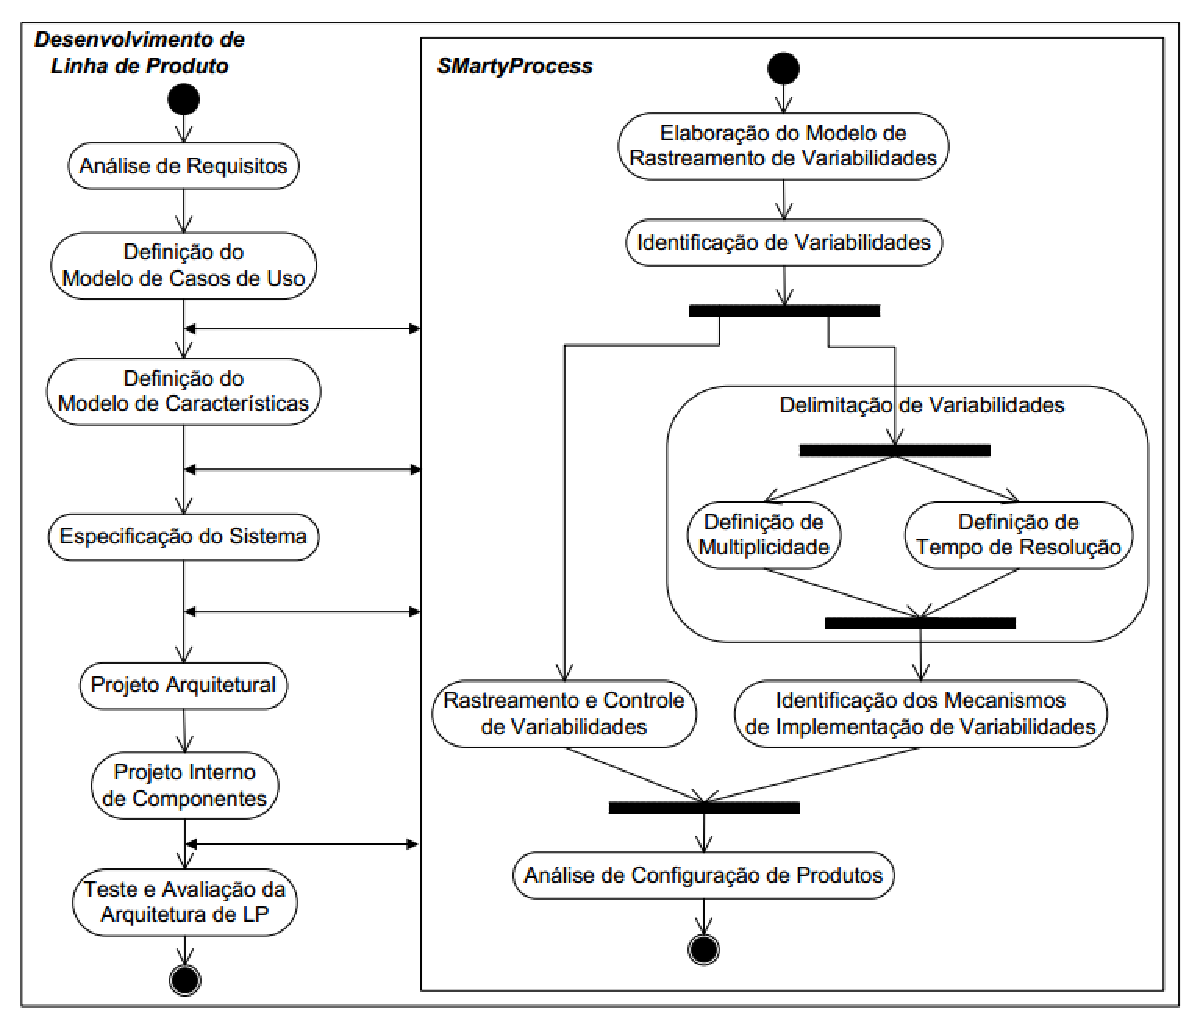
\includegraphics[scale=0.60]{smartyprocess.pdf}
	\caption{ O Processo de Gerenciamento de Variabilidades SMartyProcess e sua Interação entre as Atividades com o Processo de Desenvolvimento de LPS, traduzido de (OliveiraJr et al., 2010b)}
	\label{fig:smartyprocess}
\end{figure}


\begin{landscape}
	
	\begin{figure}[htb]
		\centering
		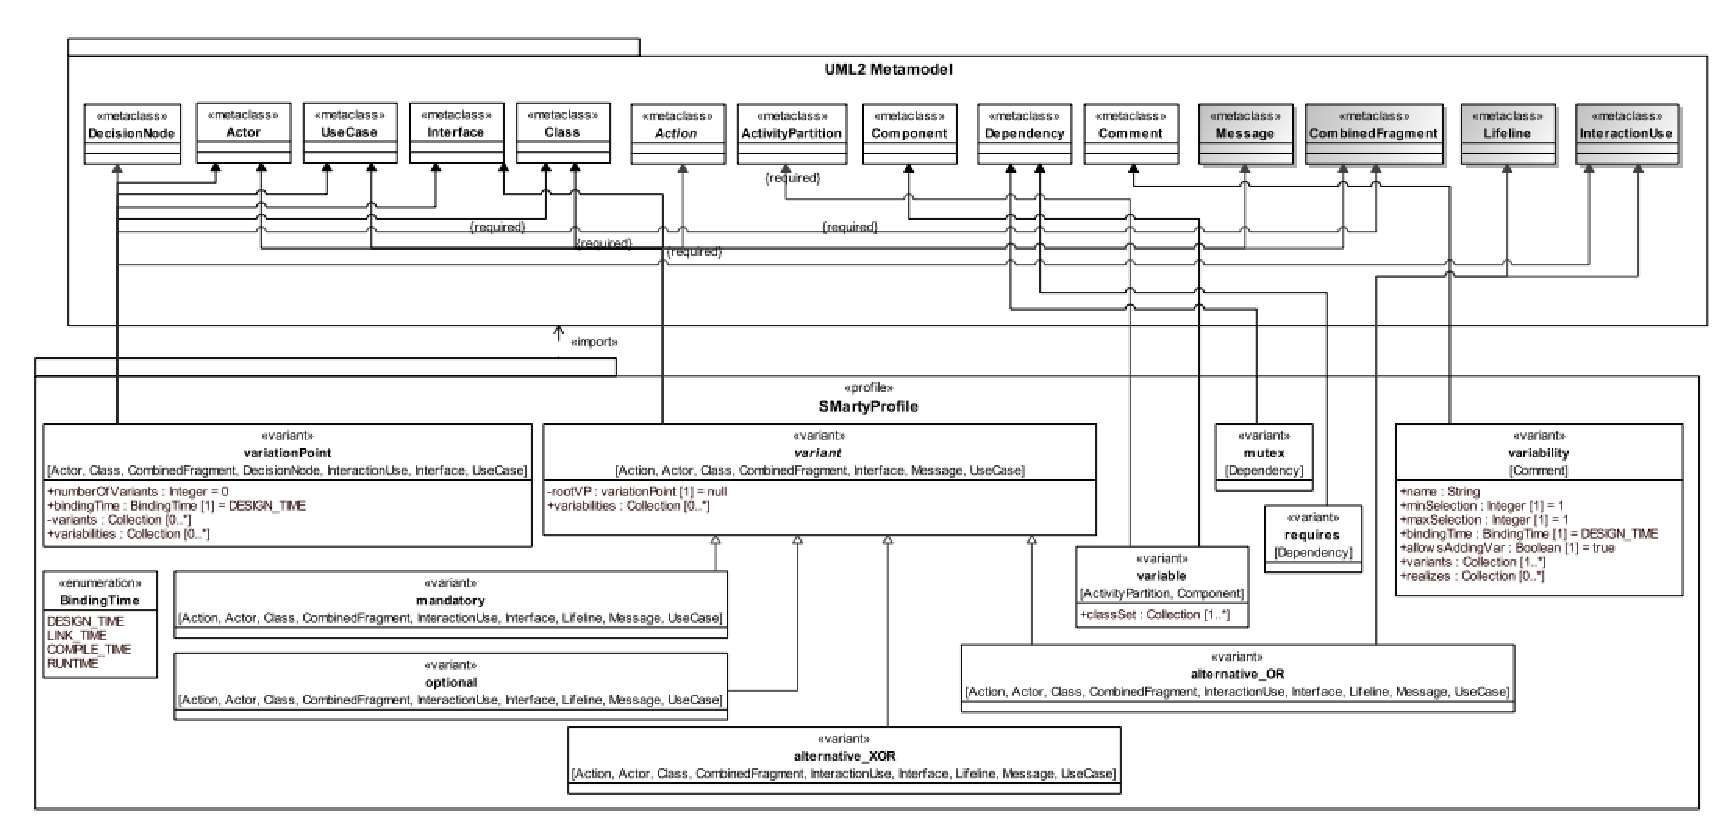
\includegraphics[scale=0.80]{smartyprofile.pdf}
		\caption{ Estereótipos e Meta-Atributos do Perfil SMartyProfile 5.1 com Suporte a Modelos de Casos de Uso, Classes, Componentes, Atividades e Sequência (Fiori et al., 2012; Marcolino, 2014; OliveiraJr et al., 2010a, 2013a). }
		\label{fig:smartyprofile}
	\end{figure}
	
	
\end{landscape}

\section{Teste de Linha de Produto de Software (LPS)}

contextualizar aqui os conceitos de teste

citar os principais itens da revisão sistemática que aborda testes em LPS

tentar contextualizar o teste de linha de produto de software com um exemplo em figura

\section{Teste baseado em Modelos para LPS}

LPS é um interesse da indústria pelo o potencial de reuso de artefatos além de aumentar a produtividade. Para alcançar as melhorias pretendidas, a qualidade dos artefatos reutilizáveis deve ser verificado. Portanto, a garantia de qualidade em geral. Testes em particular, ainda é a técnica de garantia de qualidade mais comum na indústria, são cruciais para os esforços de LPS \cite{delamaro2017introduccao}.

Sendo assim, para uma busca completa do desenvolvimento de teste em LPS primeiro temos que entender mais sobre o modelo de processo de teste. Atualmente existem vários modelos, porém, aqui iremos demonstrar um exemplo utilizando o modelo em V \ref{fig:testeV}.

\begin{figure}[htb]
	\centering
	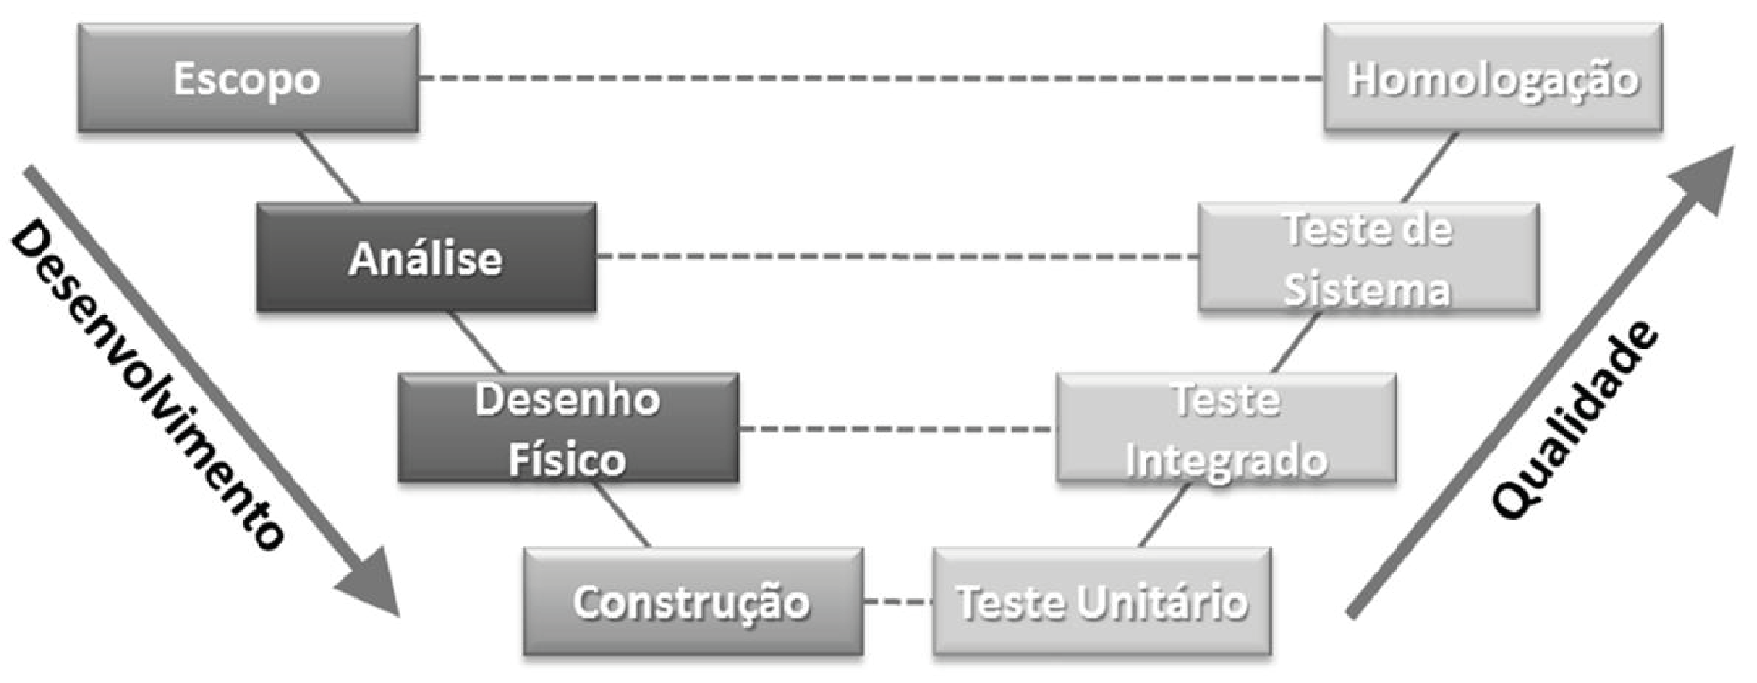
\includegraphics[scale=0.75]{teste.pdf}
	\caption{ Esquema simplificado que representa o modelo V }
	\label{fig:testeV}
\end{figure}

O modelo V é um modelo conceitual de Engenharia de sistemas/desenvolvimento de produto visto como melhoria ao problema de reatividade do modelo em cascata. Ele permite que, durante a integração de um sistema em seus diversos níveis, os testes sejam feitos contra os próprios requisitos do componente/interface que está sendo testado(a), em contraste com modelos anteriores onde o componente era testado contra a especificação do componente/interface.

Para este trabalho, a intenção é a antecipação dos testes como no modelo V \ref{fig:testeV} utilizando o modelo de teste consideramos duas etapas, a verificação e a validação. Aqui iremos tratar a validação, e por se tratar de teste de funcionalidade em engenharia de domínio, iremos utilizar a técnica de caixa preta,  onde em um processo de teste \ref{fig:testelps} na preparação do teste sabe-se apenas os parâmetros de entrada não temos acesso a parte interna do processo de execução, apenas o resultado esperado em sua saída para registro posterior do teste.


\begin{figure}[htb]
	\centering
	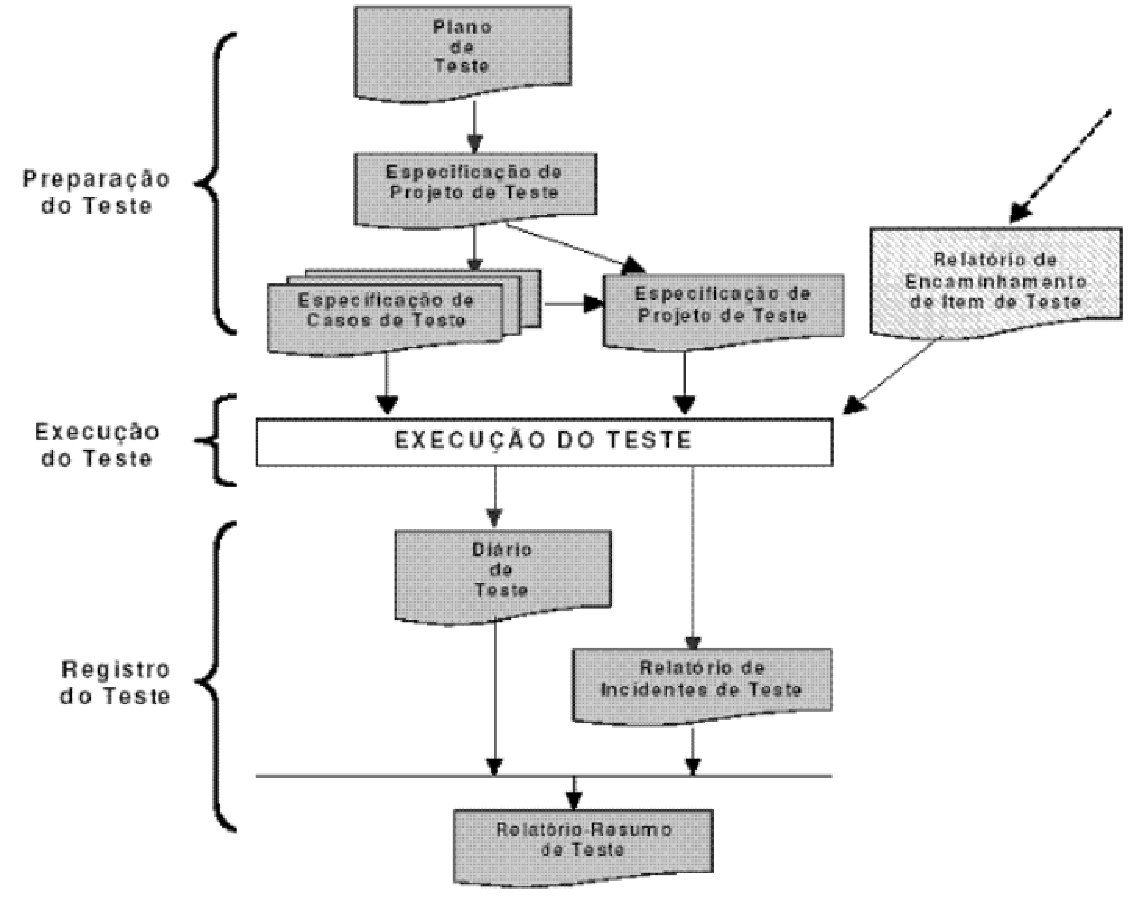
\includegraphics[scale=0.55]{testelps.pdf}
	\caption{ Modelo de proposta de implantação do processo de teste de software segundo \cite{crespo2004metodologia}}
	\label{fig:testelps}
\end{figure}

Sabendo-se que será utilizando teste caixa-preta, o nível de teste trabalhado poderá ser o de sistema, embora iremos trabalhar com diagramas mais detalhados como o de sequência. Pensando neste sentido de trabalho de teste a nível de engenharia de Domínio, procuramos buscar alternativas de teste que não necessitassem de atuação a nível de código ou caixa-branca.

\citealp{do2014strategies} cita em um trabalho de revisão de literatura relacionando teste em LPS, buscam analisar as estratégias de testes que são abordadas e quais seus potenciais em uma maior taxa de detecção de erros. Nesse casso eles apontam que testes devem ser considerados tanto na engenharia de domínio como na de aplicação. Dentro do interesse de teste dois itens devem ser levados em consideração, o conjunto de requisitos do produto e a qualidade do modelo de variabilidade em teste, isso demonstra que teste a nível de modelagem é uma item a ser pesquisado.

\citealp{do2014strategies} apresentam também um grande número de técnicas para lidar com o aspecto de seleção de produto para teste e o teste real dos produtos. No entanto, faltam relatos reais de experiências industriais que limitam algumas conclusões. O estudo ainda apresenta uma série de estratégias que podem apoiar a seleção e a execução dos testes reais em produtos.

O Teste Baseado em Modelo (TBM) é uma forma de teste de software em que os casos de teste são derivados de um modelo que descreve aspectos (geralmente funcionais) do sistema sendo testado. Tais casos são conhecidos como a suíte abstrata de testes, e seu nível de abstração está intimamente relacionado ao nível de abstração do modelo, segundo \citealp{do2014strategies}. As vantagens da abordagem é que a geração de testes começa mais cedo no ciclo do desenvolvimento e pode-se criar casos de teste automaticamente a partir do modelo, isso vai de encontro com nosso interesse, que é a antecipação da etapa de teste. 

Os casos de teste podem ser representados por meio de árvores de decisão, \textit{statecharts}, ontologias de domínio ou diagramas de casos de uso e/ou estados da UML (\textit{Unified Modeling Language})\cite{isa2017model}.

Baseado neste cenário, um dos maiores desafios em teste de LPS se dá em relação as particularidades de cada modelo, para isso TBM busca na criação de modelos dentro da engenharia de domínio, realizar a geração de casos de teste que possam ser reutilizados na engenharia de aplicação, foco da nossa pesquisa. Alguns trabalhos realizados focam na construção da geração antecipada dos teste na modelagem de domínio da LPS, onde, o foco das pesquisas ficam em relação a como conseguir gerar reutilização com uma maior cobertura dos possíveis problemas.

Uma particularidade de TBM é que ele se faz de uso de Máquinas de Estado Finito (MEF) \ref{fig:tbmmef}, um modelo formal que representa as possíveis configurações do sistema.

\begin{figure}[htb]
	\centering
	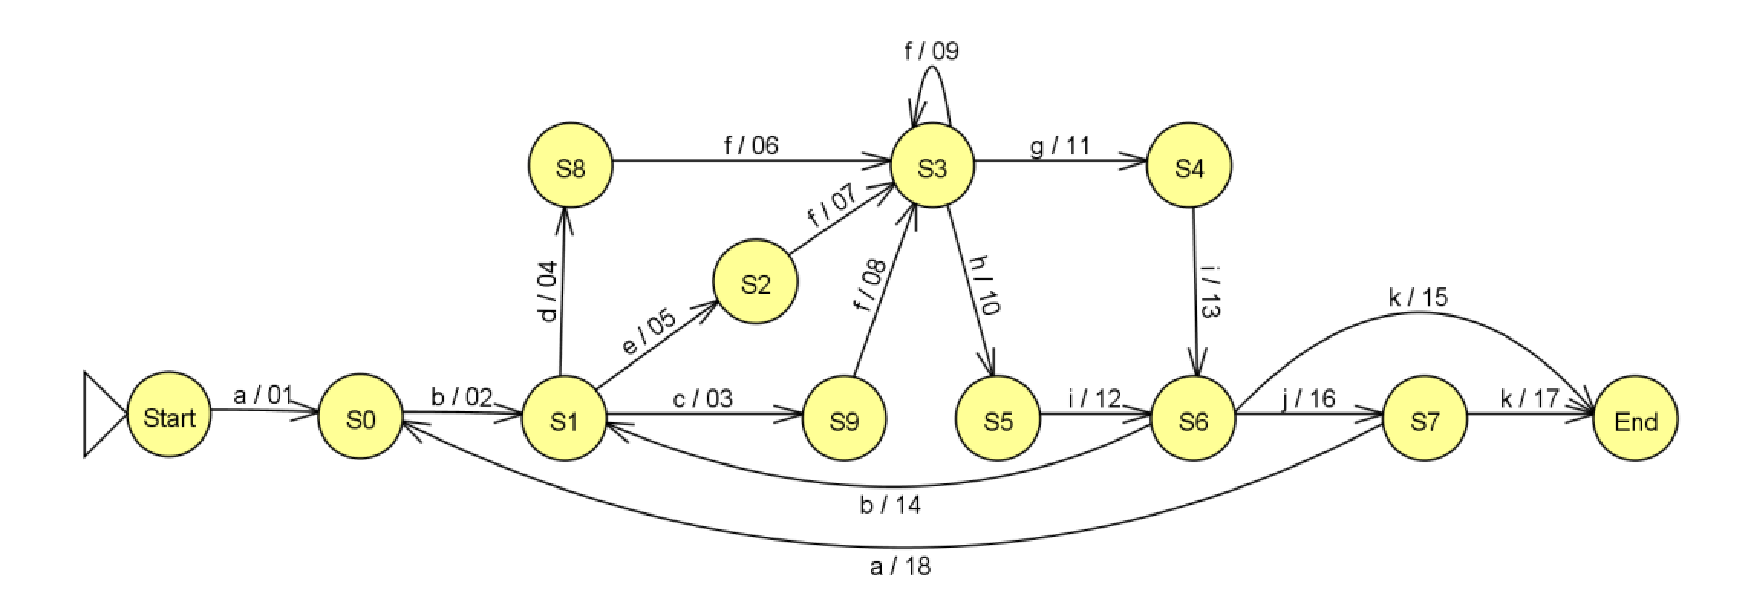
\includegraphics[scale=0.50]{fsm.pdf}
	\caption{ Exemplo de uma MEF utilizado por \citealp{costa2016split}}
	\label{fig:tbmmef}
\end{figure}

Sabendo que TBM possui características na utilização em LPS e que proporciona uma certa relação com variabilidade, preenchendo os principais requisitos para nossa pesquisa, foi conduzido um MSL Seção \ref{sec:MSL}, com a finalidade de evidenciar como que TBM esta sendo utilizado em LPS. Onde, ao longo de toda o MSL foram encontrados vários estudos que indicam a utilizam de TBM para LPS com tratativa da variabilidade.

Os estudos \textcolor{red}{quais estudos reportam do MSL} reportam que, em grande maioria, a partir de um modelo é realizado a conversão para um artefato, normalmente máquina de estado finito estendido, assim, ele pode ser verificado os pontos de variação e variabilidade. Após, gerenciado essa variabilidade com ou sem a utilização de uma ferramenta de apoio. E por fim, a criação do caso de teste, fazendo o uso ou não de rastreabilidade.

Para facilitar a leitura, os estudos utilizados para a extração de dados estão contidos na \ref{table:listaextraquali} que é um conjunto de estudos restante de todo o processo de mapeamento, e que reportam o TBM em LPS, assim foi criado um guia visual na \ref{fig:guiaestudo} onde apresenta um mapa com o que os trabalhos do MSL reportaram, contido na Anexo \ref{sec:roadmap} \textcolor{red}{*** reescrever ***}Porém, caso o leitor queira mais detalhes sobre o guia ou os trabalhos, ele pode consultar o MSL no Anexo \ref{sec:MSL}

A \ref{fig:guiaestudo} Apresenta um compilado de todos os trabalhos resultantes da MS organizados por tópicos chaves, considerando o interesse do leitor, um exemplo, caso o leitor queira saber quais trabalhos que utilizam de gerenciamento de variabilidade ele terá um item no gráfico apontando para este item.


\begin{landscape}
	\scalefont{0.7}
	\begin{longtable}[c]{|c|l|l|c|c|c|}
		\caption{Trabalhos selecionados para leitura e extração de dados}
		\label{table:listaextraquali}\\
		\hline
		\textbf{ID} & \multicolumn{1}{c|}{\textbf{Título}} & \multicolumn{1}{c|}{\textbf{Autor(res)}} & \textbf{\begin{tabular}[c]{@{}c@{}}Ano de \\ Publicação\end{tabular}} & \textbf{Fonte} & \textbf{Tipo} \\ \hline
		\endfirsthead
		%
		\hline
		\textbf{ID} & \multicolumn{1}{c|}{\textbf{Título}} & \multicolumn{1}{c|}{\textbf{Autor(res)}} & \textbf{\begin{tabular}[c]{@{}c@{}}Ano de \\ Publicação\end{tabular}} & \textbf{Fonte} & \textbf{Tipo} \\ \hline
		
		\endhead
		%
		T1 & \begin{tabular}[c]{@{}l@{}}Delta-Oriented Model-Based \\ SPL Regression Testing\end{tabular} & \begin{tabular}[c]{@{}l@{}}Sascha Lity, Malte Lochau, \\ Ina Schaefer, Ursula Goltz\end{tabular} & 2012 & ACM & Evento \\ \hline
		T2 & \begin{tabular}[c]{@{}l@{}}Industrial Evaluation of Pairwise \\ SPL Testing with MoSo-PoLiTe\end{tabular} & \begin{tabular}[c]{@{}l@{}}Michaela Steffens, Sebastian Oster, \\ Malte Lochau, Thomas Fogdal\end{tabular} & 2012 & ACM & Evento \\ \hline
		T3 & \begin{tabular}[c]{@{}l@{}}Model-Based Coverage-Driven Test Suíte \\ Generation for Software Product Lines\end{tabular} & \begin{tabular}[c]{@{}l@{}}Harald Cichos, Sebastian Oster, \\ Malte Lochau, Andy Schurr\end{tabular} & 2011 & ACM & Periódico \\ \hline
		T4 & \begin{tabular}[c]{@{}l@{}}MoSo-PoLiTe - Tool Support for \\ Pairwise and Model-Based Software \\ Product Line Testing\end{tabular} & \begin{tabular}[c]{@{}l@{}}Sebastian Oster, Ivan Zorcic, \\ Florian Markert, Malte Lochau\end{tabular} & 2011 & ACM & Evento \\ \hline
		T5 & MPLM - MaTeLo Product Line Manager & Hamza Samih, Ralf Bogusch & 2014 & ACM & Evento \\ \hline
		T6 & \begin{tabular}[c]{@{}l@{}}On the use of test cases in model-based \\ software product line development\end{tabular} & \begin{tabular}[c]{@{}l@{}}Alexander Knapp, Markus Roggenbach, \\ Bernd-Holger Schlingloff\end{tabular} & 2014 & ACM & Evento \\ \hline
		T7 & \begin{tabular}[c]{@{}l@{}}Pairwise Feature-Interaction Testing \\ for SPLs: Potentials and Limitations\end{tabular} & \begin{tabular}[c]{@{}l@{}}Sebastian Oster, Malte Lochau, \\ Marius Zink, Mark Grechanik\end{tabular} & 2011 & ACM & Evento \\ \hline
		T8 & \begin{tabular}[c]{@{}l@{}}Deriving Usage Model Variants for \\ Model- based Testing: An Industrial Case Study\end{tabular} & \begin{tabular}[c]{@{}l@{}}Hamza Samih,  Hélène Le Guen, \\ Ralf Bogusch, Mathieu Acher, Benoit Baudry\end{tabular} & 2014 & IEEE & Evento \\ \hline
		T9 & \begin{tabular}[c]{@{}l@{}}Model-based Software Product Line \\ Testing by Coupling Feature Models \\ with Hierarchical Markov Chain Usage Models\end{tabular} & Ceren Sahin Gebizli, Hasan Sozer & 2016 & IEEE & Evento \\ \hline
		T10 & \begin{tabular}[c]{@{}l@{}}Model-Based Test Design of Product Lines: \\ Raising Test Design to the Product Line Level\end{tabular} & \begin{tabular}[c]{@{}l@{}}Hartmut Lackner, Martin Thomas, \\ Florian Wartenberg, Stephan Weißleder\end{tabular} & 2014 & IEEE & Periódico \\ \hline
		T11 & Requirements-Based Delta-Oriented SPL Testing & \begin{tabular}[c]{@{}l@{}}Michael Dukaczewski, Ina Schaefer, \\ Remo Lachmann, Malte Lochau\end{tabular} & 2013 & IEEE & Evento \\ \hline
		T12 & \begin{tabular}[c]{@{}l@{}}Using Feature Model to Support Model- Based \\ Testing of Product Lines: An Industrial Case Study\end{tabular} & \begin{tabular}[c]{@{}l@{}}Shuai Wang,  Shaukat Ali,\\  Tao Yue, Marius Liaaen\end{tabular} & 2013 & IEEE & Periódico \\ \hline
		T13 & \begin{tabular}[c]{@{}l@{}}An automated Model-based Testing \\ Approach in Software Product Lines \\ Using a Variability Language\end{tabular} & \begin{tabular}[c]{@{}l@{}}Boni García,  Rodrigo García-Carmona, \\ Álvaro Navas, Hugo A. Parada-Gélvez,\\  Félix Cuadrado, Juan C. Dueñas\end{tabular} & 2010 & \begin{tabular}[c]{@{}c@{}}Politécnica \\ Arquivo \\ digital UPM\end{tabular} & Evento \\ \hline
		T14 & \begin{tabular}[c]{@{}l@{}}Automated Product Line Methodologies \\ to Support Model-Based Testing\end{tabular} & Shuai Wang,  Shaukat Ali, Arnaud Gotlieb & 2013 & \begin{tabular}[c]{@{}c@{}}CEUR \\ Event Proceedings\end{tabular} & Evento \\ \hline
		T15 & \begin{tabular}[c]{@{}l@{}}Behavioural Model Based \\ Testing of Software Product Lines\end{tabular} & Xavier Devroey & 2014 & ACM & Evento \\ \hline
		T16 & \begin{tabular}[c]{@{}l@{}}Feature Model-based \\ Software Product Line Testing\end{tabular} & SEBASTIAN OSTER & 2012 & TUprints & Periódico \\ \hline
		T17 & \begin{tabular}[c]{@{}l@{}}Model-based pairwise testing for feature interaction \\ coverage in software product line engineering\end{tabular} & \begin{tabular}[c]{@{}l@{}}Malte Lochau, Sebastian Oster, \\ Ursula Goltz, Andy Schurr\end{tabular} & 2011 & Springer & Periódico \\ \hline
		T18 & Model-based Test Generation for Software Product Line & Xinying Cai, Hongwei Zeng & 2013 & IEEE & Evento \\ \hline
		T19 & Model-Based Testing for Software Product Lines & Erika Mir Olimpiew & 2008 & Springer & Evento \\ \hline
		T20 & PLETS - A Product line of model-based testing tools & Elder de Macedo Rodrigues & 2013 & PUC-RS & Evento \\ \hline
		T21 & \begin{tabular}[c]{@{}l@{}}Top-Down and Bottom-Up Approach for \\ Model-Based Testing of Product Lines\end{tabular} & Stephan Weißleder, Hartmut Lackner & 2013 & EPTCS & Evento \\ \hline
		T22 & \begin{tabular}[c]{@{}l@{}}A Product Line Modeling and Configuration  Methodology \\ to Support Model-Based  Testing: An Industrial Case Study\end{tabular} & \begin{tabular}[c]{@{}l@{}}Shaukat Ali, Tao Yue, Lionel Briand, \\ Suneth Walawege\end{tabular} & 2012 & Springer & Periódico \\ \hline
		T23 & \begin{tabular}[c]{@{}l@{}}Coverage Criteria for Behavioural \\ Testing of Software Product Lines\end{tabular} & \begin{tabular}[c]{@{}l@{}}Xavier Devroey, Gilles Perrouin, \\ Axel Legay, Maxime Cordy, \\ Pierre-Yves Schobbens, Patrick Heymans\end{tabular} & 2014 & Springer & Evento \\ \hline
		T24 & \begin{tabular}[c]{@{}l@{}}A Model Based Testing Approach for Model-Driven \\ Development and Software Product Lines\end{tabular} & \begin{tabular}[c]{@{}l@{}}Beatriz Pérez Lamancha,  Macario Polo Usaola, \\ Mario Piattini Velthius\end{tabular} & 2010 & Springer & Evento \\ \hline
		T25 & \begin{tabular}[c]{@{}l@{}}A Vision for Behavioural Model-Driven \\ Validation of Software Product Lines\end{tabular} & \begin{tabular}[c]{@{}l@{}}Xavier Devroey, Maxime Cordy,  \\ Gilles Perrouin, Eun-Young Kang, \\ Pierre-Yves Schobbens, Patrick Heymans, \\ Axel Legay,  Benoit Baudry\end{tabular} & 2012 & Springer & Evento \\ \hline
		T26 & \begin{tabular}[c]{@{}l@{}}Abstract Test Case Generation for Behavioural \\ Testing of Software Product Lines\end{tabular} & \begin{tabular}[c]{@{}l@{}}Xavier Devroey, Gilles Perrouin, \\ Pierre-Yves Schobbens\end{tabular} & 2014 & ACM & Evento \\ \hline
		T27 & \begin{tabular}[c]{@{}l@{}}Applying Incremental Model Slicing to \\ Product-Line Regression Testing\end{tabular} & \begin{tabular}[c]{@{}l@{}}Sascha Lity, Thomas Morbach,  \\ Thomas Th¨ um, Ina Schaefer\end{tabular} & 2016 & Springer & Periódico \\ \hline
		T28 & \begin{tabular}[c]{@{}l@{}}Automated Testing of Software-as- a-Service \\ Configurations using a Variability Language\end{tabular} & Sachin Patel, Vipul Shah & 2015 & ACM & Evento \\ \hline
		T29 & Delta-Oriented FSM-Based Testing & \begin{tabular}[c]{@{}l@{}}Mahsa Varshosaz,  Harsh Beohar, \\ Mohammad Reza Mousavi\end{tabular} & 2015 & Springer & Evento \\ \hline
		T30 & \begin{tabular}[c]{@{}l@{}}Incremental Model-Based Testing of \\ Delta-oriented Software Product Lines\end{tabular} & \begin{tabular}[c]{@{}l@{}}Malte Lochau, Ina Schaefer, \\ Jochen Kamischke, Sascha Lity\end{tabular} & 2012 & Springer & Periódico \\ \hline
		T31 & Model Based Testing in Software Product Lines & \begin{tabular}[c]{@{}l@{}}Pedro Reales, Macario Polo, \\ Danilo Caivano\end{tabular} & 2011 & Springer & Evento \\ \hline
		T32 & Model-Based Testing & \begin{tabular}[c]{@{}l@{}}Malte Lochau, Sven Peldszus, \\ Matthias Kowal,  Ina Schaefer\end{tabular} & 2014 & Springer & Evento \\ \hline
		T33 & \begin{tabular}[c]{@{}l@{}}Parameterized Preorder Relations for \\ Model-Based Testing of Software Product Lines\end{tabular} & Malte Lochau, Jochen Kamischke & 2012 & Springer & Evento \\ \hline
		T34 & Poster: VIBeS, Transition System Mutation Made Easy & \begin{tabular}[c]{@{}l@{}}Xavier Devroey, Gilles Perrouin, \\ Pierre-Yves Schobbens, Patrick Heymans\end{tabular} & 2015 & IEEE & Evento \\ \hline
		T35 & Spinal Test Suites for Software Product Lines & Harsh Beohar, Mohammad Reza Mousavi & 2014 & EPTCS & Evento \\ \hline
		T36 & \begin{tabular}[c]{@{}l@{}}Automated model-based testing\\ using the  UML testing profile and QVT\end{tabular} & \begin{tabular}[c]{@{}l@{}}Beatriz Pérez Lamancha, Pedro Reales Mateo, \\ IgnacioRodríguez de Guzmán, Macario Polo Usaola, \\ Mario Piattini Velthius\end{tabular} & 2009 & ACM & Evento \\ \hline
		T37 & \begin{tabular}[c]{@{}l@{}}Relating Variability Modeling and \\ Model- Based Testing for Software Product Lines Testing\end{tabular} & Hamza Samih & 2012 & ICTSS & Evento \\ \hline
		T38 & \begin{tabular}[c]{@{}l@{}}An Evaluation of Model-Based \\ Testing in Embedded Applications\end{tabular} & Stephan Weißleder, Holger Schlingloff & 2014 & IEEE & Evento \\ \hline
		T39 & \begin{tabular}[c]{@{}l@{}}Assessing Software Product Line Testing Via Model-Based \\ Mutation An Application to Similarity Testing\end{tabular} & \begin{tabular}[c]{@{}l@{}}Christopher Henard, Mike Papadakis, \\ Gilles Perrouin, Jacques Klein, Yves Le Traon\end{tabular} & 2013 & IEEE & Evento \\ \hline
		T40 & \begin{tabular}[c]{@{}l@{}}Automated and Scalable T-wise Test Case Generation \\ Strategies for Software Product Lines\end{tabular} & \begin{tabular}[c]{@{}l@{}}Gilles Perrouin, Sagar Sen, Jacques Klein, \\ Benoit Baudry, Yves le Traon Lassy\end{tabular} & 2010 & IEEE & Evento \\ \hline
		T41 & \begin{tabular}[c]{@{}l@{}}Model-based Testing of System Requirements \\ using UML Use Case Models\end{tabular} & Bill Hasling, Helmut Goetz, Klaus Beetz & 2008 & IEEE & Evento \\ \hline
		T42 & \begin{tabular}[c]{@{}l@{}}Successive refinement of models for model-based \\ testing to increase system test effectiveness\end{tabular} & \begin{tabular}[c]{@{}l@{}}Ceren Sahin Gebizli, Hasan Sozer, \\ Ali Ozer Ercan\end{tabular} & 2016 & IEEE & Evento \\ \hline
		T43 & A Software Product Line for Model-Based Testing Tools & \begin{tabular}[c]{@{}l@{}}Elder M. Rodrigues, Avelino F. Zorzo, \\ Itana M. Gimenez, Elisa Y. Nakagawa, \\ Flavio M. Oliveira, José C. Maldonado\end{tabular} & 2012 & PUC-RS & Outro \\ \hline
		T44 & \begin{tabular}[c]{@{}l@{}}Reusing State Machines for Automatic \\ Test Generation in Product Lines\end{tabular} & \begin{tabular}[c]{@{}l@{}}Stephan Weißleder, Dehla Sokenou, \\ Bernd-Holger Schlingloff\end{tabular} & 2008 & MoTip & Evento \\ \hline
	\end{longtable}
\end{landscape}

%\begin{landscape}
	
%	\begin{figure}[htb]
%		\centering
%		\caption{Atualizar imagem Guia de estágios do processo de TBM em LPS}
%		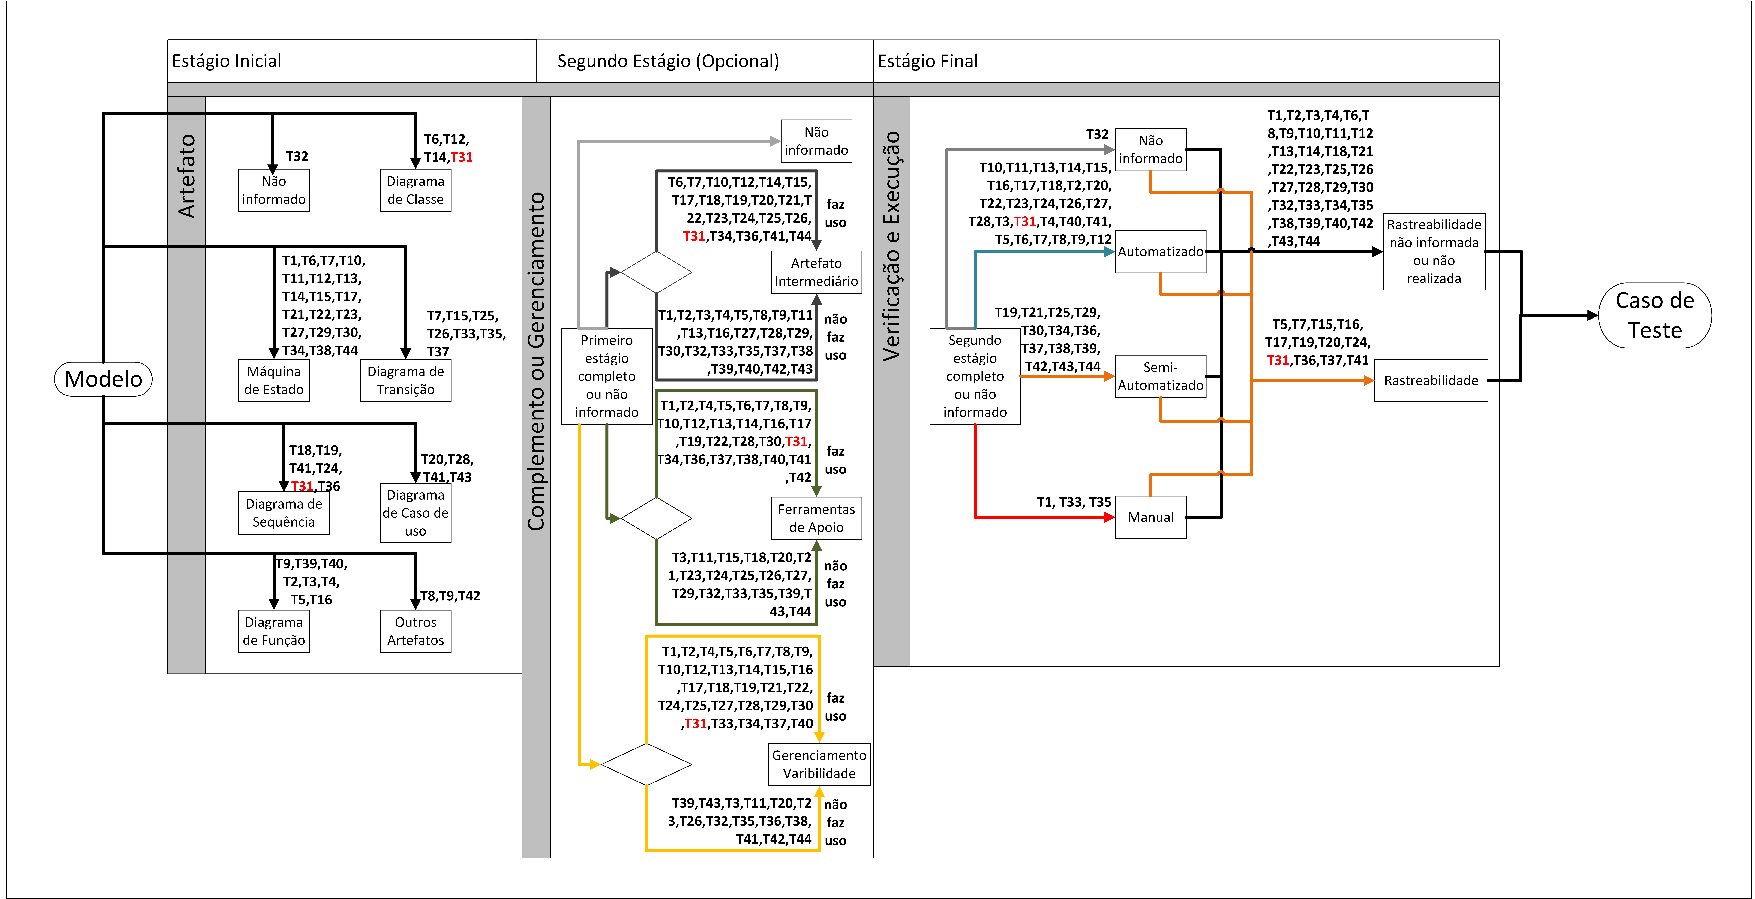
\includegraphics[scale=0.40]{guiaestudo.png}
%		\label{fig:guiaestudoquali}
%	\end{figure}
%	
%\end{landscape}

\section{A Abordagem SPLit-MbT}

\cite{costa2016split} apresenta uma abordagem denominada \textit{Software Product Line Testing Method Based on System Models} (SPLiT-MBt) onde é possível gerar casos de teste funcional e \textit{scripts} para testar os produtos derivados de uma LPS, onde os casos de teste comuns entre os produtos derivados são gerados com base no reuso inerente a LPS.

\begin{figure}[htb]
	\centering
	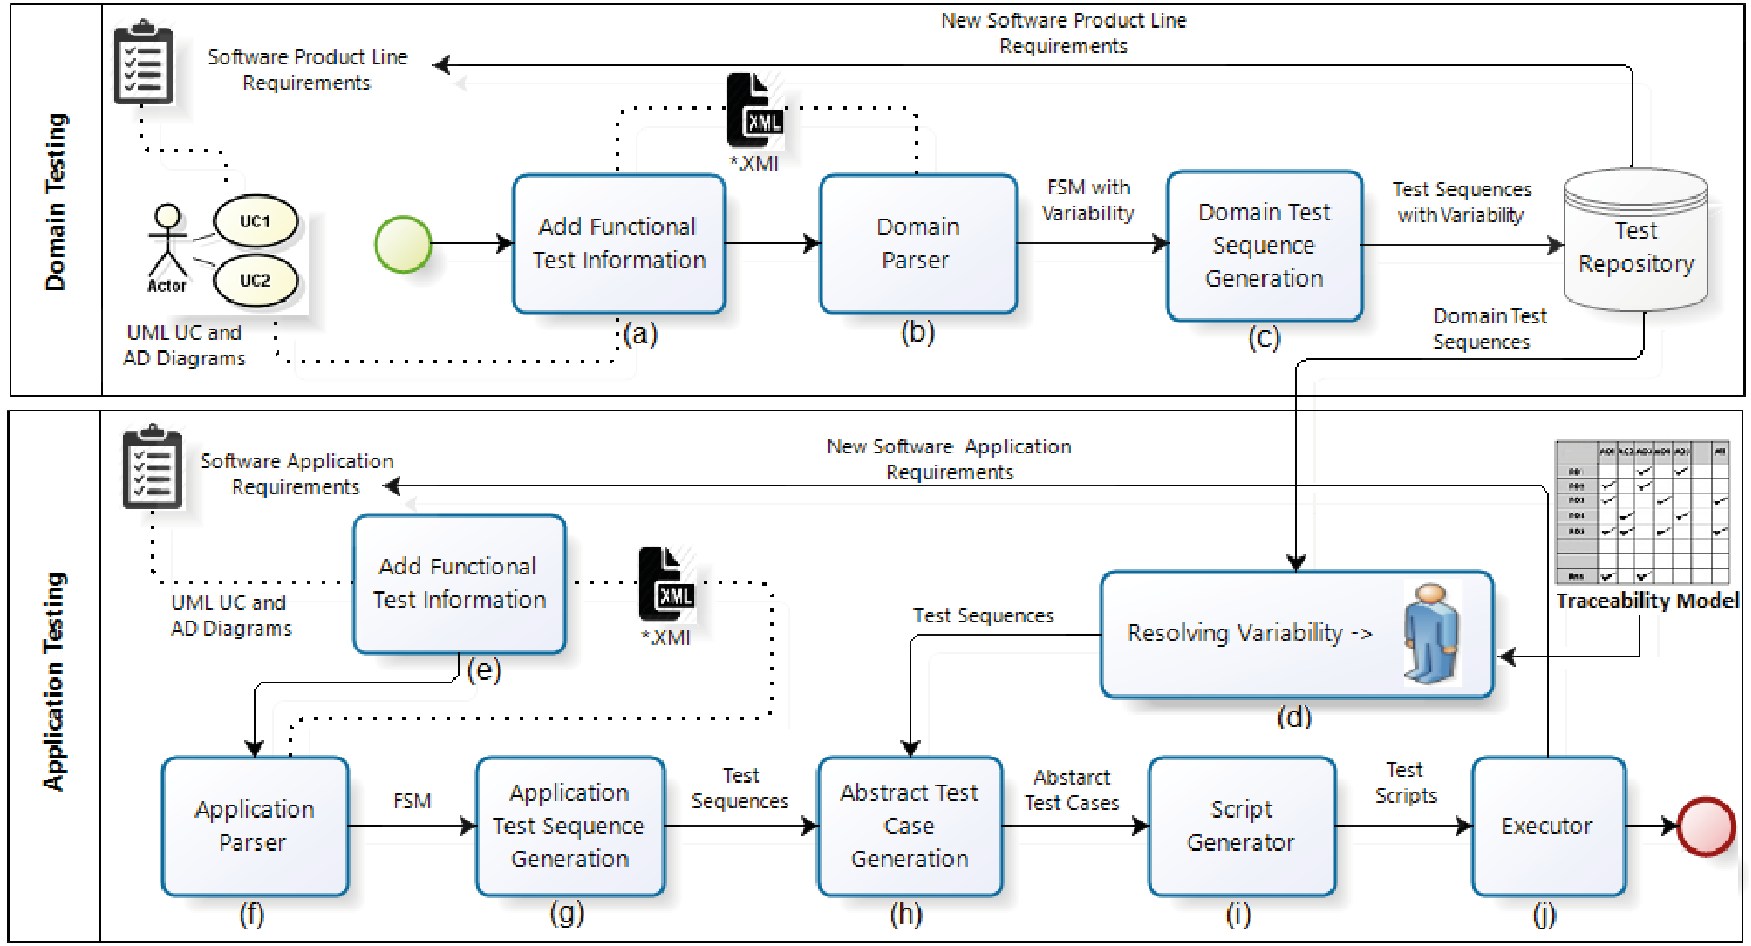
\includegraphics[scale=0.60]{splitmbt.pdf}
	\caption{Panorama da abordagem SPLiT-MBt por \citealp{costa2016split}}
	\label{fig:splitmbt}
\end{figure}

O objetivo principal da abordagem é prover o reuso de artefatos de teste baseado na adaptação do uso de teste baseado em modelo (TBM) para geração automática de casos de teste funcional e \textit{scripts} para modelos considerando a variabilidade.

Para fornecer o reuso ele é aplicado em duas etapas vide \ref{fig:splitmbt}, onde na primeira é realizada a anotação em modelo de sistema, as informações de variabilidade e teste, em seguida utilizadas para gerar sequências de teste usando diferentes métodos formais, como o HSI, UIO,DS ou TT. O modelo formal utilizado é Máquina de Estado Finito e que são estendidas para lidar com as informações sobre variabilidade, uma vez que os modelos de entrada esperado é que já esteja modelado com base na abordagem \textit{SMarty}.

Na engenharia de domínio um diagrama de atividade é convertido em uma Máquina de estado Finitos (MEF) onde é estendida para lidar com informações sobre variabilidade, em seguida se faz a utilização de um modelo formal de geração de sequência de teste denominado HSI. Então essas sequências de teste são armazenadas em um repositório para reutilização, porém, ainda sem a resolução da variabilidade.

Já na segunda etapa, na engenharia de aplicação, os casos de teste são reaproveitados e assim é gerado uma solução para a variabilidade, os modelos de teste e as sequências geradas são utilizadas para gerar os \textit{scripts} de teste que podem ser executados por diferentes ferramentas de teste funcional. Outro fator que deve ser levado em consideração é a rastreabilidade dos casos de teste, que proporciona uma verificação posterior de quais casos de teste foram reaproveitados e se sofreram atualizações. as diferenças entre este trabalho para com o SPLiT-MBt é que \textit{SMartyTesting} dará suporte ao diagrama de sequência que também é suportado por \textit{SMarty}, a escolha por este tipo de modelo é por proporcionar um maior teor de detalhes relacionado aos processos.

\section{Considerações Finais}
Nesta seção não foi abordado alguns temas como tipos, técnicas ou níveis de teste, pois entendemos que o leitor que venha buscar por este assunto já está familiarizado com os princípios básicos de teste de software.


% Tópico 3




%\chapter{O problema}
\label{sec:PHE}


Este tópico define o problema ...

O tópico está dividido como segue: A seção \ref{sec:PHEpolinomial} apresenta ... 

\section{O problema polinomial}
\label{sec:PHEpolinomial}

Considere os conjuntos $\conj{P}{1}{p}{np}$

\begin{align}
	\textbf{Encontrar} \quad & x_{ptdh} \quad (\interval{1}{p}{np}, ~\interval{1}{t}{nt}, ~\interval{1}{d}{nd}, 				~\interval{1}{h}{nh}) \nonumber \\
	\label{eq:H1_poli}
	\textbf{Sujeito a} \quad & \sum _{d=1}^{nd} \sum _{h=1}^{nh}x_{ptdh}=r_{pt} \quad (\interval{1}{p}{np}, 					~\interval{1}{t}{nt}) \\
	& x_{ptdh} \in \{0,1\} \quad (\interval{1}{p}{np}, ~\interval{1}{t}{nt}, ~\interval{1}{d}{nd}, ~\interval{1}{h}{nh})
\end{align}


\section{O problema de otimização abordado}
\label{sec:PHEreal}

O problema abordado neste trabalho é...

As restrições fortes são definidas a seguir.

\begin{defi}[Restrições fortes]
\label{def:rest_fortes}
São aquelas que devem ser satisfeitas para que...

\end{defi}

% Tópico 4
\chapter{A Abordagem SMartyTesting}
\label{cap3:abordagemsmartytesting}
\pagestyle{plain}

\section{Considerações Iniciais}

Neste tópico é apresentada uma abordagem que auxilia na geração de sequências de teste na Engenharia de Domínio de LPS a partir de modelos \textit{SMarty}. Tais sequências de teste podem ser utilizadas para a geração de casos de teste que, em um segundo momento, podem ser usados na Engenharia de Aplicação. Denominada \textit{SMartyTesting}, a abordagem auxilia na geração de sequências de teste a partir de diagramas de sequência modelados com base em casos de uso e seus fluxos básicos e alternativos, em que o diagrama é convertido para um segundo artefato, diagrama de atividades, que é o requisito de entrada da abordagem SPLiT-MBt. Assim, é realizada a geração de sequências de teste contendo variabilidade. Dessa forma, as sequências de teste podem ser reutilizadas para cada produto a ser testado, aproveitando os benefícios de SPLiT-MBt.

\section{Caracterização da Abordagem \textit{SMartyTesting}}
\label{cap3sec:caracterizacao_smarty}

Nesta seção são abordados os elementos que caracterizam a abordagem \textit{SMartyTesting} como modelos, processos e ferramentas.

\subsection{Definição do Processo Adotado pela Abordagem \textit{SMartyTesting}}
\label{cap3subsec:definicaoabordagem}

Na \ref{fig:roadmap} (Tópico \ref{cap2:fundamentacao}) pode-se observar a quantidade de possibilidades e caminhos que podem ser direcionados aos objetivos desejados por este trabalho, partindo de um modelo inicial para sequência de teste/caso de teste.

Para a abordagem \textit{SMartyTesting}, com base na hipótese estabelecida no tópico \ref{cap1:introducao}, foi definido o seguinte processo de teste, de acordo com a \ref{fig:roadmapcaminho}.

Em um estágio inicial partindo de um diagrama de casos de uso e um diagrama de sequência já modelados por \textit{SMarty}, segue para um segundo estágio, que no caso, para \textit{SMartyTesting} é um estágio obrigatório. No segundo estágio é realizada uma conversão para um artefato intermediário, nesse caso, um diagrama de atividades.

O gerenciamento da variabilidade fica a cargo de \textit{SMarty}, e a ferramenta de apoio para a geração de sequências é a SPLiT-MBt, assim, indo para o terceiro estágio que é o processo de automatização e geração da sequência, onde é utilizada a SPLiT-MBt.

\subsection{Modelos Utilizados}

A abordagem \textit{SMartyTesting} utiliza os seguintes modelos no apoio ao teste de LPS:
\begin{itemize}
	\item \textbf{Diagramas de Casos de Uso:} representam a modelagem dos requisitos de uma LPS contendo variabilidade na representação gráfica e consideram os fluxos básicos e alternativos como fonte de informação para a modelagem de diagramas de sequência;
	\item \textbf{Diagramas de Sequência:} são usados pela abordagem por permitir a representação de fluxos e procedimentos em um baixo nível de abstração, muito próximo ao código-fonte e com mais detalhes sobre as variabilidades;
	\item \textbf{Diagramas de Atividades:} usados como artefatos  de entrada para a conversão em MEF, porém com maior nível de abstração que um diagrama de sequência.
\end{itemize}

A \ref{fig:ciclopesquisafinal} ilustra o processo com destaque aos diagramas usados pela abordagem.

\begin{landscape}
	\begin{figure}[h!]
		\centering
		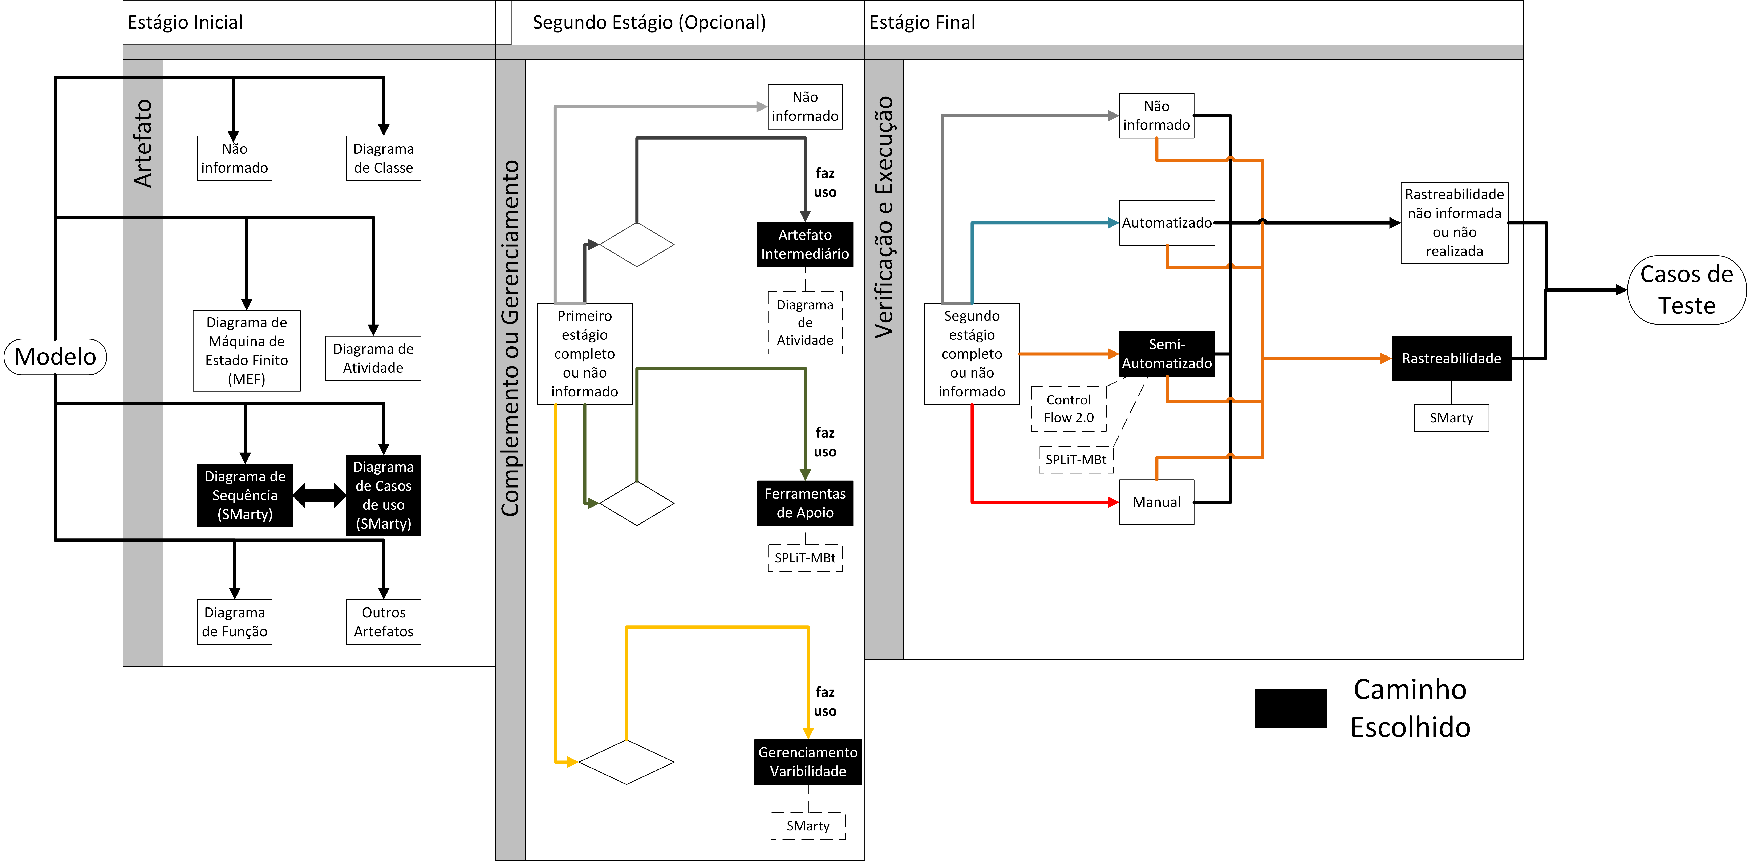
\includegraphics[scale=0.80]{roadmapcaminho2.pdf}
		\caption{Processo de geração de sequência de teste com \textit{SMartyTesting} (instância da \ref{fig:roadmap} )}
		\label{fig:roadmapcaminho}
	\end{figure}
\end{landscape}


\begin{figure}[h!]
	\centering
	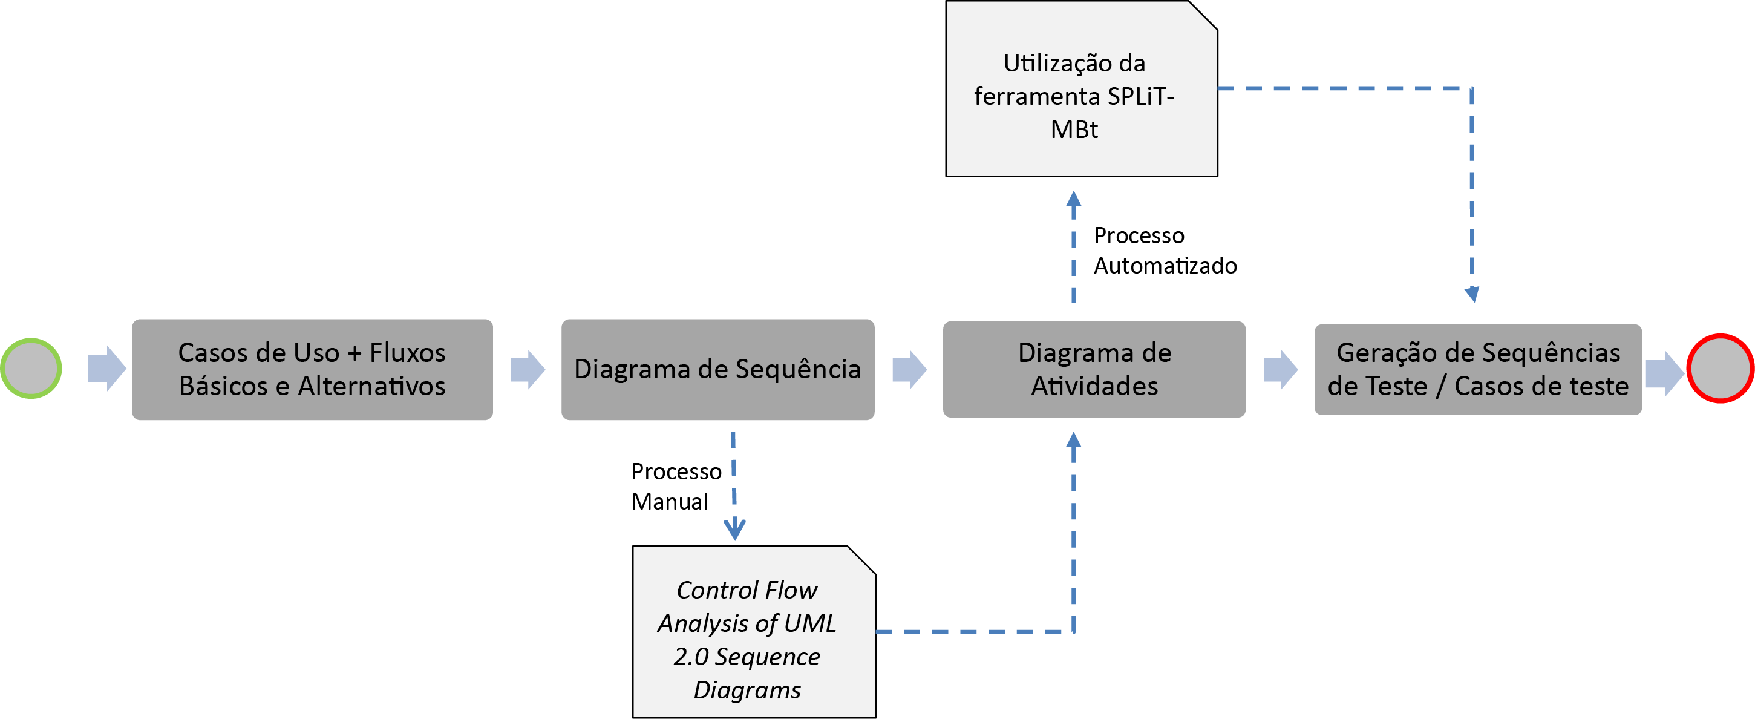
\includegraphics[scale=0.50]{ciclo_pesquisafinal.pdf}
	\caption{Passos para a geração de sequências de teste usando \textit{SMartyTesting}}
	\label{fig:ciclopesquisafinal}
\end{figure}


\subsection{Conversão de Diagramas de Sequência para Diagramas de Atividades}
\label{cap3subsec:conversaosequencia}


A conversão de diagramas de sequência para diagramas de atividades foi uma opção restritiva pelo fato de a ferramenta SPLiT-MBt ter como entrada diagramas de atividades. Embora também seja um diagrama de comunicação, o diagrama de atividades demonstra mais o fluxo de controle de uma atividade para outra, assim como a concorrência das atividades. Pode-se dizer que, enquanto o diagrama de sequência está mais próximo de métodos e do código-fonte, o diagrama de atividades está mais próximo dos casos de uso em termos de abstração.

Os dois diagramas são equivalentes quando se trata de elementos de representação, um exemplo é que em um diagrama de sequência, uma condicional de decisão pode ser representada por um diagrama de atividades, assim como quando um método, em um diagrama de sequência envia uma mensagem concorrente, criando uma bifurcação (\textit{fork}). 

Baseado no estudo de \citet{garousi2005control}, outro fator para a utilização de conversão de sequência para atividade é que não se corre o risco de perder propriedades no mapeamento, mantendo as características de variabilidades que foram estendidas no diagrama de sequência. Porém, é necessária uma validação desse mapeamento, o que foi feito por \citet{swain2010test}, sendo portanto, uma oportunidade para validação também com \textit{SMartyTesting}.

Por esses fatores é que se optou pela conversão de diagramas de sequência para atividades, aproveitando a validação da abordagem em uma ferramenta já desenvolvida SPLiT-MBt, que tem suporte à variabilidade, enquadrando-se no escopo deste trabalho.

A proposta de \citet{garousi2005control} consiste de uma metodologia de análise de fluxo de controle baseada em diagramas de sequência (DS) da UML 2.0. Essa técnica pode ser usada durante o ciclo de desenvolvimento e em outras abordagens de teste que façam compreensão e execução de modelos. Entre muitas aplicações, essa técnica pode ser usada em sistemas baseados em DS. 

Com base nos diagramas de atividades bem definidos, a proposta \textit{Control Flow Analysis of UML 2.0 Sequence Diagrams} (CCFG) \cite{garousi2005control} apresenta um metamodelo do diagrama de atividades estendido (\ref{fig:mapeamento2}), para apoiar a análise de fluxo de controle dos diagramas de sequência. Assim, pode-se definir um mapeamento baseado em \textit{Object Constraint Language} (OCL) \cite{warmer2003object} que é uma linguagem declarativa para descrever as regras que se aplicam aos modelos UML.

\begin{figure}[h!]
	\centering
	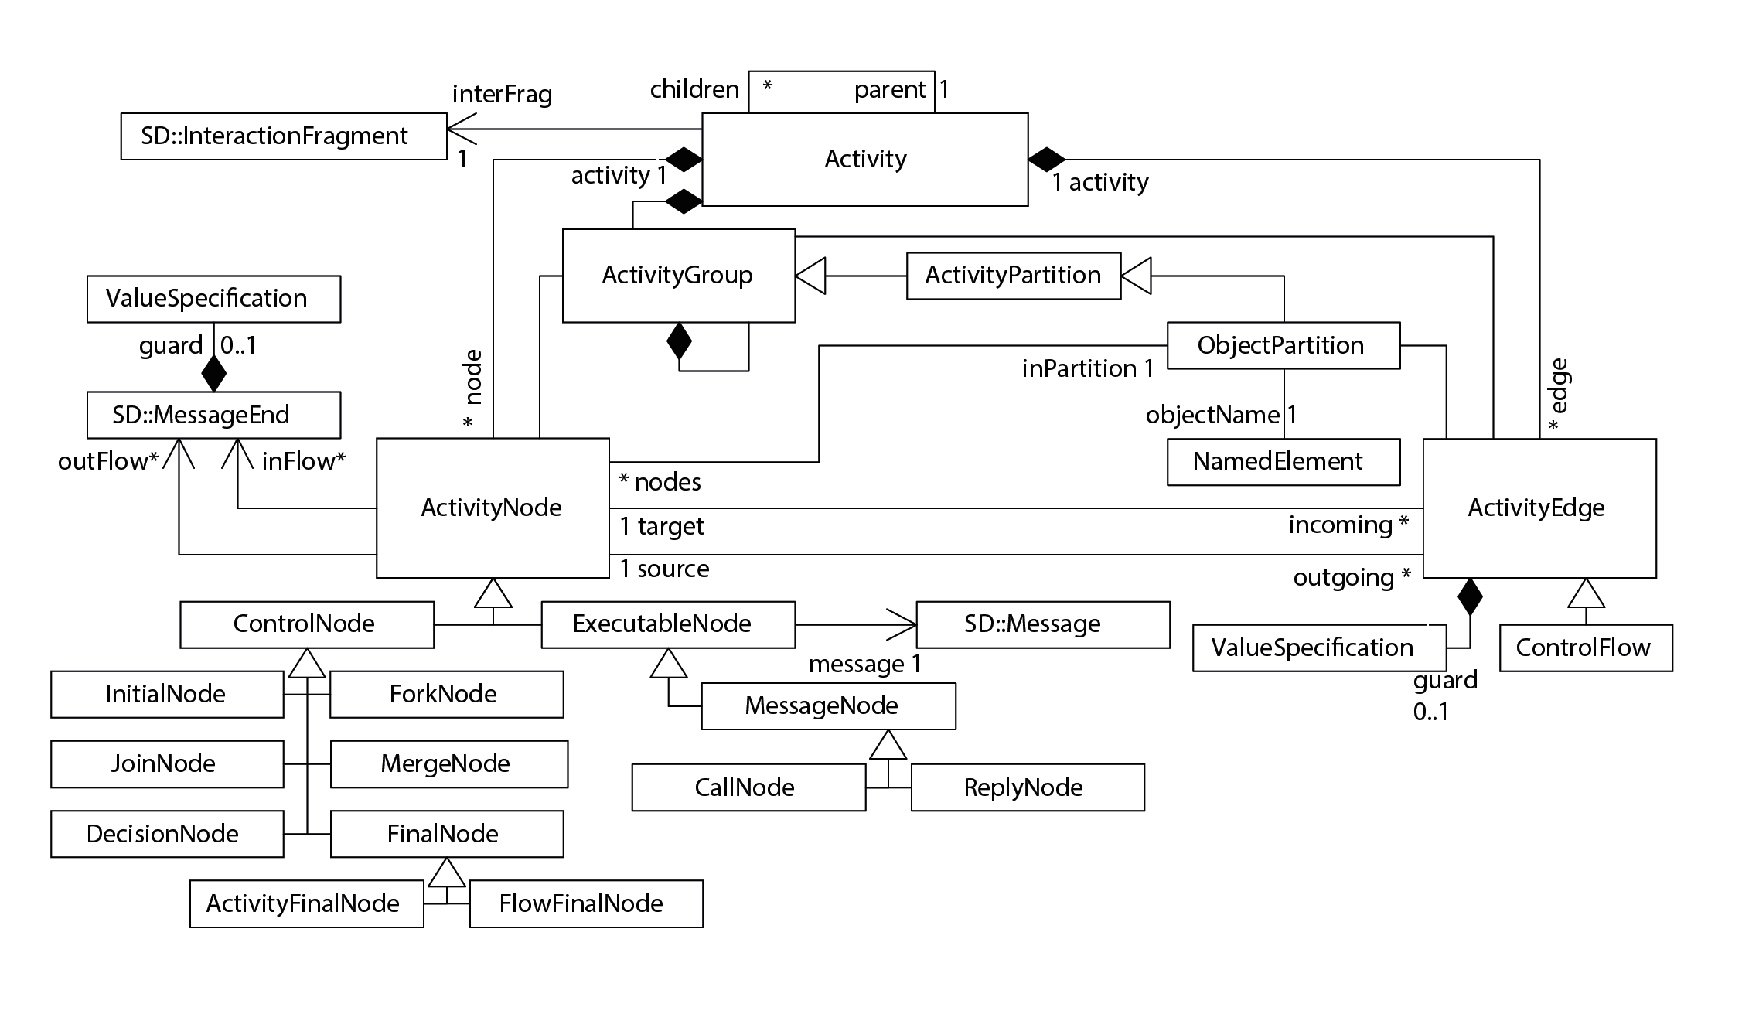
\includegraphics[scale=0.50]{atividade_metamodelo.pdf}
	\caption{Control Flow Analysis of UML 2.0 Sequence Diagrams metamodel (Diagramas de Atividades estendido) \cite{garousi2005control}}
	\label{fig:mapeamento2}
\end{figure}

A aplicação de OCL é realizada formalmente e verificável com regras de consistência entre um DS e um CCFG (diagramas de atividades estendido), em que CCFG possui todas as classes e associações necessárias, assim como suporte aos caminhos de fluxo de controle simultâneos (concorrência), que são uma generalização do conceito convencional de caminho de fluxo de controle \cite{garousi2005control}. 

O mapeamento consiste da utilização de um metamodelo DS (\ref{fig:mapeamento3}) e um conjunto de regras que deve ser utilizado na conversão, em que o metamodelo CCFG (\ref{fig:mapeamento2}) é considerado como validador.

\begin{figure}[h!]
	\centering
	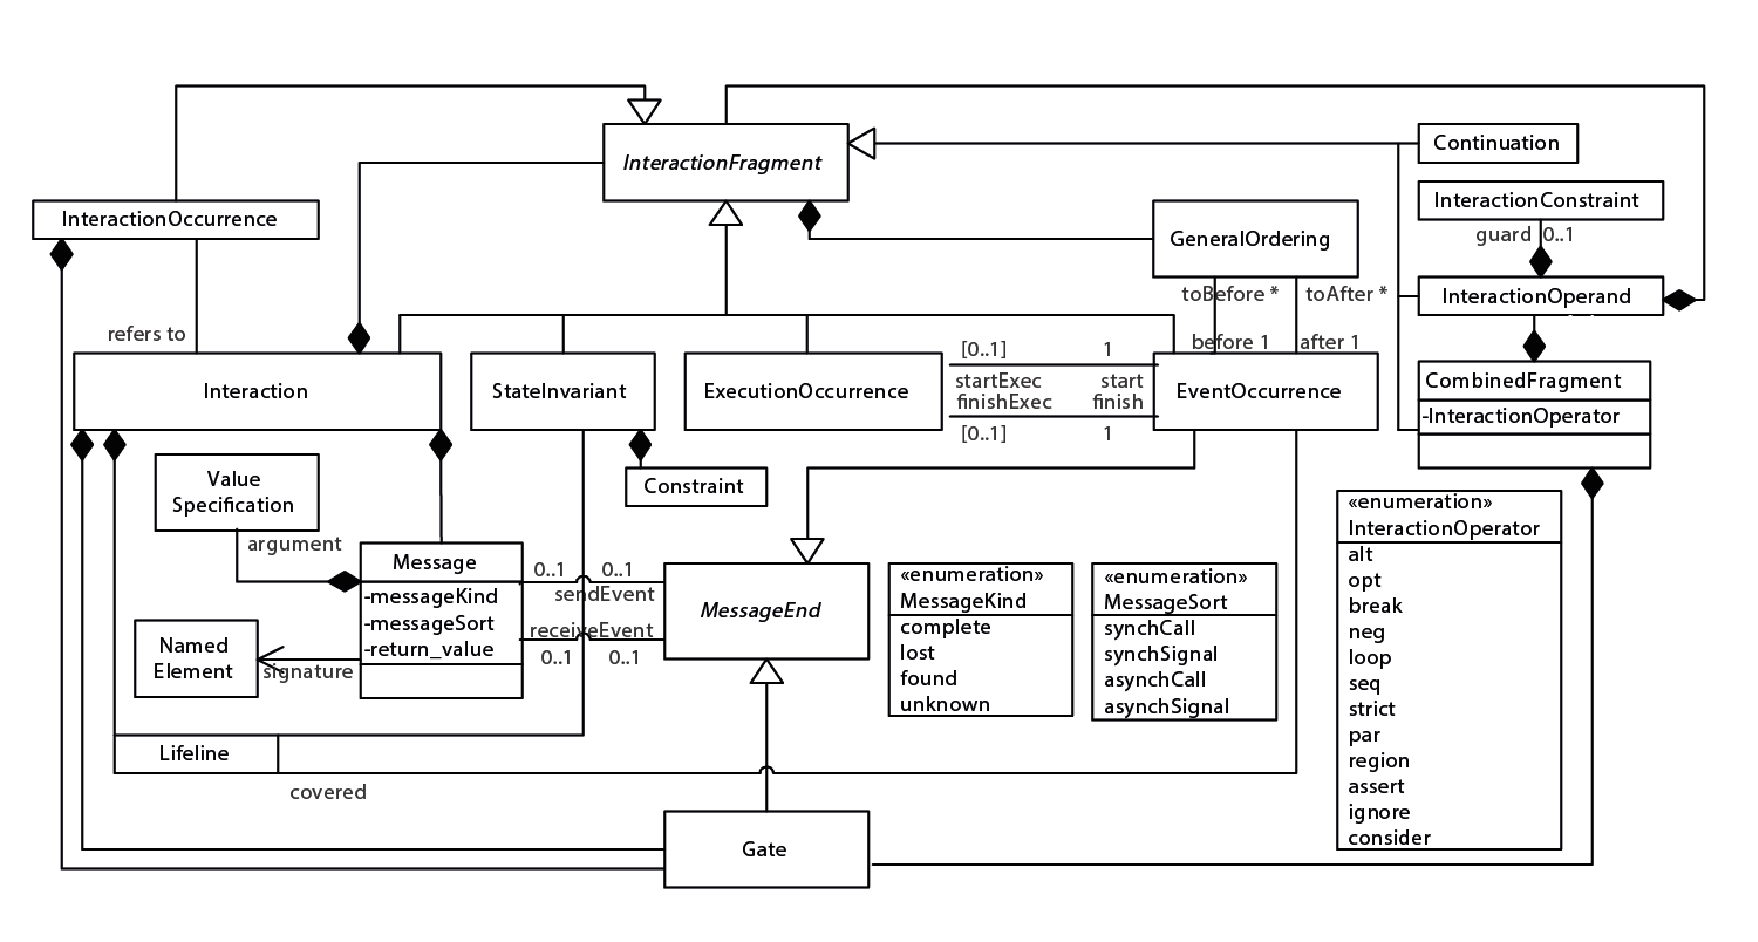
\includegraphics[scale=0.50]{sequencia_metamodelo.pdf}
	\caption{Metamodelo de diagramas de sequência UML \cite{garousi2005control}}
	\label{fig:mapeamento3}
\end{figure}

Como exemplo, tem-se diagramas de sequência (\ref{fig:mapeamento1}) que aparenta mensagens assíncronas. Para realizar o mapeamento para atividades (CCFG) foi utilizado um conjunto de regras criadas a partir dos metamodelos \cite{garousi2005control}. As regras são apresentadas na \ref{tab:regrasmapeamento}. Com isso, o processo de mapeamento deu origem ao diagrama de atividades apresentado na \ref{fig:mapeamento4}.   

\begin{figure}[h!]
	\centering
	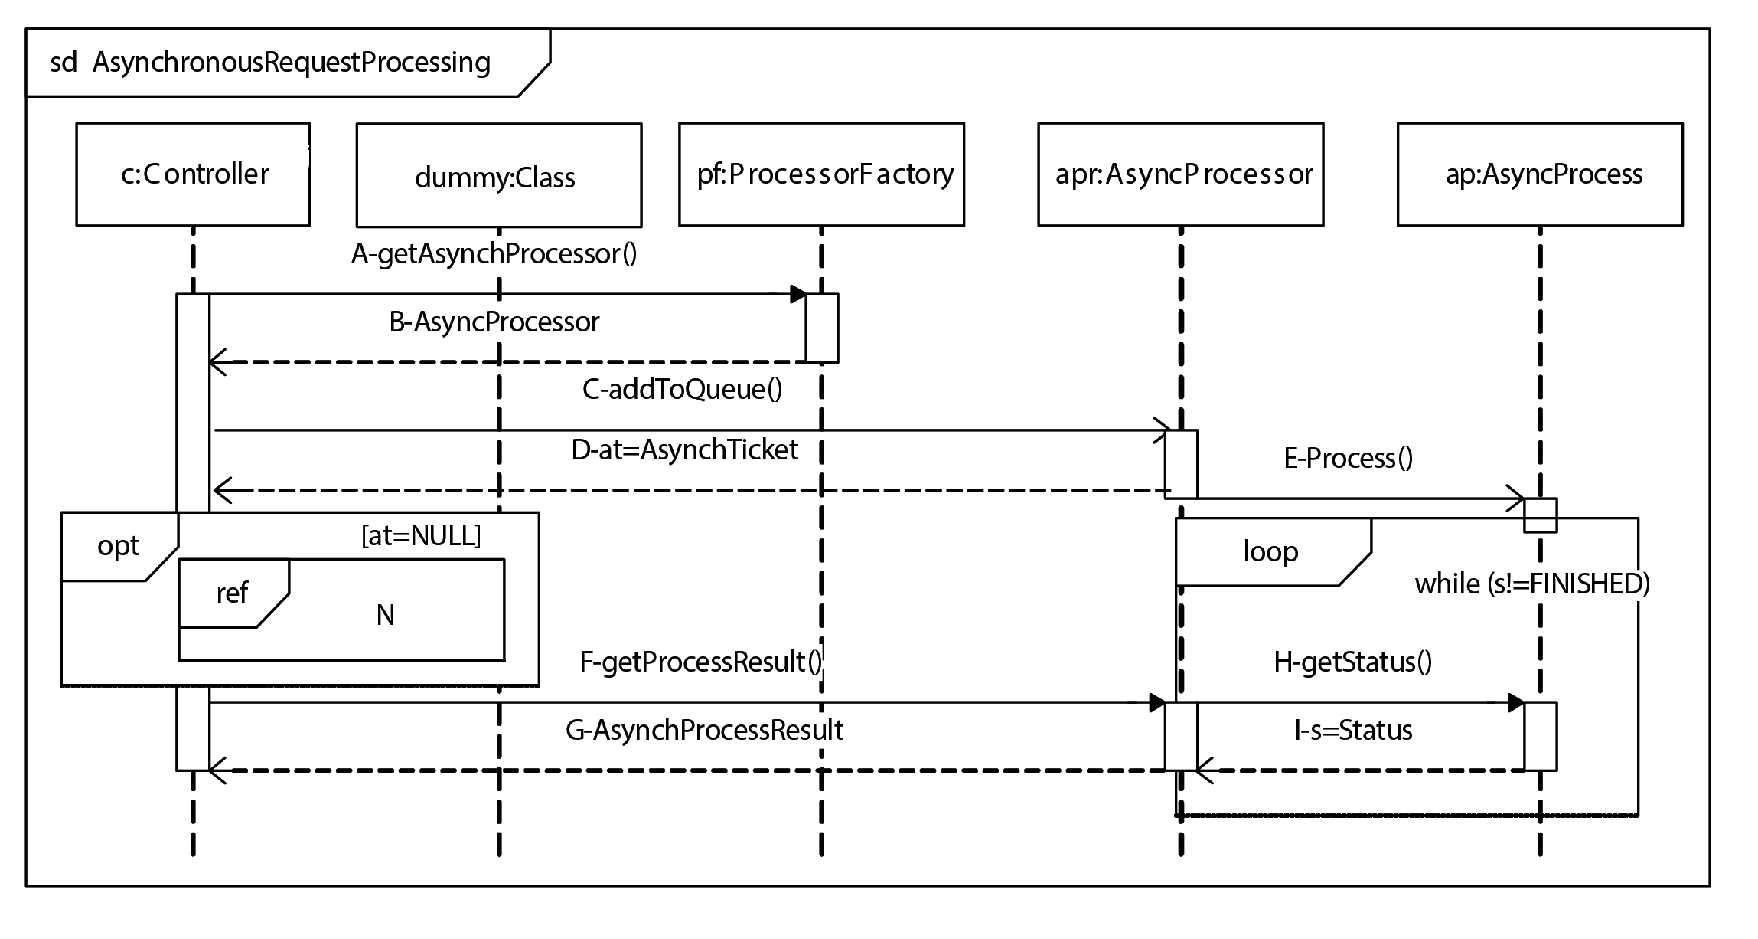
\includegraphics[scale=0.50]{diag_sequencia.pdf}
	\caption{Um diagrama de sequência com mensagens assíncronas \cite{garousi2005control}}
	\label{fig:mapeamento1}
\end{figure}


\begin{table}[h!]
	\centering
	\caption{Regras utilizadas para a conversão de DS para DA \cite{garousi2005control}}
	\label{tab:regrasmapeamento}
	\begin{tabular}{c|l|l}
		\hline
		\textbf{N°} & \multicolumn{1}{c|}{\textbf{Recurso do DS}} & \multicolumn{1}{c}{\textbf{Recurso do CCFG (Atividades)}} \\ \hline
		1 & Interaction & Activity \\ \hline
		2 & First message end & \begin{tabular}[c]{@{}l@{}}Flow between InitialNode\\ and first control node\end{tabular} \\ \hline
		3 & SynchCall/SynchSignal & CallNode \\ \hline
		4 & AsynchCall or AsynchSignal & \begin{tabular}[c]{@{}l@{}}(CallNode+ForkNode) or\\ ReplyNode\end{tabular} \\ \hline
		5 & \begin{tabular}[c]{@{}l@{}}Message SendEvent and\\ ReceiveEvent\end{tabular} & ControlFlow \\ \hline
		6 & Lifeline & ObjectPartition \\ \hline
		7 & par CombinedFragment & ForkNode \\ \hline
		8 & loop CombinedFragment & DecisionNode \\ \hline
		9 & alt/opt CombinedFragment & DecisionNode \\ \hline
		10 & break CombinedFragment & ActivityEdge \\ \hline
		11 & Last message ends & \begin{tabular}[c]{@{}l@{}}Flow between end control\\ nodes and FinalNode\end{tabular} \\ \hline
		12 & InteractionOccurrence & Control Flow across CCFGs \\ \hline
		13 & Polymorphic message & DecisionNode \\ \hline
		14 & Nested InteractionFragmen & Nested CCFGs \\ \hline
	\end{tabular}
\end{table}


\begin{figure}[H]
	\centering
	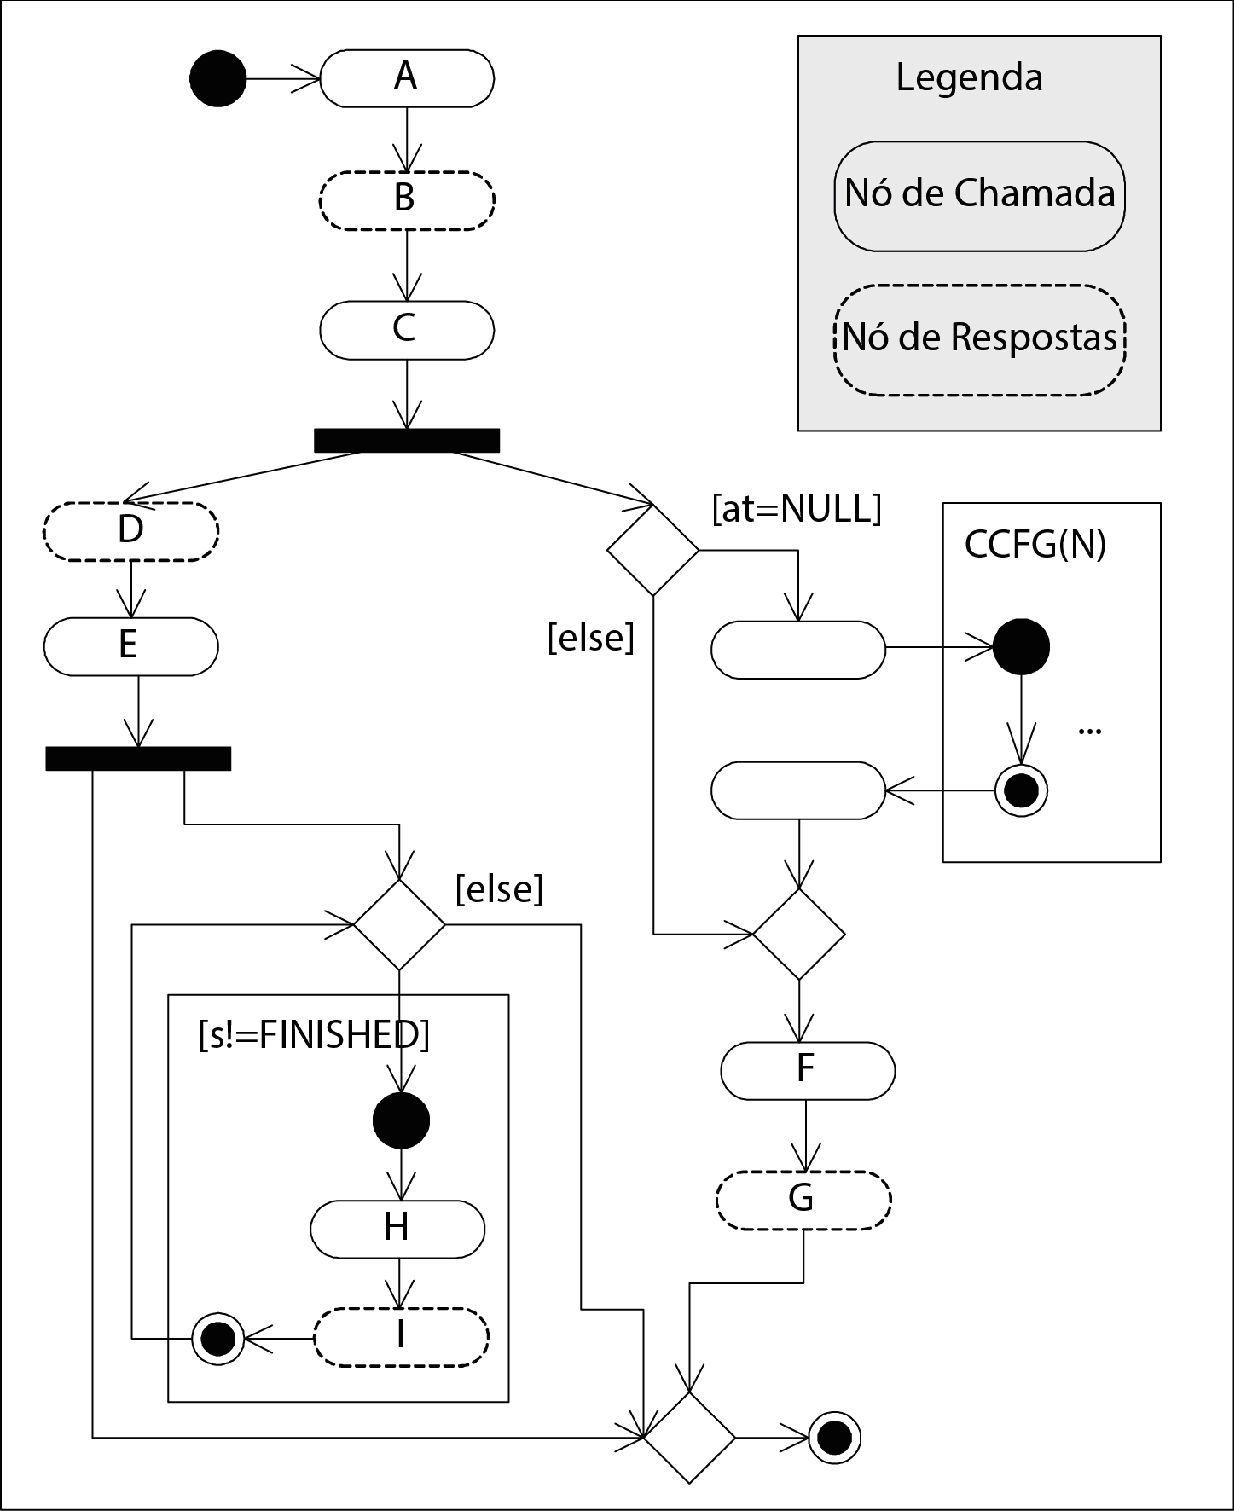
\includegraphics[scale=0.40]{sequencia_result_map.pdf}
	\caption{Resultado do mapeamento do DS da \ref{fig:mapeamento1}. Traduzido de \citet{garousi2005control}}
	\label{fig:mapeamento4}
\end{figure}

Para a validação da abordagem \textit{SMartyTesting} foi realizada a conversão manual dos DSs para DAs utilizando a ferramenta \textit{Astah professional 6}\footnote[1]{Disponível em: http://astah.net/download - Acessado em 20/10/2019}. Ao final da criação dos diagramas, os mesmos foram exportados com extensão XML, para serem utilizados na segunda etapa por SPLiT-MBt.

  
\subsection{Ferramenta Utilizada}
\label{cap3sec:ferramenta_utilizada_split}


SPLiT-MBt faz o uso do método de geração HSI. A razão para a escolha desse método se deve ao fato de ser um dos métodos menos restritivos em relação às propriedades que as MEFs devem ter. Por exemplo, o HSI é capaz de interpretar MEFs completas e parciais \cite{petrenko1994nondeterministic}. 

Além disso, o método HSI permite cobertura total de falhas existentes e gera sequências de teste menores que outros métodos, o que contribui para a otimização do processo de teste. Esses fatores são muito relevantes no contexto da LPS, porque quanto maior o número de \textit{features} de uma LPS, maior é o número de casos de teste necessários para testar produtos da LPS \cite{engstrom2011software}.

Como houve necessidade de se estender a abordagem por causa da variabilidade, para gerar sequências de teste a partir de uma versão estendida do HSI, foi necessário aplicar o método considerando as informações de variabilidade presentes no MEF. 

A SPLiT-MBt aceita, inicialmente, um arquivo de entrada em formato \textit{eXtensible Markup Language} (XML), faz a leitura do arquivo e valida todos os requisitos de entrada do artefato. Caso esteja correto, monta-se a estrutura e, assim que o usuário clica na opção de geração, SPLiT-MBt converte o DA em MEF em tempo de execução e realiza o processo de geração de sequências de teste.


\section{Especificação da Abordagem \textit{SMartyTesting}}
\label{cap3sec:especificacao_smarty}
Nesta seção é apresentado cada passo da abordagem \textit{SMartyTesting}. Neste trabalho, parte-se do princípio de que a modelagem de casos de uso tenha dado origem aos diagramas de sequência.

\subsection{Etapa 1 - Mapeamento de Diagramas de Sequência para Diagramas de Atividades}
\label{cap3subsec:etapa1}

Nesta primeira etapa foi realizado o mapeamento dos diagramas de sequência (DS) para o de atividades estendido (DA). Para tanto, foi usada a LPS AGM. A etapa 1 é ilustrada na \ref{fig:SM_etapa1}. 

\begin{figure}[h!]
	\centering
	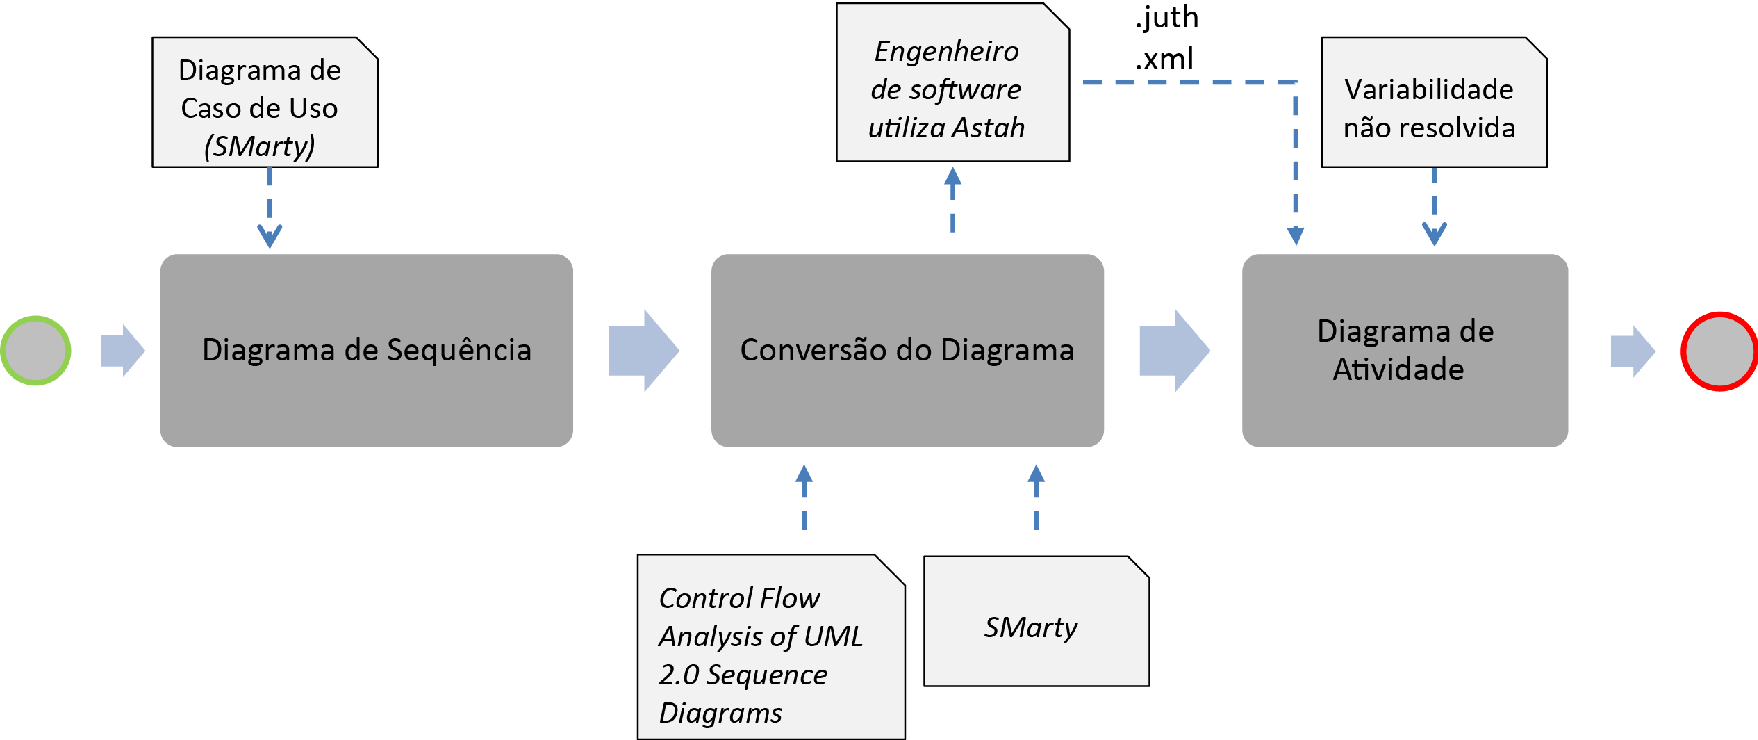
\includegraphics[scale=0.50]{etapa1_ds_to_da.pdf}
	\caption{Ciclo da etapa 1}
	\label{fig:SM_etapa1}
\end{figure}


O DS foi modelado considerando a abordagem \textit{SMarty} utilizando a ferramenta \textit{Cameo Enterprise Architecture} versão 19 \footnote{\url{https://www.nomagic.com/products/cameo-enterprise-architecture}}. Depois de modelado o diagrama de sequência e todas as suas propriedades (\ref{fig:exemploDS}), o engenheiro de software deverá construir um novo diagrama de atividades, porém levando em consideração as regras da \ref{tab:regrasmapeamento} e as propriedades do diagrama de sequência criado.


\begin{figure}[h!]
	\centering
	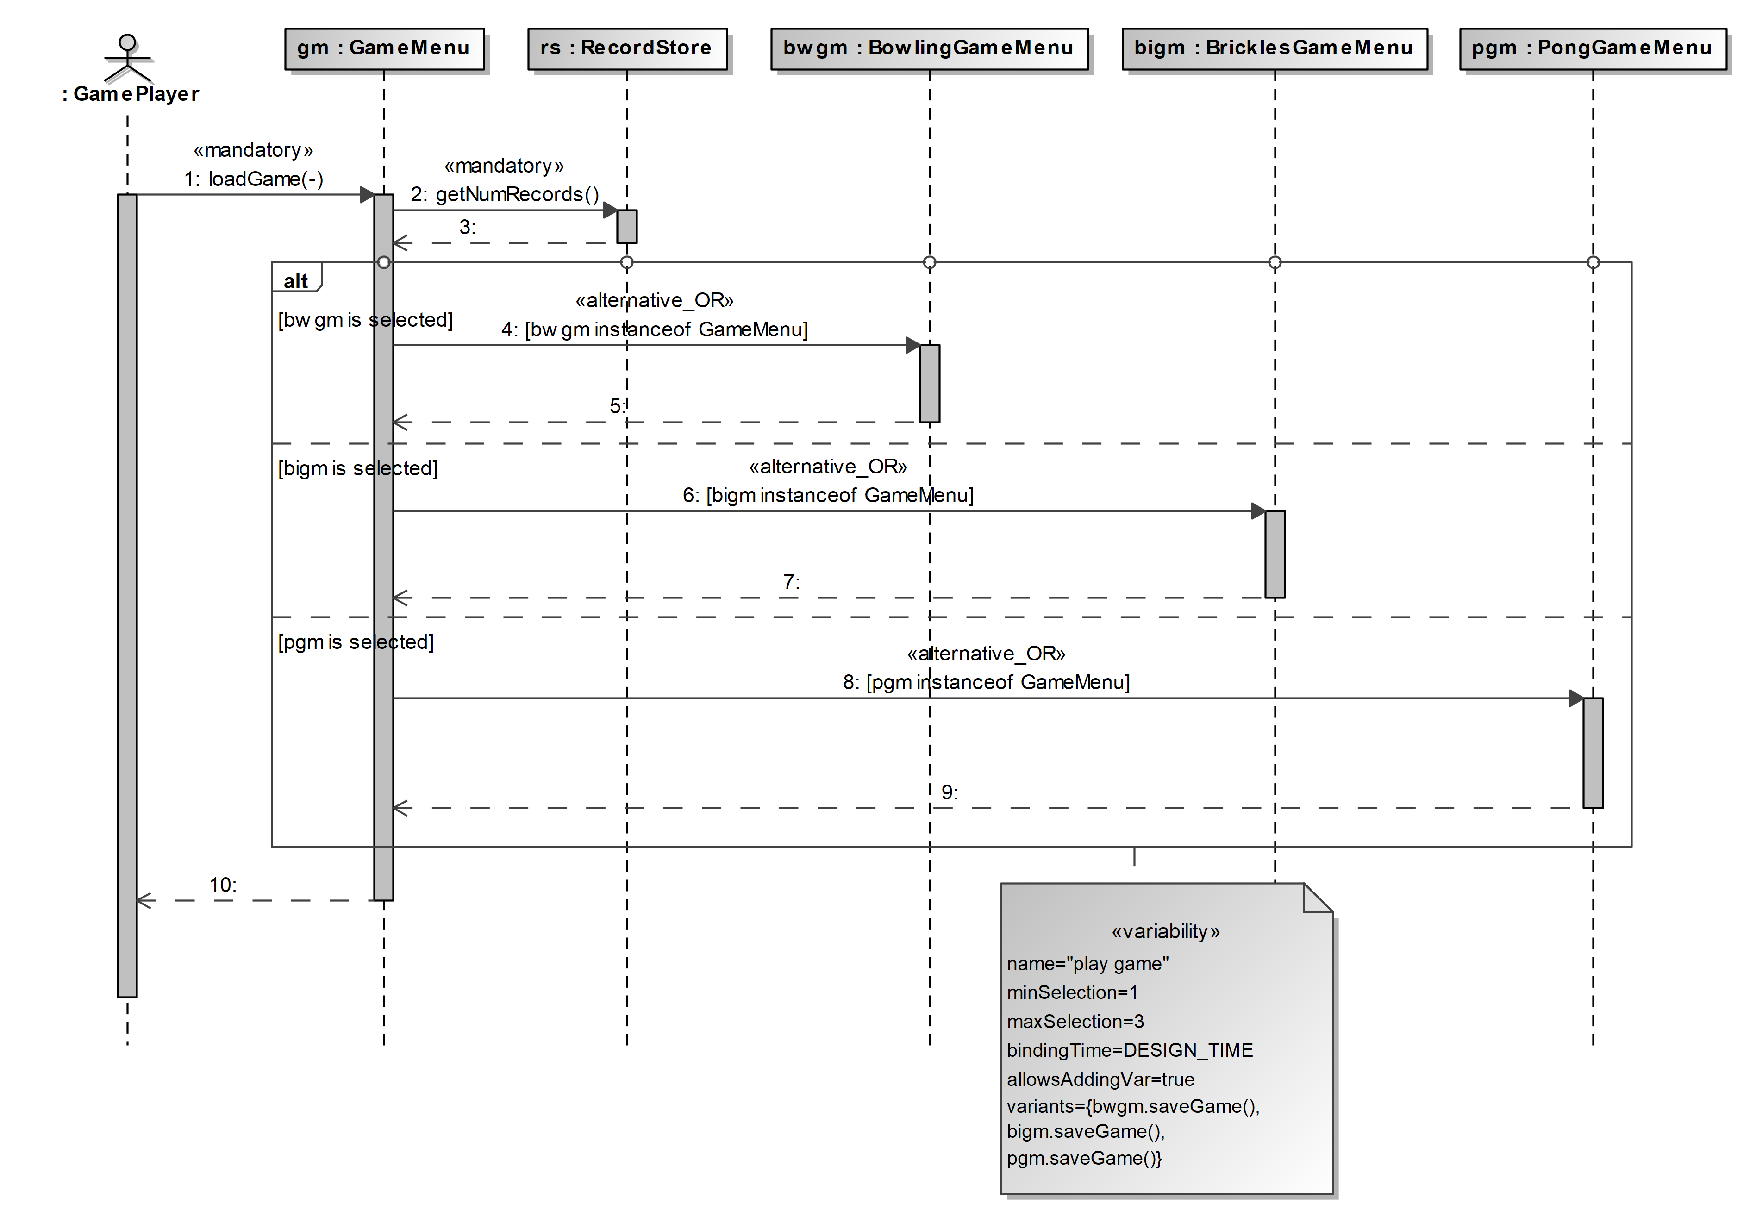
\includegraphics[scale=0.47]{exemploDS.pdf}
	\caption{Diagramas de sequência ilustrando o caso de uso \textit{game menu} da AGM}
	\label{fig:exemploDS}
\end{figure}

Neste trabalho utilizou-se outra ferramenta (IDE) de modelagem para a criação do modelo convertido de DS para DA, a ferramenta utilizada foi a \textit{Astah} versão 6. Optou-se por essa versão a fim de demonstrar que mesmo com IDEs diferentes para modelagem, pode-se chegar ao mesmo resultado esperado.

A criação do DA deve levar em consideração o uso das regras de mapeamento contidas na \ref{tab:regrasmapeamento}, as propriedades de variabilidade são mantidas sem a resolução, a fim de serem transportadas às sequências de teste para serem reutilizadas. A \ref{fig:exemploDA} apresenta o resultado da conversão do DS da \ref{fig:exemploDS}.

Na execução da construção do DA deve-se levar em consideração os requisitos necessários que serão utilizados na Etapa 2. O arquivo do artefato modelado deve ser exportado da ferramenta em formato XML, que é o formato de entrada suportado por SPLiT-MBt.

\begin{figure}[H]
	\centering
	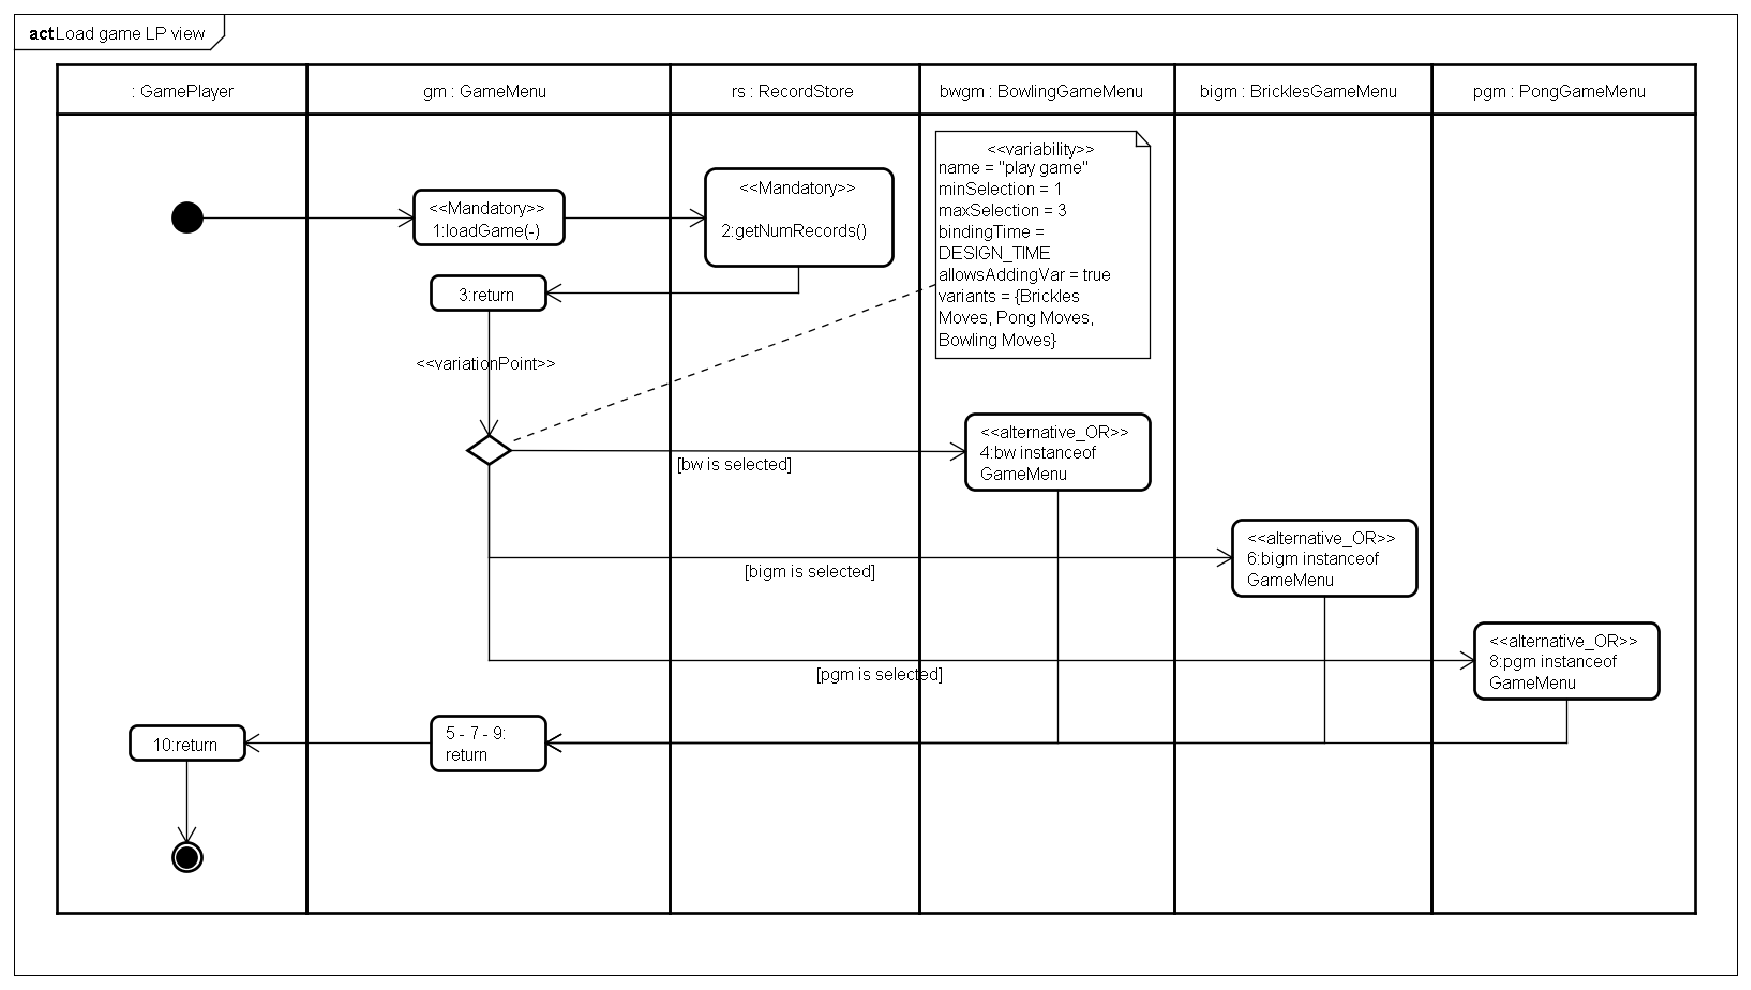
\includegraphics[scale=0.55]{exemploDA.pdf}
	\caption{Diagramas de atividades resultante do mapeamento do DS da \ref{fig:exemploDS}}
	\label{fig:exemploDA}
\end{figure}

Para a utilização do arquivo do artefato de DA, antes da exportação pela IDE, devem ser levadas em consideração algumas características. Uma delas é a parametrização das transições do DA, necessárias para utilização na ferramenta SPLiT-MBt. Deve ser levado em consideração também o estereótipo da atividade que está sendo modelada fazendo uso de \textit{SMarty}.

Esses parâmetros são informações referentes às transições no DA. Assim, tem-se a transição da atividade, na que está contida a \textit{tag} identificando qual é a ação (\textit{TDaction}) e o resultado esperado (\textit{TDexpectedResult}) e, por fim, os valores (\textit{Values}) que são adicionados conforme as especificações do DA. A \ref{fig:exemploTAG} apresenta uma visão dessa configuração necessária. 

\begin{figure}[H]
	%\centering
	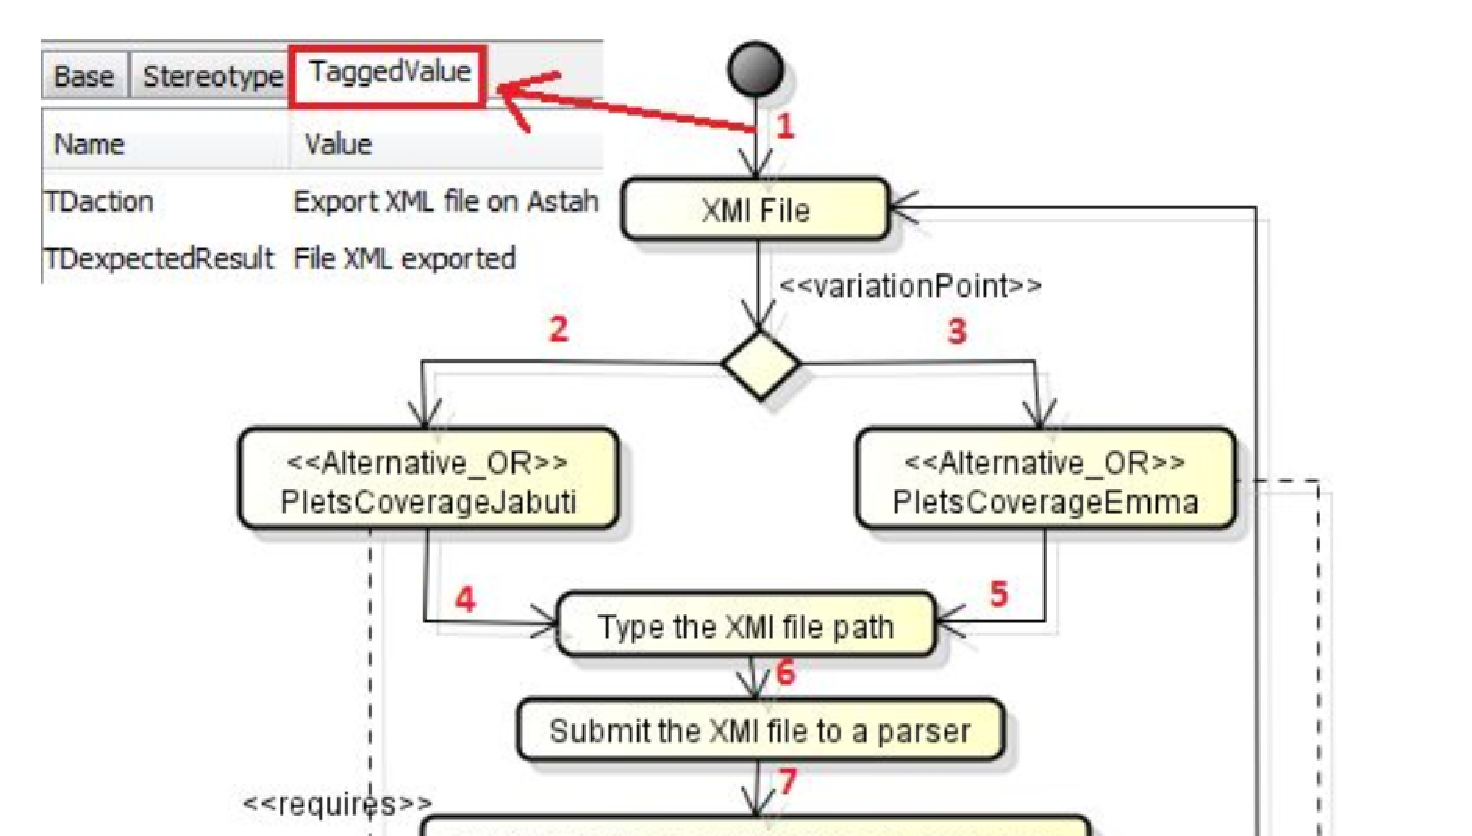
\includegraphics[scale=0.50]{exemploTAG.pdf}
	\caption{Exemplificação da parametrização dos \textit{controlflows} de um diagrama de atividades usando SPLiT-MBt \cite{costa2016split}}
	\label{fig:exemploTAG}
\end{figure}

Seguindo essa parametrização necessária, a \ref{tab:valores_tag} apresenta todos os parâmetros das transições do DA resultante do mapeamento.


%\begin{landscape}
	\begin{table}[H]
	    \footnotesize
		\caption{Valores dos atributos de parametrização do DA para utilização em SPLiT-MBt}
		\label{tab:valores_tag}
		\begin{tabular}{l|l|l}
			\hline
			\textbf{Transição das Atividades} & \textbf{Tags} & \textbf{Valores} \\ \hline
			\begin{tabular}[c]{@{}l@{}}1- Estágio Inicial \\ para LoadGame\end{tabular} & \begin{tabular}[c]{@{}l@{}}TDaction\\ TDexpectedResult\end{tabular} & \begin{tabular}[c]{@{}l@{}}- Game Player faz o carregamento do jogo\\ - Jogo carrega\end{tabular} \\ \hline
			\begin{tabular}[c]{@{}l@{}}2- LoadGame \\ para getNumRecords\end{tabular} & \begin{tabular}[c]{@{}l@{}}TDaction\\ TDexpectedResult\end{tabular} & \begin{tabular}[c]{@{}l@{}}- Game menu faz acesso ao dados de pontuação\\ - Consegue acesso ao dados de pontuação\end{tabular} \\ \hline
			\begin{tabular}[c]{@{}l@{}}3- getNumRecords \\ para return\end{tabular} & \begin{tabular}[c]{@{}l@{}}TDaction\\ TDexpectedResult\end{tabular} & \begin{tabular}[c]{@{}l@{}}- recordStore retorna os dados\\ - Dados de pontuação são retornados\end{tabular} \\ \hline
			\begin{tabular}[c]{@{}l@{}}4- Decision node para \\ bw instanceof GameMenu\end{tabular} & \begin{tabular}[c]{@{}l@{}}TDaction\\ TDexpectedResult\end{tabular} & \begin{tabular}[c]{@{}l@{}}- Opção bw é selecionada\\ - Acesso aos recurso da opção bw\end{tabular} \\ \hline
			5- return & \begin{tabular}[c]{@{}l@{}}TDaction\\ TDexpectedResult\end{tabular} & \begin{tabular}[c]{@{}l@{}}- Retorno da opção bw\\ - Retorne ao menu de opções\end{tabular} \\ \hline
			\begin{tabular}[c]{@{}l@{}}6- Decision node para \\ bigm instanceof GameMenu\end{tabular} & \begin{tabular}[c]{@{}l@{}}TDaction\\ TDexpectedResult\end{tabular} & \begin{tabular}[c]{@{}l@{}}- Opção bigm é selecionada\\ - Acesso aos recurso da opção bigm\end{tabular} \\ \hline
			7- return & \begin{tabular}[c]{@{}l@{}}TDaction\\ TDexpectedResult\end{tabular} & \begin{tabular}[c]{@{}l@{}}- Retorno da opção bigm\\ - Retorne ao menu de opções\end{tabular} \\ \hline
			\begin{tabular}[c]{@{}l@{}}8- Decision node para \\ pgm instanceof GameMenu\end{tabular} & \begin{tabular}[c]{@{}l@{}}TDaction\\ TDexpectedResult\end{tabular} & \begin{tabular}[c]{@{}l@{}}- Opção pgm é selecionada\\ - Acesso aos recurso da opção pgm\end{tabular} \\ \hline
			9- return & \begin{tabular}[c]{@{}l@{}}TDaction\\ TDexpectedResult\end{tabular} & \begin{tabular}[c]{@{}l@{}}- Retorno da opção pgm\\ - Retorne ao menu de opções\end{tabular} \\ \hline
			10- return & \begin{tabular}[c]{@{}l@{}}TDaction\\ TDexpectedResult\end{tabular} & \begin{tabular}[c]{@{}l@{}}- Retorno da informação ao Game Player\\ - Player recebe retorno da ação escolhida\end{tabular} \\ \hline
		\end{tabular}
	\end{table}
%\end{landscape}


\subsection{Etapa 2 - Geração de Sequências de Teste}
\label{cap3subsec:etapa2}

Na segunda etapa considera-se que o DS já tenha sido mapeado e convertido para DA, conforme o fluxo apresentado na \ref{fig:SM_etapa2}. Dado o mapeamento de conversão realizado faz-se a geração de sequências de casos de teste. 

\begin{figure}[H]
	\centering
	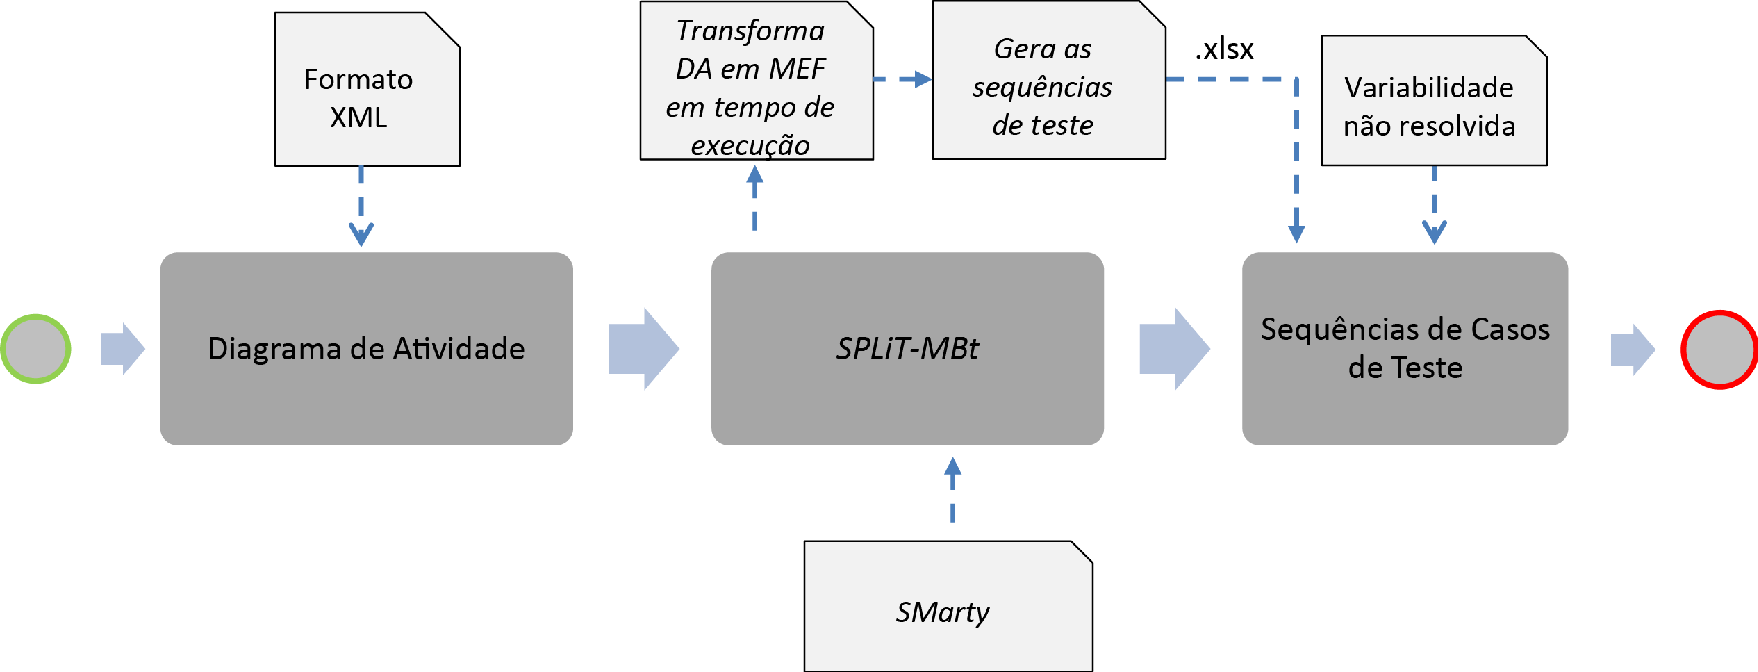
\includegraphics[scale=0.52]{etapa2_da_to_caso.pdf}
	\caption{Ciclo da etapa 2}
	\label{fig:SM_etapa2}
\end{figure}


De posse do arquivo XML gerado, inicia-se o carregamento do arquivo na ferramenta (\ref{fig:split_carregamento}). Após o arquivo ser carregado pela aplicação, faz-se a verificação da estrutura do arquivo XML (\ref{fig:split_validacao}).

\begin{figure}[h!]
	\centering
	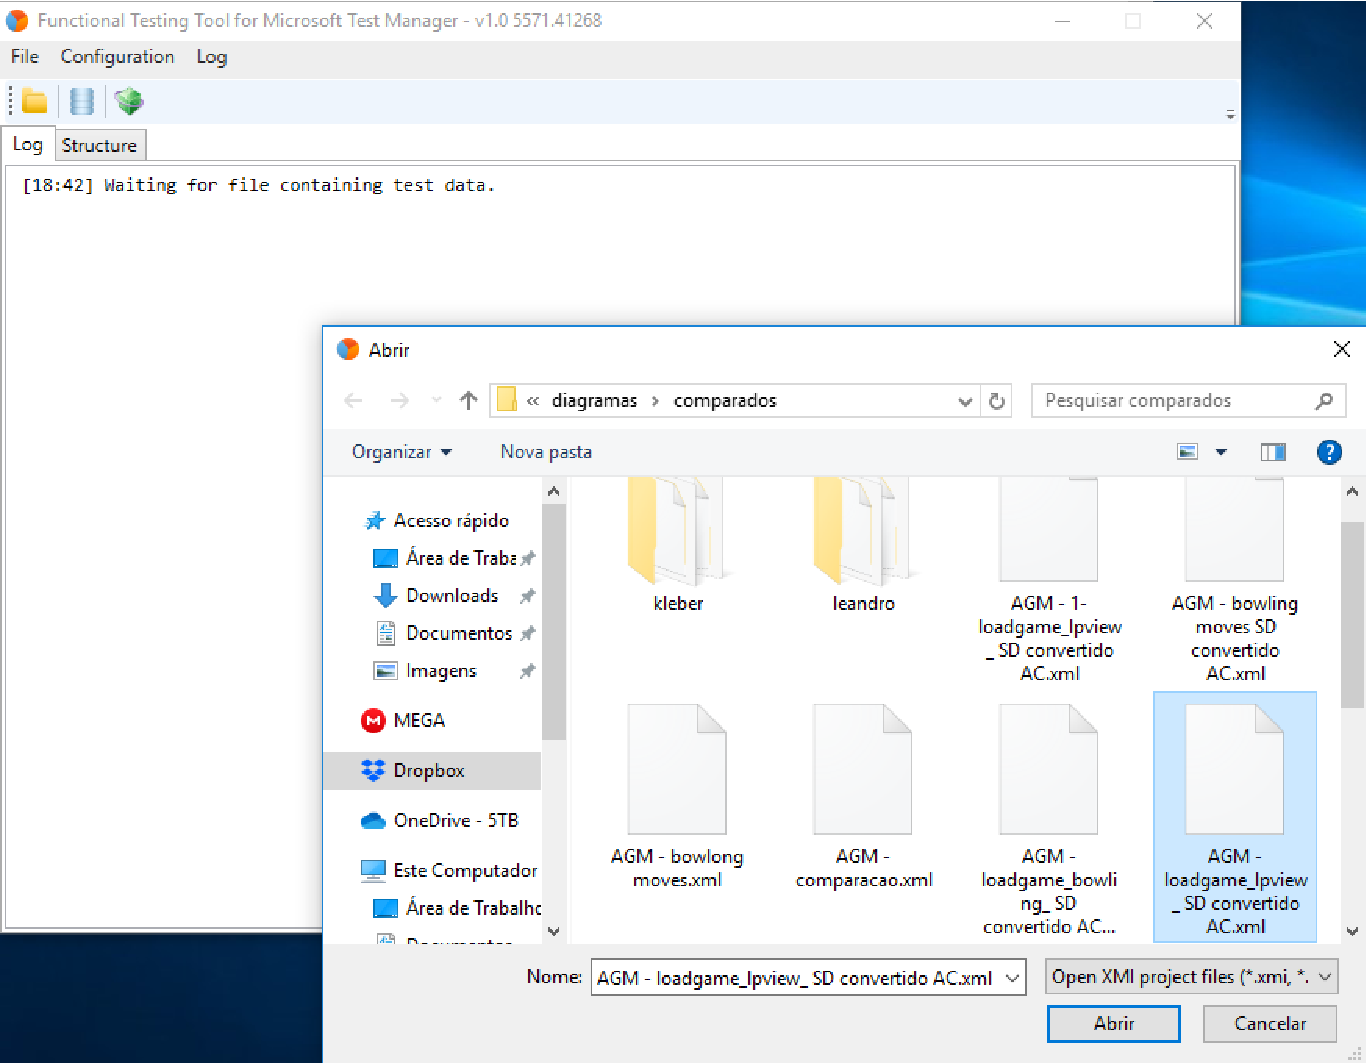
\includegraphics[scale=0.60]{splitcarregamento.pdf}
	\caption{Tela de carregamento de arquivo da ferramenta SPLiT-MBt}
	\label{fig:split_carregamento}
\end{figure}


\begin{figure}[h!]
	\centering
	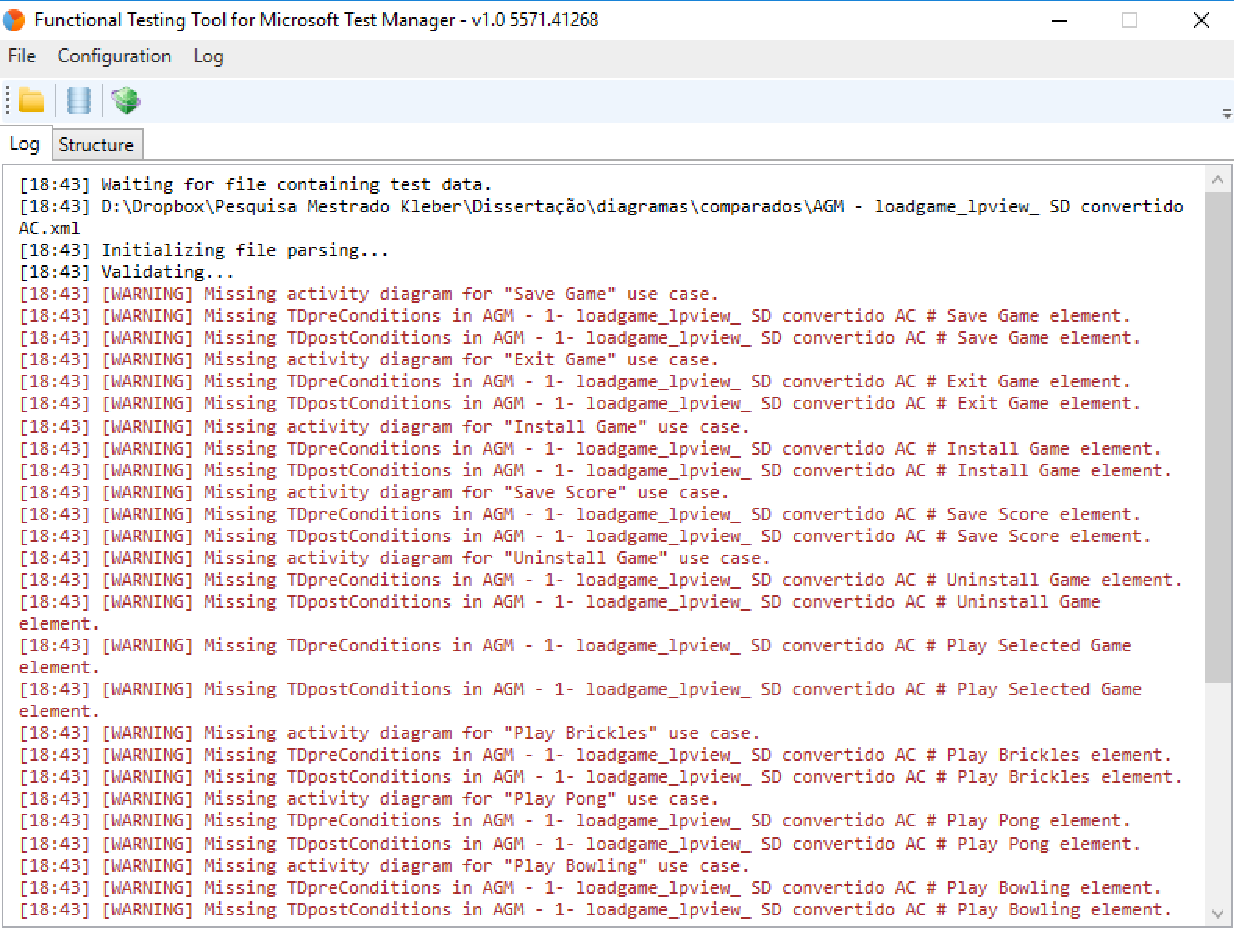
\includegraphics[scale=0.55]{splitvalidacao.pdf}
	\caption{Validação da estrutura do arquivo carregado pela SPLiT-MBt}
	\label{fig:split_validacao}
\end{figure}

Após a validação do arquivo que é carregado, pode ser observada a sua estrutura usando a própria ferramenta (\ref{fig:split_estrutura}), com isso pode-se realizar a geração de casos de teste e, quando não houver erros na geração, a mensagem de sucesso é apresentada (\ref{fig:split_gerado}).  

\begin{figure}[h!]
	\centering
	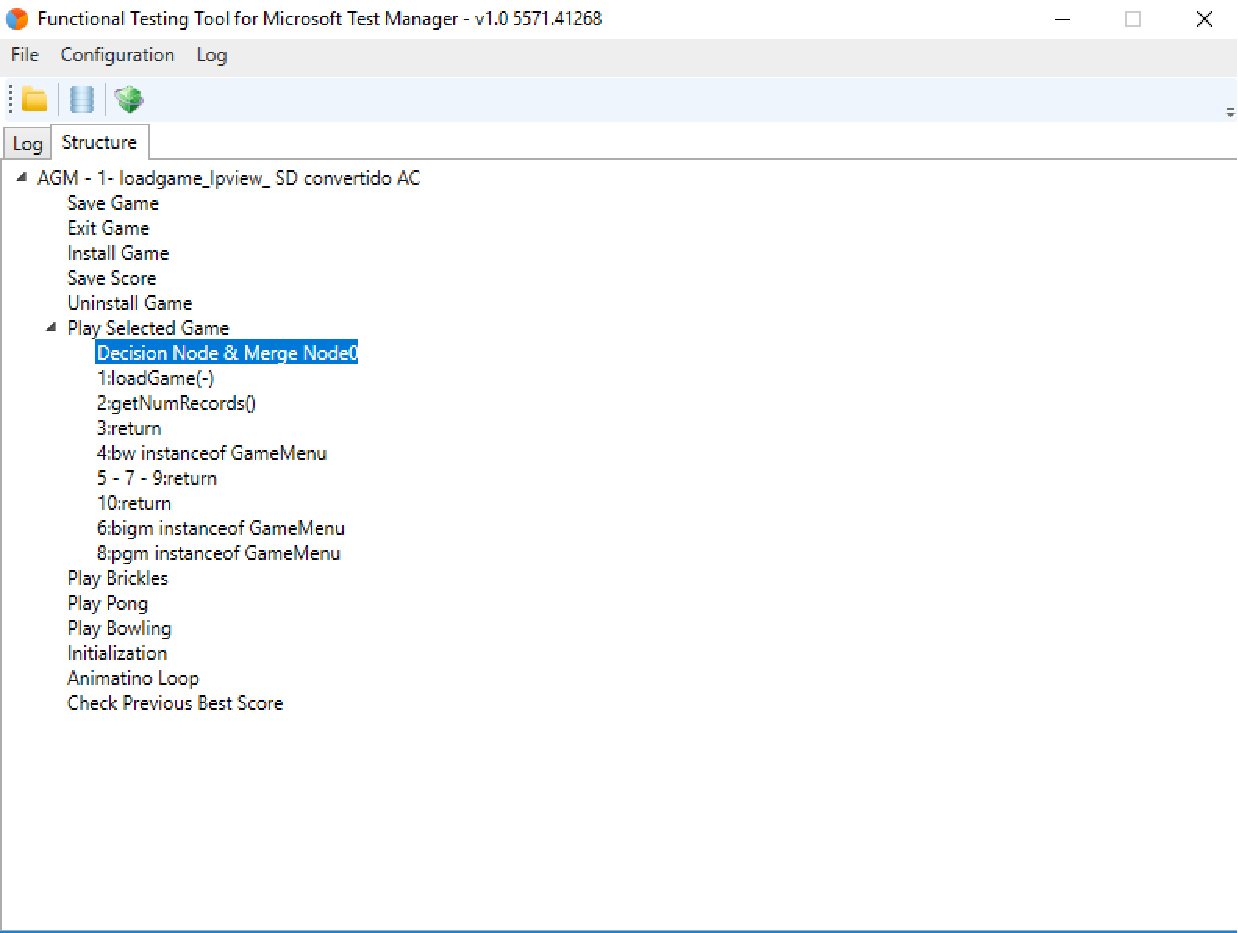
\includegraphics[scale=0.55]{splitestrutura.pdf}
	\caption{Apresentação da estrutura do arquivo XML}
	\label{fig:split_estrutura}
\end{figure}


No momento da geração a ferramenta faz a conversão do DA em MEFs estendidas para suportar variabilidade. Essa conversão é realizada em tempo de execução, assim, não há acesso a nenhum arquivo ou processo, tornando a execução um processo interno da ferramenta.

\begin{figure}[h!]
	\centering
	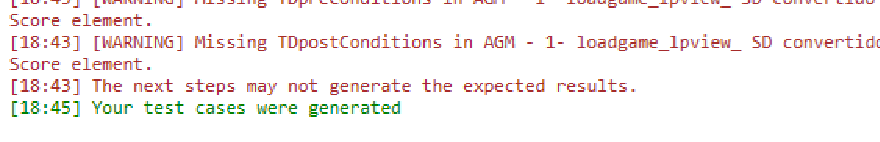
\includegraphics[scale=0.75]{splitgerado.pdf}
	\caption{Mensagem de sucesso na geração dos casos de teste}
	\label{fig:split_gerado}
\end{figure}

Após a geração, é possível exportar um arquivo XLSx, que é umdos formatos de extensão aceitados pelo Excel, (\ref{fig:split_casodeteste}) que pode ser utilizado em ferramentas de teste que fazem uso de \textit{scripts}.

\begin{figure}[h!]
	\centering
	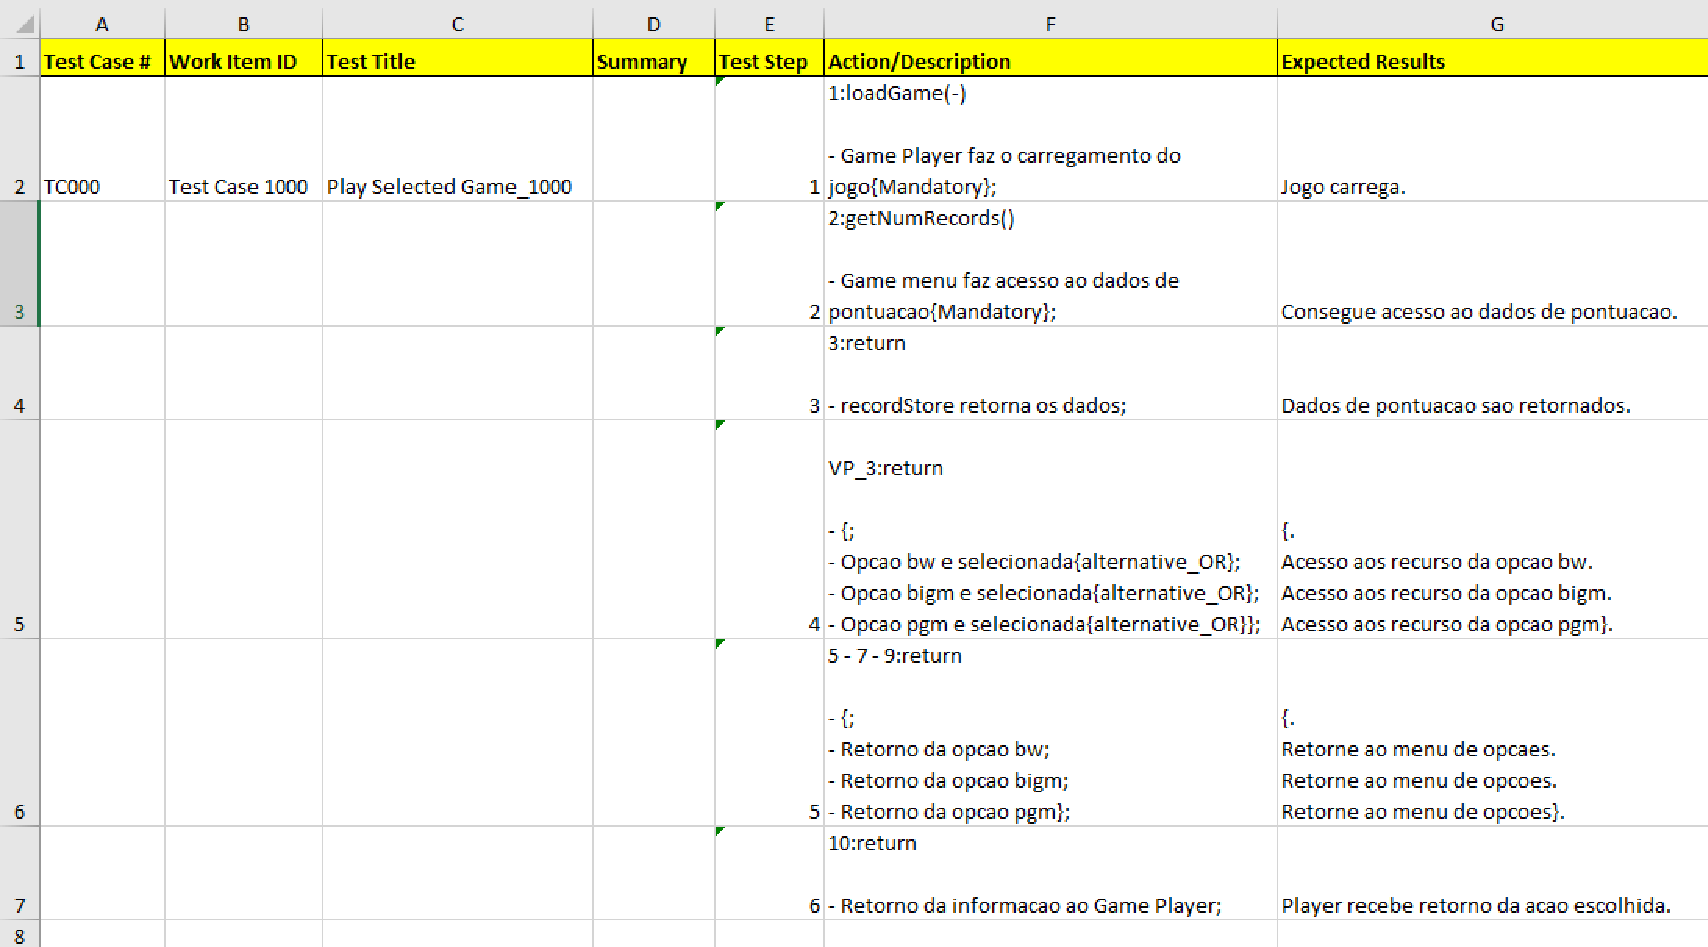
\includegraphics[scale=0.55]{splitcasodeteste.pdf}
	\caption{Arquivo XLSx com os casos de testes gerados}
	\label{fig:split_casodeteste}
\end{figure}
\newpage
\subsection{Resolução da Variabilidade}
\label{cap3subsec:solucao_variabilidade}

\textit{SMartyTesting} trata inicialmente a resolução da variabilidade no mesmo formato que SPLiT-MBt trata, onde as sequências de casos de teste são geradas contendo a variabilidade sem a resolução. Isso é importante quando se aborda a questão da reutilização, uma vez que quando novos produtos são gerados, a variabilidade pode sofrer alterações, ou haver mais pontos de variação. 

A viabilidade se torna desconhecida justamente por essa diferenciação que pode ser extensa, muitas instâncias e, quando se fala em reaproveitamento, a diferença pode sofrer um aumento e diferenciação, o que torna inviável a solução durante a modelagem.

Nesse caso, \textit{SMartyTesting} gera as sequências de teste com a variabilidade sem resolução, para que o engenheiro de software faça a tomada de decisão na engenharia de aplicação, analisando a melhor solução para a resolução da variabilidade contida.   


\subsection{Limitações de Uso da SPLiT-MBt}
\label{cap3subsec:limitacoes}

Por se estar utilizando ferramentas de apoio de terceiros, era previsto que limitações poderiam ser encontradas. Nesse caso, foram encontradas limitações em ambas as etapas.

Na primeira, com relação à utilização da notação \textit{SMarty} no mapeamento de conversão, pois \textit{Control Flow Analysis of UML 2.0 Sequence Diagrams} não cita soluções sobre variabilidade, embora, não sejam encontrados obstáculos sobre notações na utilização, a limitação ocorre somente por não ter uma regra explícita sobre notação de variabilidade.

Já na segunda etapa, envolvendo a aplicação de SPLiT-MBt, as limitações são mais significativas, embora não tenham influenciado nas validações. As limitações estão ligadas diretamente à estrutura do metamodelo do diagrama de atividades (\ref{fig:mapeamento2}).

SPLiT-MBt não fornece suporte a dois itens de \textit{ControlNode}, \textit{ForkNode} e \textit{JoinNode}, em testes com programação concorrente (atividades simultâneas). 

Outro ponto de limitação está ligado à continuidade de uma atividade após um \textit{DecisionNode} em que não são aceitas sub atividades a não ser que seja um estado de \textit{Merge}. Assim, considera-se isso uma não conformidade com sub-sistemas representados no artefato de entrada, um exemplo seria um \textit{InitialNode} vide (\ref{fig:mapeamento4}).  

Em um processo que não seja automatizado pode haver ameaças ao funcionamento, nesse caso a primeira etapa. Por esse motivo, é recomendado em trabalhos futuros a implementação e automatização de todos os processos do início ao fim do ciclo.

Pode-se considerar outra ameaça ao funcionamento da \textit{Control Flow Analysis of UML 2.0 Sequence Diagrams}, a metodologia de mapeamento. Por  não conter uma regra explícita sobre variabilidade, pode-se entender que a interpretação errada de uma das regras ocasione um erro de conversão. 


\section{Considerações Finais}
\label{cap3sec:consideracoes_smarty}
Neste tópico foi apresentada a estrutura de utilização da abordagem \textit{SMartyTesting}, partindo da caracterização da abordagem, a definição dos processos e o porquê das escolhas dos artefatos utilizados. Foi apresentado o modelo de conversão de DS para DA e as ferramentas utilizadas nas etapas posteriores. Na especificação detalhada, as duas etapas, em que se conta com o artefato de entrada DS, faz-se conversão para DA que é o artefato de entrada para a etapa seguinte. 

% Tópico 5
\chapter{Estudo de Viabilidade}
\label{cap4:avaliacao}
\pagestyle{plain}

\section{Considerações Iniciais}
Neste tópico é apresentado um estudo de viabilidade da abordagem \textit{SMartyTesting}.

Um estudo de viabilidade é essencial para verificar se existem evidências iniciais para o desenvolvimento aprofundado de determinada teoria ou tecnologia, neste caso, da abordagem \textit{SMartyTesting}. Para isso, hipóteses foram estabelecidas com base em critérios de avaliação com relação ao uso de DS e DA para a geração de sequências de teste.

\section{Objetivo}
\label{cap4sec:objetivos_avaliacao}
Com base nas considerações iniciais, o propósito principal deste estudo é analisar se \textbf{\textit{SMartyTesting} possui condições e meios para a geração de sequências de casos de teste utilizando diagramas de sequência}. 

Baseado no modelo \textit{Goal Question Metric} (GQM) \cite{basili1992software}, este estudo visa: \textbf{Caracterizar a abordagem \textit{SMartyTesting}}, \textbf{com o propósito de} identificar a sua viabilidade \textbf{com relação à} capacidade de geração de sequências de teste a partir de diagramas de sequência do ponto de vista de pesquisadores de LPS, \textbf{no contexto de} docentes e aluno de pós-graduação em Engenharia de Software da Universidade Estadual de Maringá (UEM).


\section{Planejamento}
\label{cap4sec:planejamento_avaliacao}

\subsection{Critérios de Avaliação}
\label{cap4subsec:criterios}
Para alcançar o objetivo deste estudo, foram definidos os seguintes critérios:

\begin{itemize}
	\item \textbf{CT.1:} quantidade de sequências de teste geradas. Esse critério tem como base as sequências de teste geradas por cada abordagem, em que uma sequência de teste pode apresentar um número X de casos de teste;
	\item \textbf{CT.2:} diferenciação entre sequências geradas. Quando é feita a geração das sequências, os artefatos de entrada de cada abordagem diferem uns dos outros por causa das particularidades do modelo inicial. Sendo assim, pode-se obter caminhos de sequências diferentes uns dos outros, demonstrando que foram tomados caminhos diferentes, diferenciando-se um dos outros;
	\item \textbf{CT.3:} complexidade das sequências de teste geradas. Para verificação da complexidade de um programa de computador, \citet{mccabe1976complexity} desenvolveu uma métrica para medição chamada de complexidade ciclomática, que mede a quantidade de caminhos em execução em uma aplicação. Assim, será usada essa métrica para verificar a complexidade das sequências de teste geradas; e
	\item \textbf{CT.4:} esforço no uso da abordagem para geração de sequência de teste. Quanto à medição do esforço, por meio de observação, foi verificado o tempo gasto para a utilização da abordagem desde a entrada do artefato inicial até as sequências de teste geradas. Nesse caso, verifica-se o esforço de utilização, para isso realizou-se uma observação em relação ao tempo de utilização de cada abordagem, do inicio até a geração das sequências de teste. 
\end{itemize}


\subsection{Hipóteses do Estudo}

As seguintes hipóteses foram estabelecidas de acordo com o objetivo principal deste estudo e os critérios definidos:

\begin{itemize}
	\item \textbf{Hipótese $H_{CT.1}$:} a geração de sequências fazendo uso de Diagramas de Sequência por meio da abordagem \textit{SMartyTesting} gera mais sequências de teste do que o uso de Diagramas de Atividades utilizando SPLiT-MBt;
	
	\item \textbf{Hipótese $H_{CT.2}$:} a utilização de Diagramas de Sequência por meio da abordagem \textit{SMartyTesting} cria diferenciação entre sequências de teste, em comparação aos Diagramas de Atividades com SPLiT-MBt;
	
	\item \textbf{Hipótese $H_{CT.3}$:} a utilização de Diagramas de Sequência com a abordagem \textit{SMartyTesting} gera menor complexidade das sequências de teste geradas, em comparação com os Diagramas de Atividades com SPLiT-MBt; e

	\item \textbf{Hipótese $H_{CT.4}$:} a utilização de Diagramas de Sequência com a abordagem \textit{SMartyTesting} possui menor esforço na geração de sequências de teste, comparado com o uso de Diagramas de Atividades com SPLiT-MBt.
\end{itemize}

A \ref{fig:hipoteses} ilustra as abordagens e as hipóteses definidas.

\begin{figure}[H]
	\centering
	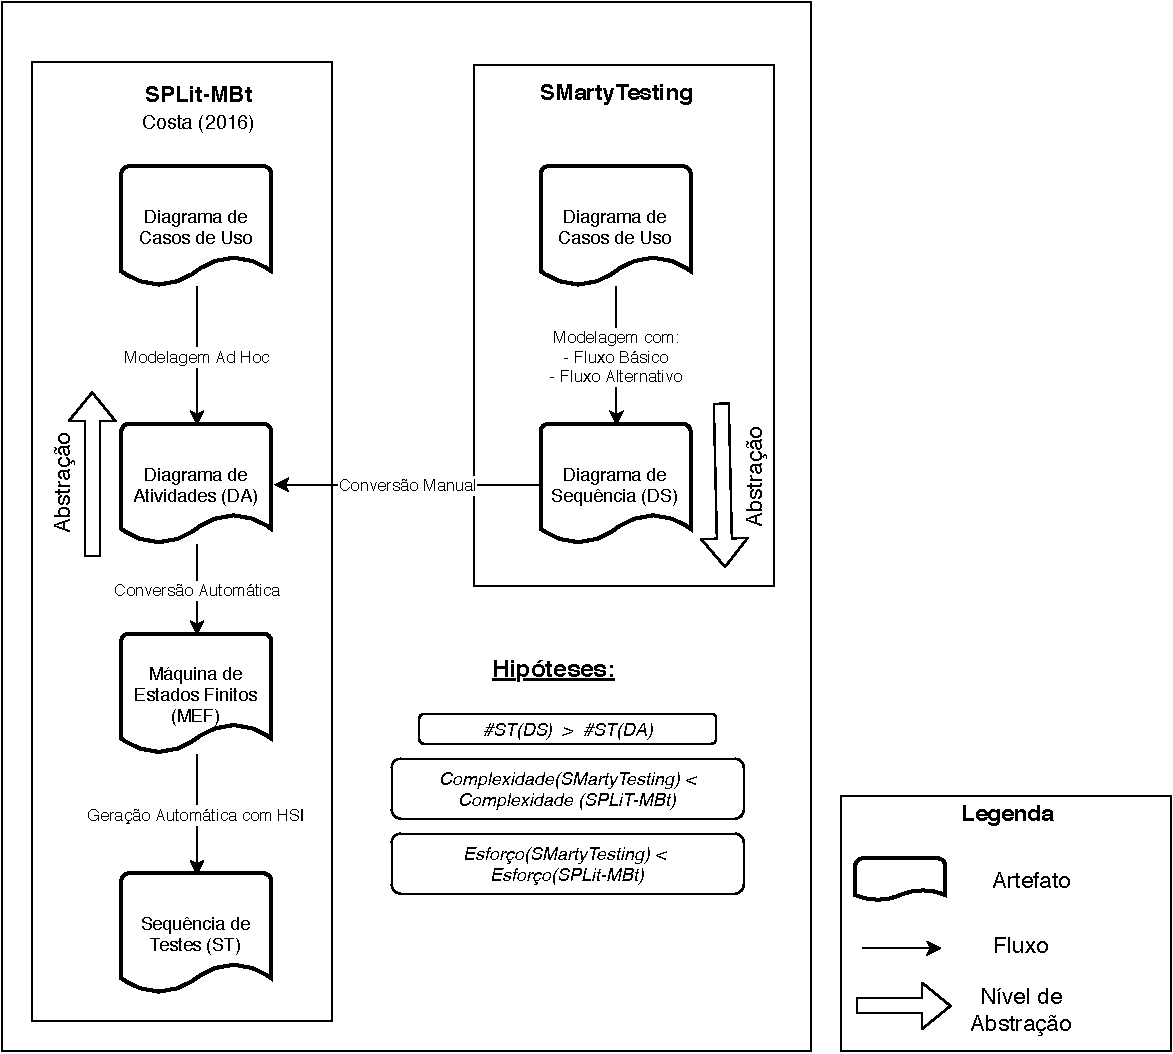
\includegraphics[width=0.85\textwidth]{hipoteses.pdf}
	\caption{Estudo de viabilidade e hipóteses definidas}
	\label{fig:hipoteses}
\end{figure}

\
\subsection{Instrumentação}
Para a geração das sequências de teste foram selecionados três diagramas que contivessem elementos necessários para a validação. A \ref{tab:diagramas_usados} contém as características assim como as variabilidades que cada diagrama possui.
\begin{table}[H]
	\centering
	\caption{Diagramas utilizados no processo de geração de sequências de teste.}
	\label{tab:diagramas_usados}
	\begin{tabular}{l|l|l}
		\hline
		\multicolumn{1}{c|}{\textbf{Modelos}} & \multicolumn{1}{c|}{\textbf{Característica}} & \multicolumn{1}{c}{\textbf{Variabilidade}} \\ \hline
		\begin{tabular}[c]{@{}l@{}}\textbf{\textit{Play Selected Game}}\\ \ref{fig:GamemenuCosta} (DA)\\ \ref{fig:GamemenuKleber} (DS)\end{tabular} & \begin{tabular}[c]{@{}l@{}}\textit{Play Selected Game} é a representação\\ do menu do jogo. Por meio dela é feita\\ a seleção de qual jogo será jogado.\end{tabular} & \begin{tabular}[c]{@{}l@{}}-ponto de variação\\ -variabilidade\\ \textit{-alternative\_OR}\end{tabular} \\ \hline
		\begin{tabular}[c]{@{}l@{}}\textbf{\textit{Save Game}}\\ \ref{fig:SaveGameCosta} (DA)\\ \ref{fig:SaveGameKleber} (DS)\end{tabular} & \textit{Save Game} é a ação de salvar o jogo. & \textit{-mandatory} \\ \hline
		\begin{tabular}[c]{@{}l@{}}\textbf{\textit{Pong Moves}}\\ \ref{fig:pongMovesCosta} (DA)\\ \ref{fig:pong_movesKleber1} (DS)\\\ref{fig:pong_movesKleber2} (DS)\end{tabular} & \begin{tabular}[c]{@{}l@{}}\textit{Pong Moves} são as ações e movimentos\\ do jogo \textit{Pong}.\end{tabular} & - não possui \\ \hline
	\end{tabular}
\end{table}

\subsection{Procedimentos de Análise}

O procedimento de análise segue conforme os critérios definidos na Seção \ref{cap4subsec:criterios}. Porém, para cada critério foi utilizada uma forma de análise diferente, como segue:
\begin{itemize}
	\item \textbf{CT.1:} utilizando comparação de resultados. Quantidade de casos de teste apresentados nas sequências de teste geradas por cada abordagem;
	\item \textbf{CT.2:} utilização de análise de quantidade de caminhos criados por cada geração de sequência. Se uma abordagem gera mais sequências, isso significa que mais caminhos podem ser visitados;
	\item \textbf{CT.3:} para o cálculo de complexidade, foi utilizada a complexidade ciclomática \ref{cap4subsec:ciclomatico}, métrica bastante utilizada para a determinação da quantidade de caminhos seguidos por uma aplicação computacional; e
	\item \textbf{CT.4:} esforço é baseado no tempo de utilização de cada abordagem, em que a abordagem que levar maior tempo para a construção do objetivo final é considerada a de maior esforço de utilização.
\end{itemize}


\section{Execução}
\label{cap4sec:execucaocomparativo}

\subsection{Geração de Sequências de Teste com SPLiT-MBt}
\label{cap4:subsubsec:diagrama_atividade}
Como mencionado anteriormente, foram utilizados três diagramas de atividades que fazem parte da LPS AGM e que foram modelados por \citet{costa2016split}, são eles: \ref{fig:GamemenuCosta}, \ref{fig:SaveGameCosta} e \ref{fig:pongMovesCosta}.

Neste trabalho, cada um deles é acompanhado de uma tabela contendo a sequência de teste gerada por SPLiT-MBt, são elas: \ref{tab:DAGamemenuCosta}, \ref{tab:DASaveGameCosta} e \ref{tab:DApongMovesCosta}. Esses dados serão utilizados na Seção \ref{cap4sec:analiseeinterpretacao} para comparação com diagramas equivalentes aos apresentados por \citet{costa2016split}. 
A \ref{fig:GamemenuCosta} apresenta um diagrama de atividades da LPS AGM que foi utilizado pela SPLiT-MBt para a comparação. 
\newpage
\begin{figure}[H]
	\centering
	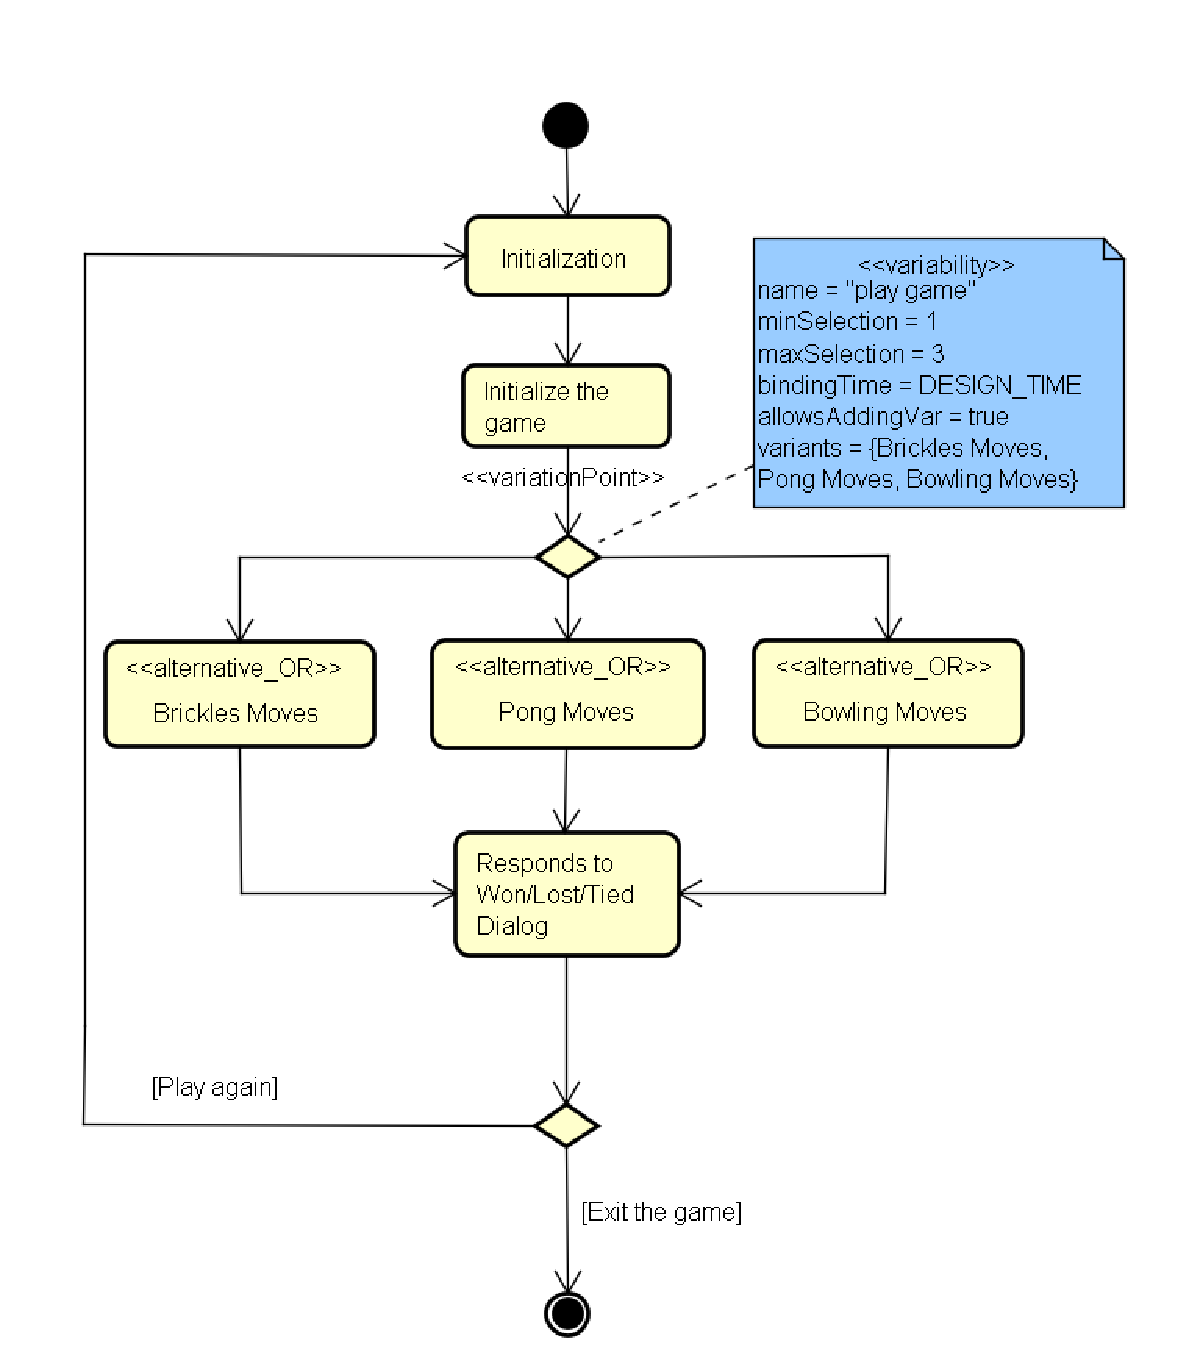
\includegraphics[width=0.75\textwidth]{1_Play_Selected_Game.pdf}
	\caption{Diagrama de Atividades \textit{Play Selected Game} \cite{costa2016split}}
	\label{fig:GamemenuCosta}
\end{figure}

A \ref{tab:DAGamemenuCosta} apresenta os resultados da sequência de teste gerada da \ref{fig:GamemenuCosta}.

%\begin{landscape}
	\begin{table}[H]
		\caption{Sequências de teste do DA \textit{Play Selected Game} da AGM da \ref{fig:GamemenuCosta} gerado por SPLiT-MBt}
		\label{tab:DAGamemenuCosta}
		\footnotesize
		\begin{tabular}{c|c|l|l}
			\hline
			\textbf{\begin{tabular}[c]{@{}c@{}}Sequência \\ de Teste\end{tabular}} & \textbf{Passo} & \textbf{Ação/Descrição} & \textbf{Resultado Esperado} \\ \hline
			\textit{Test Case} 1 & 1 & \begin{tabular}[c]{@{}l@{}}\textit{Initialization}\\ - \textit{Select Play from menu};\end{tabular} & \begin{tabular}[c]{@{}l@{}}Cria as instâncias padrão das\\ classes necessárias.\end{tabular} \\ \hline
			\textit{Test Case} 1 & 2 & \begin{tabular}[c]{@{}l@{}}\textit{Initialize the game}\\ - \textit{Left-click Button to begin play;}\end{tabular} & \begin{tabular}[c]{@{}l@{}}Inicie a ação do jogo e a animação\\começa.\end{tabular} \\ \hline
			\textit{Test Case} 1 & 3 & \begin{tabular}[c]{@{}l@{}}\textit{VP\_Initialize the game}\\ - \{;\\ - b\{\textit{alternative\_OR}\};\\ - c\{\textit{alternative\_OR}\};\\ - a\{\textit{alternative\_OR}\}\};\end{tabular} & \begin{tabular}[c]{@{}l@{}}\{.\\ As pás e o disco começam a se\\mover. \\ A bola começa a se mover. \\ Move a raquete horizontalmente\\para seguir a trilha do mouse \}.\end{tabular} \\ \hline
			\textit{Test Case} 1 & 4 & \begin{tabular}[c]{@{}l@{}}\textit{Responds to Won/Lost/Tied Dialog} \\ - \{;\\ - \textit{Responds to Won/Lost/Tied dialog};\\ - \textit{Responds to Won/Lost/Tied dialog};\\ - \textit{Responds to Won/Lost/Tied dialog} \};\end{tabular} & \begin{tabular}[c]{@{}l@{}}\{.\\ Retorne ao estado inicial do\\ tabuleiro. \\Retorne ao estado inicial do\\tabuleiro. \\A caixa de diálogo para reproduzir\\ novamente é apresentada\}.\end{tabular} \\ \hline
			\textit{Test Case} 1 & 5 & \begin{tabular}[c]{@{}l@{}}\textit{Initialization}\\ - \textit{Respond``yes" in the dialog to play again};\end{tabular} & \begin{tabular}[c]{@{}l@{}}Retorna o tabuleiro de jogo ao seu\\ estado inicializado, pronto para jogar.\end{tabular} \\ \hline
		\end{tabular}
	\end{table}
%\end{landscape}

A \ref{fig:SaveGameCosta} apresenta um diagrama de atividades da LPS AGM que foi utilizado pela SPLiT-MBt para a comparação. 

\begin{figure}[H]
	\centering
	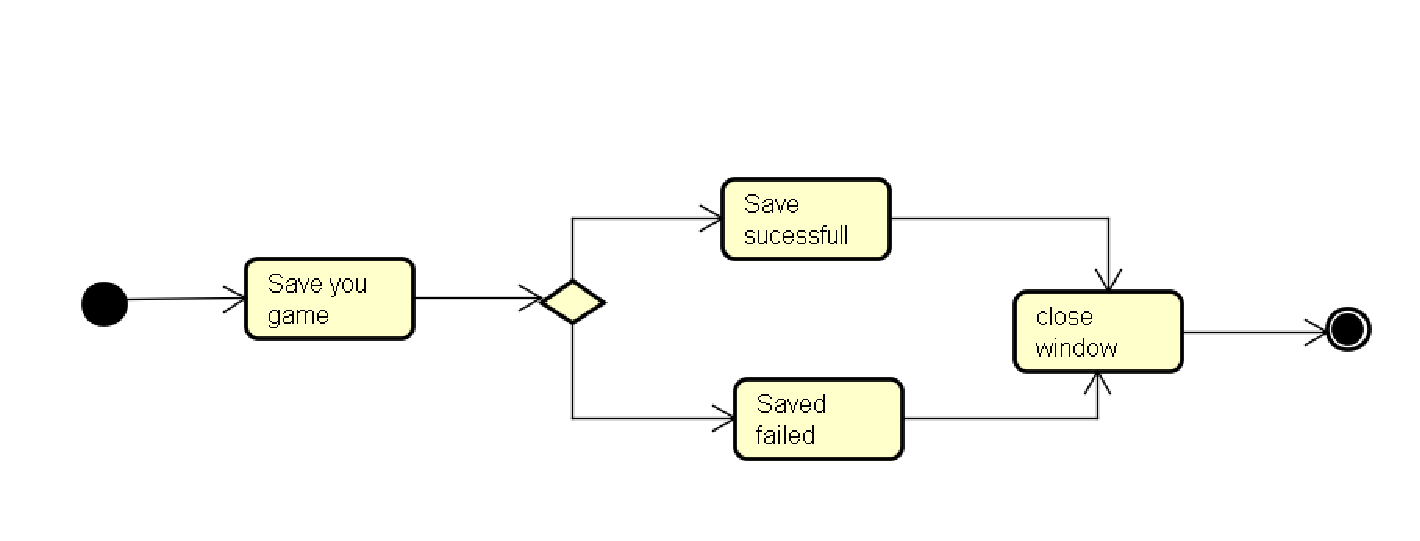
\includegraphics[width=\textwidth]{2_Save_Game.pdf}
	\caption{Diagrama de Atividades \textit{Save Game} \cite{costa2016split}}
	\label{fig:SaveGameCosta}
\end{figure}
\newpage
A \ref{tab:DASaveGameCosta} apresenta os resultados da sequência de teste gerada da \ref{fig:SaveGameCosta}.

	\begin{table}[H]
		\caption{Sequências de teste do DA \textit{Save Game} da \ref{fig:SaveGameCosta} geradas por SPLiT-MBt}
		\label{tab:DASaveGameCosta}
		\begin{tabular}{p{2.5cm}|p{1cm}|p{6cm}|p{5cm}}
			\hline
			\textbf{\begin{tabular}[c]{@{}c@{}}Sequência \\ de Teste\end{tabular}} & \textbf{Passo} & \textbf{Ação/Descrição} & \textbf{Resultado Esperado} \\ \hline
			\textit{Test Case} 1 & 1 & \begin{tabular}[c]{@{}l@{}}\textit{Save your game}\\ - \textit{save GAME window are showed};\end{tabular} & Termine o jogo. \\ \hline
			\textit{Test Case} 1 & 2 & \begin{tabular}[c]{@{}l@{}}\textit{Saved failed}\\ - \textit{click SAVE GAME  button};\end{tabular} & mensagem SALVAR JOGO com falha é mostrada. \\ \hline
			\textit{Test Case} 1 & 3 & \begin{tabular}[c]{@{}l@{}}\textit{close window}\\ - \textit{Click close SAVE THE GAME};\end{tabular} & A janela SALVAR JOGO é fechada. \\ \hline
			\textit{Test Case} 2 & 1 & \begin{tabular}[c]{@{}l@{}}\textit{Save your game}\\ - \textit{save GAME window are showed};\end{tabular} & Termine o jogo. \\ \hline
			\textit{Test Case} 2 & 2 & \begin{tabular}[c]{@{}l@{}}\textit{Save sucessfull}\\ - \textit{click SAVE GAME button};\end{tabular} & messagem SALVAR JOGO é mostrada. \\ \hline
			\textit{Test Case} 2 & 3 & \begin{tabular}[c]{@{}l@{}}\textit{close window}\\ - \textit{click close SAVE GAME button};\end{tabular} & A janela SALVAR JOGO é fechada. \\ \hline
		\end{tabular}
	\end{table}

A \ref{fig:pongMovesCosta} apresenta um diagrama de atividades da LPS AGM que foi utilizado pela SPLiT-MBt para a comparação.

\begin{figure}[H]
	\centering
	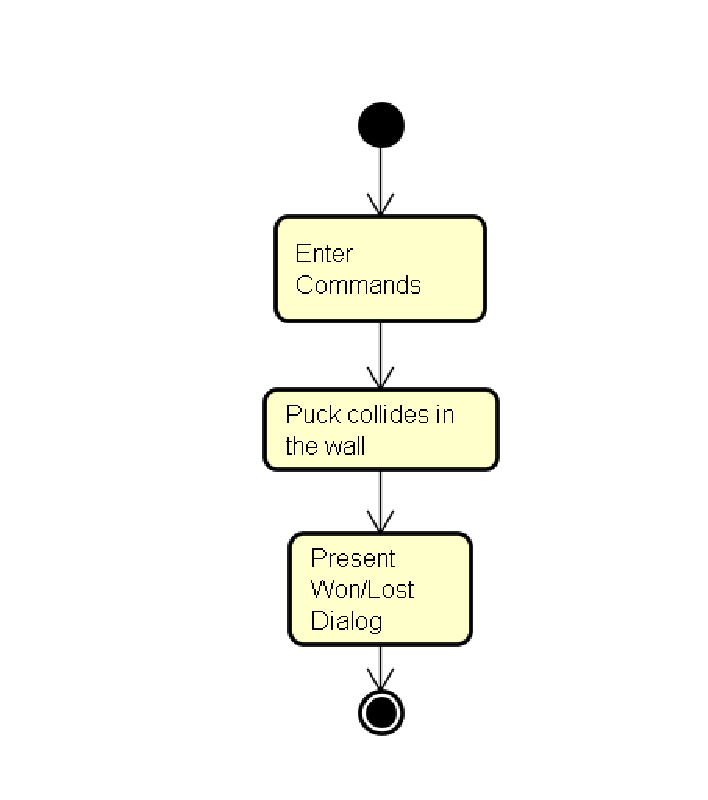
\includegraphics[width=0.2\textwidth]{3_pong_Moves.pdf}
	\caption{Diagrama de Atividades \textit{Pong Moves} \cite{costa2016split}}
	\label{fig:pongMovesCosta}
\end{figure}
\newpage
A \ref{tab:DApongMovesCosta} apresenta os resultados da sequência de teste gerada da \ref{fig:pongMovesCosta}.

	\begin{table}[H]
		\caption{Sequencia de teste do DA \textit{Pong Moves} da \ref{fig:pongMovesCosta} gerada por SPLiT-MBt}
		\label{tab:DApongMovesCosta}
		\begin{tabular}{p{2.5cm}|p{1cm}|p{5.5cm}|p{6cm}}
			\hline
			\textbf{\begin{tabular}[c]{@{}c@{}}Sequência \\ de Teste\end{tabular}} & \textbf{Passo} & \textbf{Ação/Descrição} & \textbf{Resultado Esperado} \\ \hline
			\textit{Test Case} 1 & 1 & \begin{tabular}[c]{@{}l@{}}\textit{Enter Commands}\\ - \textit{Pong};\end{tabular} & Disco começa a se mover. \\ \hline
			\textit{Test Case} 1 & 2 & \begin{tabular}[c]{@{}l@{}}\textit{Puck collides in the wall}\\ - \textit{Let the puck collide into} \\ \textit{the walls};\end{tabular} & \begin{tabular}[c]{@{}l@{}}Com base nas regras, o disco é \\ absorvido ou muda de direção \\ de acordo com as leis da física.\end{tabular} \\ \hline
			\textit{Test Case} 1 & 3 & \begin{tabular}[c]{@{}l@{}}\textit{Present Won/Lost Dialog} \\ - \textit{The puck is absorbed by the} \\ \textit{left or right side of the playing} \\ \textit{field};\end{tabular} & A caixa de diálogo Ganhos / Perdas é apresentada. \\ \hline
		\end{tabular}
	\end{table}

\newpage

\subsection{Geração de Sequências de Teste com \textit{SMartyTesting}}
\label{cap4subsubsec:diagrama_sequencia}

Após a geração da sequência de teste com DA como artefatos de entrada da SPLiT-MBt, são utilizados DS criados por \citet{marcolino2017variability}, equivalentes aos DA criados por \citet{costa2016split} que são os da \ref{fig:GamemenuKleber}, \ref{fig:SaveGameKleber} e \ref{fig:pong_movesKleber1}.


Essa equivalência se deve ao fato do nível de abstração utilizado, um exemplo é a \ref{fig:SaveGameCosta} que representa o \textit{Save Game}, nela são observadas duas condições, onde houve sucesso e onde houve falha no salvamento. Nesse caso, a representação em DS por ser mais próxima ao código dar-se-ia em dois diagramas: um para sucesso e outro para falha. A \ref{fig:SaveGameKleber} representa somente a condição de sucesso.   

Após essa criação, os DS foram utilizados em \textit{SMartyTesting} para a geração de sequências de teste para comparação. Na etapa inicial foi realizada a conversão para DA conforme pode ser visto nas figuras: \ref{fig:GamemenuKleberDStoDA}, \ref{fig:SaveGameKleberDStoDA} e \ref{fig:pong_movesDS_to_DA1}, que na etapa seguinte foram utilizados para a geração das sequências de teste: \ref{tab:GamemenuKleberDStoDA}, \ref{tab:SaveGameKleberDStoDA} e \ref{tab:pong_movesDS_to_DA}.

A \ref{fig:GamemenuKleber} apresenta um diagrama de sequência da LPS AGM que foi utilizado por \textit{SMartyTesting} para a conversão para DA.

%\begin{landscape}
	\begin{figure}[H]
		\centering
		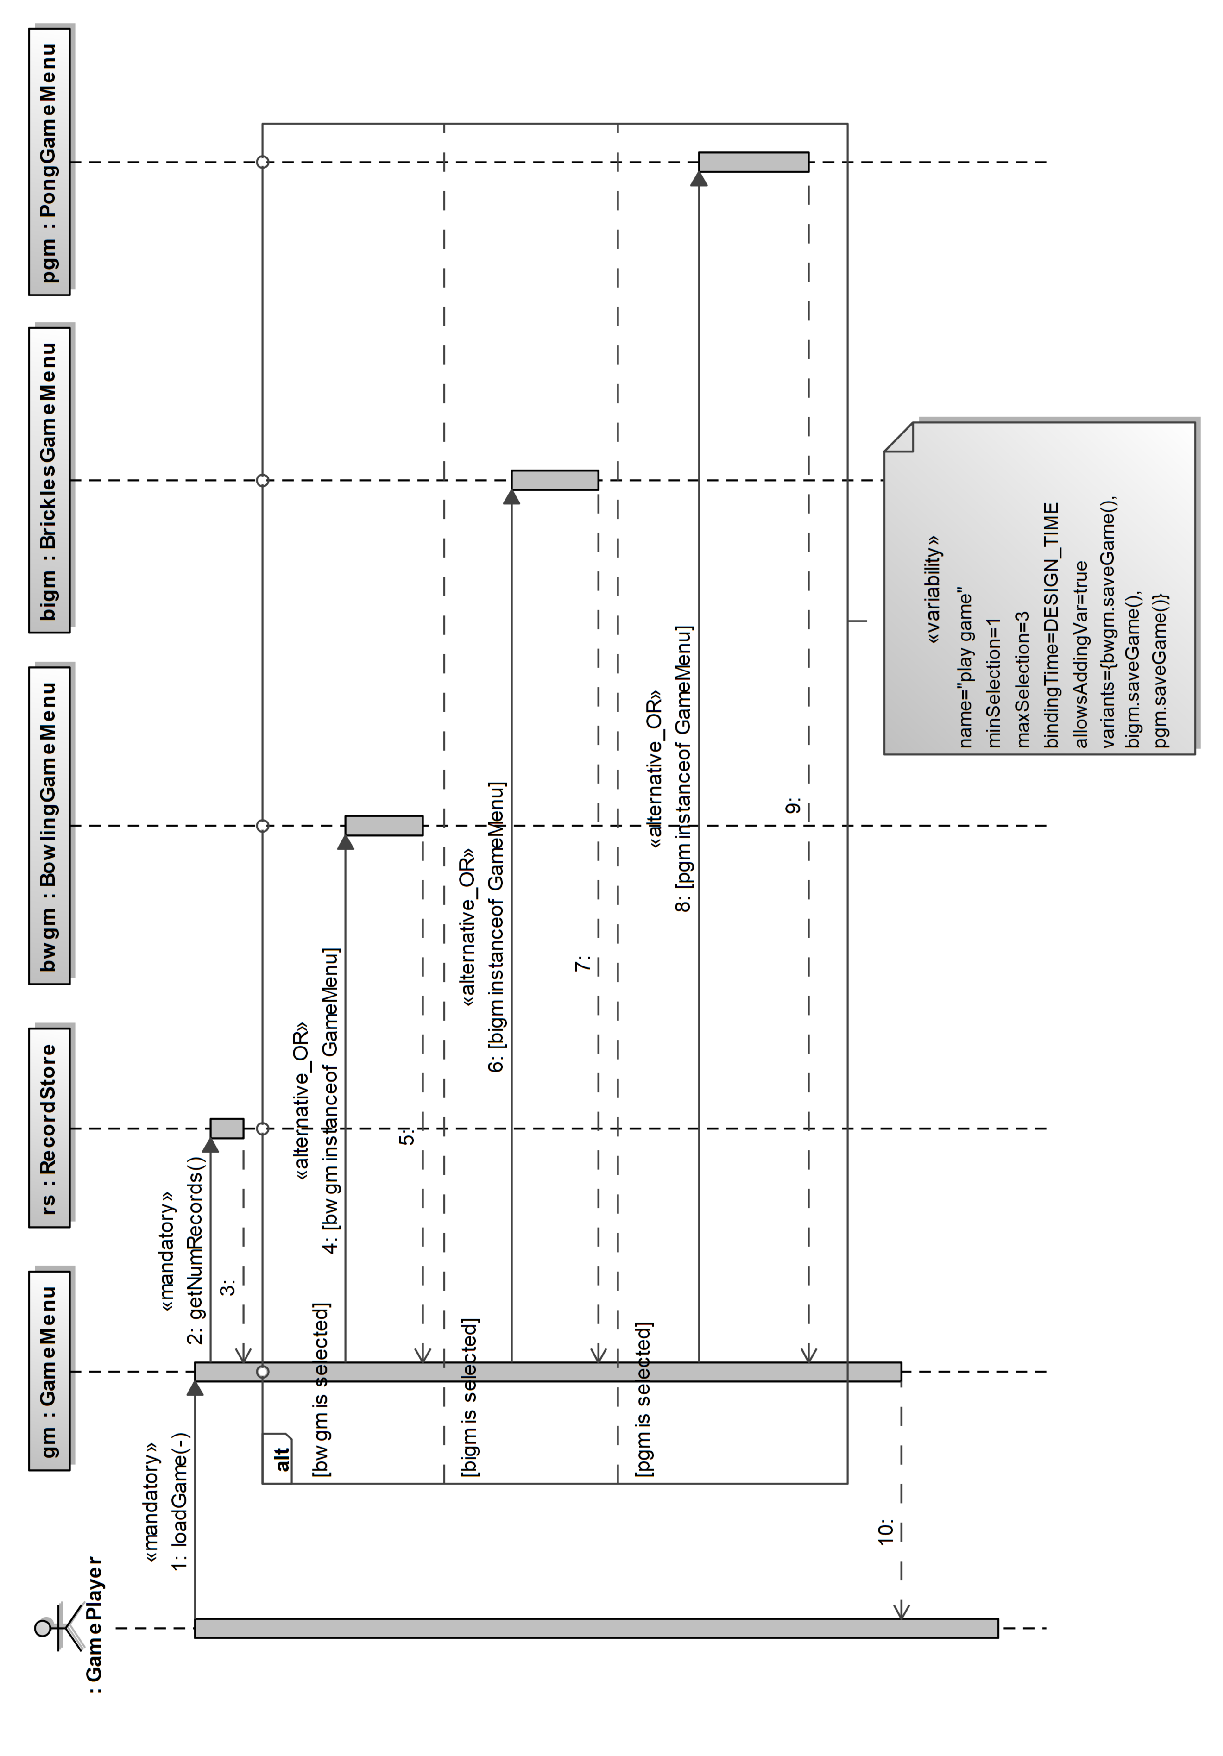
\includegraphics[width=0.75\textwidth]{1_loadGame_LP_View2.pdf}
		\caption{Diagrama de Sequência \textit{Play Selected Game} \cite{marcolino2017variability}}
		\label{fig:GamemenuKleber}
	\end{figure}
%\end{landscape}

A \ref{fig:GamemenuKleberDStoDA} apresenta um diagrama de atividades da LPS AGM que foi convertido por \textit{SMartyTesting} para a geração de sequências de teste.

%\begin{landscape}
	\begin{figure}[H]
		\centering
		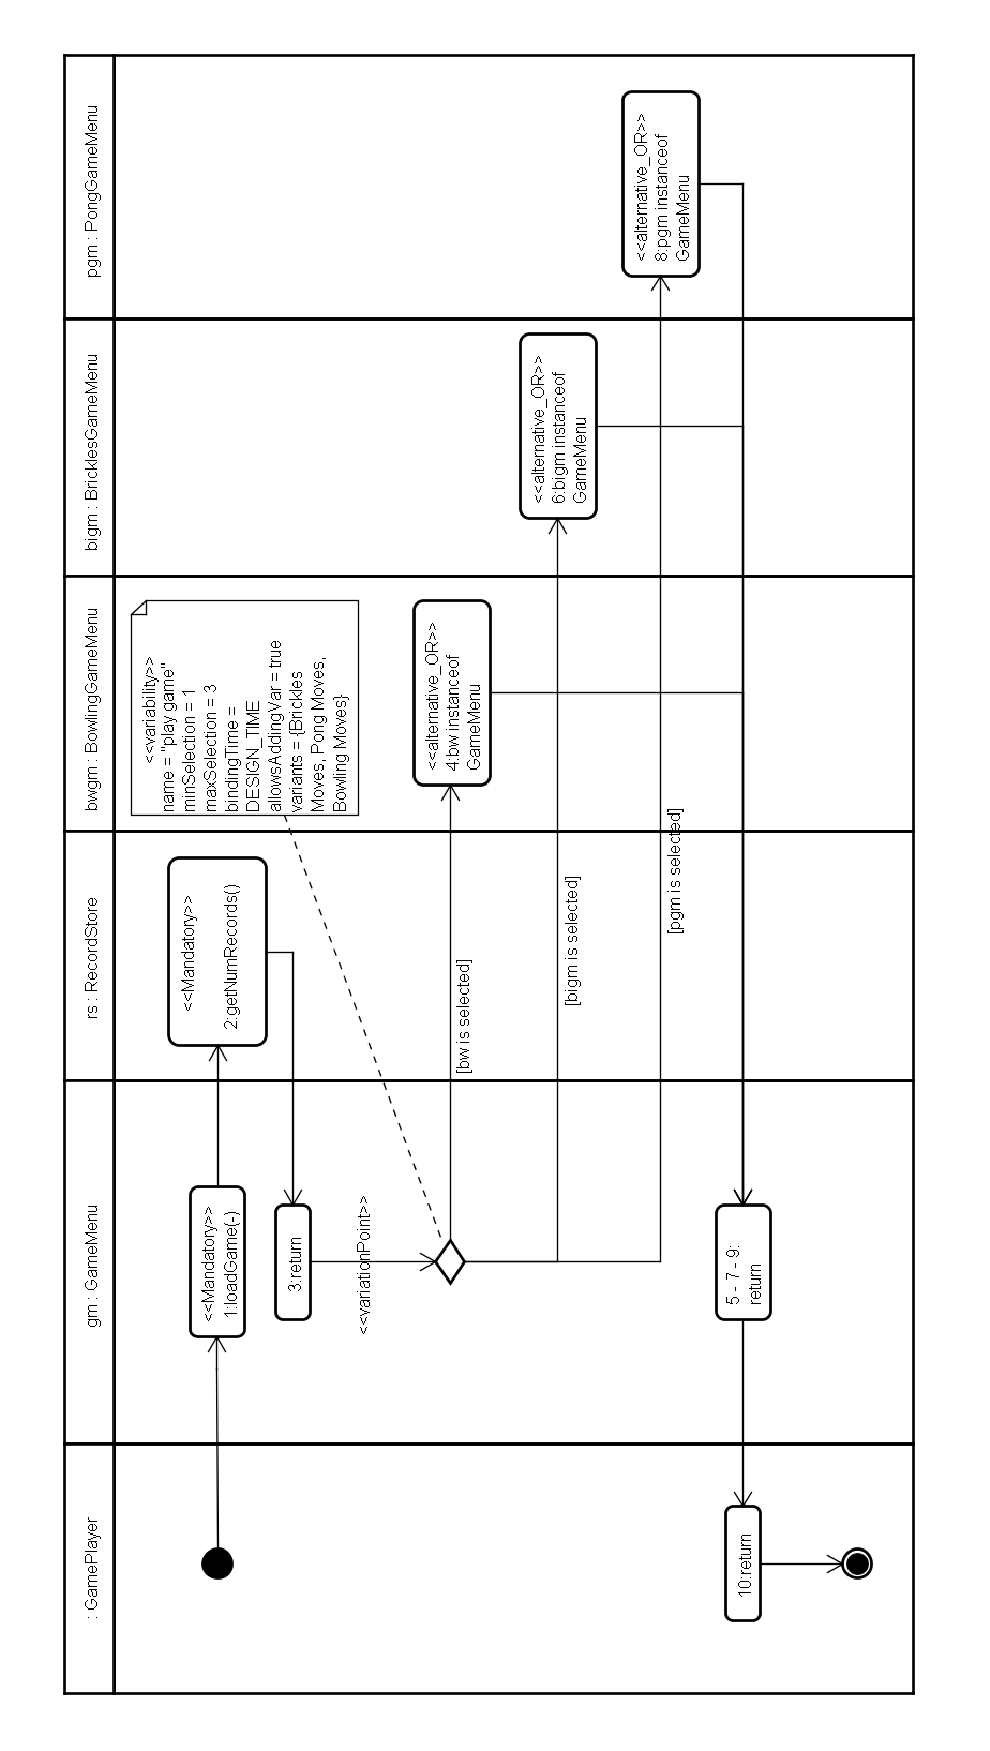
\includegraphics[width=0.63\textwidth]{1_Play_Selected_Game_DS_to_DA2.pdf}
		\caption{Diagrama de Atividades resultantes do Diagrama de Sequência da \ref{fig:GamemenuKleber}}
		\label{fig:GamemenuKleberDStoDA}
	\end{figure}
%\end{landscape}

A \ref{tab:GamemenuKleberDStoDA} apresenta os resultados da sequência de teste gerada da \ref{fig:GamemenuKleberDStoDA}.

%\begin{landscape}
	\begin{table}[H]
		\caption{Sequências de casos de teste DA da \ref{fig:GamemenuKleberDStoDA} geradas por \textit{SMartyTesting}}
		\label{tab:GamemenuKleberDStoDA}
		\footnotesize
		\begin{tabular}{c|c|l|l}
			\hline
			\textbf{\begin{tabular}[c]{@{}c@{}}Sequência \\ de Teste\end{tabular}} & \textbf{Passo} & \textbf{Ação/Descrição} & \textbf{Resultado Esperado} \\ \hline
			\textit{Test Case} 1 & 1 & \begin{tabular}[c]{@{}l@{}}1:\textit{loadGame}(-)\\ - \textit{Game Player} dispara método \\ \textit{loadGame}\{\textit{Mandatory}\};\end{tabular} & \textit{loadGame} é carregado. \\ \hline
			\textit{Test Case} 1 & 2 & \begin{tabular}[c]{@{}l@{}}2:\textit{getNumRecords}()\\ - \textit{Game menu} após carregado faz \\ uso do método \textit{getNumRecords}\{\textit{Mandatory}\};\end{tabular} & acessa dados de \textit{recordStore}. \\ \hline
			\textit{Test Case} 1 & 3 & \begin{tabular}[c]{@{}l@{}}3:\textit{return}\\ - \textit{recordStore} envia mensagens de retorno;\end{tabular} & \begin{tabular}[c]{@{}l@{}}Dados de pontuação são\\ retornados por\\ \textit{getNumrecords} para \textit{GameMenu}.\end{tabular} \\ \hline
			\textit{Test Case} 1 & 4 & \begin{tabular}[c]{@{}l@{}}VP\_3:\textit{return}\\ - \{;\\ - Opção bw é selecionada\{\textit{alternative\_OR\}};\\ - Opção bigm é selecionada\{\textit{alternative\_OR\}};\\ - Opção pgm é selecionada\{\textit{alternative\_OR\}}\};\end{tabular} & \begin{tabular}[c]{@{}l@{}}\{.\\ Instancia recurso da opção\\ \textit{bowling}.\\ instancia recurso da opção\\ bigm \textit{brickles}.\\ instancia recurso da opção\\ \textit{pong}\}.\end{tabular} \\ \hline
			\textit{Test Case} 1 & 5 & \begin{tabular}[c]{@{}l@{}}5 - 7 - 9:\textit{return}\\ - \{;\\ - Retorno da opção bw;\\ - Retorno da opção bigm;\\ - Retorno da opção pgm\};\end{tabular} & \begin{tabular}[c]{@{}l@{}}\{.\\ Retorna após bw \textit{instanceof}\\ \textit{GameMenu} for executada.\\ Retorna após bigm \textit{instanceof}\\ GameMenu for executada.\\ Retorna após pgm \textit{instanceof}\\ \textit{GameMenu} for executada\}.\end{tabular} \\ \hline
			\textit{Test Case} 1 & 6 & \begin{tabular}[c]{@{}l@{}}10:\textit{return}\\ - Retorno da informação ao \textit{Game Player};\end{tabular} & \begin{tabular}[c]{@{}l@{}}\textit{Player} recebe retorno da ação\\ escolhida.\end{tabular} \\ \hline
		\end{tabular}
	\end{table}
%\end{landscape}

A \ref{fig:SaveGameKleber} apresenta um diagrama de sequência da LPS AGM que foi utilizado por \textit{SMartyTesting} para a conversão para DA.

\begin{landscape}
	\begin{figure}[H]
		\centering
		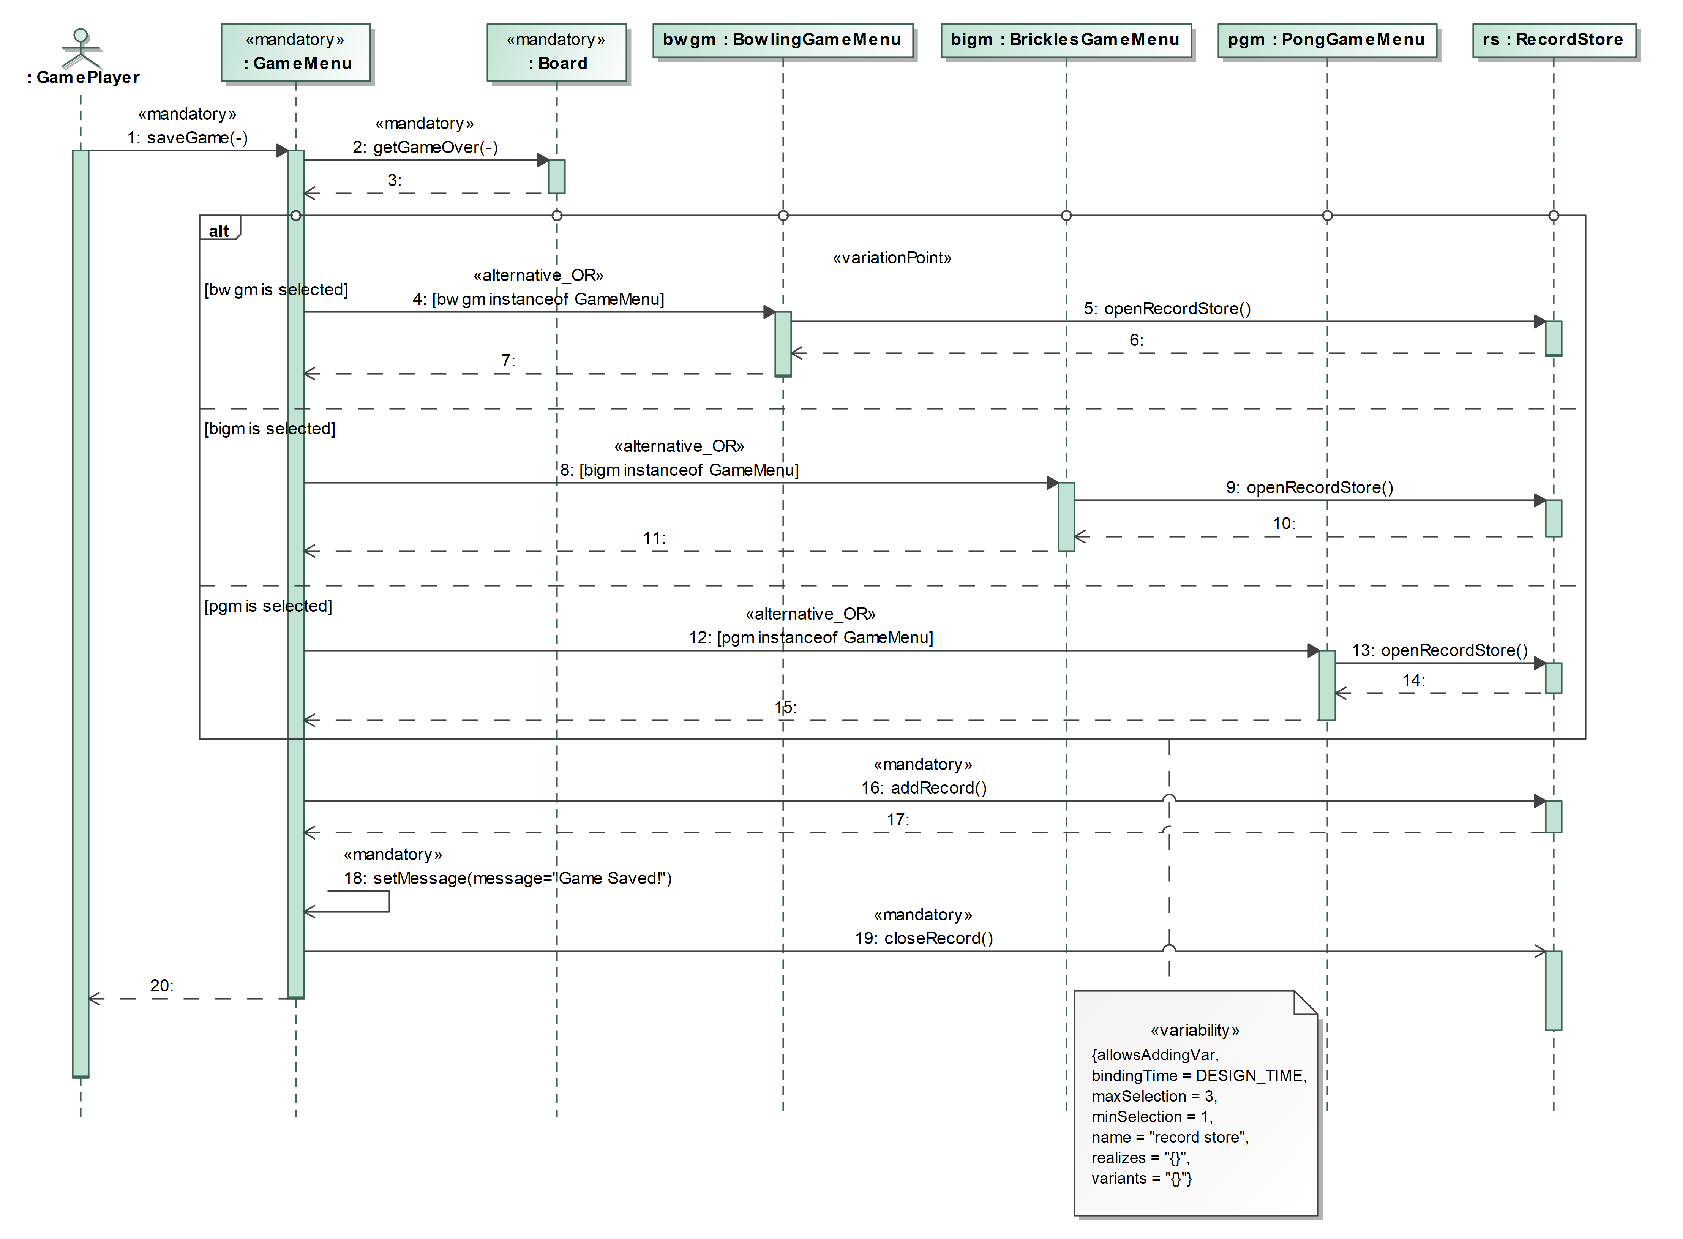
\includegraphics[scale=0.70]{2_saveGame_LP_View.pdf}
		\caption{Diagrama de Sequência \textit{Save Game} \cite{marcolino2017variability}}
		\label{fig:SaveGameKleber}
	\end{figure}
\end{landscape}

A \ref{fig:SaveGameKleberDStoDA} apresenta um diagrama de atividades da LPS AGM que foi convertido por \textit{SMartyTesting} para a geração de sequências de teste.

%\begin{landscape}
	\begin{figure}[H]
		\centering
		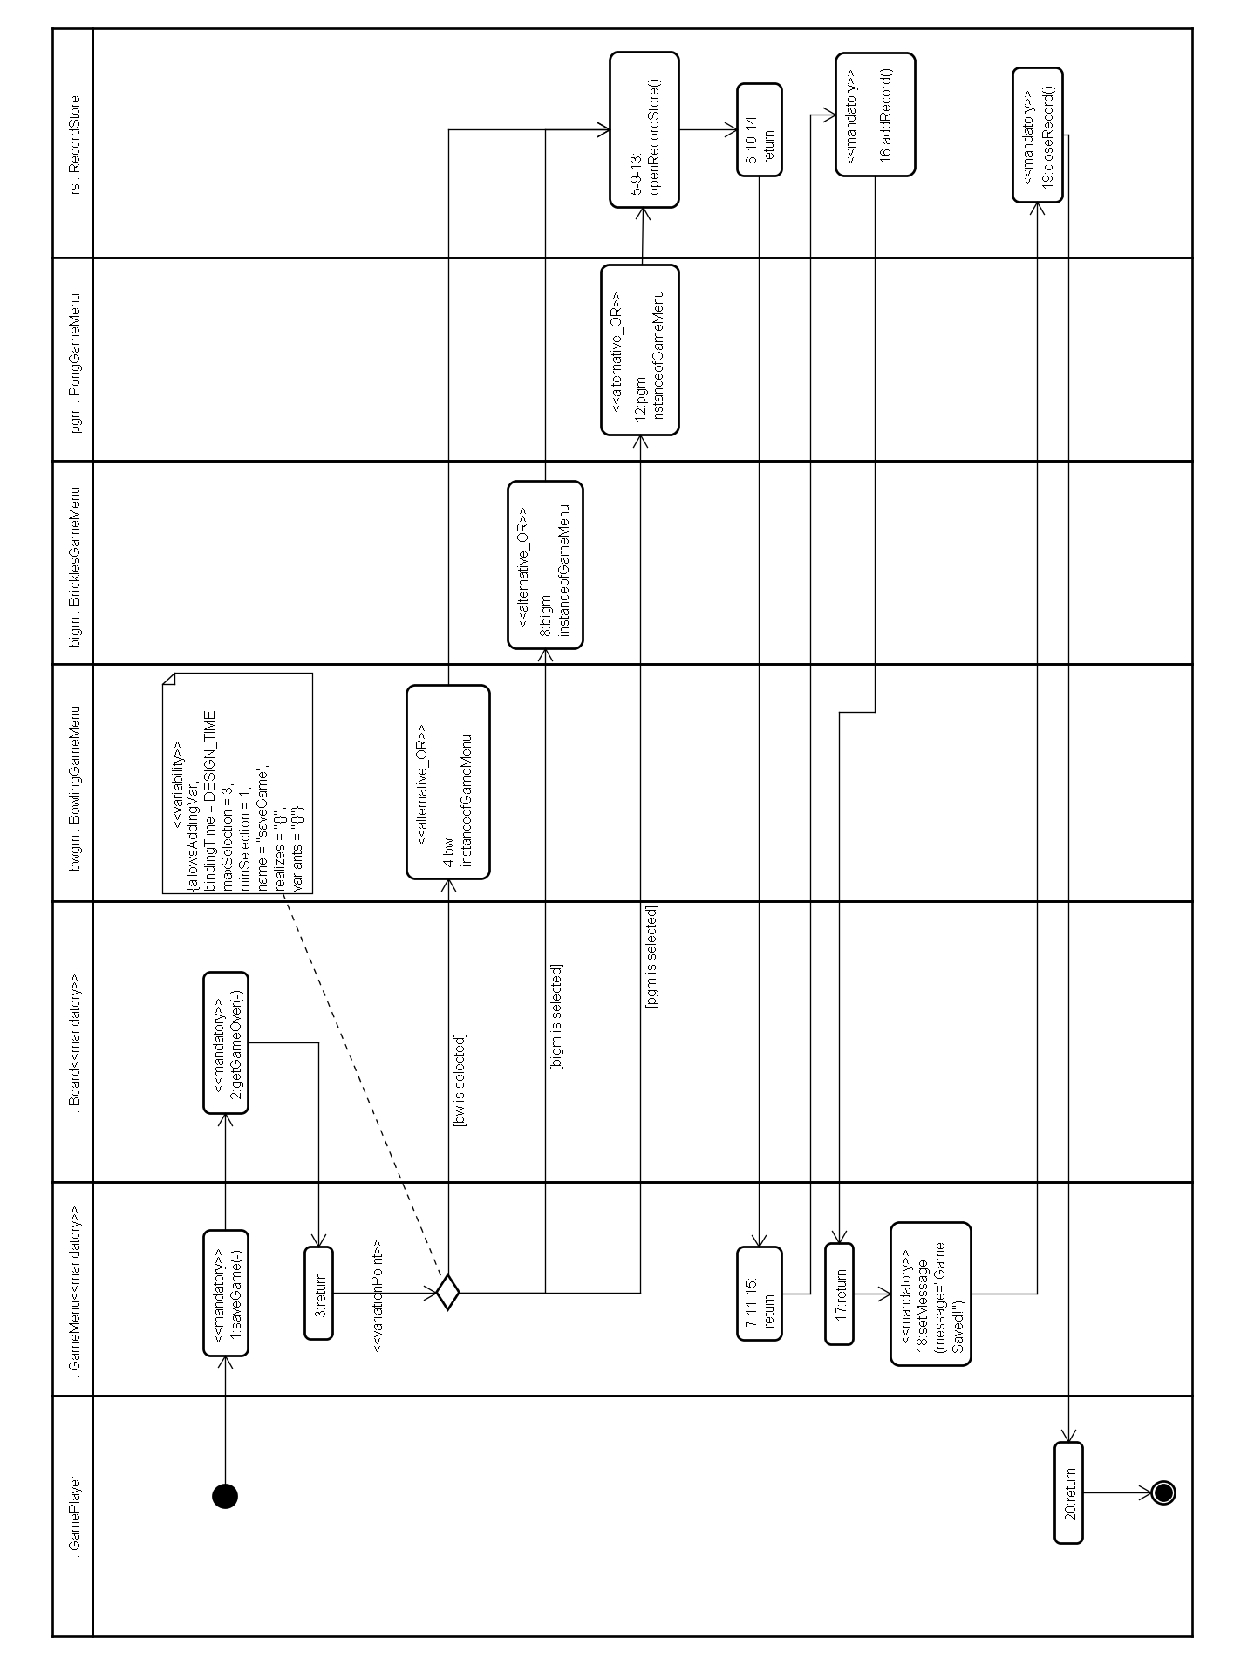
\includegraphics[width=0.8\textwidth]{2_saveGame_LP_View_DS_to_DA2.pdf}
		\caption{Diagrama de Atividades resultante dos Diagrama de Sequência da \ref{fig:SaveGameKleber}}
		\label{fig:SaveGameKleberDStoDA}
	\end{figure}
%\end{landscape}

A \ref{tab:SaveGameKleberDStoDA} apresenta os resultados da sequência de teste gerada da \ref{fig:SaveGameKleberDStoDA}.

\begin{landscape}
	\begin{table}[h!]
		\caption{Sequências de teste DA da \ref{fig:SaveGameKleberDStoDA} geradas por \textit{SMartyTesting}}
		\label{tab:SaveGameKleberDStoDA}
		\begin{tabular}{c|c|l|l}
			\hline
			\textbf{\begin{tabular}[c]{@{}c@{}}Sequência \\ de Teste\end{tabular}} & \textbf{Passo} & \textbf{Ação/Descrição} & \textbf{Resultado Esperado} \\ \hline
			\textit{Test Case} 1 & 1 & \begin{tabular}[c]{@{}l@{}}1:\textit{saveGame}(-)\\ - \textit{GamePlayer} dispara método \\ \textit{saveGame}\{\textit{mandatory}\};\end{tabular} & \textit{GameMenu} é carregado. \\ \hline
			\textit{Test Case} 1 & 2 & \begin{tabular}[c]{@{}l@{}}2:\textit{getGameOver}(-)\\ - \textit{GameMenu} dispara método \\ \textit{getGameOver}\{\textit{mandatory}\};\end{tabular} & \textit{Board} verifica ação. \\ \hline
			\textit{Test Case} 1 & 3 & \begin{tabular}[c]{@{}l@{}}3:\textit{return}\\ - \textit{Board} retorna solicitação;\end{tabular} & Valor retorna para jogo selecionado. \\ \hline
			\textit{Test Case} 1 & 4 & \begin{tabular}[c]{@{}l@{}}VP\_3:\textit{return}\\ - \{; bw é selecionado\{\textit{alternative\_OR}\};\\ - bigm é selecionado\{\textit{alternative\_OR}\};\\ - pgm é selecionado\{\textit{alternative\_OR}\}\};\end{tabular} & \begin{tabular}[c]{@{}l@{}}\{.\\ dispara método \textit{instanceofGameMenu}.\\ dispara método \textit{instanceofGameMenu}.\\ dispara método \textit{instanceofGameMenu}\}.\end{tabular} \\ \hline
			\textit{Test Case} 1 & 5 & \begin{tabular}[c]{@{}l@{}}5-9-13:\textit{openRecordStore}()\\ - \{; bw envia dados para método \textit{openRecordStore};\\ - bigm envia dados para método \textit{openRecordStore};\\ - pgm envia dados para método \textit{openRecordStore}\};\end{tabular} & \begin{tabular}[c]{@{}l@{}}\{.\\ dados são utilizados por \textit{openRecordStore}.\\ dados são utilizados por \textit{openRecordStore}.\\ dados são utilizados por \textit{openRecordStore}\}.\end{tabular} \\ \hline
			\textit{Test Case} 1 & 6 & \begin{tabular}[c]{@{}l@{}}6-10-14:\textit{return}\\ - \textit{operRecordStore} retorna para bw - bigm - pgm;\end{tabular} & confirma se possui dados disponíveis. \\ \hline
			\textit{Test Case} 1 & 7 & \begin{tabular}[c]{@{}l@{}}7-11-15:\textit{return}\\ - Return dos dados para \textit{GameMenu};\end{tabular} & \begin{tabular}[c]{@{}l@{}}dados disponíveis são retornados \\ para serem adicionados.\end{tabular} \\ \hline
			\textit{Test Case} 1 & 8 & \begin{tabular}[c]{@{}l@{}}16:\textit{addRecord}()\\ - acionado método \textit{addRecord}\{\textit{mandatory}\};\end{tabular} & Dados são salvos. \\ \hline
			\textit{Test Case} 1 & 9 & \begin{tabular}[c]{@{}l@{}}17:\textit{return}\\ - retorna ação do \textit{addRecord};\end{tabular} & Confirma persistência dos dados. \\ \hline
			\textit{Test Case} 1 & 10 & \begin{tabular}[c]{@{}l@{}}18:\textit{setMessage(message="Game Saved!")}\\ - dispara mensagem de confirmação\{\textit{mandatory}\};\end{tabular} & Mensagem de confirmação apresentada. \\ \hline
			\textit{Test Case} 1 & 11 & \begin{tabular}[c]{@{}l@{}}19:\textit{closeRecord}()\\ - Dispara método \textit{closeRecord}\{\textit{mandatory}\};\end{tabular} & Método encerra operação. \\ \hline
			\textit{Test Case} 1 & 12 & \begin{tabular}[c]{@{}l@{}}20:\textit{return}\\ - retornar confirmação da operação;\end{tabular} & \begin{tabular}[c]{@{}l@{}}Concluída com sucesso devolver \\ Confirmação ao usuário\end{tabular} \\ \hline
		\end{tabular}
	\end{table}
\end{landscape}

A \ref{fig:pong_movesKleber1} e a \ref{fig:pong_movesKleber2} apresentam um diagrama de sequência da LPS AGM que foi utilizado por \textit{SMartyTesting} para a conversão para DA.

%\begin{landscape}
	\begin{figure}[H]
		\centering
		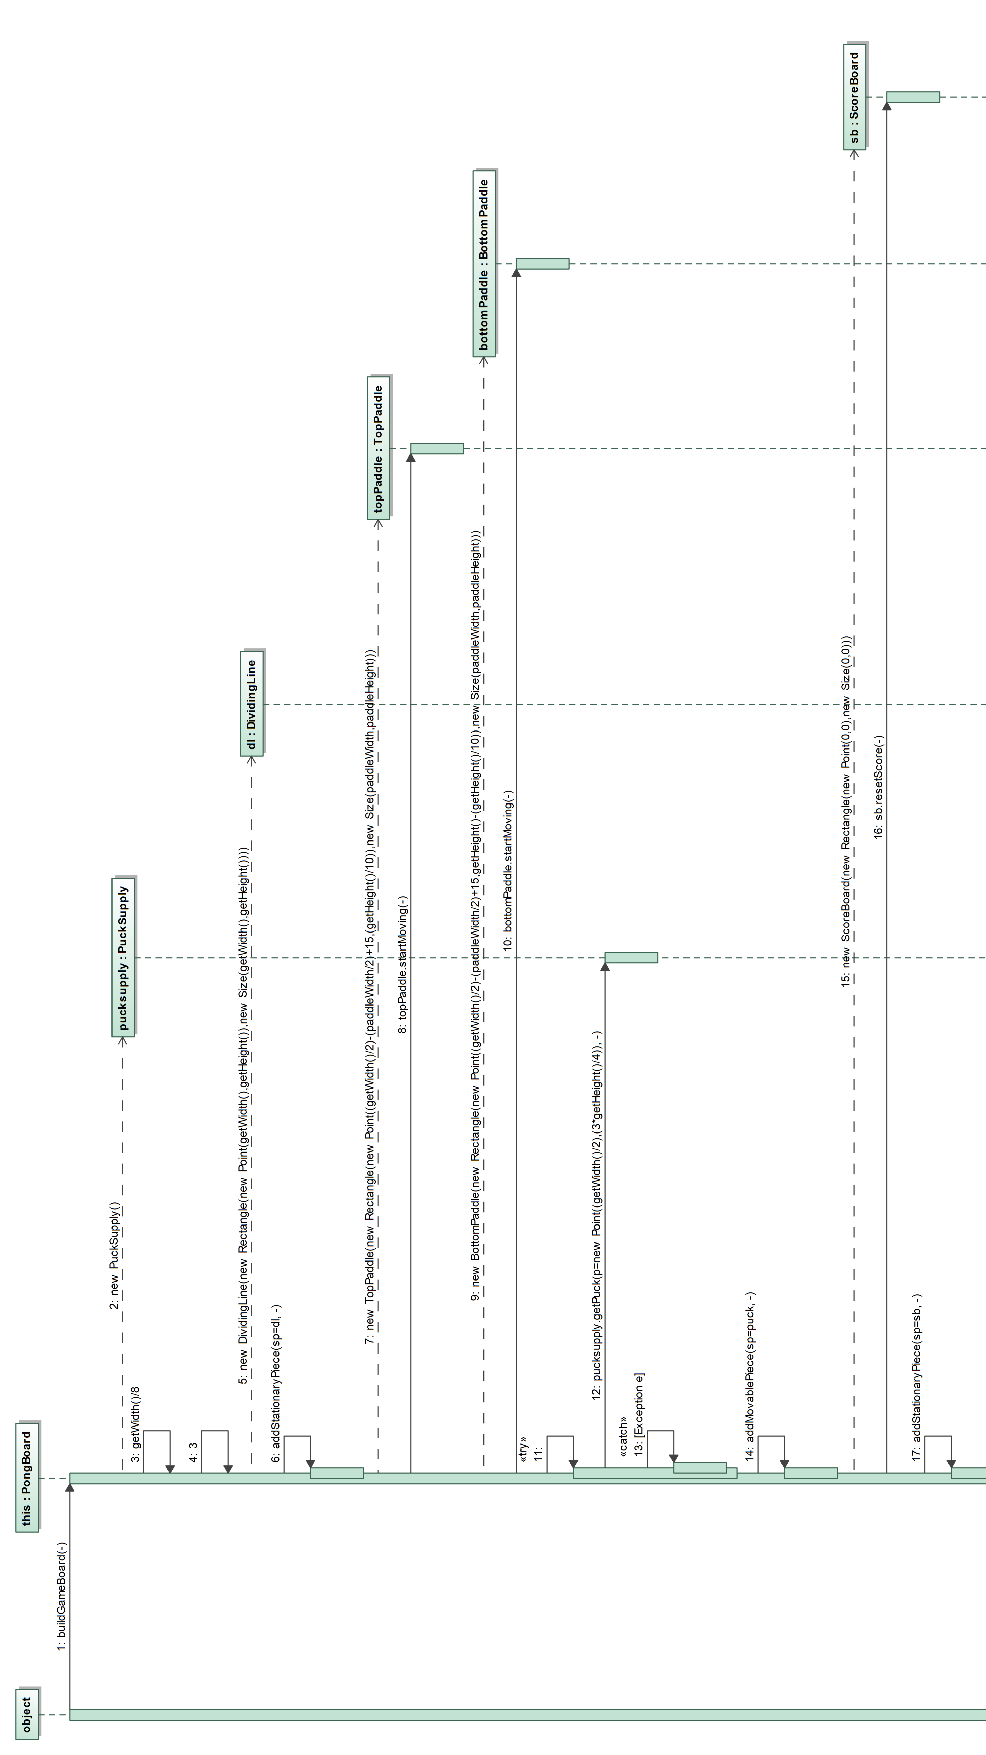
\includegraphics[width=0.7\textwidth]{3_DS_pong_moves_1_2.pdf}
		\caption{Diagrama de Sequência \textit{Pong Moves} 1 \cite{marcolino2017variability}}
		\label{fig:pong_movesKleber1}
	\end{figure}
%\end{landscape}

\begin{landscape}
	\begin{figure}[H]
		\centering
		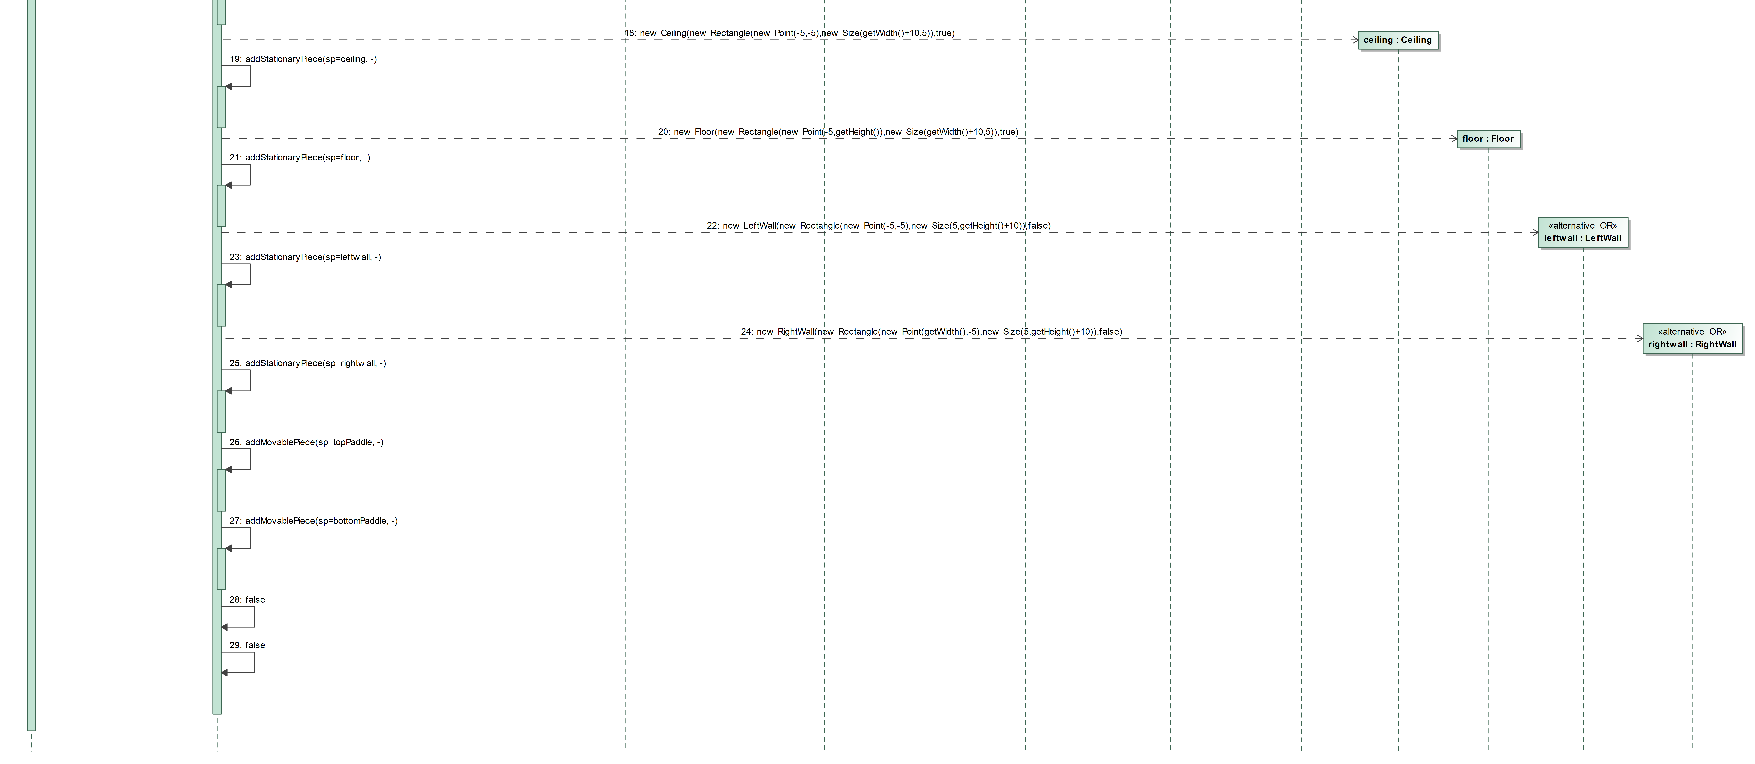
\includegraphics[scale=0.75]{3_DS_pong_moves_2.pdf}
		\caption{Diagramas de Sequência \textit{Pong Moves} 2 \cite{marcolino2017variability}}
		\label{fig:pong_movesKleber2}
	\end{figure}
\end{landscape}

As \ref{fig:pong_movesDS_to_DA1} e \ref{fig:pong_movesDS_to_DA2} apresentam um diagrama de atividades da LPS AGM que foi convertido por \textit{SMartyTesting} para a geração de sequências de teste.

A \ref{tab:pong_movesDS_to_DA} apresenta os resultados da sequência de teste gerada das \ref{fig:pong_movesDS_to_DA1} e \ref{fig:pong_movesDS_to_DA2}

%\begin{landscape}
	\begin{figure}[H]
		\centering
		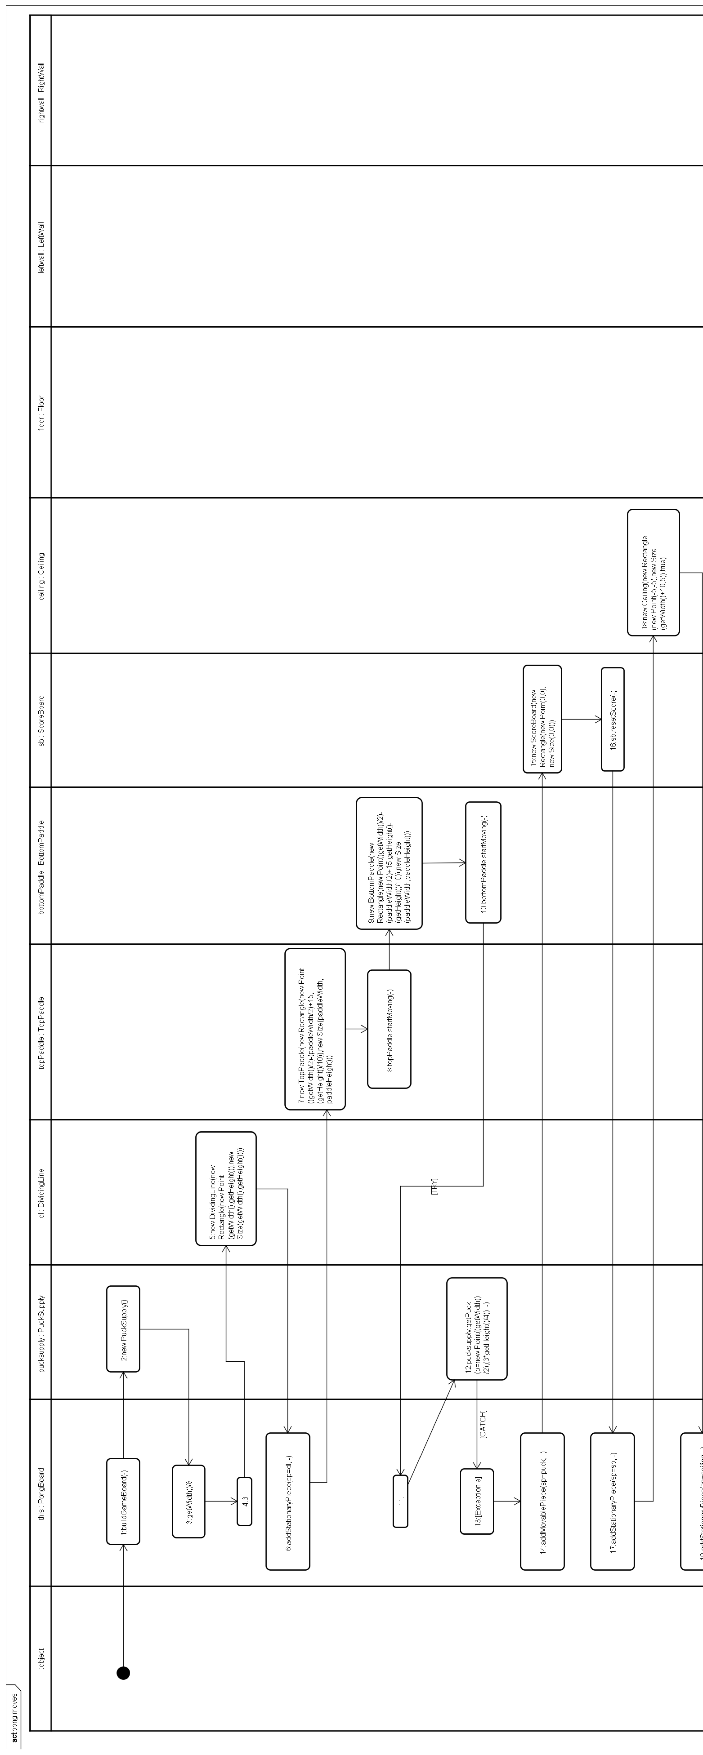
\includegraphics[scale=0.61]{3_pong_moves_DS_to_DA1.pdf}
		\caption{Diagrama de Atividades resultante do Diagrama de Sequência da \ref{fig:pong_movesKleber1} e da \ref{fig:pong_movesKleber2} parte 1}
		\label{fig:pong_movesDS_to_DA1}
	\end{figure}
%\end{landscape}
\begin{landscape}
	\begin{figure}[H]
		\centering
		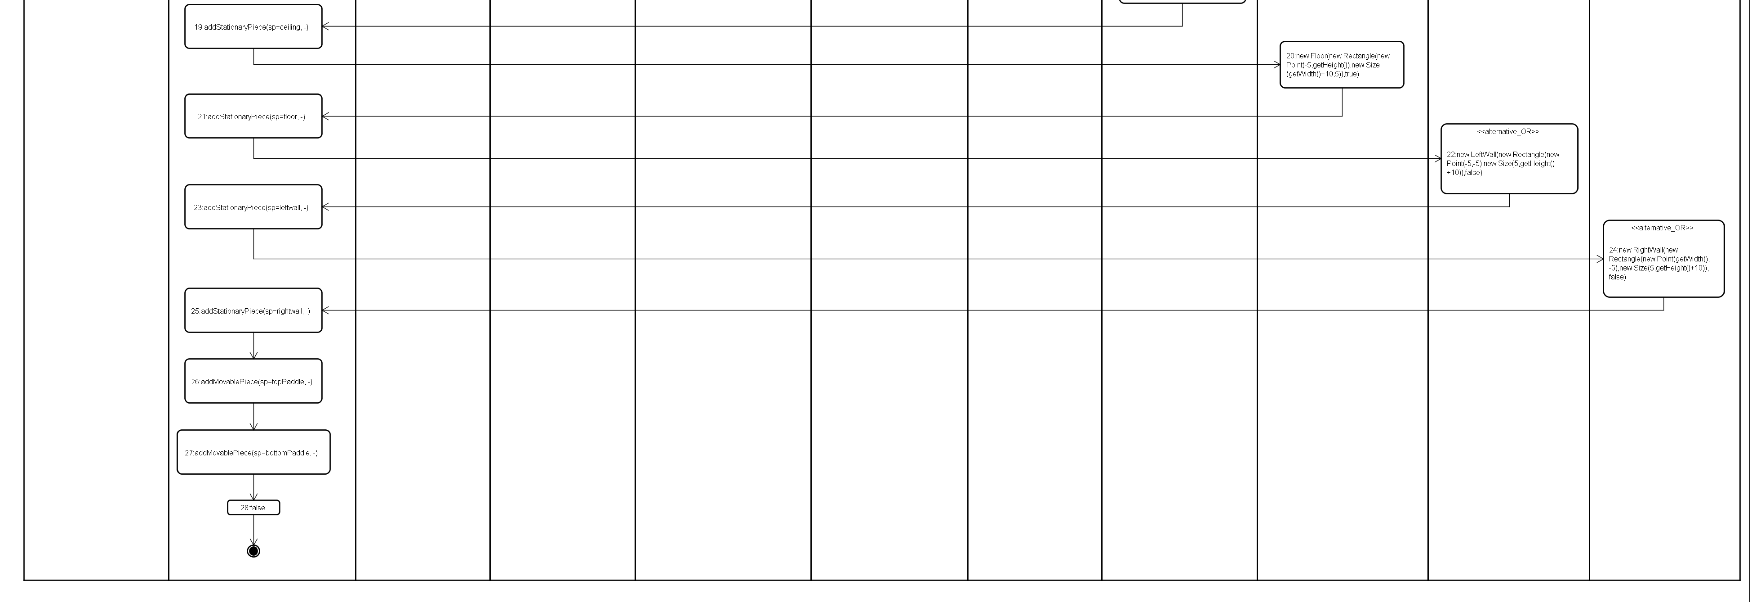
\includegraphics[scale=0.70]{3_pong_moves_DS_to_DA2.pdf}
		\caption{Diagrama de Atividades resultante do Diagrama de Sequência da \ref{fig:pong_movesKleber1} e da \ref{fig:pong_movesKleber2} parte 2}
		\label{fig:pong_movesDS_to_DA2}
	\end{figure}
\end{landscape}
%\end{landscape}



\begin{landscape}
	\begin{longtable}{c|c|l|l}
		\caption{Sequências de teste do DA da \ref{fig:pong_movesDS_to_DA1} geradas por \textit{SMartyTesting}}
		\label{tab:pong_movesDS_to_DA}\\
		\hline
		\textbf{\begin{tabular}[c]{@{}c@{}}Sequência \\ de Teste\end{tabular}} & \textbf{Passo} & \textbf{Ação/Descrição} & \textbf{Resultado Esperado} \\ \hline
		\endhead
		%
		\textit{Test Case} 1 & 1 & \begin{tabular}[c]{@{}l@{}}\textit{buildGameBoard}(-)\\ - método \textit{buildGameBoard} chamado;\end{tabular} & \begin{tabular}[c]{@{}l@{}}recebe parâmetro \\ de inicialização.\end{tabular} \\ \hline
		\textit{Test Case} 1 & 2 & \begin{tabular}[c]{@{}l@{}}\textit{new PuckSupply}()\\ - instancia do método \textit{newPuckSupply};\end{tabular} & método iniciado. \\ \hline
		\textit{Test Case} 1 & 3 & \begin{tabular}[c]{@{}l@{}}\textit{getWidth}()/8\\ - \textit{getWidth}()/;\end{tabular} & captura do tamanho. \\ \hline
		\textit{Test Case} 1 & 4 & \begin{tabular}[c]{@{}l@{}}3\\ - \textit{return};\end{tabular} & retornar valor. \\ \hline
		\textit{Test Case} 1 & 5 & \begin{tabular}[c]{@{}l@{}}- \textit{new DividingLine(new Rectangle(new Point(getWidth()}\\ ,\textit{getHeight()}),\textit{new Size(getWidth(),getHeight()})))\end{tabular} & \begin{tabular}[c]{@{}l@{}}tamanho dos \\ objetos definidos.\end{tabular} \\ \hline
		\textit{Test Case} 1 & 6 & - \textit{addStationaryPiece}(sp=dl, -) & \begin{tabular}[c]{@{}l@{}}complementos \\ adicionados.\end{tabular} \\ \hline
		\textit{Test Case} 1 & 7 & \begin{tabular}[c]{@{}l@{}}- \textit{new TopPaddle(new Rectangle(new Point((getWidth()/2)}\\ -(\textit{paddleWidth}/2) 15,(\textit{getHeight}()/10)),\textit{new} \\ \textit{Size(paddleWidth,paddleHeight)}))\end{tabular} & \begin{tabular}[c]{@{}l@{}}posição dos \\ objetos definidos.\end{tabular} \\ \hline
		\textit{Test Case} 1 & 8 & - \textit{topPaddle.startMoving}(-) & \begin{tabular}[c]{@{}l@{}}\textit{paddle} permite \\ movimentos.\end{tabular} \\ \hline
		\textit{Test Case} 1 & 9 & \begin{tabular}[c]{@{}l@{}}- \textit{new BottomPaddle(new Rectangle(new Point((getWidth()/2)}\\ -(\textit{paddleWidth}/2) 15,\textit{getHeight}()-(\textit{getHeight}()/10)),\\ \textit{new Size(paddleWidth,paddleHeight)}));\end{tabular} & \begin{tabular}[c]{@{}l@{}}posição dos \\ objetos definidos.\end{tabular} \\ \hline
		\textit{Test Case} 1 & 10 & - \textit{topPaddle.startMoving}(-); & \begin{tabular}[c]{@{}l@{}}\textit{paddle} permite \\ movimentos.\end{tabular} \\ \hline
		\textit{Test Case} 1 & 11 & \begin{tabular}[c]{@{}l@{}}11:\\ - \textit{return};\end{tabular} & \begin{tabular}[c]{@{}l@{}}verifica posição \\ e movimento.\end{tabular} \\ \hline
		\textit{Test Case} 1 & 12 & \begin{tabular}[c]{@{}l@{}}- \textit{pucksupply.getPuck(p=new Point((getWidth()/2)},\\ (3*\textit{getHeight}()/4)), -);\end{tabular} & \begin{tabular}[c]{@{}l@{}}se objeto cruzou \\ posição realiza a busca.\end{tabular} \\ \hline
		\textit{Test Case} 1 & 13 & - {[}\textit{Exception} e{]}; & \begin{tabular}[c]{@{}l@{}}situação tratada \\ dispara próximo método.\end{tabular} \\ \hline
		\textit{Test Case} 1 & 14 & - \textit{addMovablePiece(sp=puck, -)}; & adiciona novo objeto móvel. \\ \hline
		\textit{Test Case} 1 & 15 & \begin{tabular}[c]{@{}l@{}}- \textit{new ScoreBoard(new Rectangle(new Point(0,0)},\\ \textit{new Size}(0,0)));\end{tabular} & \begin{tabular}[c]{@{}l@{}}objeto criado na \\ posição determinada.\end{tabular} \\ \hline
		\textit{Test Case} 1 & 16 & - sb.\textit{resetScore}(-); & valor da variável resetada. \\ \hline
		\textit{Test Case} 1 & 17 & - \textit{addStationaryPiece}(sp=sb, -); & \begin{tabular}[c]{@{}l@{}}adiciona novo \\ objeto estacionário.\end{tabular} \\ \hline
		\textit{Test Case} 1 & 18 & \begin{tabular}[c]{@{}l@{}}- \textit{new Ceiling(new Rectangle(new Point(-5,-5)},\\ \textit{new Size(getWidth() 10,5)),true)};\end{tabular} & \begin{tabular}[c]{@{}l@{}}objeto criado na \\ posição determinada.\end{tabular} \\ \hline
		\textit{Test Case} 1 & 19 & \begin{tabular}[c]{@{}l@{}}- \textit{new Floor(new Rectangle(new Point(-5,getHeight())},\\ \textit{new Size(getWidth() 10,5)),true)};\end{tabular} & \begin{tabular}[c]{@{}l@{}}adiciona novo objeto \\ estacionário no teto.\end{tabular} \\ \hline
		\textit{Test Case} 1 & 20 & - \textit{addStationaryPiece(sp=floor, -)}; & \begin{tabular}[c]{@{}l@{}}objeto criado na \\ posição determinada.\end{tabular} \\ \hline
		\textit{Test Case} 1 & 21 & \begin{tabular}[c]{@{}l@{}}VP\_21:\textit{addStationaryPiece}(sp=\textit{floor}, -)\\ - \{;\\ - \textit{new LeftWall}(\textit{new Rectangle(new Point(-5,-5)},\\ \textit{new Size}(5,\textit{getHeight}() 10)),\textit{false})\{\textit{alternative\_OR}\}\};\end{tabular} & \begin{tabular}[c]{@{}l@{}}adiciona novo objeto\\  estacionário na base.\end{tabular} \\ \hline
		\textit{Test Case} 1 & 22 & \begin{tabular}[c]{@{}l@{}}- \{;\\ - \textit{addStationaryPiece(sp=leftwall, -)}\};\end{tabular} & \begin{tabular}[c]{@{}l@{}}\{.\\ objeto criado na \\ posição determinada\}.\end{tabular} \\ \hline
		\textit{Test Case} 1 & 23 & \begin{tabular}[c]{@{}l@{}}VP\_23:\textit{addStationaryPiece(sp=leftwall, -)}\\ - \{;\\ - \textit{new RightWall(new Rectangle(new Point(getWidth(),-5)},\\ \textit{new Size(5,getHeight()} 10)),\textit{false})\{\textit{alternative\_OR}\}\};\end{tabular} & \begin{tabular}[c]{@{}l@{}}\{.\\ adiciona novo objeto \\ estacionário parede esquerda\}.\end{tabular} \\ \hline
		\textit{Test Case} 1 & 24 & \begin{tabular}[c]{@{}l@{}}VP\_23:\textit{addStationaryPiece}(sp=\textit{leftwall}, -)\\ - \{;\\ - \textit{new RightWall(new Rectangle(new Point(getWidth(),-5)},\\ \textit{new Size(5,getHeight() 10)),false)\{alternative\_OR\}}\};\end{tabular} & \begin{tabular}[c]{@{}l@{}}\{.\\ objeto criado na \\ posição determinada\}.\end{tabular} \\ \hline
		\textit{Test Case} 1 & 25 & \begin{tabular}[c]{@{}l@{}}- \{;\\ - \textit{addStationaryPiece(sp=rightwall, -)}\};\end{tabular} & \begin{tabular}[c]{@{}l@{}}\{.\\ adiciona novo objeto \\ estacionário parede direita\}.\end{tabular} \\ \hline
		\textit{Test Case} 1 & 26 & - \textit{addMovablePiece(sp=topPaddle, -)}; & \begin{tabular}[c]{@{}l@{}}adiciona novo objeto móvel \\ ao \textit{paddle} posição \textit{top}.\end{tabular} \\ \hline
		\textit{Test Case} 1 & 27 & - \textit{addMovablePiece(sp=bottomPaddle, -)}; & \begin{tabular}[c]{@{}l@{}}adiciona novo objeto móvel \\ ao \textit{paddle} posição \textit{bottom}.\end{tabular} \\ \hline
		\textit{Test Case} 1 & 28 & \begin{tabular}[c]{@{}l@{}}\textit{false}\\ - \textit{return false};\end{tabular} & \begin{tabular}[c]{@{}l@{}}caso retorne \textit{false} para \\ ações encerra sessão.\end{tabular} \\ \hline
	\end{longtable}
\end{landscape}


\section{Análise e Interpretação}
\label{cap4sec:analiseeinterpretacao}

\subsection{Quantidade de Sequências de Teste Geradas (CT.1)}
%Foram utilizados três modelos da LPS AGM, onde foram modelados primeiramente o caso de uso e em seguida o diagrama base para utilização na abordagem de geração de caso de teste, para SPLiT-MBt foi utilizado o diagrama de atividade \cite{costa2016split} e para \textit{SMartyTesting} o diagrama de sequência \cite{marcolino2013towards}.

%Na Seção \ref{cap4sec:execucaocomparativo} é apresentado todos os artefatos utilizados, assim como as sequências de casos de teste gerados, onde, tais dados são utilizados nessa análise.

Na \ref{tab:comparacaoDSxDA} são apresentados os números da geração de sequências de teste de abordagem e também a soma de todas as sequências de teste geradas conforme o diagrama usado.

\begin{table}[H]
	\centering
	\caption{Quantidade de sequências de teste geradas por abordagem.}
	\label{tab:comparacaoDSxDA}
	\begin{tabular}{l|c|c}
		\hline
		\multicolumn{1}{c|}{\textbf{Diagrama}} & \textbf{SMartyTesting (DS)} & \textbf{SPLiT-MBt (DA)} \\ \hline
		\textit{Play Selected Game} & 6 & 5 \\ \hline
		\textit{Save Game} & 12 & 6 \\ \hline
		\textit{Pong Moves} & 28 & 3 \\ \hline
		\multicolumn{1}{c|}{\textbf{Total de sequências de teste}} & \textbf{46} & \textbf{14} \\ \hline
	\end{tabular}
\end{table}

Com base nesses dados, pode-se identificar que quando utilizados DS a quantidade de sequências de teste tende a ser consideravelmente maior. Entende-se, dessa forma, que isso possa ser determinado pelo nível de abstração do diagrama: quanto mais abstrato, menor a quantidade de casos de teste.

Se for considerado o nível de abstração de cada diagrama, com esses dados é possível fornecer evidências iniciais de que diagramas de sequência possuem potencial para a geração de maior quantidade de sequências de teste. Portanto, pode-se aceitar a hipótese $H_{CT.1}$, o que significa que há evidência de que \textit{SMartyTesting} é viável para geração de um número maior de sequências de teste utilizando DSs.

\subsection{Diferença entre as Sequências Geradas (CT.2)}
Ao se observar os artefatos de entrada, em que suas semelhanças se fazem por equivalência, identifica-se que existe diferença entre as sequências geradas, isso já mencionado anteriormente, e se deve ao fato de nível de abstração.

Embora DS e DA sejam diagramas de comunicação, existe aplicabilidade diferenciada para cada um deles e, por DS estar mais próximo do código fonte, é de se esperar que as sequências geradas diferem de um modelo alto nível, porém, em determinados modelos as sequências quase se equivalem. Entende-se, portanto, que isso depende do nível de detalhamento que o engenheiro de software aplica ao modelo DS.

\subsection{Complexidade na Geração de Sequências de Teste (CT.3)}
\label{cap4subsec:ciclomatico}
Para determinar a complexidade da geração foi utilizada a métrica de complexidade ciclomática de \citet{mccabe1976complexity}. 


Para essa viabilidade foram encontrados mais estudos que utilizam e fazem análise de complexidade ciclomática, \cite{jay2009cyclomatic,gill1991cyclomatic,shepperd1988critique}, porém, todos fazem utilização do mesmo conceito primário abordado por \citet{mccabe1976complexity}. Por isso optou-se por seguir os conceitos primários para a utilização da complexidade ciclomática. 

Tal métrica serve para mensurar a complexidade de um determinado módulo (uma classe, um método, uma função etc.), a partir da contagem do número de caminhos independentes que o modelo pode executar até o seu fim. Um caminho independente é aquele que apresenta pelo menos uma nova condição (possibilidade de desvio de fluxo) ou um novo conjunto de comandos a serem executados.


Tendo um grafo de fluxo, tem-se três fórmulas equivalentes para se mensurar a complexidade ciclomática  \citet{mccabe1976complexity}:
\begin{enumerate}
	\item V(G) = R, em que R é o número de regiões do grafo de fluxo;
	\item V(G) = E – N + 2, em que E é o número de arestas (setas) e N é o número de nós do grafo G;
	\item V(G) = P + 1, em que P é o número de nós-predicados contidos no grafo G (só funciona se os nós-predicado tiverem no máximo duas arestas saindo.)
\end{enumerate}

A \ref{tab:ciclomatico_gerado} apresenta os dados utilizando a fórmula número 2.

\begin{table}[H]
	\centering
	\caption{Parâmetros aceitáveis para a complexidade ciclomática}
	\label{tab:ciclomaticotabelarisco}
	\begin{tabular}{c|l}
		\hline
		\textbf{Complexidade} & \multicolumn{1}{c}{\textbf{Avaliação}} \\ \hline
		1-10 & Método simples. \textbf{Baixo risco} \\ \hline
		11-20 & Método razoavelmente complexo. \textbf{Moderado risco} \\ \hline
		21-50 & Método muito complexo. \textbf{Elevado risco} \\ \hline
		51-N & Método de \textbf{altíssimo risco} e bastante instável \\ \hline
	\end{tabular}
\end{table}

Após a análise dos grafos gerados por ambos os DA utilizados na geração de sequências de teste obteve-se a \ref{tab:ciclomatico_gerado}. Nela pode-se perceber que a complexidade diferentemente da quantidade de sequências geradas, quase se equivale baseado na \ref{tab:ciclomaticotabelarisco}. Outro fator é a complexidade dos artefatos, que se manteve como simples e de baixo risco, o que é muito bom.

\begin{table}[H]
	\centering
	\caption{complexidade ciclomática apresentada pelas abordagens}
	\label{tab:ciclomatico_gerado}
	\begin{tabular}{l|c|c}
		\hline
		\multicolumn{1}{c|}{\textbf{Diagrama}} & \textbf{\textit{SMartyTesting} (DS)} & \textbf{SPLiT-MBt (DA)} \\ \hline
		\textit{Play Selected Game} & 3 & 4 \\ \hline
		\textit{Save Game} & 3 & 2 \\ \hline
		\textit{Pong Moves} & 1 & 1 \\ \hline
		\multicolumn{1}{c|}{\textbf{Total}} & \textbf{7} & \textbf{7} \\ \hline
	\end{tabular}
\end{table}

Pode-se concluir que, embora diagramas DS possuam maior nível de detalhes, se usados por \textit{SMartyTesting} possuem complexidade menor se comparados com DA utilizado por SPLiT-MBt, que possui nível maior de abstração.


\subsection{Esforço na Utilização das Abordagens (CT.4)}
Outro critério de análise é o de esforço na utilização das abordagens. Para isso, levou-se em consideração o tempo utilizado para a realização do ciclo de geração completo, da entrada do artefato inicial DS para \textit{SMartyTesting} e DA para SPLiT-MBt até a geração de sequência de teste.

Considera-se que para ser observado o esforço, parte-se de que os diagramas DS e DA, ambos artefatos de entrada para cada uma das abordagens observadas, já estejam modelados.

Então, é dado início ao processo de geração de sequência para cada abordagem, \textit{SMartyTesting} com diagramas de sequência e SPLiT-MBt com o diagrama de atividades. Por não possuir ainda todo seu processo automatizado, \textit{SMartyTesting} se torna uma abordagem que demanda esforço maior em sua utilização e compreensão, vide o mapeamento manual que deve ser feito de DS para DA.

Embora \textit{SMartyTesting} utilize SPLiT-MBt, \textit{SMartyTesting} demanda mais esforço em sua primeira etapa, para a realização da conversão manual de DS para DA, o que pode ser amenizado com implementações futuras.

Em trabalhos futuros a recomendação é que seja feita conversão automática direta de DS para MEF, garantindo assim maior performance e menor redundância de dados.

\section{Ameaças à Validade}
Nesta seção são tratadas as ameaças e ações tomadas para amenizar alguns dos problemas encontrados durante a execução deste estudo, incluindo ameaças à validação interna, externa, de \textit{constructo} e de conclusão.

\subsection{Validade Interna}

Tem a intenção de verificar se a comparação das gerações de sequências de teste realmente obtiveram os resultados esperados, dado que a seguinte ameaça foi identificada:

\textbf{Método de conversão manual de DS para DA:} por ser o principal item de diferenciação entre \textit{SMartyTesting} e SPLiT-MBt, a conversão do artefato DS para DA feita de forma manual, pode gerar um viés em relação à aplicação das regras de mapeamento, devido ao processo de conversão não ser automatizado. Podendo induzir a erros de modelagem durante a criação do diagrama de atividades. Para contornar esse viés, durante a comparação de viabilidade, foram seguidos sistematicamente todos os itens da \ref{tab:regrasmapeamento} do mapeamento proposto por \citet{garousi2005control}.

\subsection{Validade Externa}
\textbf{Autores especialistas:} a interpretação das funcionalidades no momento da modelagem pode influenciar no nível de complexidade do diagrama de DS e DA. Para poder realizar o estudo de viabilidade amenizando esse viés foram selecionados dois autores que são doutores além de já dominarem o assunto abordado neste trabalho. 

\subsection{Validade de \textit{Constructo}}

Pelo fato de a conversão ser feita de forma manual, mesmo sendo realizada com base em um conjunto de regras de mapeamento \cite{garousi2005control} pode gerar questionamentos sobre as funcionalidades representadas. 

Para amenizar esse viés, foi analisado se o mapeamento já havia sido validado, nesse caso por \citet{shafique2010systematic}, que apresentam uma abordagem de geração de casos de teste a partir de diagramas de sequência. 

\subsection{Validade de Conclusão}
Este trabalho é um estudo inicial de viabilidade, não sendo possível generalizar os resultados.

\section{Considerações Finais}
Os resultados obtidos por comparações e observações de utilização das duas abordagens, permitiram avaliar a viabilidade da abordagem \textit{SMartyTesting} além de propor possíveis melhorias para a abordagem SPLiT-MBt.

Além de viabilizar estudos futuros para implementação de ferramentas de apoio, que façam utilização dos conceitos da abordagem \textit{SMartyTesting}, no próximo tópico são apresentadas todas as melhorias identificadas e lições aprendidas com a pesquisa.




% Tópico 5 
\chapter{Melhorias Identificadas e Lições Aprendidas }
\label{cap5:melhorias}
\pagestyle{plain}

\section{Considerações Iniciais}
Com base no estudo realizado no tópico \ref{cap4:avaliacao} e os seus resultados, foram identificadas algumas melhorias e lições aprendidas sobre ambas as abordagens \textit{SMartyTesting} e SPLiT-MBt.

As melhorias são fundamentais para guiar trabalhos futuros relacionados à esta dissertação. Lições aprendidas são discutidas com o intuito de transferir o máximo possível de conhecimento adquirido com este trabalho.


\section{Melhorias Identificadas}
\label{cap5sec:melhorias_melhorias}
As melhorias identificadas estão voltadas tanto para \textit{SMartyTesting} como para SPLiT-MBt. Tais sugestões foram analisadas e são discutidas a seguir.

\subsection{Automatização do Processo de Geração de Sequências de Teste}
Na Seção \ref{cap4sec:analiseeinterpretacao} foi possível a análise da viabilidade de utilização de \textit{SMartyTesting}. Embora evidenciado que exista viabilidade na sua utilização, um fator observado é o nível de esforço que a abordagem necessita para a geração de sequências de teste, o que não ocorre em SPLiT-MBt uma vez que todo o processo é automatizado.

Nesse caso a melhoria pontual seria a implementação completa do processo de teste usando \textit{SMartyTesting}, partindo do modelo de entrada (DS), convertendo o DS para MEF e, então, gerando as sequências de teste, utilizando SPLiT-MBt como base ou uma nova implementação com uma estrutura própria. 

Partindo de uma implementação nova, pode-se garantir um código mais ajustado ao propósito da abordagem, sem dependências de códigos não utilizados ou sistemas legados sem suporte. Aqui três pontos devem ser tratados:

\begin{itemize}
	\item a conversão de DS para MEF;
	\item a implementação ou adaptação de um dos algoritmos apresentados na Seção \ref{cap2subsec:metodo_geracao}; e
	\item a geração das sequências de teste.
\end{itemize}

Caso seja considerada a adaptação da SPLiT-MBt nessa nova implementação, dois itens devem ser tratados: 

\begin{itemize}
	\item suporte a \textit{fork node} e \textit{join node}, e
	\item suporte a subsistema com mais de um início ou fim.
\end{itemize}

\subsection{Utilização da Conversão de DS para MEF em \textit{SMartyTesting}}
Para a realização da automatização de todo o ciclo de \textit{SMartyTesting}, o ideal é que algumas mudanças com relação ao seu processo de conversão sejam realizadas. Embora a utilização de SPLiT-MBt por \textit{SMartyTesting} seja viável, estudos preliminares contidos no MSL (Apêndice \ref{sec:secmsl_MSL}) demonstram que a diminuição de etapas torna o processo de teste mais objetivo e confiável em nível de falhas ocasionadas por erros básicos.

Assim como SPLiT-MBt faz o uso de MEFs, a recomendação seria que \textit{SMartyTesting} também fizesse uso do mesmo artefato, pois MEF está entre os modelos formais mais utilizados em TBM de LPS. Além disso, MEF é uma boa alternativa para projetar componentes de teste de software, pois pode ser aplicada a qualquer modelo de especificação que descreva um número finito de etapas \cite{costa2016split}.

Outro ponto de análise é que para gerar uma quantidade considerável de sequências de teste sobre um modelo, o ideal é a utilização de métodos de geração de sequências de teste. Para que isso seja possível, a utilização de MEF é a solução mais adequada. Porém, assim como \citet{costa2016split}, deve-se também aprimorar uma extensão para que MEF possa representar informações de variabilidade, visto que MEF foi projetada essencialmente para testar softwares com base no paradigma de desenvolvimento de sistema único. 

\subsection{Suporte para Programação Concorrente e Sub-processo em SPLiT-MBt}
\label{cap5sec:limitacaoconcorrencia}
Foram encontradas duas situações em que SPLiT-MBt se torna limitante, a primeira delas é em relação às chamadas de fluxo concorrente, que utilizam um \textit{Fork Node} diferente de um \textit{Node Decision} que só possui um caminho. Representando \textit{if} ou \textit{else}, o \textit{Fork Node} representa uma ação disparada que pode ser direcionada a dois estados ao mesmo tempo, como exemplificado na \ref{fig:mapeamento4}.

Um exemplo seria a conversão do diagrama da \ref{fig:dslimitacao}, em que as mensagens seis e sete são assíncronas, disparando o processo e dando continuidade ao fluxo principal.

\begin{figure}[H]
	\centering
	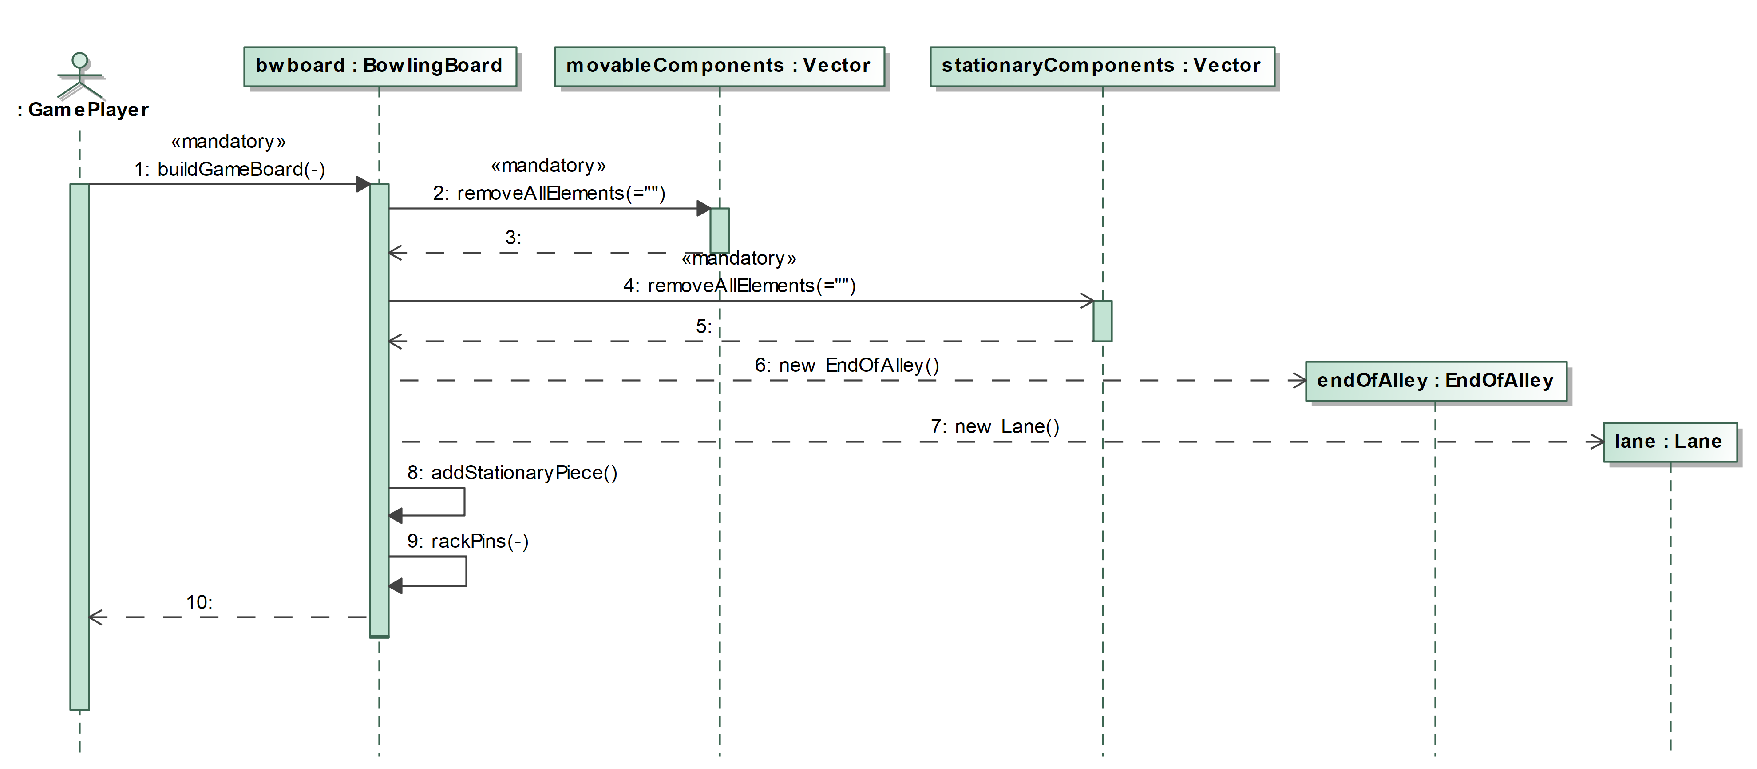
\includegraphics[width=\textwidth]{DSlimitacao.pdf}
	\caption{Exemplo de DS com mensagens representando  programação concorrente em uma função de \textit{login}}
	\label{fig:dslimitacao}
\end{figure}

No DA convertido, essas mensagens seis e sete, iriam partir de um \textit{Fork Node} e, após isso, poderiam ser representadas como um subprocesso ou um \textit{End Node} (\ref{fig:dalimitacao}).

\begin{figure}[H]
	\centering
	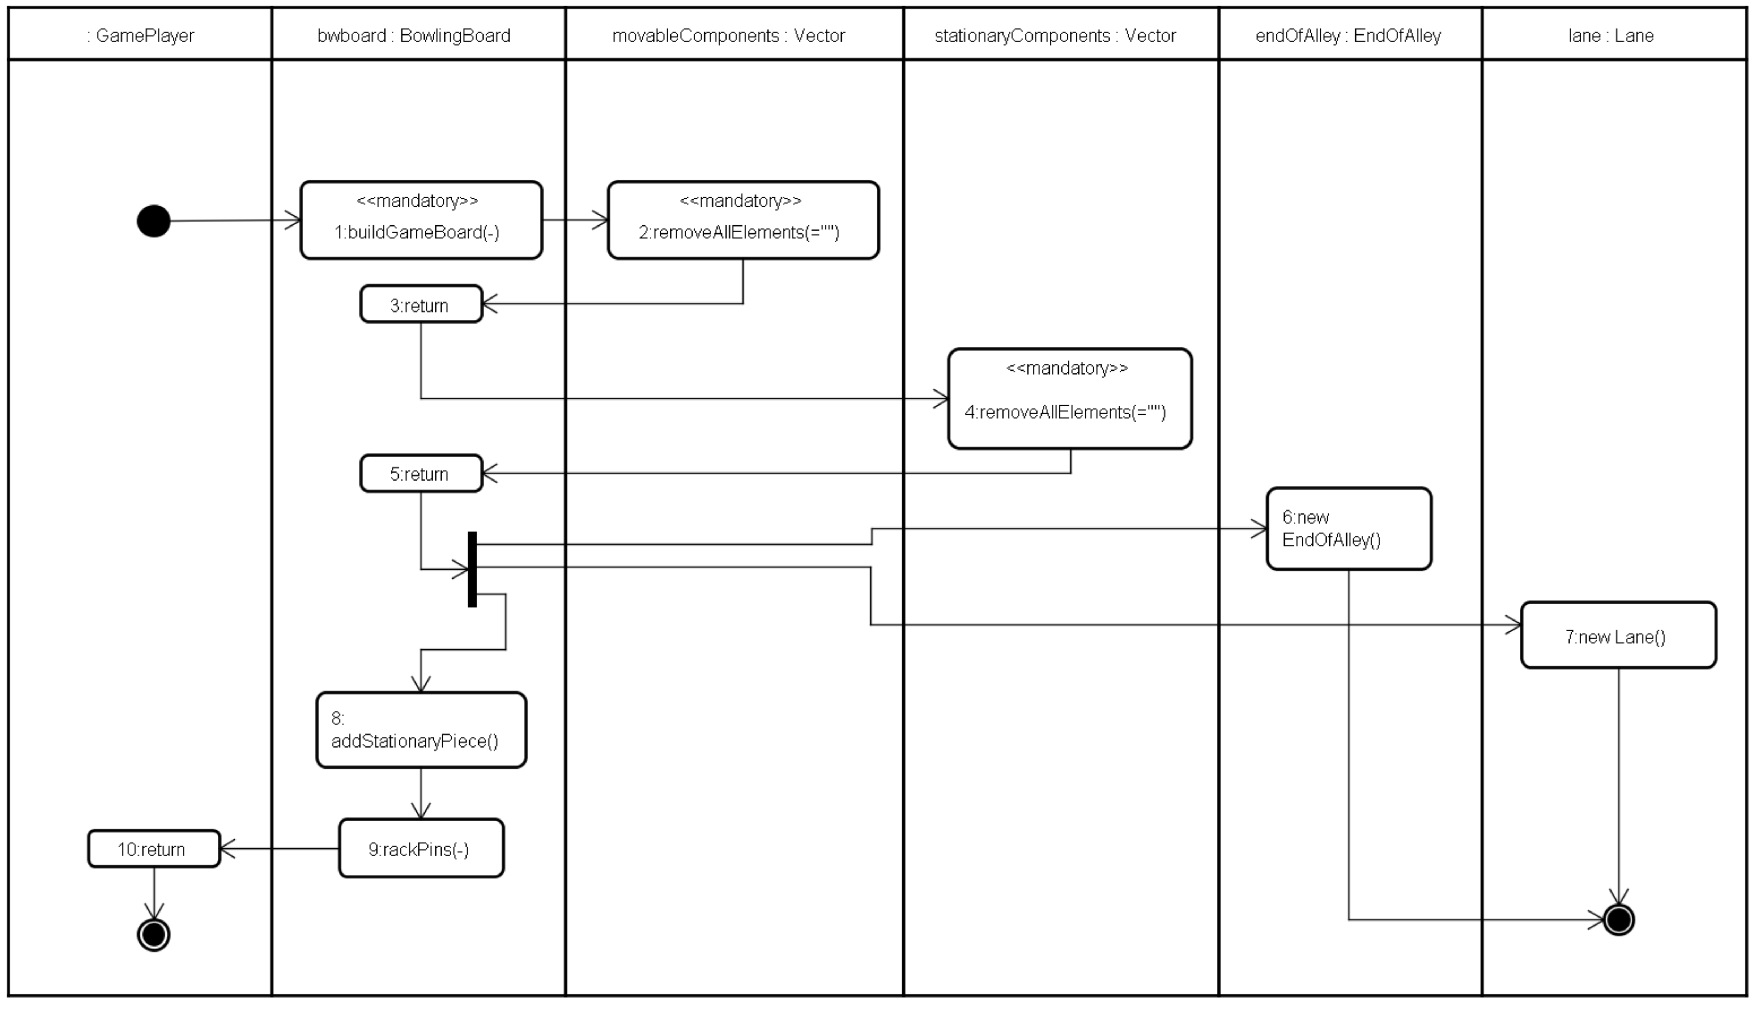
\includegraphics[width=\textwidth]{DAlimitacao.pdf}
	\caption{DA com mensagens representando programação concorrente em uma função de \textit{login}}
	\label{fig:dalimitacao}
\end{figure}

Como o DA não possui suporte ao \textit{Fork Node}, consequentemente, não possui suporte também ao \textit{Join Node}, que faz a junção de fluxo vindo de objetos diferentes. Além disso, fica visível a necessidade de suporte também a subsistemas em que um modelo possui mais de um elemento de \textit{Initial Node} ou \textit{End Node}. Quando se trabalha com subsistemas pode haver a finalização de um subprocesso para dar continuidade no processo principal, exemplificado na \ref{fig:mapeamento4}.

\subsection{Suporte para Outro Métodos de Geração de Sequências de Teste}
Na Seção \ref{cap2subsec:metodo_geracao} foram abordados os métodos de geração de sequências de teste. SPLiT-MBt faz utilização do método HSI, em que \citet{costa2016split} justifica que tal método é o menos restritivo com relação às propriedades na utilização em LPS.

\citet{pinheiro2012jplavisfsm}, no entanto citam que se deve levar em conta a relação custo-benefício de cada método, pois o foco principal consiste em promover a detecção do maior número possível de defeitos existentes em uma implementação, levando em conta o tamanho do conjunto gerado, para que esse fato não inviabilize a sua aplicação prática. \citet{pinheiro2012jplavisfsm} realizaram um trabalho de geração de sequências com os métodos de geração mais utilizados, como visto na Seção \ref{cap2subsec:plavis}.

Embora \citet{costa2016split} tenha feito ensaios demonstrando que o HSI produz melhores resultados, a sugestão seria a implementação dos demais métodos como opção de geração de sequências de teste para SPLiT-MBt, deixando a cargo do engenheiro de software selecionar qual o método de geração é mais efetivo ao objetivo almejado.

\section{Lições Aprendidas}
\label{cap5sec:licoes_aprendidas}
\subsection{Compreensão de SPLiT-MBt}
A abordagem SPLiT-MBt contribuiu muito para o entendimento da geração de sequências de teste e o entendimento sobre a estrutura necessária para a geração das sequências.

Adaptação de métodos de geração de sequência a partir de modelos formais como MEF foram itens fundamentais para a visualização de trabalhos futuros relacionados à geração de sequências de teste fazendo uso de outros métodos de geração.

Embora a ferramenta seja caixa preta, uma boa documentação com todos os parâmetros bem explicados se faz necessária, ficando o aprendizado de todo o processo, desde o artefato de entrada até as sequências de teste geradas, explicado na Seção \ref{cap2sec:split_abordagem}. Dessa forma, a lição aprendida é a necessidade de disponibilidade das implementações das abordagens e dos dados obtidos para que a pesquisa possa ser reproduzida.

\subsection{Conversão Manual de DS para DA}
A conversão manual proporcionou aprendizado sobre os metamodelos de DS e DA \textit{Control Flow Analysis of UML 2.0 Sequence Diagrams} possui regras claras, definidas e baseadas no metamodelo de cada diagrama. Isso contribuiu diretamente para o entendimento das conversões dos elementos, embora precise de aprimoramento (extensão) com relação a elementos de variabilidade.

Por mais que não influencie diretamente neste trabalho, o processo de automatização da abordagem \textit{SMartyTesting} contribui para maior confiabilidade e consistência das gerações de sequências de teste. 
\subsection{ATLs para Conversão}
Por causa do grande aumento da complexidade no desenvolvimento de software nos últimos anos, academia e indústria criaram uma solução racional na engenharia de software, chamada de Engenharia Dirigida por Modelos, que busca apoiar o gerenciamento de tal complexidade. Uma operação importante na Engenharia Dirigida por Modelos é a transformação de modelos, que consiste em um processo automatizado de conversão de um modelo origem para um modelo de destino \cite{allilaire2006atl}.

Durante o processo de pesquisa foram encontradas duas ATLs de conversão de DS para \textit{Statechart} e outra de DS para MEF, em que a primeira \textit{UML Sequence Diagrams to Statechart Diagram} \footnote[1]{Disponível em:http://www.st.ewi.tudelft.nl/basgraaf/ - Acessado em 20/03/2019} possui documentação de utilização extremamente confusa e de difícil configuração e, para tanto, foram realizados testes de conversão de diagramas de exemplos que estavam disponíveis no pacote, mas não foi obtido o resultado esperado. A segunda, também \textit{open-source}, é chamada de \textit{Convert UML Sequence Diagram to UML State Machine} \footnote[2]{Disponível em: https://github.com/slashburn/mdd-project - Acessado em 10/04/2019} que possui documentação um pouco mais detalhada em comparação a anterior. Foram realizados testes iniciais com os exemplos contidos no pacote onde houve êxito de conversão com alguns diagramas \cite{hennicker2007activity}.

Ambas as ATLs dispõem de pacotes que utilizam uma linguagem de conversão \textit{Query/View/Transformation} (QVT). QVT é uma linguagem utilizada para transformar (meta) modelos e usa OCL (\textit{Object constraint language}) estendida em combinação com uma linguagem específica de domínio: Relações, Core ou Operacional. Este último é uma linguagem imperativa, enquanto as outras duas são declarativas e ambas dependem do IDE Eclipse.

\textit{Convert UML Sequence Diagram to UML State Machine} possui suporte a arquivos com extensão ``.UML", sendo assim, a quantidade de ferramentas que poderiam auxiliar na concepção de diagramas que pudessem ser convertidos ficou limitada, por causa de outras existentes utilizarem formatos próprios de saída. Em princípio, não foi realizada busca por conversões de formato para obter abrangência maior, em vez disso, procurou-se uma ferramenta que fosse robusta e pudesse entregar o proposto. Sendo assim, optou-se por realizar testes como a \textit{UML Designer}\footnote[3]{Disponível em: http://www.umldesigner.org/download/ - Acessado em 10/04/2019} embora, sem sucesso também.

Por fim, a experiência com ATLs de conversão de DS para MEF não foi satisfatória por causa das complexidades de utilização, curva de aprendizado e pouca documentação, o que reforça a lição aprendida anteriormente.

\subsection{Uso de Ferramentas}
O uso de ferramentas se faz necessário para a automatização dos processos ou até mesmo para apoio à criação de diagramas. Houve dificuldades em relação à curva de aprendizagem e documentação das ferramentas pesquisadas para validação, como, por exemplo, JPlavisFSM, \textit{Control Flow Analysis of UML 2.0 Sequence Diagrams} e SPLiT-MBt.

Outro fator de aprendizado são os níveis de configuração e disponibilização das ferramentas, \textit{links} quebrados, informações falhas sobre locais para \textit{download}, principalmente qual a versão da ferramenta utilizada. Esses são os exemplos de aprendizado obtido com relação às ferramentas utilizadas. 
\subsection{Teste Baseado em Modelos de LPS}
O processo TBM para LPS que foi vivenciado demonstra de fato o que é apresentado no Apêndice \ref{sec:secmsl_MSL}, processos similares, assim como as dificuldades e desafios. 

TBM se apresenta como uma forma bem estruturada de técnica de teste voltada para utilização em LPS, por ser adaptável e flexível em seus processos.

\section{Considerações Finais}
O trabalho de viabilidade de \textit{SMartyTesting} permitiu a validação de SPLiT-MBt em pontos importantes, essa validação contribuiu direta e indiretamente para a incorporação do conceito de SPLiT-MBt em \textit{SMartyTesting}.

Nas melhorias identificadas, além do processo de automatização de \textit{SMartyTesting} e a ampliação do suporte de SPLiT-MBt a novos processos que fazem parte do metamodelo de atividades, permitiram muitas lições aprendidas aos processos apresentados nesse trabalho.


% Tópico 6 
\chapter{Conclusão}
\label{cap6:conclusao}
\pagestyle{plain}

\section{Contribuições}
\label{cap6sec:contribuicoes}

O resultado principal desta pesquisa foi a especificação e a evidência preliminar de viabilidade da abordagem \textit{SMartyTesting} que permite a geração de sequências de teste para LPS considerando variabilidade modelada com suporte da abordagem \textit{SMarty}. \textit{SMartyTesting} tem como artefato de entrada um diagrama de sequência (DS) que possui estrutura definida. Com o objetivo principal de apoiar a cultura de TBM em fases iniciais de LPS, entende-se como uma contribuição a possibilidade de melhorar a qualidade de modelos de LPS.


Sendo assim, após a especificação da abordagem, foi realizado um estudo de viabilidade com alguns critérios de comparação para que fosse possível responder a seguinte questão de pesquisa: \textbf{``Diagramas de sequência podem gerar mais sequências de teste do que diagramas de atividades?"}


A geração de sequências de teste a partir de DS se mostrou viável por apresentar baixa complexidade ciclomática (CT.3) em suas conversões, demonstrando potencial para a sua utilização, o que se alinha aos resultados do MSL realizado.


A quantidade de sequências de teste geradas é maior, conforme esperado, devido a quantidades de atividades geradas a partir do diagrama de sequência (CT.1). Isso impacta diretamente na diferenciação das sequências de teste geradas (CT.2).


Devido a conversão manual de DS para DA, o esforço de utilização (CT.4) se torna maior com \textit{SMartyTesting}, mas isso já se era previsto por ser uma abordagem semi-automatizada.

Além da contribuição principal, considera-se muito importante também a análise da abordagem SPLiT-MBt e de sua ferramenta de apoio. Assim, a Seção \ref{cap5sec:limitacaoconcorrencia} mostra como melhorias podem ser realizadas para as abordagens \textit{SMartyTesting} e SPLiT-MBt contribuindo para a evolução dessas.

O MSL conduzido para a fundamentação desta pesquisa, além de contribuir com dados que apresentam o cenário de TBM para LPS, contribuiu também para a criação de um mapa de direcionamento de estudos relacionados por temas. Tal mapa permite entender como estudos de TBM para LPS têm sido realizados e como pesquisadores e profissionais podem utilizá-los ao tratar deste assunto em pesquisas e práticas na indústria.

Em síntese, buscou-se com o desenvolvimento deste projeto contribuir para a comunidade acadêmica e industrial de LPS com uma abordagem de geração de sequências de teste, que considerem variabilidade na engenharia de domínio e para a engenharia de aplicação de LPS. 

\section{Limitações}
Foram encontradas duas situações em que SPLiT-MBt se torna limitante, a primeira delas é em relação a chamadas de fluxo concorrente, comentado na Seção \ref{cap5sec:limitacaoconcorrencia}, como não possui esse suporte ao \textit{Fork Node}, consequentemente, não possui suporte também ao \textit{Join Node}. Além disso, é visível a necessidade de suporte também a subsistemas em que um modelo possui mais de um elemento de \textit{Initial Node} ou \textit{End Node} estágios de início e fim, dado que quando se trabalha com subsistemas pode haver a finalização de um subprocesso para dar continuidade no processo principal exemplificado na Seção \ref{cap5sec:limitacaoconcorrencia}.

Baseado nesses fatores, pode-se considerar que SPLiT-MBt não tem suporte à mensagens assíncronas, limitando-se apenas a mensagens síncronas em que toda mensagem deve possuir um retorno, não conformante com 100\% do metamodelo da UML.

Quanto às limitações de \textit{SMartyTesting}, é uma abordagem que não converte DS para DA ou para MEF automaticamente, isso é um dos itens que estão considerados como trabalho futuro para a abordagem. Outro item está relacionado ao estudo de viabilidade conduzido com uma amostra pequena de LPS, DS e DA, o que não permite generalizar os resultados obtidos.

\section{Trabalhos Futuros}

Com base na experiência de criação e especificação da abordagem \textit{SMartyTesting}, no processo de comparação e nas observações sobre sua utilização e, visando a continuidade do trabalho que possui um grande potencial, são apresentadas a seguir as principais perspectivas em relação a trabalhos futuros que possam decorrer deste estudo preliminar.

\textbf{Implementação Total para \textit{SMartyTesting}:} após a análise dos dados comparativos e observações realizadas com a abordagem para se ter a certeza que era possível a geração de sequências de teste a partir de DSs, demonstra ser viável a implementação total da abordagem \textit{SMartyTesting}, isso não impede a continuidade da utilização de SPLiT-MBt, que também pode ser incorporada ao processo de \textit{SMartyTesting}.

\textbf{Diminuição das Etapas do Processo:} no MSL foi apontado que diversos trabalhos fazem uso de conversão de DS para MEF, e \citet{pinheiro2012jplavisfsm} apresentam na Seção \ref{cap2subsec:plavis} motivos para a utilização de MEF. Sendo assim, seria interessante em um trabalho futuro analisar a viabilidade do processo de geração de sequências de teste a partir de um DS com conversão direta para MEF e, após essa transformação, utilizar outros métodos de geração de sequências de teste.

\textbf{Incorporar \textit{SMartyTesting} à ferramenta \textit{SMartyModeling}:} em paralelo a este trabalho está sendo desenvolvida outra pesquisa sobre uma ferramenta para modelagem de LPS considerando \textit{SMarty}, em que os diagramas suportados pela versão 5.1 são: sequência, casos de uso, atividades, componentes e classes. Com isso, quando o engenheiro de software fizer a modelagem de uma LPS já tem a possibilidade de gerar das sequências de teste.

\textbf{Aplicar métricas de teste aos modelos \textit{SMarty}:} considerar as métricas de teste no processo de teste e comparar as sequências de teste ou casos de teste em modelos \textit{SMarty}.

\textbf{Estender o perfil de teste da OMG:} estender o perfil de teste da OMG \footnote{Disponível em: \url{https://www.omg.org/spec/UTP} - Acessado em 20/10/2019} \cite{Bagnato_et_al2013} para TBM de LPS, considerando o processo da \textit{SMartyTesting}.   


 



% Fancyhead
\fancyhead[RO,LE]{\itshape REFERÊNCIAS}
\fancyhead[RO,LE]{\thepage}

% Bibliografia

\renewcommand{\bibname}{REFERÊNCIAS} 
%\setlength\bibindent{0mm}
\setlength\bibhang{0mm} 
%\bibliographystyle{apalike}
\bibliographystyle{icmc2}
\bibliography{texto/RevisaoLiteratura}

%Apêndices

\initappendix
%\chapter{Apêndice A - Teste Baseado em Modelo em Linha de Produto de Software: Uma Revisão Sistemática da Literatura}
\label{sec:apendice}


%\chapter{Apêndice A - Teste Baseado em Modelo para Linha de Produto de Software: Uma Revisão Sistemática da Literatura}
\label{sec:apendice}


\subsection{Processo de Pesquisa}
O processo de pesquisa foi elaborado seguindo padrões de processos \cite{kitchenham2004procedures}, \cite{nakagawa2017revisao}, \cite{keele2007guidelines} em que tais processos envolvem 3 fases: Planejamento, Condução e Documentação dos resultados.

De forma resumida a fase de planejamento tem como objetivo identificar a real necessidade, motivação para a execução da RSL, porém antes de se iniciar uma RSL é fundamental identificar se já não existe um estudo secundário referente ao tema proposto.

Embora isso seja uma premissa, para este trabalho adotamos uma pesquisa prévia para identificar trabalhos secundários referente ao tema. Foi encontrado um estudo secundário desenvolvido por \cite{isa2017model}, porém este trabalho não seguiu muitos dos padrões recomendados por \cite{kitchenham2004procedures}. Ele apresenta dados superficiais interessantes porém com inúmeras ameaças à validade dos resultados e sem condição alguma de ser replicado.

Posterior a fase de planejamento, a condução é a busca e a seleção dos trabalhos relacionados ao tema. Nesta RSL realizamos a busca automática nas bases digitais e após a busca manual, em seguida, adotamos a utilização do \textit{Snowballing} (\citealp{wohlin2014guidelines}) que consiste em uma busca manual ou automática utilizando a lista de referências de trabalhos relevantes. A execução desta técnica consiste de duas etapas, o reverso que faz a avaliação da lista de referências de um estudo relevante e o avante que que consiste em analisar a lista de citações.

Para este trabalho adotamos o \textit{Snowballing} reverso por causa da quantidade de trabalhos selecionados. Já na última fase que é a de documentação, descrevem-se os resultados afim de se compartilhar e permitir a replicação do estudo por outros pesquisadores. Na \ref{fig:processo} apresenta o processo de RSL adotado neste estudo.

\newpage
\begin{figure}[htb]
	\centering
	\caption{Visão do processo de RSL, adaptado de \cite{nakagawa2017revisao}}
	\includegraphics[scale=.57]{processo.png}
	\label{fig:processo}
\end{figure}

De forma resumida os procedimentos do processo de pesquisa \ref{fig:processo} foram estabelecidos da seguinte forma:

\begin{itemize}
	\item Definição das questões de pesquisa;
	
	\item Realizar o planejamento da pesquisa;
	
	\item Selecionar as bases de dados eletrônicas e os mecanismos de busca indexada;
	
	\item definir as palavras chaves para compor a \textit{string} de busca principal para obtenção dos estudos primários e secundários.
	
	\item Compor as palavras chaves e variações utilizando "AND"e "OR" para obtenção
	dos estudos primários;
	
	\item Selecionar os estudos relevantes se baseando nos critérios de inclusão e exclusão;
	
	\item Realizar a classificação dos trabalhos conforme grau de importância e relevância a pesquisa;
	
	\item Extrair informações; e
	
	\item Realizar discussões a respeito dos estudos dados extraídos dos estudos selecionados.
	
\end{itemize}

\subsection{Questões de Pesquisa}
O objetivo desta RSL é obter um entendimento sobre a forma como teste baseado em modelo (TBM) é aplicado em uma linha de produto de software (LPS). E quando aplicado, se possui apoio ao gerenciamento de variabilidade.
A formulação da questão de pesquisa, baseada no objetivo principal  apresenta-se a seguir:

\textbf{- QP01:} Em quais domínios TBM tem sido aplicado em LPS?

\textbf{- QP02:} Quais abordagens têm sido utilizadas no TBM de LPS?

\textbf{- QP03:} Qual o tipo de problema em LPS que TBM tem solucionado?

\textbf{- QP04:} Como variabilidade é tratada no TBM de LPS?

\textbf{- QP05:} Como TBM apoia o teste de requisitos não-funcionais?

\textbf{- QP06:} A geração de casos de testes utiliza-se de artefatos ou ferramentas?

\textbf{- QP07:} Quais artefatos de LPS têm sido considerados no TBM?

\textbf{- QP08:} \textit{Binding time} afeta a aplicação de TBM em LPS?

\textbf{- QP09:} Como as técnicas e as atividades de TBM para LPS têm sido avaliadas?

\textbf{- QP10:} É realizado a rastreabilidade em TBM para LPS?

\textbf{- QP11:} Quais as soluções propostas para TBM?

\subsection{Estratégia de Busca para Seleção de Estudos}
A estratégia de busca de uma RSL segundo \cite{keele2007guidelines} é encontrar os estudos primários relevantes à pesquisa, baseado na definição das palavras chaves e locais onde serão realizadas as buscas, seja manual ou automatizada. O processo de busca deve ser amplo para atingir uma quantidade elevada de estudos.

Como estratégia de busca de estudos primários foi definido que a busca seria de acordo com as fontes de pesquisa, o idioma dos trabalhos, os tipos dos estudos, as palavras chaves e, respectivamente, a \textit{string} de busca, conforme segue:

\begin{itemize}
	\item Fontes de pesquisa: bases de dados eletrônicas indexadas (IEEE, ACM, ScienceDirect, Scopus, IET Digtial Library, Google \textit{Scholar}, Springer);
	
	\item Idioma dos trabalhos: inglês;
	
	\item Tipo de publicação: estudos primários publicados em periódicos, conferências
	e capítulos de livros por terem sido avaliados por seus pares;
	
	\item Palavras-chave: \textit{Software, product line, product-line, product family, product-family, product-families, family of products, variability, model-based testing, model based testing}, MBT;
	
	\item Strings de busca e sequências de consulta: combinação das palavras-chave e suas variações utilizando os operadores lógicos \textit{AND} e \textit{OR}, conforme apresentado na \ref{fig:string}:
\end{itemize}

\begin{figure}[htb]
	\centering
	\caption{\textit{String} de Busca geral}
	\includegraphics[scale=.35]{string.png}
	\label{fig:string}
\end{figure}

\subsubsection{Fontes de Busca}
As bibliotecas digitais utilizadas para a coleta automática neste estudo são apresentadas na \ref{table:fontes}

\begin{table}[]
	\centering
	\caption{Máquinas de busca utilizadas}
	\label{table:fontes}
	\begin{tabular}{|l|l|}
		\hline
		\textbf{Fonte Automática} & \textbf{Endereço eletrônico}                               \\ \hline
		ACM Digital Library  & http://dl.acm.org/                                         \\ \hline
		IEEE Xplore          & http://ieeexplore.ieee.org/                                \\ \hline
		ScienceDirect        & http://www.sciencedirect.com/                              \\ \hline
		Scopus               & http://www.info.sciverse.com/scopus/                       \\ \hline
		Springer             & http://www.springer.com/                                   \\ \hline
		Google Scholar      & https://scholar.google.com                                 \\ \hline
		IET  Digital Library & http://digital-library.theiet.org/content/journals/iet-sen \\ \hline
	\end{tabular}
\end{table}

Além da pesquisa nas bases de dados eletrônicas indexadas relacionadas na \ref{table:fontes} na busca manual foi realizado a consulta em sites de periódicos e conferências. Foram considerados estudos de conferências citadas na \ref{table:manual} e os periódicos da \ref{table:jornal} nos últimos dez anos e, por estarem correlacionados a área.

\begin{table}[]
	\centering
	\caption{Lista de conferências para busca manual}
	\label{table:manual}
	\begin{tabular}{|l|l|}
		\hline
		\textbf{Sigla} & \textbf{Conferência}                                           \\ \hline
		ICECCS         & Engineering of Complex Computer Systems                        \\ \hline
		AISE           & Advanced Information Systems Engineering                       \\ \hline
		ICST           & International Conference on Software Testing                   \\ \hline
		ICIS           & Computer and Information Science                               \\ \hline
		ACM SIGSOFT    & Software Engineering Notes                                     \\ \hline
		MSIS           & Workshop on Variability Modeling of Software-Intensive Systems \\ \hline
		ISPL           & International Software Product Line Conference                 \\ \hline
		ICSTSS         & International Conference on Testing Software and Systems       \\ \hline
		QA\&TEST       & International Conference on Software QA and Testing            \\ \hline
		IFIP           & International Conference on Testing Software and Systems       \\ \hline
	\end{tabular}
\end{table}

\begin{table}[]
	\centering
	\caption{Lista de periódicos para busca manual}
	\label{table:jornal}
	\begin{tabular}{|l|l|}
		\hline
		\textbf{Sigla} & \textbf{Journal}                    \\ \hline
		ESE            & Empirical Software Engineering      \\ \hline
		JSS            & Journal of Systems and Software     \\ \hline
		IST            & Information and Software Technology \\ \hline
		ASC            & Applied Soft Computing              \\ \hline
		SQJ            & Software Quality Journal            \\ \hline
		SCP            & Science of Computer Programming     \\ \hline
	\end{tabular}
\end{table}

\newpage
\subsection{Estratégia de Seleção}

\subsubsection{Processo de Seleção}
O processo de seleção dos estudos foi realizado em seis etapas conforme a \ref{fig:selecao}, descritos a seguir:
\begin{figure}[htb]
	\centering
	\caption{Processo de condução de seleção da RSL}
	\includegraphics[scale=.55]{fluxo.png}
	\label{fig:selecao}
\end{figure}

\begin{itemize}
	\item \textbf{Utilizar \textit{String} de busca nas bases:} a utilização da \textit{string} geral foi adaptada a cada um das bibliotecas digitais utilizadas, pois existe uma variação de sintaxe para cada uma delas. Concluída a busca inicial, foi realizada a leitura do título, resumo e aplicados os critérios de inclusão e exclusão;
	
	\item \textbf{Realizar a busca Manual:} Foi feito o acesso aos periódicos e realizado a busca. Concluído a busca, foi realizada a leitura do título, resumo e aplicados os critérios de inclusão e exclusão. Após, realizou-se a ordenação conforme a avaliação de qualidade. 
	
	\item \textbf{Unificação das duas listas:} após as buscas automáticas e manuais, os resultados da 1° Lista e da 2° Lista foram unificados gerando uma 3° Lista que foi utilizada em uma pré-seleção final dos estudos primários.
	
	\item \textbf{Seleção Final dos estudos primários:} nessa etapa, foi realizada a leitura da introdução e conclusão dos trabalhos selecionados, para se gerar uma 4° lista. Nesta etapa, trabalhos que geraram incerteza ou dúvida foram lidos.
	
	\item \textbf{Realização do \textit{snowballing}:} o \textit{snowballing} consiste na busca de novos estudos primários baseada na lista de referência dos estudos selecionados na fase final. Neste trabalho adotamos o tipo reverso de \textit{snowballing} buscando por estudos prévios.
	
	\item \textbf{Seleção final pós \textit{snowballing}:} com a lista de estudos, após o \textit{snowballing} procedeu-sea leitura completa e extração de dados de tais estudos.
\end{itemize}

Com o objetivo de selecionar os estudos mais relevantes e contribuir para responder as questões da pesquisa para este estudo secundário, foram definidos os critérios de inclusão e exclusão apresentados a seguir.

\subsubsection{Critérios de Inclusão:} Foram incluídos os trabalhos:

\begin{itemize}
	\item que abordam técnicas de TBM em LPS;
	\item publicações a partir dos últimos dez anos, afim de evitar versões mais antigas de trabalhos recentes;
	\item abordam variabilidade em LPS.
\end{itemize}


\subsubsection{Critérios de Exclusão:} Foram excluídos os trabalhos:

\begin{itemize}
	\item que não abordam técnicas de TBM em LPS;
	\item em que o texto do estudo não está completo;
	\item em outro que não seja inglês;
	\item que são chamadas de workshops, palestras e seminários;
	\item com número de páginas abaixo de 4;
	\item duplicados;
	\item recuperados por meio eletrônico em formatos que não forrem PDF (Portable Document Format), DOC/DOCX (Processador de Texto MicrosoftWord) ou ODT (Processador de Texto do Open Office);
	\item indisponíveis, que não puderam ser recuperados;
\end{itemize}

\subsection{Avaliação de Qualidade dos Estudos}

Para a avaliação da qualidade dos trabalhos foi aplicado questionário com três perguntas após a leitura dos mesmos:

\begin{itemize}
	\item O estudo é revisado aos pares?
	\item O objetivo do estudo está claro?
	\item A proposta de estudo foi avaliada/validada?
\end{itemize}

Para cada pergunta houve três alternativas, em que só uma delas podia ser escolhida;

Trabalhos com a alternativa "Não" como resposta, foram descartados automaticamente. Estudos que tiverem a alternativa "Parcialmente", foi feita uma nova leitura para não deixar dúvida do nível de contribuição.

\subsection{Estratégia de Extração de Dados}
\label{sec:estrategia}
A extração de dados foi projetada para coletar a informação necessária para responder as questões de pesquisa, assim como analisar os estudos dos critérios de seleção. 

Para isso, foi criada \ref{table:criterios} com critérios de qualidade e uma lista de atributos.

\begin{table}[]
	\centering
	\caption{Critérios de qualidade aplicado aos trabalhos resultantes}
	\label{table:criterios}
	\begin{tabular}{|l|l|l|}
		\hline
		\multirow{2}{*}{\textbf{Critério de qualidade dos trabalhos}}                     & \multicolumn{2}{l|}{\textbf{Classificação}} \\ \cline{2-3} 
		& \textbf{Sim (1)}     & \textbf{Não (0)}     \\ \hline
		O trabalho descreve claramente o objetivo da pesquisa?              &                      &                      \\ \hline
		O domínio de atuação está condizente com a área de pesquisa?        &                      &                      \\ \hline
		O estudo passou por algum processo de avaliação?                    &                      &                      \\ \hline
		Houve uma coleta de dados apropriada?                               &                      &                      \\ \hline
		Houve uma análise apropriada dos dados?                             &                      &                      \\ \hline
		O trabalho apresenta resultados condizentes com seus objetivos?     &                      &                      \\ \hline
		O resultado contribui para o processo realizado para esta pesquisa? &                      &                      \\ \hline
	\end{tabular}
\end{table}


Tal lista de atributos foi elaborada para ser extraída dos estudos selecionados, conforme apresentada a seguir:

\begin{itemize}
	\item Título;
	\item Autor(es);
	\item Ano de publicação;
	\item Fonte da publicação;
	\item Tipo da publicação;
	\item Tipo do documento;
	\item Domínio aplicado;
	\item Inclui ou não variabilidade;
	\item Se aborda \textit{feature interaction};
	\item Método de execução;
	\item Técnica de teste utilizada;
	\item Nível de teste aplicado;
	\item Abordagem de teste utilizada;
	\item Qual o nível de cobertura;
	\item Rastreabilidade;
	\item Propósito do TBM;
	\item Se apoia o teste de requisito não funcional;
	\item Artefato de origem;
	\item Artefato intermediário;
	\item Utilização de ferramentas;
	\item \textit{Binding Time};
	\item Se atividades de TBM são avaliadas;
	\item Resultados da pesquisa;
	\item Método de coleta das evidências;
	\item Local da validação;
	\item Tipo de contribuição.
	
\end{itemize}


\subsection{Validação do Planejamento da RSL}

Nesta avaliação de protocolo foi utilizada a escala Likert para coletar a opinião dos pesquisadores, por facilitar a construção da pesquisa, coleta e análise de dados \cite{li2013novel}.
O questionário tem as seguintes respostas como opção aos pesquisadores participantes:
\begin{itemize}
	\item Discordo totalmente (Peso 1): quando o protocolo não atende de nenhuma forma os critérios da questão;
	\item Discordo parcialmente (Peso 2): quando o protocolo não atende os critérios da	questão;
	\item Neutro (Peso 3): quando o protocolo não deixa claro se atende ou não os critérios da questão;
	\item Concordo parcialmente (Peso 4): quando o protocolo atende parcialmente os critérios da questão;
	\item Concordo totalmente (Peso 5): quando o protocolo atende totalmente os critérios da questão;
\end{itemize}

Ao final foi disponibilizada uma opção para a sugestão de melhorias referentes ao protocolo. O objetivo principal dessa avaliação foi refinar o protocolo com base nas respostas e sugestões dos especialistas.


\subsection{Avaliação do Protocolo da RSL}

O questionário de avaliação do protocolo\footnote[1]{Disponível em: https://goo.gl/forms/BfezYRLoojUOjBRv2 - Acessado em 16/06/2017} foi enviado para 7 pesquisadores da área de Sistemas de Informação, assim, foram obtidas 5 respostas. 

\begin{table}[]
	\centering
	\caption{Pesquisadores que avaliaram o protocolo da RSL}
	\label{table:avaliadores}
	\begin{tabular}{|l|l|l|}
		\hline
		\multicolumn{1}{|c|}{\textbf{\begin{tabular}[c]{@{}c@{}}Nível de \\ Títulação\end{tabular}}} & \multicolumn{1}{c|}{\textbf{Instituição}} & \multicolumn{1}{c|}{\textbf{Área de Pesquisa}} \\ \hline
		Doutor & Universidade Tecnologica Federal do Parana & Sistemas de Informação \\ \hline
		Doutor & Universidade Federal do Pampa & Engenharia de Software \\ \hline
		Doutor & Universitat Politècnica de València Espanha & Engenharia Elétrica \\ \hline
		Doutor & Universidade Federal do Paraná & Engenharia de Software \\ \hline
		Mestre & Instituo SENAI de Tecnologia em Metalmecânica & Engenharia Elétrica \\ \hline
	\end{tabular}
\end{table}

Os especialistas convidados realizaram uma avaliação muito produtiva, todos consideram que pode ser encontrada alguma questão importante sobre TBM em LPS com foco em variabilidade. A grande maioria também concorda que a String de busca está adequada com base nas perguntas de pesquisa.

Outro ponto em que concordam que as fontes e os tipos de busca cobrem os estudos relevantes, porém com relação aos critérios de inclusão e exclusão, alguns discordaram como, por exemplo, a seleção de trabalhos se limitar a somente os últimos 10 anos de pesquisas.

Houve um questionamento sobre a análise de qualidade dos trabalhos, neste caso foi sugerido a aplicação do questionário de critério de qualidade da \ref{table:criterios}

Uma sugestão foi utilizar a avaliação pelo número de citações, essa sugestão foi aplicada em conjunto com o questionário de critérios onde surgiu a tabela \ref{table:top10} com os 10 trabalhos com maior relevância sobre o tema proposto.

\newpage
\section{Execução da RSL}
Nesta seção são apresentados os passos executados a partir do planejamento da RSL.
\subsection{Busca Eletrônica}
As buscas para esta RSL foram executadas no período de Julho de 2017 à Setembro de 2017. A busca envolveu duas fases: a busca automática de estudos por meio dos mecanismos de dados eletrônicos e a busca manual em conferências e periódicos.

A partir da \textit{string} geral apresentada na \ref{fig:string}, cada base eletrônica teve sua derivação de adaptação.

As \textit{strings} utilizadas foram:

\begin{itemize}
	\item ACM Digital Library:
	
	(	\textit{"software" +"product line ''"product-lin''"product family''"product-family''\\	
		"product-families''	"family of products''"variability" +"model-based testing''\\"model based testing''"MBT"})
	
	\item Google Academic:
	
	(\textit{"Software") AND ("product line" or "product-line" or "product family" or \\"product-family" or "product-families" or "family of products" or "variability") AND ("model-based testing" or "model based testing" or "MBT"})
	
	\item IEEE:
	
	(\textit{("software") AND ("product line" OR "product-line" OR "product family" OR \\"product-family" OR "product-families" OR "family of products" OR "variability") AND ("model-based testing" OR "model based testing" OR "MBT")})
	
	\item Springer:
	
	(\textit{(software)  AND  (''product line'' or ''product-line'' or ''product family'' or \\''product-family'' or ''product-families'' or ''family of products'' or ''variability'')  AND  (''model-based testing'' or ''model based testing'' or MBT)}
	
	\item Scopus:
	
	\textit{( TITLE-ABS-KEY ( software )  AND  TITLE-ABS-KEY ( {product line}  OR  \\{product-line}  OR  {product family}  OR  {product-family}  OR  {product-families}  OR  {family of products}  OR  {variability} )  AND  TITLE-ABS-KEY ( {model-based testing}  OR  {model based testing}  OR  {MBT} ) )  AND  ( PUBYEAR  $>$  2005 ) }
	
	\item Science Direct:
	
	\textit{("software") AND ("product line" OR "product-line" OR "product family" OR \\"product-family" OR "product-families" OR "family of products" OR "variability") AND ("model-based testing" OR "model based testing" OR "MBT")}
	
	\item IET digital library:
	
	\textit{(("software") AND ("product line" OR "product-line" OR "product family" OR \\"product-family" OR "product-families" OR "family of products" OR "variability") AND ("model-based testing" OR "model based testing" OR "MBT"))}
\end{itemize}

Esse procedimento totalizou em 266 estudos recuperados em um primeiro momento, isso porque alguns trabalhos se repetem em dois ou mais motores de busca, ainda assim Science Direct retornou a maior parte como visto na \ref{table:buscaauto}.

Durante o processo de busca os trabalhos retornados foram sendo classificados conforme os critérios de inclusão e exclusão. Ao final desta etapa, 40 estudos foram aceitos e compuseram a 1° Lista, assim considerado para análise futura. 179 artigos foram rejeitados por não atenderem os critérios de inclusão e 23 foram classificados como duplicados por cada biblioteca digital num total de 47 repetições alternadas entre os trabalhos nos motores de busca.

\begin{figure}[htb]
	\centering
	\includegraphics[scale=0.60]{selecao.png}
	\caption{Resultado de classificação da busca automática}
	\label{fig:grafico}
\end{figure}


\begin{table}[]
	\centering
	\caption{Trabalhos retornados e aceitos das fontes eletrônicas}
	\label{table:buscaauto}
	\resizebox{\textwidth}{!}{%
		\begin{tabular}{|l|c|c|c|c|}
			\hline
			\multicolumn{1}{|c|}{\textbf{Fonte Eletrônica}} & \textbf{Artigos Retornados} & \textbf{Artigos Aceitos} & \textbf{Duplicados} & \textbf{Rejeitados} \\ \hline
			Springer & 7 & 5 & 1 & 1 \\ \hline
			Scopus & 62 & 10 & 21 & 31 \\ \hline
			Science Direct & 125 & 7 & 0 & 118 \\ \hline
			Empirical Software Engineering & 15 & 0 & 0 & 15 \\ \hline
			IEEE Software & 25 & 0 & 0 & 25 \\ \hline
			IET Digital Library & 9 & 0 & 0 & 9 \\ \hline
			Google Academic & 3 & 2 & 0 & 1 \\ \hline
			ACM & 20 & 16 & 1 & 3 \\ \hline
			\multicolumn{1}{|c|}{Total} & \textbf{266} & \textbf{40} & \textbf{23} & \textbf{203} \\ \hline
		\end{tabular}%
	}
\end{table}

Já a \ref{fig:paticipacao} apresenta a participação de cada base no montante de trabalhos selecionados. No gráfico não é apresentada a base IET Digital Library, devido a classificação inicial não ter artigos aceitos. Embora alguns estudos da busca manual sejam da biblioteca acima citada, porém, sendo classificados como duplicados.

\begin{figure}[htb]
	\centering
	\includegraphics[scale=0.60]{participacao.png}
	\caption{Classificação por motor de busca}
	\label{fig:paticipacao}
\end{figure}
\newpage
\subsection{Busca Manual}
Na execução da busca manual, trabalhos com pouca relevância foram descartados permanentemente. Durante esta etapa foram lidos primeiramente o título e as palavra-chave dos artigos para incluí-los. 

Para os trabalho com um título abrangente, o \textit{abstract} também foi lido com o intuito de observar se o trabalho realmente era candidato a responder as questões de pesquisa. Ao final desta etapa foram retornados 21 trabalhos provenientes de conferências e periódicos sendo 12 foram selecionados para a etapa final. Os demais trabalhos foram rejeitados ou vieram duplicados semelhante a de alguma busca automática realizada.

\begin{table}[]
	\centering
	\caption{Fontes das buscas manuais com trabalhos retornados e aceitos.}
	\label{table:manualtabela}
	\resizebox{\textwidth}{!}{%
		\begin{tabular}{|l|c|c|c|}
			\hline
			\textbf{Fonte} & \textbf{\begin{tabular}[c]{@{}c@{}}Artigos\\ Retornados\end{tabular}} & \textbf{\begin{tabular}[c]{@{}c@{}}Artigos\\ Aceitos\end{tabular}} & \textbf{\begin{tabular}[c]{@{}c@{}}Artigos\\ Rejeitados\end{tabular}} \\ \hline
			Software \& Systems Modeling & 1 & 1 & 0 \\ \hline
			Model Driven Engineering Languages and Systems & 1 & 0 & 1 \\ \hline
			PESC-COPPE/UFRJ & 1 & 0 & 1 \\ \hline
			Engineering of Complex Computer Systems (ICECCS) & 1 & 1 & 0 \\ \hline
			Software Quality Journal & 1 & 1 & 0 \\ \hline
			Software Testing, Verification and Validation (ICST) & 1 & 1 & 0 \\ \hline
			Computer and Information Science (ICIS) & 1 & 1 & 0 \\ \hline
			ACM SIGSOFT Software Engineering Notes & 1 & 1 & 0 \\ \hline
			\begin{tabular}[c]{@{}l@{}}Workshop on Variability Modeling \\ of Software-Intensive Systems\end{tabular} & 1 & 0 & 1 \\ \hline
			International Software Product Line Conference & 1 & 0 & 1 \\ \hline
			IEEE software & 1 & 0 & 1 \\ \hline
			Periódico não especificado & 8 & 4 & 4 \\ \hline
			Conferências não especificadas & 2 & 2 & 0 \\ \hline
			\multicolumn{1}{|c|}{\textbf{Total}} & \textbf{21} & \textbf{12} & \textbf{9} \\ \hline
		\end{tabular}%
	}
\end{table}


Vale ressaltar que algumas fontes que não foram previstas inicialmente \ref{table:manual} retornaram trabalhos, porém muitos deles não foram aceitos \ref{table:manualtabela}.


\subsection{União das listas Automática e Manual}
Após a realização da busca manual, foi realizada uma união da lista 1 com a lista 2, busca automática com a manual. Surgiu então a lista 3, onde foi realizada a primeira seleção antes do \textit{snowballing}

\textit{\subsection{Snowballing}}
Nesta etapa, para direcionar o foco somente ao tema optamos por realizar o \textit{snowballing} reverso, onde avaliamos as referências dos estudos da 3° lista e buscamos encontrar trabalhos que pudessem contribuir para a RSL. Na realização do \textit{snowballing} foram retornados 10 estudos relacionados diretamente ao tema (\ref{table:snow}), que possam ser aplicados os critérios de seleção e qualidade. 


\begin{table}[]
	\centering
	\caption{Estudos retornados do \textit{snowballing} reverso}
	\label{table:snow}
	\resizebox{\textwidth}{!}{%
		\begin{tabular}{|c|l|c|l|c|}
			\hline
			\textbf{ID} & \multicolumn{1}{c|}{\textbf{Artigo de Origem}}                                                                                                              & \textbf{ID} & \multicolumn{1}{c|}{\textbf{Artigo Retornado}}                                                                                                   & \textbf{Status}                                                \\ \hline
			T5          & MPLM MaTeLo Product Line Manager                                                                                                                          & N/A         & \begin{tabular}[c]{@{}l@{}}An approach to derive usage models\\ variants for model-based\end{tabular}                                            & \begin{tabular}[c]{@{}c@{}}Duplicado/\\ Rejeitado\end{tabular} \\ \hline
			T8          & \begin{tabular}[c]{@{}l@{}}Deriving Usage Model Variants for Model-based Testing:\\  An Industrial Case Study\end{tabular}                                  & T37         & \begin{tabular}[c]{@{}l@{}}Relating Variability Modeling and Model-Based \\ Testing for Software Product Lines Testing\end{tabular}              & Aceito                                                         \\ \hline
			T10         & \begin{tabular}[c]{@{}l@{}}Model-Based Test Design of Product Lines: \\ Raising Test Design to the Product Line Level\end{tabular}                          & T38         & \begin{tabular}[c]{@{}l@{}}An Evaluation of Model-Based Testing\\  in Embedded Applications\end{tabular}                                         & Aceito                                                         \\ \hline
			T10         & \begin{tabular}[c]{@{}l@{}}Model-Based Test Design of Product Lines: \\ Raising Test Design to the Product Line Level\end{tabular}                          & T39         & \begin{tabular}[c]{@{}l@{}}Assessing Software Product Line Testing \\ Via Model-Based Mutation An Application to Similarity Testing\end{tabular} & Aceito                                                         \\ \hline
			T24         & \begin{tabular}[c]{@{}l@{}}A Model Based Testing Approach \\ for Model-Driven Development and Software Product Lines\end{tabular}                           & T36         & \begin{tabular}[c]{@{}l@{}}Automated model-based testing using the \\ UML testing profile and QVT\end{tabular}                                   & Aceito                                                         \\ \hline
			T20         & \begin{tabular}[c]{@{}l@{}}PLETS - A PRODUCT LINE \\ OF MODEL-BASED TESTING TOOLS\end{tabular}                                                              & T41         & \begin{tabular}[c]{@{}l@{}}Model-based Testing of System Requirements \\ using UML Use Case Models\end{tabular}                                  & Aceito                                                         \\ \hline
			T9          & \begin{tabular}[c]{@{}l@{}}Model-based Software Product Line Testing by Coupling \\ Feature Models with Hierarchical Markov Chain Usage Models\end{tabular} & T42         & \begin{tabular}[c]{@{}l@{}}Successive refinement of models for model-based testing\\  to increase system test effectiveness\end{tabular}         & Aceito                                                         \\ \hline
			T20         & \begin{tabular}[c]{@{}l@{}}PLETS - A PRODUCT LINE \\ OF MODEL-BASED TESTING TOOLS\end{tabular}                                                              & T43         & A Software Product Line for Model-Based Testing Tools                                                                                            & Aceito                                                         \\ \hline
			T21         & \begin{tabular}[c]{@{}l@{}}Top-Down and Bottom-Up Approach \\ for Model-Based Testing of Product Lines\end{tabular}                                         & T44         & \begin{tabular}[c]{@{}l@{}}Reusing State Machines for Automatic Test \\ Generation in Product Lines\end{tabular}                                 & Aceito                                                         \\ \hline
			T5          & MPLM MaTeLo Product Line Manager                                                                                                                          & T40         & \begin{tabular}[c]{@{}l@{}}Automated and Scalable T-wise Test Case \\ Generation Strategies for Software Product Lines\end{tabular}              & Aceito                                                         \\ \hline
		\end{tabular}%
	}
\end{table}


\subsection{Seleção Final}

Ao final do \textit{snowballing} foi realizada a somatória da busca digital mais a manual e o \textit{snowballing} totalizando 61 trabalhos que continham potencial para a seleção final. Assim, foi realizada a última seleção, restando apenas 44 estudos para a lista de extração de dados. 17 trabalhos foram descartados por não terem critérios bem definidos. 

Nessa etapa a seleção foi mais enfática com relação ao tema, buscando nivelar os critérios e leitura do conteúdo.
Na \ref{fig:qtdano} é possível visualizar um interesse crescente pelo tema, o que motiva um maior estudo sobre o tema.


\begin{figure}[htb]
	\centering
	\caption{Distribuição dos trabalhos selecionados nos últimos 10 anos}
	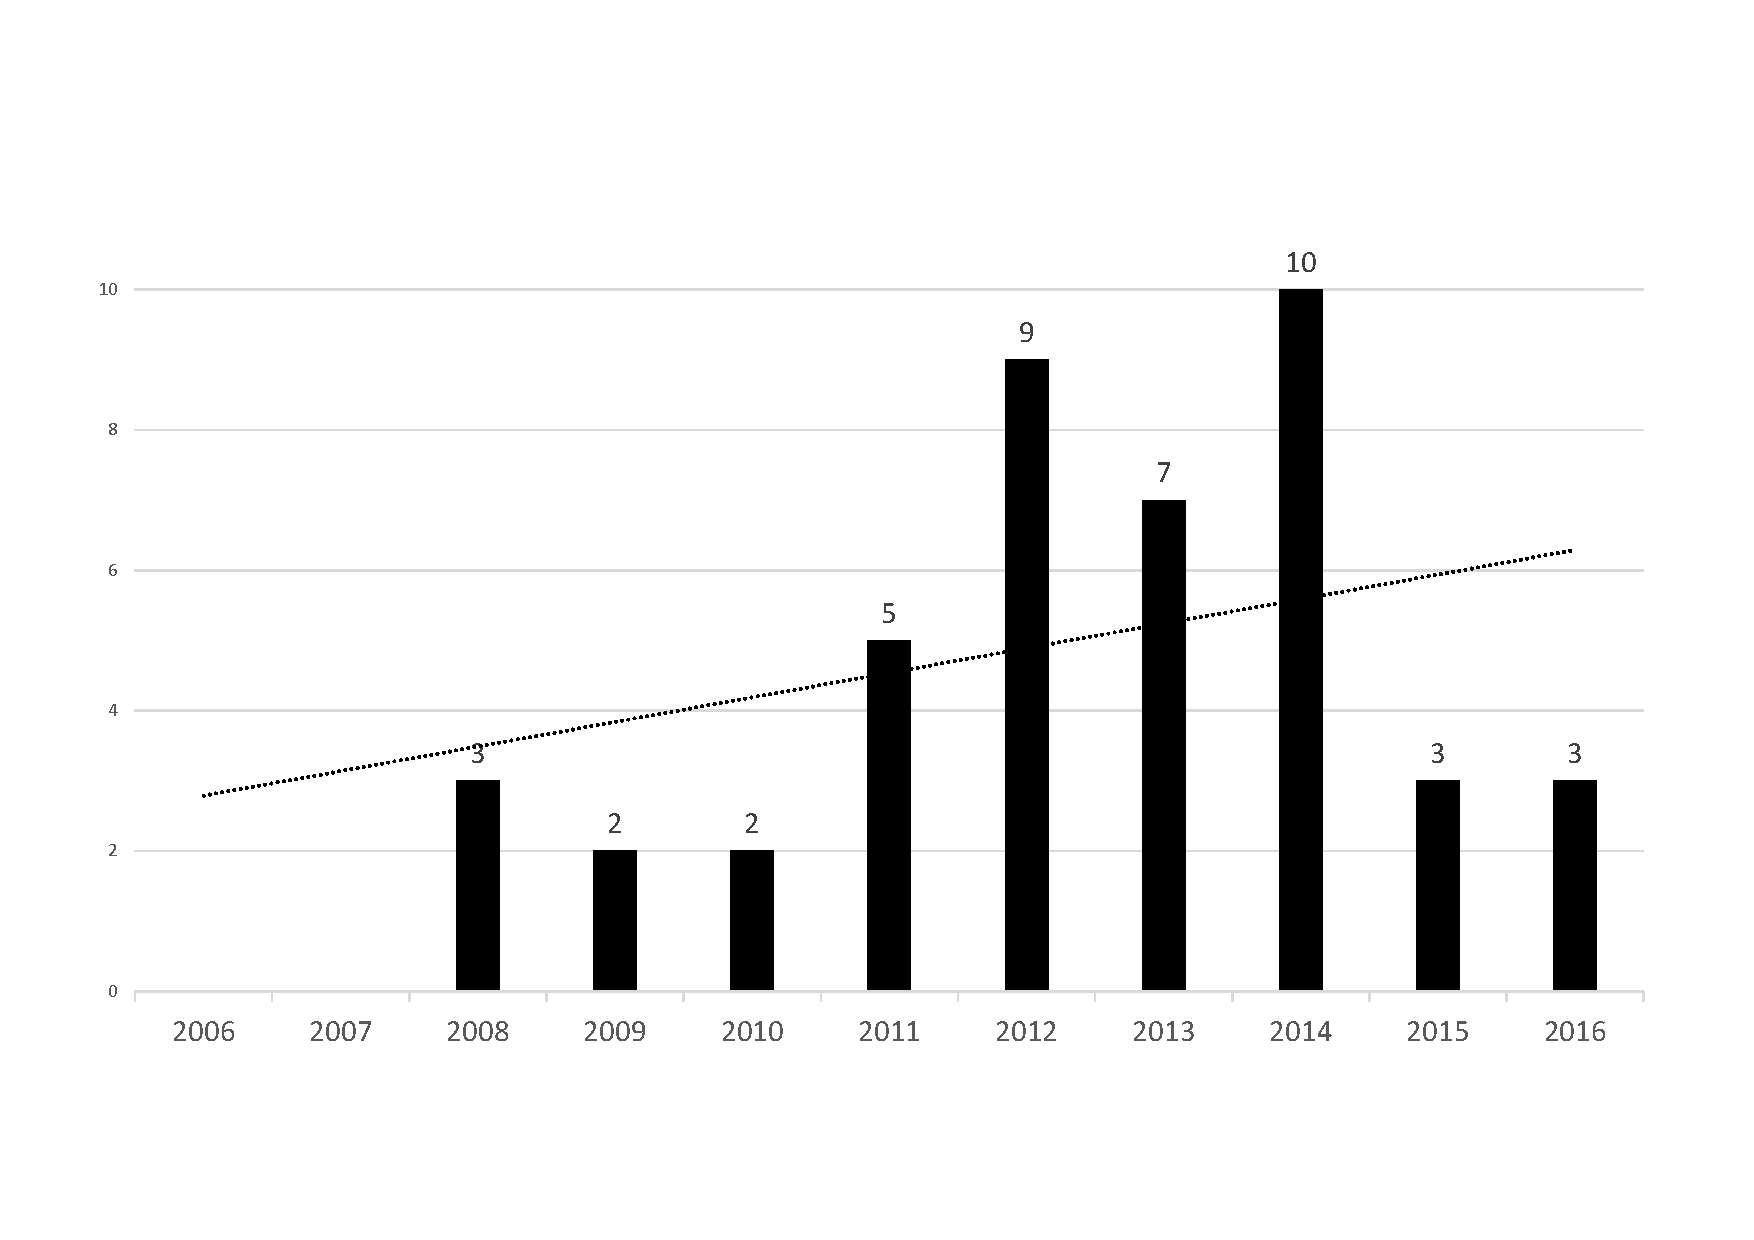
\includegraphics[scale=0.90]{quantidadeano.png}
	\label{fig:qtdano}
\end{figure}
\newpage
\section{Extração de Dados}

\subsection{Trabalhos Selecionados}

Para a extração dos dados, foram considerados 44 trabalhos restantes da 5° lista. Os atributos extraídos são os que estão contidos nas Seção \ref{sec:estrategia}. Os trabalhos utilizados para a extração se encontram na \ref{table:listaextra}

\begin{table}[]
	\centering
	\caption{Trabalhos selecionados para leitura e extração de dados}
	\label{table:listaextra}
	\resizebox{\textwidth}{!}{%
		\begin{tabular}{|c|l|l|c|c|c|c|}
			\hline
			\textbf{ID} & \multicolumn{1}{c|}{\textbf{Título}} & \multicolumn{1}{c|}{\textbf{Autor(res)}} & \textbf{Referência} & \textbf{\begin{tabular}[c]{@{}c@{}}Ano de\\ Publicação\end{tabular}} & \textbf{Fonte} & \textbf{Tipo} \\ \hline
			T1 & \begin{tabular}[c]{@{}l@{}}Delta-Oriented Model-Based SPL\\  Regression Testing\end{tabular} & \begin{tabular}[c]{@{}l@{}}Sascha Lity, Malte Lochau, \\ Ina Schaefer, Ursula Goltz\end{tabular} & \cite{lity2012delta} & 2012 & ACM & Evento \\ \hline
			T2 & \begin{tabular}[c]{@{}l@{}}Industrial Evaluation of Pairwise SPL\\ Testing with MoSo-PoLiTe\end{tabular} & \begin{tabular}[c]{@{}l@{}}Michaela Steffens, Sebastian Oster, \\ Malte Lochau, Thomas Fogdal\end{tabular} & \cite{steffens2012industrial} & 2012 & ACM & Evento \\ \hline
			T3 & \begin{tabular}[c]{@{}l@{}}Model-Based Coverage-Driven Test Suíte\\ Generation for Software Product Lines\end{tabular} & \begin{tabular}[c]{@{}l@{}}Harald Cichos, Sebastian Oster, \\ Malte Lochau, Andy Schurr\end{tabular} & \cite{cichos2011model} & 2011 & ACM & Periódico \\ \hline
			T4 & \begin{tabular}[c]{@{}l@{}}MoSo-PoLiTe - Tool Support for Pairwise\\ and Model-Based Software Product Line\\ Testing\end{tabular} & \begin{tabular}[c]{@{}l@{}}Sebastian Oster, Ivan Zorcic, \\ Florian Markert, Malte Lochau\end{tabular} & \cite{oster2011moso} & 2011 & ACM & Evento \\ \hline
			T5 & MPLM ? MaTeLo Product Line Manager & Hamza Samih, Ralf Bogusch & \cite{samih2014mplm} & 2014 & ACM & Evento \\ \hline
			T6 & \begin{tabular}[c]{@{}l@{}}On the use of test cases in model-based\\ software product line development\end{tabular} & \begin{tabular}[c]{@{}l@{}}Alexander Knapp, Markus Roggenbach, \\ Bernd-Holger Schlingloff\end{tabular} & \cite{knapp2014use} & 2014 & ACM & Evento \\ \hline
			T7 & \begin{tabular}[c]{@{}l@{}}Pairwise Feature-Interaction Testing for\\ SPLs: Potentials and Limitations\end{tabular} & \begin{tabular}[c]{@{}l@{}}Sebastian Oster, Malte Lochau, \\ Marius Zink, Mark Grechanik\end{tabular} & \cite{oster2011pairwise} & 2011 & ACM & Evento \\ \hline
			T8 & \begin{tabular}[c]{@{}l@{}}Deriving Usage Model Variants for Model-\\ based Testing: An Industrial Case Study\end{tabular} & \begin{tabular}[c]{@{}l@{}}Hamza Samih,  Hélène Le Guen, \\ Ralf Bogusch, Mathieu Acher, Benoit Baudry\end{tabular} & \cite{samih2014deriving} & 2014 & IEEE & Evento \\ \hline
			T9 & \begin{tabular}[c]{@{}l@{}}Model-based Software Product Line Testing\\ by Coupling Feature Models with\\ Hierarchical Markov Chain Usage Models\end{tabular} & Ceren Sahin Gebizli, Hasan Sozer & \cite{gebizli2016model} & 2016 & IEEE & Evento \\ \hline
			T10 & \begin{tabular}[c]{@{}l@{}}Model-Based Test Design of Product Lines:\\ Raising Test Design to the Product Line Level\end{tabular} & \begin{tabular}[c]{@{}l@{}}Hartmut Lackner, Martin Thomas, \\ Florian Wartenberg, Stephan Weißleder\end{tabular} & \cite{lackner2014model} & 2014 & IEEE & Periódico \\ \hline
			T11 & \begin{tabular}[c]{@{}l@{}}Requirements-Based Delta-Oriented SPL\\ Testing\end{tabular} & \begin{tabular}[c]{@{}l@{}}Michael Dukaczewski, Ina Schaefer, \\ Remo Lachmann, Malte Lochau\end{tabular} & \cite{dukaczewski2013requirements} & 2013 & IEEE & Evento \\ \hline
			T12 & \begin{tabular}[c]{@{}l@{}}Using Feature Model to Support Model-\\ Based Testing of Product Lines: An \\ Industrial Case Study\end{tabular} & \begin{tabular}[c]{@{}l@{}}Shuai Wang,  Shaukat Ali, \\ Tao Yue, Marius Liaaen\end{tabular} & \cite{wang2013using} & 2013 & IEEE & Periódico \\ \hline
			T13 & \begin{tabular}[c]{@{}l@{}}An automated Model-based Testing\\ Approach in Software Product Lines Using\\ a Variability Language\end{tabular} & \begin{tabular}[c]{@{}l@{}}Boni García,  Rodrigo García-Carmona, \\ Álvaro Navas, Hugo A. Parada-Gélvez, \\ Félix Cuadrado, Juan C. Dueñas\end{tabular} & \cite{garcia2010automated} & 2010 & \begin{tabular}[c]{@{}c@{}}Politécnica Arquivo \\digital UPM\end{tabular} & Evento \\ \hline
			T14 & \begin{tabular}[c]{@{}l@{}}Automated Product Line Methodologies to\\ Support Model-Based Testing\end{tabular} & Shuai Wang,  Shaukat Ali, Arnaud Gotlieb & \cite{wang2013automated} & 2013 & \begin{tabular}[c]{@{}c@{}}CEUR Evento \\ Proceedings\end{tabular} & Evento \\ \hline
			T15 & \begin{tabular}[c]{@{}l@{}}Behavioural Model Based Testing of\\ Software Product Lines\end{tabular} & Xavier Devroey & \cite{devroey2014behavioural} & 2014 & ACM & Evento \\ \hline
			T16 & Feature Model-based Software Product Line Testing & SEBASTIAN OSTER & \cite{oster2012feature} & 2012 & \begin{tabular}[c]{@{}c@{}}TUprints - TU Darmstadt \\ publication service\end{tabular} & Periódico \\ \hline
			T17 & \begin{tabular}[c]{@{}l@{}}Model-based pairwise testing for feature\\ interaction coverage in software product line\\ engineering\end{tabular} & \begin{tabular}[c]{@{}l@{}}Malte Lochau, Sebastian Oster, \\ Ursula Goltz, Andy Schurr\end{tabular} & \cite{lochau2012model} & 2011 & Springer & Periódico \\ \hline
			T18 & \begin{tabular}[c]{@{}l@{}}Model-based Test Generation for Software\\ Product Line\end{tabular} & Xinying Cai, Hongwei Zeng & \cite{cai2013model} & 2013 & IEEE & Evento \\ \hline
			T19 & \begin{tabular}[c]{@{}l@{}}Model-Based Testing for Software Product\\ Lines\end{tabular} & Erika Mir Olimpiew & \cite{olimpiew2008model} & 2008 & Springer & Evento \\ \hline
			T20 & \begin{tabular}[c]{@{}l@{}}PLETS - A PRODUCT LINE OF MODEL-\\ BASED TESTING TOOLS\end{tabular} & ELDER DE MACEDO RODRIGUES & \cite{rodrigues2013plets} & 2013 & PUC-RS & Evento \\ \hline
			T21 & \begin{tabular}[c]{@{}l@{}}Top-Down and Bottom-Up Approach for\\ Model-Based Testing of Product Lines\end{tabular} & Stephan Weißleder, Hartmut Lackner & \cite{weissleder2013top} & 2013 & EPTCS & Evento \\ \hline
			T22 & \begin{tabular}[c]{@{}l@{}}A Product Line Modeling and Configuration\\  Methodology to Support Model-Based \\ Testing: An Industrial Case Study\end{tabular} & \begin{tabular}[c]{@{}l@{}}Shaukat Ali, Tao Yue, Lionel Briand, \\ Suneth Walawege\end{tabular} & \cite{ali2012product} & 2012 & Springer & Periódico \\ \hline
			T23 & \begin{tabular}[c]{@{}l@{}}Coverage Criteria for Behavioural Testing\\  of Software Product Lines\end{tabular} & \begin{tabular}[c]{@{}l@{}}Xavier Devroey, Gilles Perrouin, \\ Axel Legay, Maxime Cordy, \\ Pierre-Yves Schobbens, Patrick Heymans\end{tabular} & \cite{devroey2014coverage} & 2014 & Springer & Evento \\ \hline
			T24 & \begin{tabular}[c]{@{}l@{}}A Model Based Testing Approach for\\  Model-Driven Development and \\ Software Product Lines\end{tabular} & \begin{tabular}[c]{@{}l@{}}Beatriz Pérez Lamancha,  Macario Polo Usaola, \\ Mario Piattini Velthius\end{tabular} & \cite{lamancha2010model} & 2010 & Springer & Evento \\ \hline
			T25 & \begin{tabular}[c]{@{}l@{}}A Vision for Behavioural Model-Driven\\  Validation of Software Product Lines\end{tabular} & \begin{tabular}[c]{@{}l@{}}Xavier Devroey, Maxime Cordy,  Gilles Perrouin, \\ Eun-Young Kang, Pierre-Yves Schobbens, Patrick Heymans,\\  Axel Legay,  Benoit Baudry\end{tabular} & \cite{devroey2012vision} & 2012 & Springer & Evento \\ \hline
			T26 & \begin{tabular}[c]{@{}l@{}}Abstract Test Case Generation for\\  Behavioural Testing of Software Product Lines\end{tabular} & \begin{tabular}[c]{@{}l@{}}Xavier Devroey, Gilles Perrouin, \\ Pierre-Yves Schobbens\end{tabular} & \cite{devroey2014abstract} & 2014 & ACM & Evento \\ \hline
			T27 & \begin{tabular}[c]{@{}l@{}}Applying Incremental Model Slicing to\\  Product-Line Regression Testing\end{tabular} & \begin{tabular}[c]{@{}l@{}}Sascha Lity, Thomas Morbach,  \\ Thomas Th¨ um, Ina Schaefer\end{tabular} & \cite{lity2016applying} & 2016 & Springer & Periódico \\ \hline
			T28 & \begin{tabular}[c]{@{}l@{}}Automated Testing of Software-as-\\ a-Service Configurations using a\\  Variability Language\end{tabular} & Sachin Patel, Vipul Shah & \cite{patel2015automated} & 2015 & ACM & Evento \\ \hline
			T29 & Delta-Oriented FSM-Based Testing & \begin{tabular}[c]{@{}l@{}}Mahsa Varshosaz,  Harsh Beohar,  \\ Mohammad Reza Mousavi\end{tabular} & \cite{varshosaz2015delta} & 2015 & Springer & Evento \\ \hline
			T30 & \begin{tabular}[c]{@{}l@{}}Incremental Model-Based Testing of \\ Delta-oriented Software Product Lines\end{tabular} & \begin{tabular}[c]{@{}l@{}}Malte Lochau, Ina Schaefer, \\ Jochen Kamischke, Sascha Lity\end{tabular} & \cite{lochau2012incremental} & 2012 & Springer & Periódico \\ \hline
			T31 & Model Based Testing in Software Product Lines & \begin{tabular}[c]{@{}l@{}}Pedro Reales, Macario Polo, \\ Danilo Caivano\end{tabular} & \cite{reales2011model} & 2011 & Springer & Evento \\ \hline
			T32 & Model-Based Testing & \begin{tabular}[c]{@{}l@{}}Malte Lochau, Sven Peldszus, \\ Matthias Kowal,  Ina Schaefer\end{tabular} & \cite{lochau2012model} & 2014 & Springer & Evento \\ \hline
			T33 & \begin{tabular}[c]{@{}l@{}}Parameterized Preorder Relations for\\  Model-Based Testing of Software Product Lines\end{tabular} & Malte Lochau, Jochen Kamischke & \cite{lochau2012parameterized} & 2012 & Springer & Evento \\ \hline
			T34 & \begin{tabular}[c]{@{}l@{}}Poster: VIBeS, Transition System\\  Mutation Made Easy,\end{tabular} & \begin{tabular}[c]{@{}l@{}}Xavier Devroey, Gilles Perrouin, \\ Pierre-Yves Schobbens, Patrick Heymans\end{tabular} & \cite{devroey2015vibes} & 2015 & IEEE & Evento \\ \hline
			T35 & Spinal Test Suites for Software Product Lines & Harsh Beohar, Mohammad Reza Mousavi & \cite{beohar2014spinal} & 2014 & EPTCS & Evento \\ \hline
			T36 & \begin{tabular}[c]{@{}l@{}}Automated model-based testing using the\\  UML testing profile and QVT\end{tabular} & \begin{tabular}[c]{@{}l@{}}Beatriz Pérez Lamancha, Pedro Reales Mateo, \\ IgnacioRodríguez de Guzmán, \\ Macario Polo Usaola, Mario Piattini Velthius\end{tabular} & \cite{lamancha2009automated} & 2009 & ACM & Evento \\ \hline
			T37 & \begin{tabular}[c]{@{}l@{}}Relating Variability Modeling and Model-\\ Based Testing for Software Product Lines\\  Testing\end{tabular} & Hamza Samih & \cite{samih2012relating} & 2012 & ICTSS & Evento \\ \hline
			T38 & \begin{tabular}[c]{@{}l@{}}An Evaluation of Model-Based Testing in\\  Embedded Applications\end{tabular} & Stephan Weißleder, Holger Schlingloff & \cite{weissleder2014evaluation} & 2014 & IEEE & Evento \\ \hline
			T39 & \begin{tabular}[c]{@{}l@{}}Assessing Software Product Line Testing\\  Via Model-Based Mutation An \\ Application to Similarity Testing\end{tabular} & \begin{tabular}[c]{@{}l@{}}Christopher Henard, Mike Papadakis, \\ Gilles Perrouin, Jacques Klein, Yves Le Traon\end{tabular} & \cite{henard2013assessing} & 2013 & IEEE & Evento \\ \hline
			T40 & \begin{tabular}[c]{@{}l@{}}Automated and Scalable T-wise Test\\  Case Generation Strategies for \\ Software Product Lines\end{tabular} & Gilles Perrouin, Sagar Sen, Jacques Klein, Benoit Baudry, Yves le Traon Lassy & \cite{perrouin2010automated} & 2010 & IEEE & Evento \\ \hline
			T41 & \begin{tabular}[c]{@{}l@{}}Model-based Testing of System\\  Requirements using UML Use Case Models\end{tabular} & Bill Hasling, Helmut Goetz, Klaus Beetz & \cite{hasling2008model} & 2008 & IEEE & Evento \\ \hline
			T42 & \begin{tabular}[c]{@{}l@{}}Successive refinement of models for\\  model-based testing to increase \\ system test effectiveness\end{tabular} & Ceren Sahin Gebizli, Hasan Sozer, Ali Ozer Ercan & \cite{gebizli2016successive} & 2016 & IEEE & Evento \\ \hline
			T43 & \begin{tabular}[c]{@{}l@{}}A Software Product Line for\\  Model-Based Testing Tools\end{tabular} & \begin{tabular}[c]{@{}l@{}}Elder M. Rodrigues, Avelino F. Zorzo, Itana M. Gimenez, \\ Elisa Y. Nakagawa, Flavio M. Oliveira, José C. Maldonado\end{tabular} & \cite{rodrigues2012software} & 2012 & PUC-RS & Outro \\ \hline
			T44 & \begin{tabular}[c]{@{}l@{}}Reusing State Machines for\\  Automatic Test Generation \\ in Product Lines\end{tabular} & Stephan Weißleder, Dehla Sokenou, Bernd-Holger Schlingloff & \cite{weissleder2008reusing} & 2008 & MoTip & Evento \\ \hline
		\end{tabular}%
	}
\end{table}


\subsection{Qualidade dos Trabalhos}
Para garantir a qualidade dos trabalhos, utilizamos a \ref{table:criterios} de critérios apresentada na Seção \ref{sec:estrategia} para auxiliar na classificação. Seguindo a tabela de questionário, aplicamos o critério aos trabalhos remanescentes para poder levantar quais teriam uma maior relação com o propósito desta RSL.

Sendo assim, originou-se a \ref{table:top10} onde encontram-se os 10 trabalhos com maior relevância e grau de importância em conteúdo, pois possuem uma grande quantidade de dados relacionados diretamente com os objetivos da RSL. Isso não significa que os que não estão listados deixam de ser significativos, somente em nível de quantidade de dados direcionados ao tema.


\begin{table}[]
	\centering
	\caption{Trabalhos com alto valor no critério de seleção}
	\label{table:top10}
	\resizebox{\textwidth}{!}{%
		\begin{tabular}{|c|l|l|c|}
			\hline
			\textbf{ID} & \multicolumn{1}{c|}{\textbf{Título}} & \multicolumn{1}{c|}{\textbf{Autores}} & \textbf{\begin{tabular}[c]{@{}c@{}}Ano de\\ Publicação\end{tabular}} \\ \hline
			T7 & \begin{tabular}[c]{@{}l@{}}Pairwise Feature-Interaction Testing for SPLs: \\ Potentials and Limitations\end{tabular} & \begin{tabular}[c]{@{}l@{}}Sebastian Oster, Malte Lochau,\\  Marius Zink, Mark Grechanik\end{tabular} & 2011 \\ \hline
			T16 & Feature Model-based Software Product Line Testing & Sebastian Oster & 2012 \\ \hline
			T19 & Model-Based Testing for Software Product Lines & Erika Mir Olimpiew & 2008 \\ \hline
			T20 & \begin{tabular}[c]{@{}l@{}}PLETS - A PRODUCT LINE OF MODEL-BASED\\ TESTING TOOLS\end{tabular} & Elder de Macedo Rodrigues & 2013 \\ \hline
			T28 & \begin{tabular}[c]{@{}l@{}}Automated Testing of Software-as-a-Service \\ Configurations using a Variability Language\end{tabular} & Sachin Patel, Vipul Shah & 2015 \\ \hline
			T31 & Model Based Testing in Software Product Lines & \begin{tabular}[c]{@{}l@{}}Pedro Reales, Macario Polo, \\ Danilo Caivano\end{tabular} & 2011 \\ \hline
			T32 & Model-Based Testing & \begin{tabular}[c]{@{}l@{}}Malte Lochau, Sven Peldszus, \\ Matthias Kowal,  Ina Schaefer\end{tabular} & 2014 \\ \hline
			T36 & Automated model-based testing using the UML testing profile and QVT & \begin{tabular}[c]{@{}l@{}}Beatriz Pérez Lamancha, Pedro Reales Mateo, \\ IgnacioRodríguez de Guzmán, Macario Polo Usaola, \\ Mario Piattini Velthius\end{tabular} & 2009 \\ \hline
			T37 & \begin{tabular}[c]{@{}l@{}}Relating Variability Modeling and Model-Based \\ Testing for Software Product Lines Testing\end{tabular} & Hamza Samih & 2012 \\ \hline
			T44 & \begin{tabular}[c]{@{}l@{}}Reusing State Machines for Automatic \\ Test Generation in Product Lines\end{tabular} & \begin{tabular}[c]{@{}l@{}}Stephan Weißleder, Dehla Sokenou, \\ Bernd-Holger Schlingloff\end{tabular} & 2008 \\ \hline
		\end{tabular}%
	}
\end{table}



\subsection{Respostas às Questões de Pesquisa}

Após a leitura dos trabalhos da \ref{table:listaextra} foi possível mapear e extrair informações para contribuir com as respostas para as questões de pesquisa desta RSL.

\subsubsection{QP1: Em quais domínios TBM tem sido aplicado em LPS?} Com relação a primeira pergunta de pesquisa, foram identificados sete domínios distintos, conforme a \ref{table:qpp1}.

O domínio software é o que contém maior incidência com 24 trabalhos, seguido do automotivo com nove, que crescentemente utiliza softwares embarcados em seus produtos.

\subsubsection{Aeroespacial}
MPLM é uma das poucas ferramentas que concentram o maior esforço na questão de solução de variabilidade na geração de casos de teste, \cite{samih2014mplm} em seu trabalho apresentam a ferramenta Matelo, em conjunto com outras ferramentas permite derivar a variante do modelo de um conjunto desejado e assim gerar casos de teste para um projeto experimental na Airbus \textit{defence \& Space}. TBM auxilia no no reaproveitamento para a geração dos casos de teste, o outro trabalho que atua no mesmo domínio é uma extensão deste citado.

\subsubsection{Automotivo}
\cite{lity2012delta} Apresenta uma abordagem delta, que trabalha com elementos transversais de um elemento denominado G, com um conjunto principal e onde os casos de testes estão definidos com cobertura satisfatória. Os artefato de teste são evoluídos de forma incremental, conforme o surgimento de novas variantes do produto. Consideramos que o fator regressão, e adaptabilidade dos artefatos de teste podem conter uma contribuição significativa por serem trabalhados em uma LPS, embora ele não tenha foco em TBM. A utilização de software embarcados nos produtos automotivos cresce exponencialmente, nesse caso levamos em consideração a variação de modelos ofertados, TBM vem auxiliando na geração dos testes destes produtos que sofrem variação, onde existe um núcleo central, e cada variação pode ou não conter uma especificidade única dos demais.

\subsubsection{Eletrônico}
Seguindo este conceito \cite{steffens2012industrial} utiliza de modelos para a geração de subgrupos ou casos de testes a partir destes modelos, aborda a questão de \textit{feature iteractio} com a cobertura de teste e gerencia as variabilidades como itens transversais. MoSo-PoLiTe, ferramenta proposta fazer a derivação dos produtos a partir do modelo principal utilizando de teste combinatório automatizado. TBM atua na geração de casos de teste para subgrupos de produtos, além de buscar garantir uma maior cobertura de erros de funcionalidade, por se tratar de um domínio eletrônico, a garantia da qualidade deve ser com uma margem significativamente maior.

\subsubsection{Manufatura}

\cite{knapp2014use} apresenta um procedimento associado a um conjunto de ferramentas para atribuir o resultado de um caso de teste a um membro arbitrário de uma LPS, usando modelos de variabilidade com base em UML e CVL, utiliza-se do modelo para a criação de máquinas de estado que em seguida são convertidas em diagrama de classe.

\subsubsection{Medicina}
\cite{hasling2008model} realiza a conversão dos modelos em diagramas de atividade e caso de uso, após essa conversão é trabalhado a criação de casos de teste, onde as variantes dos modelos podem ser considerados como variáveis. Por usar TBM, ele não menciona se a variabilidade é tratada, simplesmente utiliza para a criação de casos de teste a partir de diagramas de atividade.

\subsubsection{Software}

Software é um dos domínios mais relatados, a princípio por estar ligado diretamente ao tema da pesquisa, embora os demais domínios também utilizem TBM no processo de desenvolvimento de algum produto de software específico para aquele determinado domínio.

\cite{olimpiew2008model} também proporciona muito dados e informações sobre o TBM em LPS, embora o foco seja em diagramas de atividades customizadas, mas com um foco na reutilização do teste em produtos variantes da LPS. A abordagem proposta CADeT, transforma os casos de uso em diagramas de atividades e que por sua vez são transformados em casos de teste. As especificações de teste são rastreadas a partir do diagrama de atividade e do caso de uso.

A grande maioria dos estudos relatam a criação de alguma abordagem ou ferramenta em TBM para auxílio no desenvolvimento da LPS, no entanto, muitos não deixam bem claro alguns detalhes sobre o propósito principal da utilização de TBM sem seus trabalho. 

\subsubsection{Telecomunicação}
TBM atua no auxilio da derivação de casos de teste a partir de máquinas de estado, a atuação nesse domínio se deve a utilização de meios embarcados nos dispositivos de comunicação. Em determinado momento é possível interpretar que o trabalho referente a este domínio seria manufatura, porém ele tem uma área de atuação bem definida que seria a divisão de pesquisa de uma grande empresa de telecomunicações.

Ainda sobre a utilização de ferramentas \cite{wang2013automated} retrata a utilização de um processo automatizado de seleção de teste de forma minima e sistematizada. Processos automatizados contribuem com algoritmos de seleção, por mais que seja em uma manufatura ele ajuda a criar uma visão sistêmica de seleção de variabilidades. 

\begin{table}[]
	\centering
	\caption{Domínios de aplicação de TBM em LPS}
	\label{table:qpp1}
	\begin{tabular}{|l|l|}
		\hline
		\textbf{Domínio} & \textbf{Referência}                                                                                                                                                  \\ \hline
		Aeroespacial     & T5, T8                                                                                                                                                          \\ \hline
		Automotivo       & T1, T3, T4, T7, T10, T11, T16, T17, T30                                                                                                                              \\ \hline
		Eletrônico       & T2, T9, T42, T44                                                                                                                                                     \\ \hline
		Manufatura       & T6                                                                                                                                                                   \\ \hline
		Medicina         & T41                                                                                                                                                                  \\ \hline
		Software         & \begin{tabular}[c]{@{}l@{}}T13, T15, T18, T19, T20, T21, T23, T24, T25, T26, T27, T28,\\ T29, T31, T32, T33, T34, T35, T36, T37, T38, T39, T40, T43\end{tabular} \\ \hline
		Telecomunicação  & T12, T14, T22                                                                                                                                                        \\ \hline
	\end{tabular}
\end{table}

\subsubsection{QP2: Quais abordagens têm sido utilizadas no TBM de LPS?} Nesse ponto, todos os trabalhos da \ref{table:listaextra} utilizam a abordagem Off-line, que é o teste em tempo de modelagem.

Ainda sobre o contexto da QP2, foram considerados três itens relevantes, técnica de teste utilizada (\ref{table:tecnica}), nível de teste (\ref{table:qpp2}), e automatização de teste utilizada (\ref{table:qpp22}). 


\begin{table}[]
	\centering
	\caption{Níveis de teste aplicado aos trabalhos}
	\label{table:qpp2}
	\begin{tabular}{|l|l|}
		\hline
		\textbf{Nível de teste aplicado} & \textbf{Referência}                                                                                                    \\ \hline
		Desempenho                         & T20                                                                                                                    \\ \hline
		Estrutura                          & T20                                                                                                                    \\ \hline
		Funcionalidade                     & T9, T10, T22, T24, T28, T31, T6                                                                                        \\ \hline
		Integração                         & \begin{tabular}[c]{@{}l@{}}T3, T7, T8, T16, T19, T21, T23, T29, T37, T5, T11,\\ T13, T14,T15, T17, T18\end{tabular} \\ \hline
		Regressão                          & \begin{tabular}[c]{@{}l@{}}T11, T13, T14, T15, T17, T18, T1, T27, T30,\end{tabular}                                 \\ \hline
		Sistema                            & \begin{tabular}[c]{@{}l@{}}T25, T26, T33, T34, T35, T36, T38, T39, T40, T41,\\ T42, T43, T44\end{tabular}        \\ \hline
		Combinatório                       & T4                                                                                                                     \\ \hline
		Unidade                            & T2                                                                                                                     \\ \hline
		Não informado                       & T12, T32                                                                                                               \\ \hline
	\end{tabular}
\end{table}

\begin{table}[]
	\centering
	\caption{Automatização de teste utilizada nos trabalhos}
	\label{table:qpp22}
	\begin{tabular}{|l|l|}
		\hline
		\textbf{Abordagem de teste aplicada} & \textbf{Referência}                                                                                                                                                       \\ \hline
		Automatizada                         & \begin{tabular}[c]{@{}l@{}}T10, T11, T13, T14, T15, T16, T17, T18, T2,\\ T20, T22, T23, T24, T26, T27, T28, T3, T31,\\ T4, T40, T41, T5, T6, T7, T8, T9, T12\end{tabular} \\ \hline
		Semi Automatizada                    & \begin{tabular}[c]{@{}l@{}}T19,T21,T25,T29,T30,T34,T36,T37,T38,T39,\\ T42,T43,T44\end{tabular}                                                                        \\ \hline
		Manual                               & T1, T33, T35                                                                                                                                                              \\ \hline
		Não informado                         & T32                                                                                                                                                                       \\ \hline
	\end{tabular}
\end{table}

Sobre as técnicas utilizadas classificamos como caixa-preta quando não temos acesso ao código somente aos dados que entram e o resultado que deverá sair, já no caixa-branca temos acesso ao código fonte. Os trabalhos estão relacionados conforme a \ref{table:tecnica}.

\begin{table}[]
	\centering
	\caption{Relação de técnicas utilizadas}
	\label{table:tecnica}
	\begin{tabular}{|l|l|}
		\hline
		\textbf{Técnica de Teste} & \textbf{Referência}                                                                                                                                                                                                                                   \\ \hline
		Caixa Preta               & \begin{tabular}[c]{@{}l@{}}T2, T3, T7, T8, T9, T10, T11, T12, T13, T14, T15, T16,\\ T17, T18, T19, T21, T22, T23, T24, T25, T26, T27, T28,\\ T29, T30, T31, T32, T33, T34, T35, T36, T37, T38, T39,\\ T40, T41, T42, T43, T44\end{tabular} \\ \hline
		Caixa Branca              & T1, T4, T20                                                                                                                                                                                                                                           \\ \hline
		Não Informado             & T5, T6                                                                                                                                                                                                                                               \\ \hline
	\end{tabular}
\end{table}

Embora a maior parte dos trabalhos mencione que utiliza uma abordagem automatizada \ref{table:qpp22}, nos trabalhos não se é apresentado como isso é feito, talvez ainda por ser um conceito, ou ainda a falta da implementação da abordagem.




\subsubsection{QP3: Qual o tipo de problema em LPS que TBM tem solucionado?}
Em grande parte TBM está auxiliando na conversão do modelo em artefatos que auxiliem na identificação de possíveis problemas ou erros de interpretação. Representação do comportamento desejado, gerando a partir do caso de teste é algo que torna a cobertura dos erros satisfatória, embora a evolução das técnicas utilizadas durante o processo devem ser aprimoradas. Os modelos servem para serem convertidos, modelados, ou extraídos. Exemplo de comportamento do software.

\subsubsection{QP4: Como variabilidade é tratada no TBM de LPS?}
Na \ref{fig:variabilidade} podemos constatar que a grande maioria dos trabalhos aborda alguma forma gerenciamento de variabilidades, isso demonstra que assim como é crescente o interesse pelo tema, também existe a preocupação com a qualidade, e geral com as variações dos produtos. Na \ref{table:variabilidade} podemos observar quais trabalhos utilizam o gerenciamento de variabilidade durante o processo.

\begin{figure}[htb]
	\centering
	\caption{Proporção dos trabalhos que fazem uso de gerenciamento de variabilidade}
	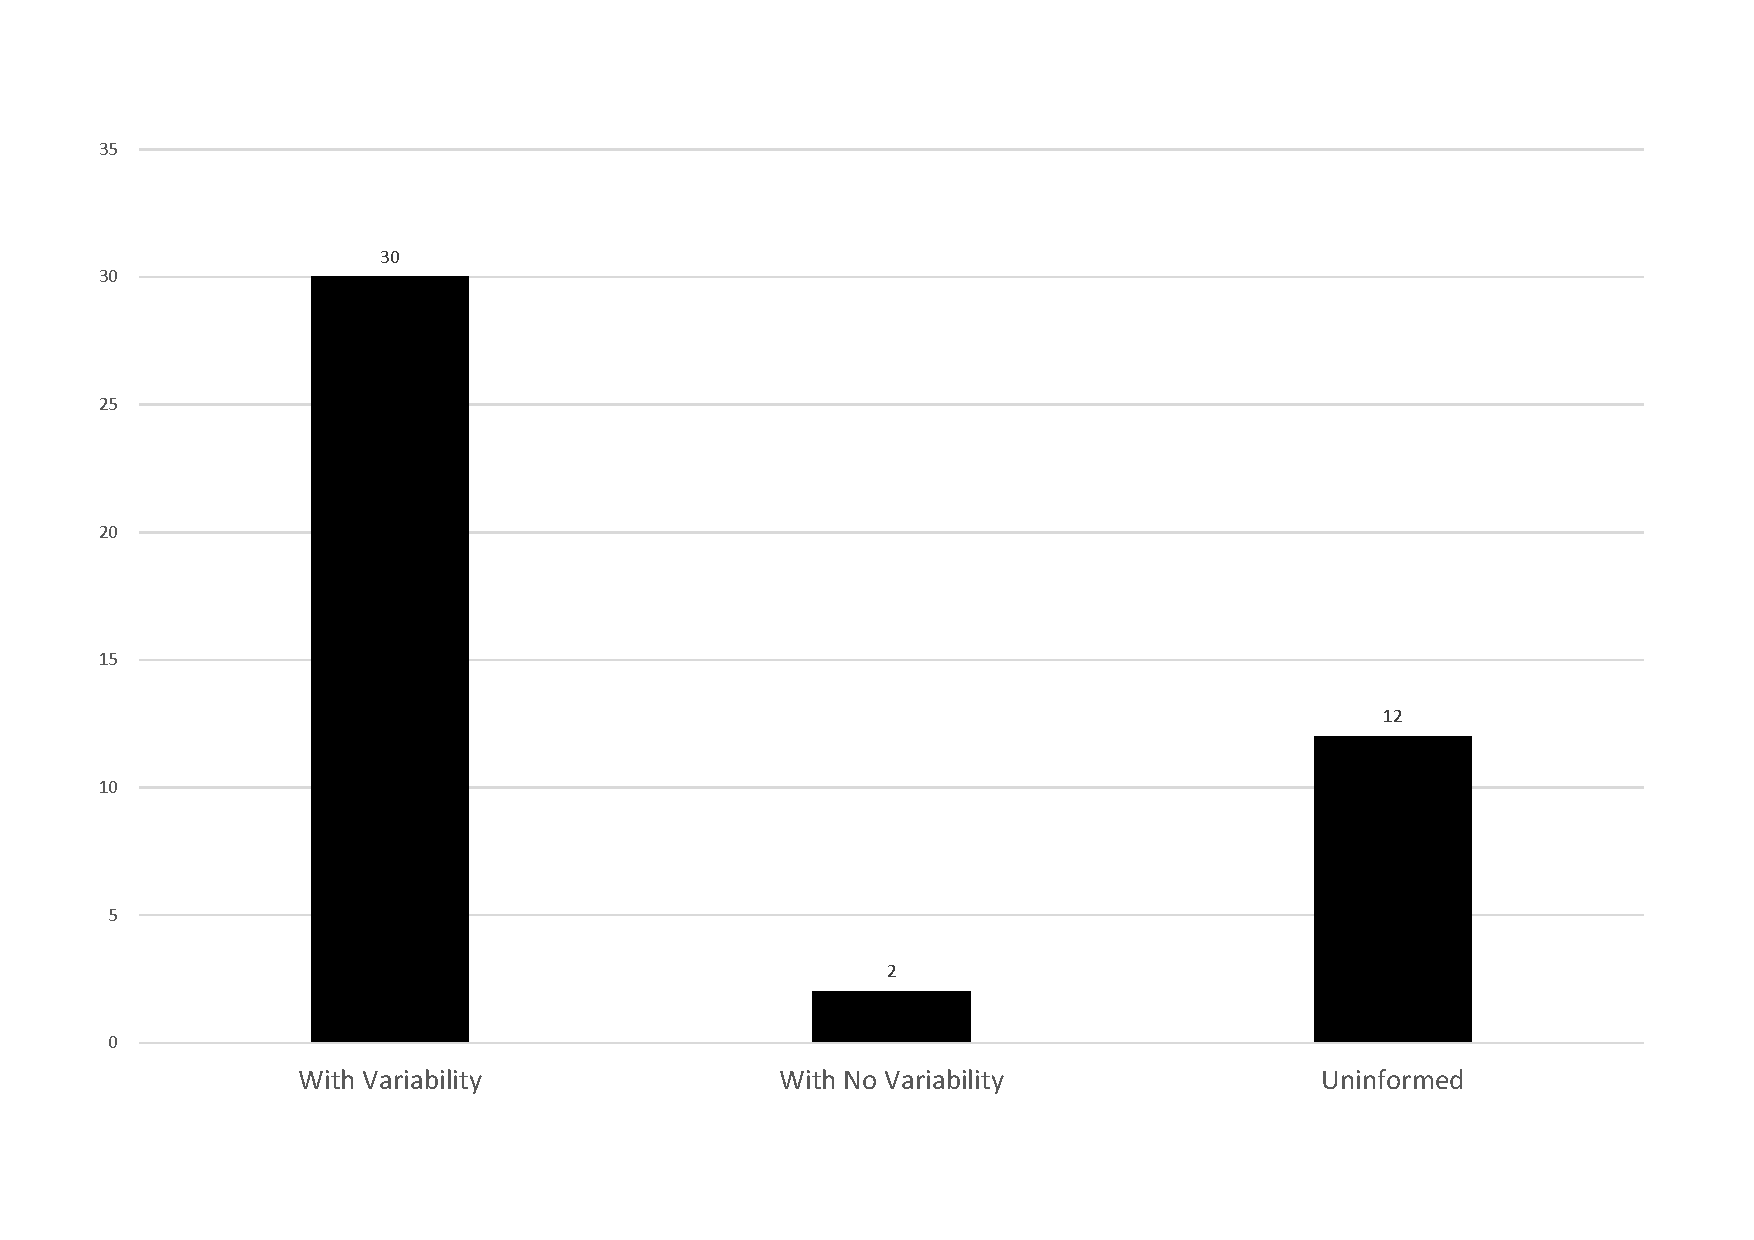
\includegraphics[scale=0.70]{variabilidade.png}
	\label{fig:variabilidade}
\end{figure}

\begin{table}[]
	\centering
	\caption{Trabalhos que consideram gerenciamento de variabilidade durante o processo de teste}
	\label{table:variabilidade}
	\begin{tabular}{|l|l|}
		\hline
		\textbf{\begin{tabular}[c]{@{}l@{}}Gerenciamento de \\ Variabilidade\end{tabular}} & \textbf{Referência} \\ \hline
		Sim & \begin{tabular}[c]{@{}l@{}}T1, T2, T4, T5, T6, T7, T8, T9, T10, T12, T13, T14, T15,\\ T16, T17, T18, T19, T21, T22, T24, T25, T27, T28, T29, \\ T30, T31, T33, T34, T37, T40\end{tabular} \\ \hline
		Não & T39, T43 \\ \hline
		Não informado & \begin{tabular}[c]{@{}l@{}}T3, T11, T20, T23, T26, T32, T35, T36, T38, T41, T42, T44\end{tabular} \\ \hline
	\end{tabular}
\end{table}


\subsubsection{QP5: Como TBM apoia o teste de requisitos não-funcionais?}
Nenhum dos trabalhos apresentados aqui nesta RSL apresenta ou menciona algum tipo de preocupação com requisitos não-funcionais, embora os produtos alvo de teste estejam em tempo de modelagem, nada impede de na criação do plano de teste incluir os requisitos não-funcionais para serem analisados ou verificados.

O ideal seria que todo plano de teste mesmo que em tempo de modelagem contemplasse partes ou a totalidade dos requisitos não-funcionais. Porém, não foram identificadas nesta RSL evidências ou itens que apoiam o teste de requisitos não-funcionais.

\newpage
\subsubsection{QP6: A geração de casos de testes utiliza artefatos ou ferramentas?}
Quando se tem o modelo e parte-se para a geração de casos de teste, muitos dos trabalhos utilizam a conversão do modelo para um determinado artefato intermediário, embora uma certa minoria realize a criação direta do modelo. Na \ref{table:artefatosutilizados} pode-se constatar quantos trabalhos utilizam um determinado artefato para a criação do caso de teste, assim como quais artefatos estão sendo utilizados.


\begin{table}[]
	\centering
	\caption{Artefatos utilizados durante o processo}
	\label{table:artefatosutilizados}
	\begin{tabular}{|l|l|}
		\hline
		\textbf{Artefato IÇntermediário} & \textbf{Referência} \\ \hline
		Máquina de Estado & \begin{tabular}[c]{@{}l@{}}T1, T6, T7, T10, T11, T12, T13, T14, T15, T17,T21,\\ T22, T23, T27, T29, T30, T34, T38, T44\end{tabular} \\ \hline
		Direto do Modelo & T8, T9, T42 \\ \hline
		\begin{tabular}[c]{@{}l@{}}Modelo de variabilidade\\ Ortogonal OVM\end{tabular} & T8 \\ \hline
		Diagrama de Classe & T6, T12, T14, T31 \\ \hline
		Diagrama de Atividade & T18, T19, T41 \\ \hline
		Caso de Uso & T20, T28, T41, T43 \\ \hline
		Diagrama de Sequência & T24, T31, T36 \\ \hline
		Diagrama de Transição & T7, T15, T25, T26, T33, T35, T37 \\ \hline
		Diagrama de Função & T9, T39, T40, T2, T3, T4, T5, T16 \\ \hline
		Não Informa & T32 \\ \hline
	\end{tabular}
\end{table}

Analisando os trabalhos e quais artefatos foram utilizados, constatou-se que muitos além de fazer a utilização de artefatos gerados a partir dos modelos, criam artefatos intermediários, que auxiliam em tomadas de decisões ou que, pela conversão direta do modelo não ser possível para o artefato desejado, se faz por meio de uma dupla conversão.


Assim como os artefatos intermediários levantamos a seguinte situação, utilização de ferramentas durante o processo, na \ref{table:ferramentas} pode ser analisado quais trabalhos fazem uso de ferramentas em qualquer parte do processo, seja para automatização, como auxilio na análise dos dados, etc.

Dentre as ferramentas citadas nos trabalhos, damos destaques as mais citadas, que foram elas: IBM RATIONAL RHAPSODY, MoSo-PoLiTe, MaTeLo Product Line Manager, SPLOT tool, PURE variantes, CADeT Tools, TRUST tool, Pralíntool, VIBeS, Eclipse, UML2 Tools entre outros.

\begin{table}[]
	\centering
	\caption{Trabalhos que fazem uso de ferramentas durante o processo}
	\label{table:ferramentas}
	\begin{tabular}{|l|l|}
		\hline
		\textbf{\begin{tabular}[c]{@{}l@{}}Faz uso de Ferramentas\\ Durante o Processo\end{tabular}} & \textbf{Referência} \\ \hline
		Sim & \begin{tabular}[c]{@{}l@{}}T1, T2, T4, T5, T6, T7, T8, T9, T10, T12, T13,\\ T14, T16, T17, T19, T22, T28, T30, T31, T34,\\ T36, T37, T38, T40, T41, T42\end{tabular} \\ \hline
		Não Informa & \begin{tabular}[c]{@{}l@{}}T3, T11, T15, T18, T20, T21, T23, T24, T25,\\ T26, T27, T29, T32, T33, T35, T39, T43, T44\end{tabular} \\ \hline
	\end{tabular}
\end{table}

\subsubsection{QP7: Quais tipos de modelos de LPS têm sido considerados no TBM?}
Quanto ao tipo de modelo de LPS considerado dentre os trabalhos analisados, a grande maioria se fez da utilização do \textit{Behavioral-based} que se caracteriza por ser comportamental, talvez o motivo seja pelo fato de os modelos serem ricos em detalhes, facilitando a interpretação ou configuração, mesmo que posteriormente o modelo seja convertido em um artefato, primário ou intermediário. Na \ref{table:cenario} pode ser observado que vários trabalhos utilizam o modelo \textit{Scenario-based models} a relação se deve ao fato de estes trabalhos fazerem a utilização de artefatos intermediários, trabalhando com cenários de utilização ao invés de comportamento direto.

\begin{table}[]
	\centering
	\caption{Modelo de LPS considerado nos trabalhos extraídos}
	\label{table:cenario}
	\begin{tabular}{|l|l|}
		\hline
		\textbf{Modelo de LPS Considerado} & \textbf{Referência} \\ \hline
		\textit{Scenario-based models} & \begin{tabular}[c]{@{}l@{}}T3,T11, T19, T20, T24, T31, T38, T40, T41,\\ T42 T43, T44\end{tabular} \\ \hline
		\textit{Class-oriented} & T6 \\ \hline
		\textit{Behavioral-based} & \begin{tabular}[c]{@{}l@{}}T1, T2, T4, T7, T8, T9, T10, T12, T13, T14,\\ T15, T16, T17, T18, T21, T22, T23, T25,\\ T26, T27, T28, T29, T30, T33, T34,T35, T36,\\ T37, T39\end{tabular} \\ \hline
		Não Informado & T5, T32 \\ \hline
	\end{tabular}
\end{table}


\subsubsection{QP8:\textit{Binding time} afeta a aplicação de TBM em LPS?}
Muitas propriedades de um programa são conhecidas durante o processo de execução ou em tempo de desenvolvimento, para isso denominamos \textit{binding time} ou tempo de resolução, neste caso, resolução da variabilidade:\textit{design-time, compile-time, linking-time, runtime}

Nesta RSL, quase que a totalidade dos trabalhos não deixa explícito o \textit{binding time}. Na \ref{table:binding} apresentamos trabalhos que baseado na interpretação dos autores desta RSL, identificaram em algum momento do texto a utilização do \textit{Design Time} como tempo de resolução de variabilidade.


\begin{table}[]
	\centering
	\caption{Estudos que indiretamente relacionam o \textit{binding time}}
	\label{table:binding}
	\begin{tabular}{|l|l|}
		\hline
		\multicolumn{1}{|c|}{\textbf{\begin{tabular}[c]{@{}c@{}}Momento de solução \\ da Variabilidade \\(Binding Time)\end{tabular}}} & \multicolumn{1}{c|}{\textbf{Referência}} \\ \hline
		Design Time & \begin{tabular}[c]{@{}l@{}}T7, T8, T9, T10, T11, T12, T13,T14, T15, T16, T17, T18,\\ T19, T20, T21, T22, T23, T24, T25, T26, T27, T28, T29,\\ T30, T31, T32, T33, T34, T35, T36, T37, T38, T39, T40,\\ T41, T42, T43, T44\end{tabular} \\ \hline
		Não Informa & T1, T2, T3, T4, T5, T6 \\ \hline
	\end{tabular}
\end{table}


\subsubsection{QP9: Como as técnicas e as atividades de TBM para LPS têm sido avaliadas?}
80\% dos trabalhos apresentados (\ref{fig:validacao} e \ref{table:coletaevidencia}) relatam qual foi o método utilizado para a avaliação das atividades. A minoria de 20\% não deixou claro ou não evidenciou se realizou algum tipo de avaliação.

\begin{figure}[htb]
	\centering
	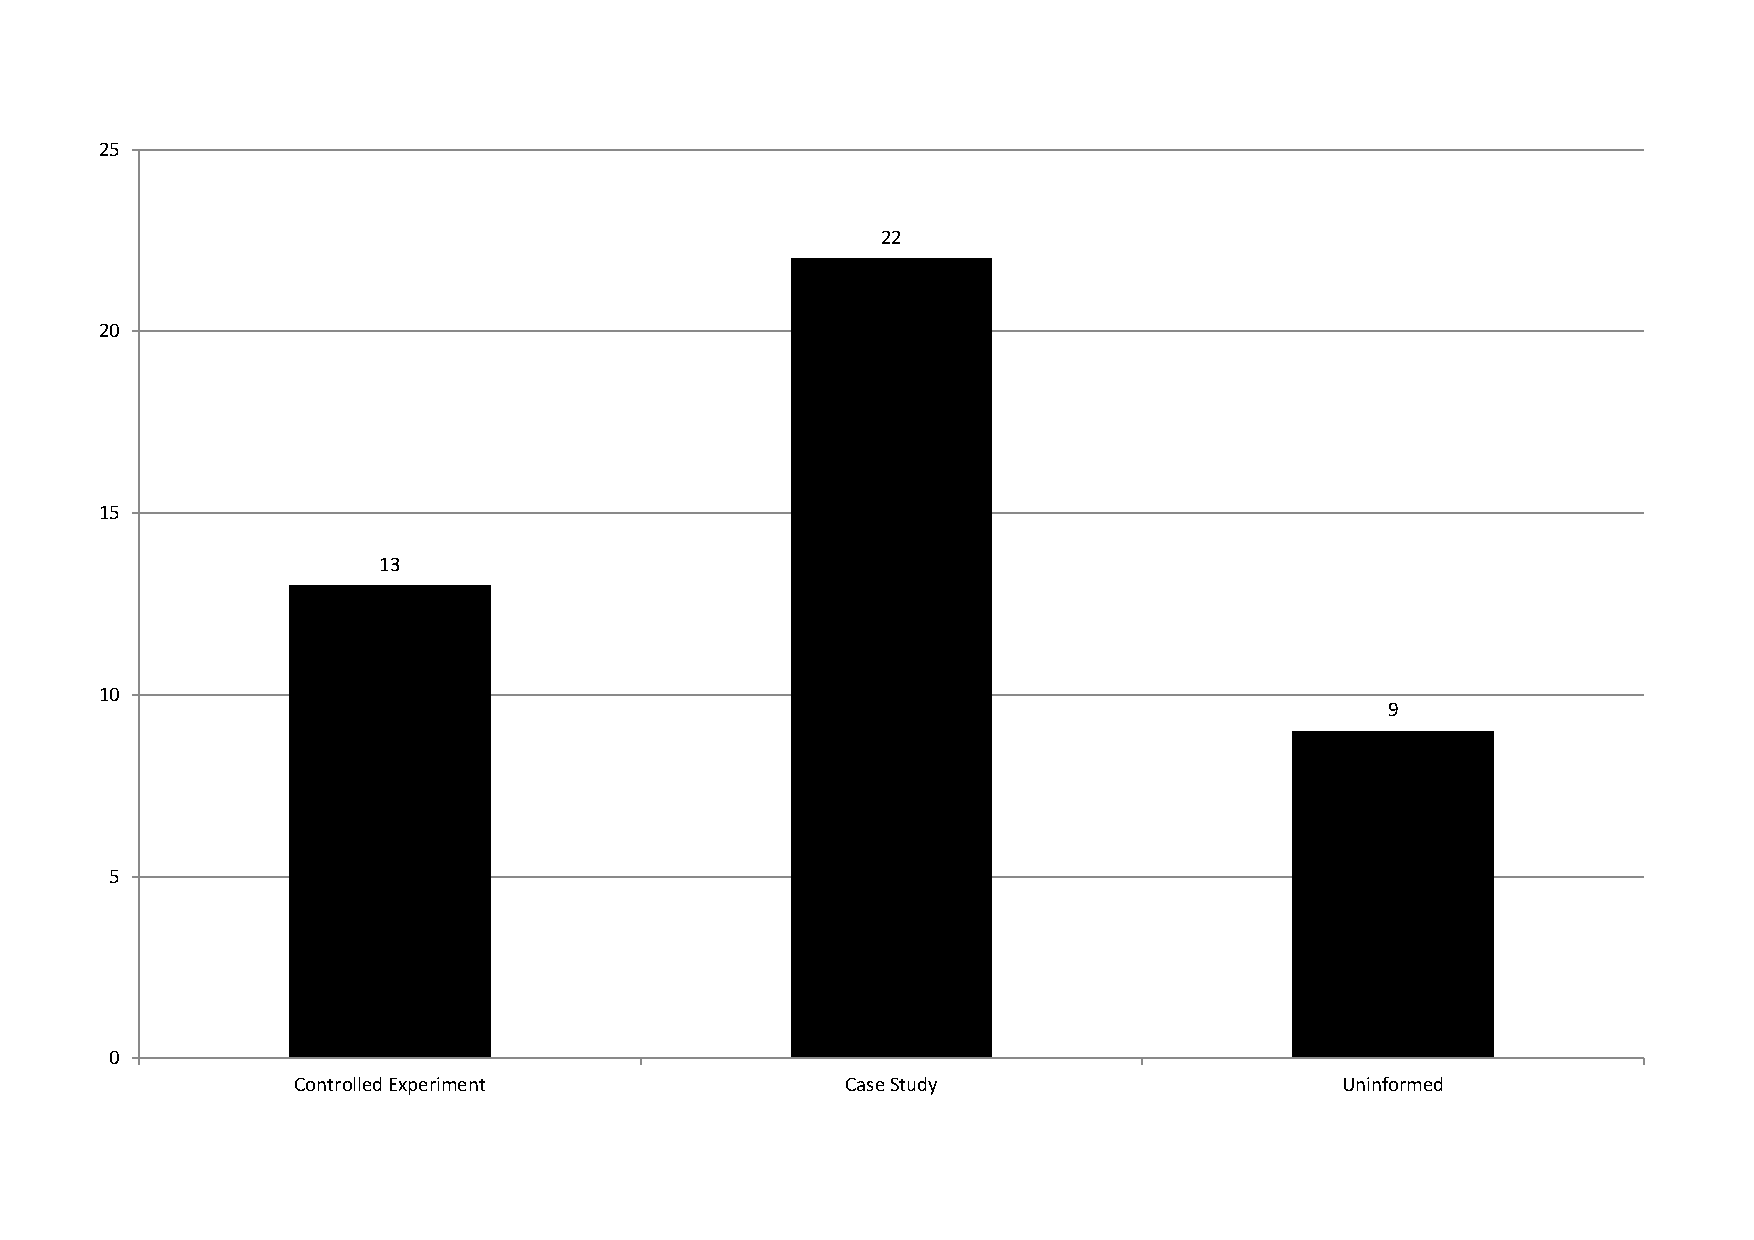
\includegraphics[scale=0.60]{validacao.png}
	\caption{Proporção dos trabalhos que validaram as atividades}
	\label{fig:validacao}
\end{figure}


\begin{table}[]
	\centering
	\caption{Relação de métodos de avaliação utilizados}
	\label{table:coletaevidencia}
	\begin{tabular}{|l|l|}
		\hline
		\textbf{\begin{tabular}[c]{@{}l@{}}Método de Coleta\\ de Evidências\end{tabular}} & \textbf{Referência} \\ \hline
		Experimento Controlado & \begin{tabular}[c]{@{}l@{}}T1, T3, T4, T16, T20, T21, T23, T24, T25, T28, T39, T40,\\ T42\end{tabular} \\ \hline
		Estudo de Caso & \begin{tabular}[c]{@{}l@{}}T2, T6, T7, T8, T9, T10, T11, T12, T13, T14, T15, T17,\\ T19, T22, T26, T27, T29, T30, T33, T38, T43, T44\end{tabular} \\ \hline
		Não evidenciado & T5, T18, T31, T32, T34, T35, T36, T37, T41 \\ \hline
	\end{tabular}
\end{table}

Isso fica evidente quando relatamos os locais de avaliação do trabalho, apresentados na tabela \ref{table:areadevalidacao}. Em análise mais aprofundada, alguns deles por mais que não evidenciem, tendem a ter utilizado estudo de caso como forma de avaliação. 

\begin{table}[]
	\centering
	\caption{Área onde foi avaliado o trabalho}
	\label{table:areadevalidacao}
	\begin{tabular}{|l|l|}
		\hline
		\textbf{\begin{tabular}[c]{@{}l@{}}Área \end{tabular}} & \textbf{Referência} \\ \hline
		Indústria & \begin{tabular}[c]{@{}l@{}}T1, T2, T3, T4, T5, T6, T7, T8, T9, T10, T11, T12, T13,\\ T14, T15, T16, T17, T20, T22, T29, T30, T38, T41, T42,\\ T43, T44\end{tabular} \\ \hline
		Academia & \begin{tabular}[c]{@{}l@{}}T19, T23, T24, T25, T26, T27, T28, T31, T32, T33, T34,\\ T35, T36, T37, T39, T40\end{tabular} \\ \hline
		Não evidenciado & T18, T21 \\ \hline
	\end{tabular}
\end{table}

\newpage
\subsubsection{QP10: É realizado a rastreabilidade em TBM para LPS?}
Ao final da análise dos trabalhos, procuramos encontrar quais foram as principais contribuições apresentadas. Quando falamos em qualidade uma das principais contribuições que esperamos é que sejas contemplados todos ou a maioria do fatores que proporcione qualidade ao produto gerado, além das técnicas, níveis e tipos de testes um ponto que deve ser levado em consideração é o rastreamento das atividades durante o processo.

Ele garante que qualquer alteração que seja realizada possa ser verificada sua origem e alterações, neste quesito podemos conferir na \ref{table:rastreabilidade} quais trabalhos fazem utilização de rastreabilidade, o que gera certa preocupação é que neste ponto, a grande maioria não menciona ou não faz utilização, o que pode gerar inconsistências ou retrabalho. 
\begin{table}[]
	\centering
	\caption{Trabalhos que abordam a utilização de rastreabilidade}
	\label{table:rastreabilidade}
	\begin{tabular}{|l|l|}
		\hline
		\textbf{\begin{tabular}[c]{@{}l@{}}Faz uso de \\ Rastreabilidade\end{tabular}} & \textbf{Referência} \\ \hline
		Sim & T5, T7, T15, T16, T17, T19, T20, T24, T31, T36, T37, T41, \\ \hline
		\begin{tabular}[c]{@{}l@{}}Não faz \\ ou não menciona\end{tabular} & \begin{tabular}[c]{@{}l@{}}T1, T2, T3, T4, T6, T8, T9, T10, T11, T12, T13, T14, T18, T21,\\ T22, T23, T25, T26, T27, T28, T29, T30, T32, T33, T34, T35,\\ T38, T39, T40, T42, T43, T44\end{tabular} \\ \hline
	\end{tabular}
\end{table}

\subsubsection{QP11: Soluções propostas para TBM? }
Além da rastreabilidade, levantamos quais a principais contribuições que os trabalhos apresentam e que pode ser conferido na \ref{table:contribuicao}, podemos constatar que a grande maioria dos trabalhos apresenta como contribuição uma abordagem de utilização ou de processo. Isso demonstra que existe um interesse pela contribuição com novas práticas TBM para LPS.

\begin{table}[]
	\centering
	\caption{Principais contribuições dos trabalhos relacionados}
	\label{table:contribuicao}
	\begin{tabular}{|l|l|}
		\hline
		\textbf{\begin{tabular}[c]{@{}l@{}}Principais Contribuições\\ dos Trabalhos\end{tabular}} & \textbf{Referência} \\ \hline
		Abordagem & \begin{tabular}[c]{@{}l@{}}T1, T5, T6, T7, T8, T9, T10, T11, T13, T14, T15, T16,\\ T17, T18, T20, T21, T22, T23, T24, T27, T28, T29,\\ T30, T31, T35, T36, T37, T38, T39, T41, T42, T43, T44\end{tabular} \\ \hline
		Algoritmo & T3, T25, T26 \\ \hline
		Conjunto de ferramentas & T40 \\ \hline
		Estratégia & T33 \\ \hline
		Extensão de Abordagem & T12 \\ \hline
		Ferramenta & T2, T4, T34 \\ \hline
		Metodologia & T19 \\ \hline
		Tutorial & T32 \\ \hline
	\end{tabular}
\end{table}


\newpage
\section{Discussão Geral}
Esta Seção apresenta um mapeamento de várias questões de pesquisa respondidas nesta RSL com relação aos estudos e as fases do processo de TBM. Três fases consideram, artefato, gerenciamento e verificação e execução da TBM.

\begin{landscape}
	
	\begin{figure}[htb]
		\centering
		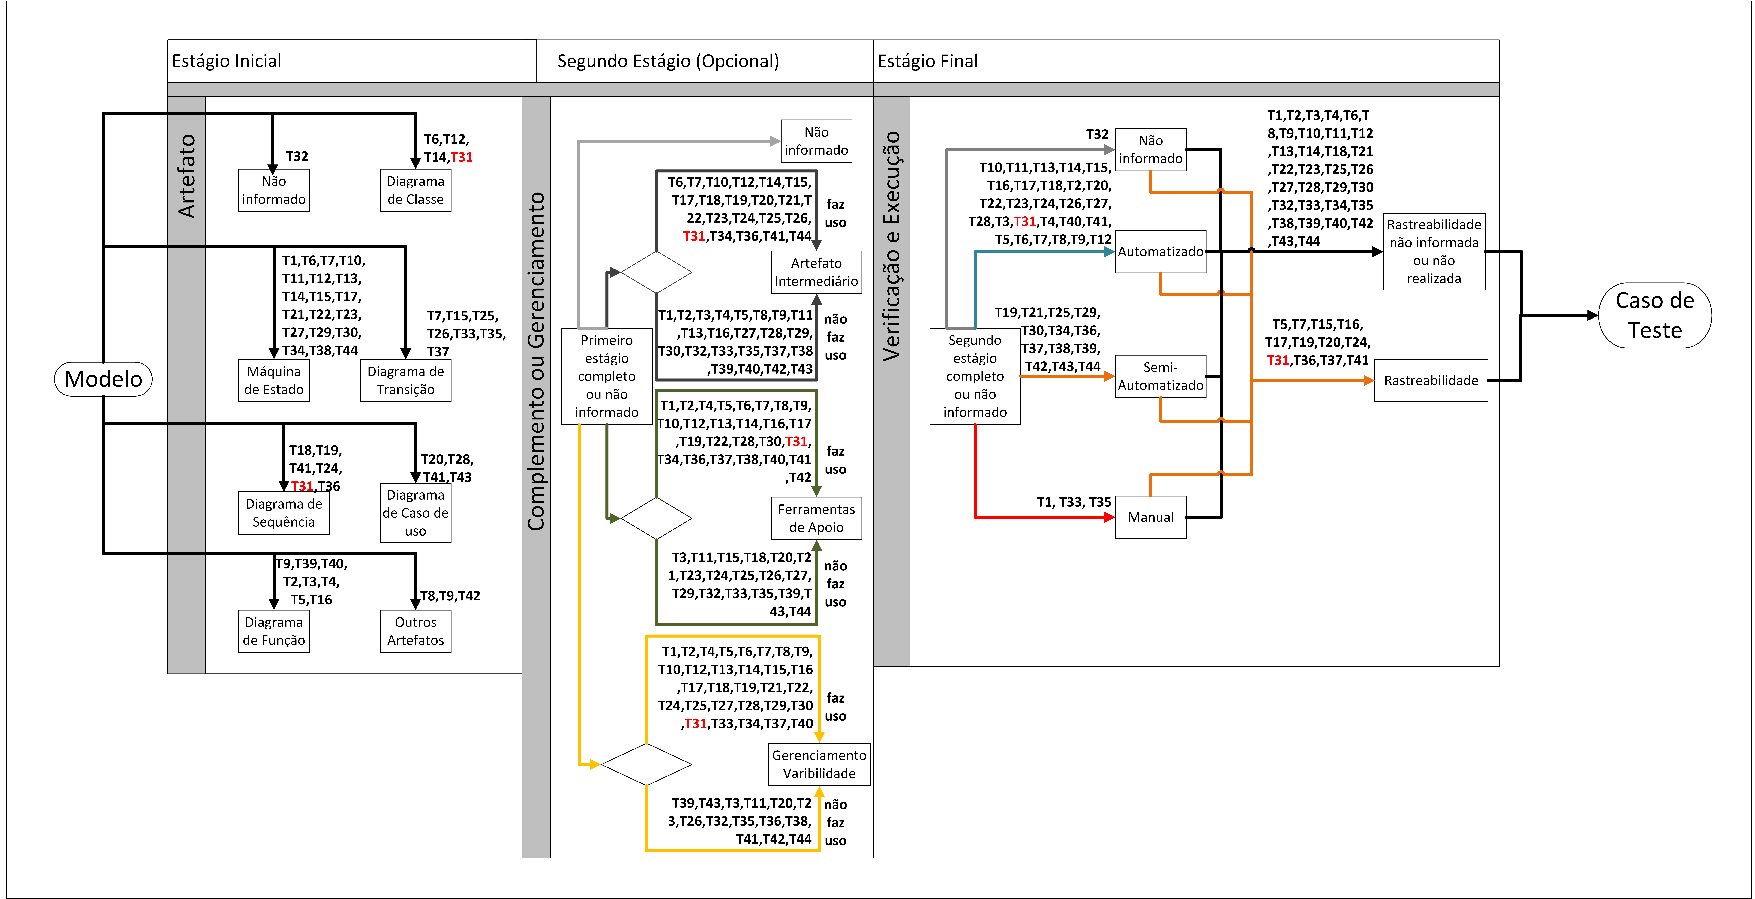
\includegraphics[scale=0.40]{guiaestudo.png}
		\caption{Guia de direcionamento de processo de TBM em LPS}
		\label{fig:guiaestudo1}
	\end{figure}
	
\end{landscape}

Porém, antes temos que explicar alguns conceitos a respeito do guia, para facilitar a busca ou compreensão dele. Após, iremos abordar os principais estudos relacionados e suas contribuições.

A \ref{fig:guiaestudo} apresenta um guia de como os estudos estão divididos de acordo com as fases e atividades de TBM. Para ilustrar o guia serão apresentados dois cenários: o primeiro em que se deseja saber o ciclo completo, a partir de um modelo até a geração de casos de teste, e suas etapas para um determinado trabalho; e o segundo cenário, em que a busca se dá pelo tema e não pelo trabalho, o que permite saber quais trabalhos, por exemplo, fazem uso de ferramentas de apoio, ao TBM.

\subsubsection{Cenário 1 - Percurso por Trabalho}

Digamos que ao selecionar um trabalho da \ref{table:listaextra} a partir de sua ID deseja-se verificar no guia da \ref{fig:guiaestudo} qual caminho ele percorre identificando os seus estágios e as suas atividades. Sendo assim, inicialmente analisarmos o primeiro estágio representado na \ref{fig:estagio1}, que é um excerto da \ref{fig:guiaestudo}.

\begin{figure}[htb]
	\centering
	\includegraphics[scale=0.80]{estagio1.png}
	\caption{Estágio Inicial do processo de TBM em LPS}
	\label{fig:estagio1}
\end{figure}
Pega-se, por exemplo, o trabalho T31. A partir de um modelo, T31 faz uma conversão para o artefato diagrama de sequência, assim podemos considerar o T31. Com o estágio inicial concluído, o segundo estágio (opcional) é então iniciado e T31 considera gerenciamento de variabilidade, apoio de ferramentas, e geração de artefatos intermediários, visto que neste estágio abordamos gerenciamento de variabilidade, uso de ferramentas, geração de artefatos intermediários e caso ele não realize nenhuma dessas atividades automaticamente ele poderia estar na geração de caso de teste.


\begin{figure}[htb]
	\centering
	\includegraphics[scale=0.80]{estagio2.png}
	\caption{Segundo estágio do processo de TBM em LPS}
	\label{fig:estagio2}
\end{figure}

\begin{figure}[htb]
	\centering
	\includegraphics[scale=0.80]{estagio3.png}
	\caption{Estágio final do processo de TBM em LPS}
	\label{fig:estagio3}
\end{figure}

Apresentando o estágio final na \ref{fig:estagio3} pode-se analisar que o trabalho T31 faz uso de processo automatizado e utiliza rastreabilidade durante o processo. Assim, completa-se o percurso do para para o trabalho T31 e assim identificar por quais etapas o trabalho reportou.

\subsubsection{Cenário 2 - Percurso por Tema}
O segundo cenário realiza o percurso por tema da TBM em LPS por assunto. Analisando a \ref{fig:estagio3}, por exemplo, pode-se verificar quais os trabalhos que fazem o uso de rastreabilidade. Portanto, se o interesse do leitor for por trabalhos que fazem o uso de rastreabilidade basta simplesmente remeter-se à essa atividade para se obter a lista de tais trabalhos.



\subsubsection{Estudos Secundários}
Para garantir a qualidade e confiança das informações relatadas neste trabalho, realizamos uma busca por estudos secundários sobre o tema. 
\cite{isa2017model} apresenta uma RSL sobre TBM para LPS, porém, consideramos que por ter deixado de seguir alguns padrões recomendados por \cite{kitchenham2004procedures}, ele apresenta inúmeras ameaças a validade além de não poder ser replicado. 

No estudo ele cita que indica modelos e estratégias utilizados, porém não apresenta dados e nem indicadores de quais estudos levantados apresenta tais itens. A quantidade de trabalhos reportados pela \textit{string} de busca está muito abaixo do reportado por esta RSL, devido a baixa cobertura de palavras chave.

Relata que cobre os problemas que foram resolvidos utilizando TBM, mas apresenta dois ou três tipos que já vem sendo reportados em teste em LPS, não agrega quais soluções estão sendo utilizadas. Além de outros fatores não reportados como, variabilidade, tipos de modelos formais utilizados, uso de ferramentas de apoio, geração de casos de teste entre outros. Por isso achamos necessário a realização deste estudo secundário, devido a grande quantidade de informações não reportadas.

\subsubsection{Trabalhos Relacionados}
Dos 44 trabalhos restantes, procuramos delinear um caminho de informações que ampliassem a visão sobre TBM em LPS com foco em variabilidade, assim, o objetivo desta seção é apresentar os fatos principais de cada trabalho referente ao objetivo da RS.

\cite{lity2012delta} Apresenta uma abordagem delta, que trabalha com elementos transversais de um elemento denominado G, com um conjunto principal e onde os casos de testes estão definidos com cobertura satisfatória. Os artefato de teste são evoluídos de forma incremental, conforme o surgimento de novas variantes do produto. Consideramos que o fator regressão, e adaptabilidade dos artefatos de teste podem conter uma contribuição significativa por serem trabalhados em uma LPS, embora ele não tenha foco em TBM.

Seguindo este conceito \cite{steffens2012industrial} utiliza de modelos para a geração de subgrupos ou casos de testes a partir destes modelos, aborda a questão de \textit{feature iteractio} com a cobertura de teste e gerencia as variabilidades como itens transversais. MoSo-PoLiTe, ferramenta proposta fazer a derivação dos produtos a partir do modelo principal utilizando de teste combinatório automatizado.

\cite{cichos2011model} aborda a questão dos conflitos da engenharia com os padrões ISO 26262 onde exige que cada configuração critica de segurança tenha bem definido os critérios de cobertura, assim ele buscar abordar este dilema apresentando um conjunto de teste com base em algoritmo de geração que usa técnicas de teste baseada em modelos, com isto eles pretendem fazer a geração completa de testes para a LPS. Isso se torna interessante no ponto de vista de que teste exaustivo é inviável, talvez com a implementação de um algoritmo fazendo o trabalho de combinação pode ser que esse viés seja contornado.

\cite{oster2011moso} traz um estudo prévio ao \cite{steffens2012industrial} que apresenta a ferramente MoSo-PoLiTe, voltado para a geração de \textit{scripts} de teste a partir de modelos, se os mesmo princípios apresentados por \cite{steffens2012industrial}, o que agrega é o detalhamento de como o processo automatizado é realizado.

MPLM é uma das poucas ferramentas que concentram o maior esforço na questão de solução de variabilidade na geração de casos de teste, \cite{samih2014mplm} em seu trabalho apresentam a ferramenta Matelo, em conjunto com outras ferramentas permite derivar a variante do modelo de um conjunto desejado e assim gerar casos de teste para cada variante.
Ainda que ele utilize modelos ortogonais, contribui muito para o TBM em LPS principalmente no quesito gerenciamento de variabilidade.

\cite{knapp2014use} apresenta um procedimento associado a um conjunto de ferramentas para atribuir o resultado de um caso de teste a um membro arbitrário de uma LPS usando modelos de variabilidade com base em UML e CVL, soma mais uma visão sobre como realizar o gerenciamento de variabilidades em uma LPS conforme a variação do produto.

Nesta fase podemos observar que a grande maioria dos estudos utilizam-se de artefatos de máquinas de estado, \cite{oster2011pairwise} trabalha com a conversão do modelo em máquina de estado, ele aborda que as características de \textit{feature interaction} são uma base para um modelo de falha, pois são reveladas normalmente durante a execução e troca de informações. 

O critério é cobrir quantas interações entre diferentes recursos possíveis, aumentando assim a probabilidade de encontrar erros, neste caso eles propõem uma abordagem combinatória de recursos para a realização de uma cobertura abrangente, no caso uma maior cobertura de interações de recursos é alcançada em uma fração custo menor. A contribuição para nosso trabalho seria o sistema de mapeamento de \textit{feature} assim como a combinação das interações para análise de cobertura, podemos considerar que ele aborda os principais pontos desta pesquisa, onde ele utiliza ferramentas, faz o gerenciamento das variabilidades, além de prover a rastreabilidade durante o processo.

\cite{samih2014deriving} é um complemento do trabalho de \cite{samih2014mplm} abordagem que adota TBM, ela esta integrada a ferramenta apresentada por \cite{samih2014mplm}.

Pensando em uma abordagem para a reutilização sistemática dos modelos para se testar uma grande família de produtos, \cite{gebizli2016model} se fizeram utilizar da cadeia hierárquica de Markov esses modelos captura todos os possíveis cenários de uso para uma família de sistemas, assim como documentar a variabilidade explicitamente e separadamente com um recurso modelo.

\cite{lackner2014model} buscam a geração de casos de teste no nível da LPS, no caso eles estão atuando em um domínio automotivo, mas podemos extrair algumas técnicas visando a questão de conversão do modelo e a verificação da variação do produto, que não fica atrelado ao item principal.

Quando abordamos variabilidade, um do maiores problemas é a reutilização do mesmo caso de teste quando existe uma variável do produto, seguindo a mesma linha de \cite{lity2012delta}, \cite{dukaczewski2013requirements} aborda a modelagem delta para utilização em LPS menos formal. Eles apresentam dados relacionados ao alto índice de reuso em contraste com o baixo numero de reteste, se os casos não forem totalmente compatíveis.

\cite{wang2013using} aborda que no contexto de TBM em LPS o esforço para desenvolver modelos pode ser significativamente reduzido caso seja utilizado uma metodologia de modelagem e configuração sistemática, para isso apresentam uma metodologia que captura a variabilidade em máquina de estado UML e gera os casos de testes a partir destes artefatos e com a ajuda de uma ferramenta gera os testes executáveis. A contribuição esperada é a forma como os processos podem ser automatizados na geração dos casos de teste.

\cite{garcia2010automated} Apresenta uma abordagem de teste automatizado para LPS, utilizando máquina de estado e modelo de variabilidade, o teste baseado em modelo fornece uma técnica para automação e geração de casos de teste usando modelos UML, trabalho importante contextualizando o método utilizando ferramentas como \textit{JUnit Test Suite} onde é apresentado todo o processo de automatização.

Ainda sobre a utilização de ferramentas \cite{wang2013automated} retrata a utilização de um processo automatizado de seleção de teste de forma minima e sistematizada. Processos automatizados contribuem com algoritmos de seleção, por mais que seja em uma manufatura ele ajuda a criar uma visão sistêmica de seleção de variabilidades. 

Essa visão sistêmica pode ser visualizada também em \cite{devroey2014behavioural} onde utiliza uma linguagem de especificação de variabilidades TVL, e utiliza os modelos para criação de \textit{statecharts} para identificação das variabilidades, a partir deles criar os cenários para testes.

Assim como \cite{oster2012feature} que faz das mesmas atribuições durante o processo, apresenta um trabalho com um conteúdo de \textit{background} muito rico de informações sobre variabilidade e reuso em LPS, além dos principais pontos de teste em LPS. Apresenta também uma proposta de teste combinatório bem extensa, onde não utiliza conversão do modelo para a geração dos casos de teste.

A contribuição do trabalho esta relacionado diretamente a quantidade de dados e informações relacionadas, os principais elementos necessários para a criação de uma visão macro sobre teste, variabilidade, modelos em LPS, além de apresentar uma gama de ferramentas que foram utilizadas durante o processo.

\cite{lochau2012model} faz continuidade do estudo de \cite{oster2011pairwise} adicionando uma definição concisa de dependências de recursos e interações de características do ponto de vista do teste, e discutem os critérios de adequação para a cobertura paralela em SPL, apresentam testes de interação e dão uma generalização ao caso T-wise.

Seguindo a geração de casos de teste a partir da SPL, \cite{cai2013model} trazem uma abordagem baseada em modelo para testar geração de casos de testes para SPLs, onde possa ser reutilizável esses cenários de teste e de domínio que são gerados a partir de diagramas de atividades estendido com pontos de variação e, em seguida, teste dos cenários de acordo com os pontos de variação.

\cite{olimpiew2008model} também proporciona muito dados e informações sobre o TBM em LPS, embora o foco seja em diagramas de atividades customizadas, mas com um foco na reutilização do teste em produtos variantes da LPS. A abordagem proposta CADeT, transforma os casos de uso em diagramas de atividades e que por sua vez são transformados em casos de teste. As especificações de teste são rastreadas a partir do diagrama de atividade e do caso de uso.

A contribuição seria relacionada ao processo de reutilização de caso de teste conforme a mudança de característica do produto, pois segundo a abordagem, pode ser usado para criar especificações de teste reutilizáveis para cobrir todos cenários de casos de uso.

Trabalhando a partir de casos de uso \cite{rodrigues2013plets}, a ferramenta PLETS procura trabalhar uma LPS de ferramentas de teste que tenham suporte a TBM e um ambiente automatizado para apoiar a geração dessas ferramentas. Podemos considerar que as contribuições para o trabalho é o meio modelo do processo de geração de \textit{scripts} de teste, que foi comparado com uma ferramente \textit{Capture and replay} e obteve um desempenho melhor.

Compartilhando um visão \textit{top down} \cite{weissleder2013top} utiliza os modelos em conjunto com a modelagem de recursos e comportamento em uma visão \textit{top down} para a geração de diagramas de estado e comportamento, contribuem para uma visão macro da modelagem como um todo e os processos bem definidos. Algo interessante realizado neste estudo é que modelagem de recursos e design de teste baseado em modelo, essa combinação no entanto, raramente foi o foco da investigação.

Máquinas de estado são também utilizadas por \cite{ali2012product} onde os modelos são convertidos, e através deles é que se faz a verificação de variabilidade.

\cite{devroey2014coverage}Utiliza de uma estrutura matemática para representar o comportamento de uma forma concisa onde os modelos utilizados para a extração de máquinas de estado e a partir dai a geração de casos de teste. Não deixa explicito o gerenciamento de variabilidade, mas ele utiliza do critério de combinação para controlar as possíveis variações de funções existentes.

Já \cite{lamancha2010model} utiliza o modelo de variabilidade Ortogonal OVM, já os modelos são convertidos em modelos de design e a partir deles são gerados os modelos de teste.

\cite{devroey2012vision} realiza a utilização do modelo para a criação de um padrão de QA, composto por 3 etapas, modelagem, \textit{design} e validação. A partir do modelo é gerado o comportamento esperado e assim criado os diagramas de transições entre os estados, assim, a variabilidade é tratada durante a geração dos diagramas de máquinas de estado, quando gerado os casos de testes é verificado sua abrangência de cobertura.

\cite{devroey2014abstract} faz a utilização de algoritmo matemático para a classificação dos modelos conforme critérios pré definidos pelo usuário, assim os modelos serão utilizado para a criação de máquinas de estados e a partir disso realizar a derivação de casos de testes a partir do comportamento destes modelos.Não menciona se faz o gerenciamento de variabilidade, devido a geração de casos de teste ser automatizada por algoritmo, então ele busca gerar todos os casos de testes possíveis baseado no critério de cobertura especificado pelo engenheiro de teste.

Utilizando-se do modelo para verificação do comportamento entre os mesmos quando ocorrido alterações,\cite{lity2016applying} faz uma análise dos casos de testes gerados, para assim a geração de novos casos de testes serem condizentes e para utilização em casos de reteste.
As variabilidades são tratadas através de modelagem orientada a Delta, onde é criado um núcleo comum e as variantes são tratadas como variantes deste núcleo, tem se um núcleo comum e adaptações do mesmo para os demais artefatos.

A Criação de um modelo base para poder obter uma análise de variabilidades, após realizar a geração de scripts de teste conforme a especificação da variabilidade, é o que propõe \cite{patel2015automated}. Tratar as variabilidades a partir de um modelo padrão que é criado para extração de casos de teste.

\cite{varshosaz2015delta} faz a utilização dos modelos para conversão em diagramas de estado finito, já na modelagem delta é trabalhado um modelo núcleo que a partir dele se derivam as funcionalidades, trabalho similar ao de \cite{lity2016applying} e \cite{lochau2012incremental}, embora a variabilidade seja tratada de forma que um núcleo comum é criado e as variações geradas a partir deste núcleo comum é que são tratadas como variabilidade.

\cite{reales2011model},\cite{lochau2012parameterized}, \cite{lamancha2009automated} e \cite{samih2012relating} Trabalham diretamente dos modelos e são exclusivamente utilizados para a geração dos diagramas necessários para a criação dos casos de teste, e no quesito de variabilidade é modelado utilizando notação ortogonal OVM.
Já \cite{weissleder2014evaluation} trabalha a partir do modelo mas não faz uso de OVM.

\cite{lochau2012model}Utiliza o modelo como uma abordagem formal para o teste funcional dinâmico, basear todas as atividades de teste em um modelo de teste formal do comportamento esperado.
Menciona que existe um controle sobre as variabilidades, mas não explica de qual forma isso é feito, relata que existem técnicas de gestão de variabilidades que são trabalhadas em conjunto com a abordagem, mas não menciona quais.

\cite{devroey2015vibes} trabalha com os modelos convertidos em máquinas de estados finito para a verificação das variáveis. Através de um quadro onde é analisado a mutação e apresentado todas as variabilidades existente em um único modelo.

Modelo convertido em sistema de transição é então analisado todas as possíveis variáveis, porém \cite{beohar2014spinal} não menciona se é feito alguma modelagem, só aborda que os testes criados são trabalhados como uma coluna vertebral onde os novos recursos são testados e agregados a esse volume central.

Faz uso para a criação de modelos similares com erros incluídos de forma proposital afim de garantir que a técnica de teste seja eficaz, \cite{henard2013assessing} não aborda o ponto de variabilidade, visa somente a derivação de modelos para os testes.

Os modelos são derivados em submodelos e para em seguida serem utilizados para a geração de casos de testes, e por utilizar uma gama de ferramentas as variabilidades são tratadas na geração dos casos de teste onde os modelos originados em submodelos dos modelos principais segundo \cite{perrouin2010automated}

\cite{hasling2008model} realiza a conversão dos modelos em diagramas de atividade e caso de uso, após essa conversão é trabalhado a criação de casos de teste, onde as variantes dos modelos podem ser considerados como variáveis, mas não relata como e onde esse ponto é tratado durante o processo. De forma similar \cite{gebizli2016successive} trabalha o modelo refinando até se chegar aos processos de transições, mas não menciona se é tratada a variabilidade ou como seria tratado, o foco fica somente nos modelos.

\cite{rodrigues2012software}Utiliza a arquitetura de referência que suporta MBT em LPS, não modela a variabilidade, ficando a cargo de um plugin de terceiro por este trabalho. Ao contrário de \cite{weissleder2008reusing} que apresenta um novo método de utilização do modelo em formato de máquina de estado onde variabilidade é expressada por pré ou pós condições ou valores de atributos de classe correspondente.



\section{Ameaças à Validade}
0As seguintes ameaças à validade deste estudo são discutidas:

\begin{itemize}
	\item Questão de Pesquisa: o objetivo desta RSL foi encontrar estudos publicados que abordam TBM em LPS. De acordo com essa condição, onze questões de pesquisa com abrangência ao objetivo foram definidas para este estudo. assim, outras questões importantes podem ter ficado de fora deste estudo e, portanto, assuntos pertinentes à esta revisão podem não ter sido abordados.
	\item Viés de Publicação: não é possível garantir que todos os estudos primários relacionados com o tema deste estudo secundário foram encontrados. Esse problema pode ocorrer porque os motores de busca não são tão precisos como se deseja para o processamento e execução de consultas de acordo com as palavras-chaves definidas.
	\item O protocolo desta RSL foi revisado por outros pesquisadores, e isso pode diminuir as ameaças a este estudo.	

	
\end{itemize}


\section{Considerações Finais}
Após a análise dos dados extraídos da RSL realizada, foi possível constatar e identificar quais as técnicas de teste TBM utilizadas, e quais utilizam notação UML, os trabalhos que realizam um controle de variabilidade, assim como a rastreabilidade. Também como são gerados os casos de testes, de forma manual ou automatizada.

As contribuições para o TBM em LPS são ricas em detalhes quanto os artefatos utilizados, as técnicas reportadas, utilização de ferramentas e uso do gerenciamento de variabilidades, são os principais dados que esta RSL contribui de maneira geral.

Em resumo, existe um crescente interesse pelo tema, embora não podemos identificar o porque da rastreabilidade e os teste de requisitos não funcionais, não estarem explicitamente apresentados, estudos mais aprofundados sobre essas duas temáticas poderão dizer mais a respeito.

Um dos pontos principais que é o gerenciamento de variabilidade atrelado ao modelo em LPS, foi apresentado por uma maioria significativa, isso demonstra que existe uma crescente consciência relacionado qualidade do produtos variantes originados de um produto principal.



\chapter{Teste Baseado em Modelos para LPS: um Mapeamento Sistemático da Literatura}
\label{sec:secmsl_MSL}
\pagestyle{plain}

\section{Planejamento do MSL}
\label{sec:secmsl_planejamentosml}
\subsection{Objetivo da Pesquisa}
O objetivo deste mapeamento sistemático da literatura é identificar estudos sobre Teste Baseado em Modelo (TBM) para Linha de Produto de Software (LPS) com foco em variabilidade, domínio de aplicação, ferramenta, modelos de LPS, entre outros.

A MSL apresentada aqui segue padrões definidos como principais orientações para a execução de um mapeamento sistemático da literatura por \citet{kitchenham2004procedures} e \citet{keele2007guidelines}.

\section{Metodologia de Pesquisa}
\label{sec:sec_mslmetodologia}

Elaboramos a metodologia de pesquisa seguindo as diretrizes de \citet{petersen2015guidelines} e \citet{kitchenham2015evidence}.

A \ref{fig:mapping_process} mostra a visão geral do nosso processo de mapeamento sistemático.

\begin{figure} [!h]
	\centering
	\includegraphics[scale=0.50]{sm_process.pdf}
	\caption{Visão geral do processo de mapeamento sistemático}
	\label{fig:mapping_process}
\end{figure}

Começamos nosso estudo definindo questões de pesquisa (Seção \ref{sec:secmsl_objetivos_equestao}). Em seguida, realizamos o processo de pesquisa (Seção \ref{sec:search_process}) para reunir um conjunto inicial de estudos primários de várias fontes diferentes. Com este conjunto de estudos, realizamos o processo de seleção (Seção \ref{sec:selection_process}), filtrando estudos de acordo com diferentes critérios. O processo de extração (Seção \ref{sec:extraction_process}) foi realizado nos estudos filtrados para suportar o processo de análise. Não processo de análise (Seção \ref{sec:analysis_process}) respondemos as questões de pesquisa definidas para este estudo.


\subsection{Objetivo e Questões de Pesquisa}
\label{sec:secmsl_objetivos_equestao}

Este MSL \textbf{tem como objetivo} coletar evidências da literatura, \textbf{com o propósito de} caracterizar Testes Baseados em Modelo, \textbf{com relação a} sua aplicação em Linhas de Produto de Software, \textbf{do ponto de vista de} Pesquisadores de LPS, \textbf{no contexto de} diferentes fontes digitais de estudo primário.

Nós formulamos seis questões de pesquisa com base no objetivo principal deste MSL, como segue:

\begin{itemize}
	
	\item \textbf{RQ.1: Para quais domínios do aplicativo LPS, tipos de solução e propostas o TBM é usado?}% 1 + 3 + 11
	Estamos interessados em reunir evidências de quais domínios de LPS são mais frequentes, como, por exemplo, software, aeroespacial e automotivo, bem como que tipo de soluções foram propostas para TBM de LPSs;
	
	\item \textbf{RQ.2: Quais abordagens de TBM, níveis de teste e artefatos foram usados para testar LPSs?} Nesta questão, o foco principal é identificar técnicas de TBM, níveis de teste e automação de teste;
	
	\item \textbf{RQ.3: Como a variabilidade e o tempo de ligação são tratados durante o TBM das LPSs?}% 4 + 8
	Nesta questão, gostaríamos de compreender quais estudos primários levam em conta a variabilidade e como eles realizam o gerenciamento da variabilidade nas atividades de TBM da LPS, bem como se o tempo de ligação afeta as atividades do TBM nas LPSs;
	
	\item \textbf{RQ.4: O TBM suporta testes de requisitos não-funcionais de LPS?} Estamos interessados em coletar evidências se os estudos primários dependem do teste de requisitos não-funcionais de LPS;
	
	\item \textbf{RQ.5: Como as propostas de TBM de LPS são avaliadas?} As soluções de TBMs de LPSs devem ser avaliadas como um meio de fornecer evidência de sua viabilidade. Portanto, gostaríamos de entender que tipo de avaliação é realizada, como experimentos controlados e estudos de caso;
	
	\item \textbf{RQ.6: Como a rastreabilidade é considerada durante atividades de TBM para LPSs?} Rastreabilidade é um conceito fundamental de TBM e LPS. Nesta questão, reunimos evidências de como as soluções consideram tal conceito para atividades de TBM em LPS.
	
\end{itemize}

\subsection{Processo de Pesquisa}
\label{sec:search_process}

A \ref{fig:search_process} mostra o processo de busca do MSL.

\begin{figure} [!h]
	\centering
	\includegraphics[scale=0.55]{search_process.pdf}
	\caption{Processo de pesquisa por MSL}
	\label{fig:search_process}
\end{figure}

A estratégia de busca para encontrar estudos primários relevantes definidos para este MSL é baseada principalmente na seleção de termos e sinônimos relacionados ao TBM aplicado ao LPS. Esses termos e sinônimos levam em consideração algumas das palavras-chave de trabalhos relacionados e são apresentadas da seguinte forma:

\begin{itemize}
	\item \textbf{\textit{software}};
	\item \textbf{\textit{product line}}:\textit{product-line}, \textit{product family}, \textit{product-family}, \textit{product-families}, \textit{family of products};
	\item \textbf{\textit{model-based testing}}:\textit{model based testing}, \textit{TBM}.
\end{itemize}

Uma vez que tivemos esses termos e seus sinônimos, associamos esses sinônimos ao operador lógico `` OR '' e termos com `` AND ''. Assim, criamos nossa \textit{string} de pesquisa geral, conforme apresentado na \ref{tab:search_string}.

\begin{table}[!h]	
	\centering
	\caption{String de pesquisa geral do MSL}
	\label{tab:search_string}
	\begin{tabular}{@{}c@{}}	
		\hline			
		software \textbf{AND} (``product line'' \textbf{OR} ``product-line'' \textbf{OR} \\``product family'' \textbf{OR} ``product-family'' \textbf{OR} ``product-families'' \textbf{OR} \\``family of products'' \textbf{OR} variability) \textbf{AND} (``model-based testing'' \textbf{OR} \\``model based testing'' \textbf{OR} TBM)	
		\\\hline
	\end{tabular}
\end{table}

Além disso, selecionamos fontes de pesquisa (eletrônica e manual), idioma dos estudos primários e tipo de publicação da seguinte forma:

\begin{itemize}
	\item \textbf{Fontes de Pesquisa:} bases de dados eletrônicas indexadas (IEEE, ACM, ScienceDirect, Scopus, Biblioteca TET IET, Google Scholar, Springer) listadas na \ref{table:fontes} e pesquisa manual em revistas especializadas, conferências e workshops como na \ref{table:conferences} e \ref{table:journals};
	
	\item \textbf{Linguagem de Estudos:} Inglês, devido à sua abrangência na área de Ciência da Computação;
	
	\item \textbf{Tipo de Publicação:} estudos primários revisados por pares publicados em periódicos, conferências / workshops ou capítulos de livros.
\end{itemize}

As razões para escolher essas fontes de pesquisa estão listadas:

\begin{itemize}
	\item fonte de ciência da computação mundialmente conhecida;
	\item fornece um mecanismo de pesquisa avançado capaz de lidar com consultas avançadas;
	\item indexado internacionalmente;
	\item índices de origem conferências e periódicos mais relevantes em Engenharia de Software;
	\item índices de fontes de artigos com fator de alto impacto (JCR e / ou índice H);
	\item Fonte não cessou a publicação.
\end{itemize}

\begin{table}[!h]
	\centering
	\scriptsize
	\caption{Fontes de pesquisa eletrônicas definidas}
	\label{table:fontes}
	\begin{tabular}{l|l}
		\hline \hline
		\textbf{Fonte Eletrônica} & \textbf{URL}                               							\\\hline
		ACM Digital Library  & \url{http://dl.acm.org}                                         \\\hline
		IEEE Xplore          & \url{http://ieeexplore.ieee.org}                                \\\hline
		ScienceDirect        & \url{http://www.sciencedirect.com}                              \\\hline
		Scopus               & \url{http://www.info.sciverse.com/scopus}                       \\\hline
		Springer             & \url{http://www.springer.com}                                   \\\hline
		Google Scholar       & \url{https://scholar.google.com}                                 \\\hline
		IET  Digital Library & \url{http://digital-library.theiet.org/content/journals/iet-sen} \\\hline
		\hline
	\end{tabular}
\end{table}

\begin{table}[!h]
	\centering
	\scriptsize
	\caption{Conferências Definidas e Workshops para Pesquisa Manual}
	\label{table:conferences}
	\begin{tabular}{l|l}
		\hline \hline
		\textbf{Acrônimo} & \textbf{Conferência/Workshop}                                 \\\hline
		ICECCS         & Engineering of Complex Computer Systems                        \\\hline
		AISE           & Advanced Information Systems Engineering                       \\\hline
		ICST           & International Conference on Software Testing                   \\\hline
		ICIS           & Computer and Information Science                               \\\hline
		ACM SIGSOFT    & Software Engineering Nãotes                                     \\\hline
		MSIS           & Workshop on Variability Modeling of Software-Intensive Systems \\\hline
		ILPS           & International Software Product Line Conference                 \\\hline
		ICSTSS         & International Conference on Testing Software and Systems       \\\hline
		QA\&TEST       & International Conference on Software QA and Testing            \\\hline
		IFIP           & International Conference on Testing Software and Systems       \\\hline
		\hline
	\end{tabular}
\end{table}

\begin{table}[!h]
	\centering
	\scriptsize
	\caption{Diários Definidos para Pesquisa Manual}
	\label{table:journals}
	\begin{tabular}{l|l}
		\hline \hline
		\textbf{Acrônimo} & \textbf{\textit{Journal}}                    \\\hline
		STVR					 & Software Testing, Verification \& Reliability \\\hline
		ESE            & Empirical Software Engineering      \\\hline
		JSS            & Journal of Systems and Software     \\\hline
		IST            & Information and Software Technology \\\hline
		ASC            & Applied Soft Computing              \\\hline
		SQJ            & Software Quality Journal            \\\hline
		SCP            & Science of Computer Programming     \\\hline
		\hline
	\end{tabular}
\end{table}

Como última atividade do processo de busca, realizamos a busca por estudos primários aplicando a string de busca a fontes eletrônicas, e buscando estudos primários manualmente em congressos, workshops e periódicos, conforme apresentado nas próximas seções. Um total de 271 estudos (Lista \# 1) foram recuperados no final deste processo.

\subsubsection{Avaliação de protocolo}

Elaboramos um questionário \footnote{\url{https://drive.google.com/open?id=1U0zfLS6JLfO6krrFkbpwL0mflCtrNkVBJ5cGKDjWfJw}} para avaliar nosso protocolo MSL para coletar a opinião de pesquisadores que trabalharam com TBM e / ou LPS, para facilitar a construção da pesquisa. O questionário é composto por oito itens, sete questões em escala de Likert \cite{li2013novel} e uma questão aberta, como segue:

\begin{enumerate}
	\item Este estudo baseia-se em uma importante questão de pesquisa em \textit{Model-Based Testing} (TBM) de linhas de produto de software (LPS).
	\item A cadeia de pesquisa é adequadamente derivada das questões de pesquisa.
	\item As fontes de pesquisa definidas são suficientes para cobrir estudos relevantes.
	\item Os critérios de inclusão e exclusão são adequados e adequadamente descritos.
	\item A pesquisa pode avaliar a qualidade / validade dos estudos selecionados.
	\item O processo de extração aborda adequadamente as questões de pesquisa.
	\item O processo de análise é apropriado para responder às questões de pesquisa.
\end{enumerate}

Cada pergunta do tipo likert tem as seguintes opções como respostas:

\begin{itemize}
	\item \textbf{Eu discordo totalmente:} quando o protocolo não atende aos critérios da pergunta de forma alguma;
	\item \textbf{Discordo Parcialmente} quando o protocolo não atende a alguns critérios da questão;
	\item \textbf{Neutro:} quando o protocolo não deixa claro se ele atende ou não aos critérios da questão;
	\item \textbf{Eu Concordo Parcialmente} quando o protocolo atende a alguns critérios da questão; e
	\item \textbf{Eu concordo plenamente:} quando o protocolo atende totalmente aos critérios da pergunta.
\end{itemize}

para os pesquisadores anotarem onde quer que julguem importante sobre o protocolo

Na parte inferior do questionário, uma opção foi disponibilizada para sugestões gratuitas sobre melhorias do protocolo. O objetivo principal desta avaliação foi refinar o protocolo com base nas respostas e sugestões dos pesquisadores.

Enviamos o questionário de avaliação para sete pesquisadores na área de Sistemas de Informação, Engenharia de Software e Engenharia Elétrica (ver \ref{table:avaliadores}). Disponibilizamos o questionário por 20 dias. Nós tivemos cinco respostas.

\begin{table}[!h]
	\centering
	\scriptsize
	\caption{Pesquisadores que avaliaram o protocolo de MSL}
	\label{table:avaliadores}
	\begin{tabular}{c|c|l|l}
		\hline \hline
		\textbf{ID} & \multicolumn{1}{c|}{\textbf{\begin{tabular}[c]{@{}c@{}}Nível de educação\end{tabular}}} & \multicolumn{1}{c|}{\textbf{Instituição}} & \multicolumn{1}{c}{\textbf{Área Especialista}} \\\hline
		R.1 & Ph.D. & Universidade Federal de Tecnologia do Paraná					& Sistemas de informação \\\hline
		R.2 & Ph.D. & Universidade Federal do Pampa											& Engenharia de software \\\hline
		R.3 & Ph.D. & Universidad Politècnica de València Espanha 		& Engenharia elétrica \\\hline
		R.4 & Ph.D. & Universidade Federal do Paraná										& Engenharia de software \\\hline
		R.5 & M.Sc. & Instituto SENAI de Tecnologia em Metalmecânica 			& Engenharia elétrica \\\hline
		\hline
	\end{tabular}
\end{table}

Os pesquisadores convidados fizeram uma avaliação muito produtiva. Todos consideram que a pesquisa pode gerar dados satisfatórios com base no contexto apresentado sobre o tema. A maioria também concorda que o Search String é adequado com base nas questões de pesquisa.

Outro ponto de concordância é que as fontes e os tipos de pesquisa podem abranger estudos relevantes, mas com relação aos critérios de inclusão e exclusão, alguns discordaram, por exemplo, que a seleção de artigos está limitada a apenas os últimos 10 anos de pesquisa. Nesse caso, a justificativa seria evitar o estudo duplicado que foi atualizado ou continuado.

Uma sugestão foi realizar uma avaliação baseada no número de citações de um determinado estudo. Essa sugestão foi aplicada em conjunto com o questionário de critérios.

\subsubsection{Busca Eletrônica}
\label{sec:searchelectronic}

Realizamos a busca eletrônica de agosto / 2017 a outubro / 2017. Nós derivamos nossa \textit{string} de busca geral para cada uma das fontes eletrônicas, como apresentado em \ref{tab:string_sources}.

\begin{table}[ht]
	\centering
	\scriptsize
	\caption{Fontes eletrônicas e sequências de pesquisa adaptadas}
	\label{tab:string_sources}
	\begin{tabularx}{\columnwidth}{c|X} 
		\hline \hline
		\textbf{\begin{tabular}[c]{@{}c@{}}Fonte Eletrônica\end{tabular}} & \multicolumn{1}{c}{\textbf{String de pesquisa adaptada}} \\\hline \hline
		
		ACM &  (\textit{``software" +``product line'' ``product-line'' ``product family'' ``product-family'' ``product-families''	``family of products'' ``variability" +``model-based testing'' ``model based testing'' ``TBM"}) \\\hline
		
		Google Scholar &  (\textit{``Software'') AND (``product line'' or ``product-line'' or ``product family'' or ``product-family'' or ``product-families'' or ``family of products'' or ``variability'') AND (``model-based testing'' or ``model based testing'' or ``TBM''}) \\\hline
		
		IEEE &  (\textit{(``software'') AND (``product line'' OR ``product-line'' OR ``product family'' OR ``product-family'' OR ``product-families'' OR ``family of products'' OR ``variability'') AND (``model-based testing'' OR ``model based testing'' OR ``TBM'')}) \\\hline
		
		Springer &  (\textit{(software)  AND  (''product line'' or ''product-line'' or ''product family'' or ''product-family'' or ''product-families'' or ''family of products'' or ''variability'')  AND  (''model-based testing'' or ''model based testing'' or TBM)} \\\hline
		
		Scopus & \textit{(TITLE-ABS-KEY ( software )  AND  TITLE-ABS-KEY ({product line}  OR {product-line}  OR {product family}  OR {product-family}  OR {product-families}  OR {family of products}  OR {variability} )  AND  TITLE-ABS-KEY ({model-based testing}  OR {model based testing}  OR {TBM} ) )  AND  ( PUBYEAR  $>$  2005 ) } \\\hline
		
		Science Direct & \textit{(``software'') AND (``product line'' OR ``product-line'' OR ``product family'' OR ``product-family'' OR ``product-families'' OR ``family of products'' OR ``variability'') AND (``model-based testing'' OR ``model based testing'' OR ``TBM'')} \\\hline
		
		IET Digital Library & \textit{((``software'') AND (``product line'' OR ``product-line'' OR ``product family'' OR ``product-family'' OR ``product-families'' OR ``family of products'' OR ``variability'') AND (``model-based testing'' OR ``model based testing'' OR ``TBM''))} \\\hline			
		\hline 
	\end{tabularx}	
\end{table}

A busca eletrônica retornou 251 estudos, como podemos ver na \ref{table:buscaauto}, coluna `` Retornado ''. A Science Direct foi a fonte mais voltada, com 125 estudos, seguida pela Scopus, com 62 estudos.

\begin{table}[!h]
	\centering
	\scriptsize
	\caption{Número de estudos de fontes eletrônicas}
	\label{table:buscaauto}	
	\begin{tabular}{l|c|c|c|c}
		\hline \hline
		\multicolumn{1}{c|}{\textbf{Fonte Eletrônica}} & \textbf{Retornou} & \textbf{Aceitos} & \textbf{Duplicados} & \textbf{Rejeitados} \\\hline \hline
		Science Direct 																	& 125 							& 07 								& 00 									& 118 \\\hline
		Scopus 																					& 62 								& 10 								& 21 									& 31 \\\hline
		IEEE Xplore 																		& 25 								& 00 								& 00 									& 25 \\\hline
		ACM 																						& 20 								& 16 								& 01 									& 03 \\\hline
		IET Digital Library 														& 09 								& 00 								& 00 									& 09 \\\hline
		Springer 																				& 07 								& 05 								& 01 									& 01 \\\hline			
		Google Scholar 																	& 03 								& 02 								& 00 									& 01 \\\hline
		\multicolumn{1}{c|}{\textbf{Total}} 						& \textbf{251} 			& \textbf{40} 			& \textbf{23} 				& \textbf{188} \\\hline 
		\hline
	\end{tabular}	
\end{table}

\subsubsection{Busca Manual}

A busca manual retornou 20 estudos de conferências, oficinas e periódicos, conforme apresentado na \ref{table:manualtabela}, coluna `` Retornado ''.

\begin{table}[!h]
	\centering
	\caption{Número de estudos de fontes manuais}
	\label{table:manualtabela}
	\resizebox{\textwidth}{!}{%
		\begin{tabular}{l|c|c|c}
			\hline \hline
			\textbf{Fonte} 																															& \textbf{Retornados} & \textbf{Aceitos} & \textbf{Rejeitados} \\\hline \hline
			
			Software \& Systems Modeling 																									& 01 								& 01 								& 00 \\\hline
			Model Driven Engineering Languages and Systems 																& 01 								& 00 								& 01 \\\hline			
			Software Quality Journal 																											& 01 								& 01 								& 00 \\\hline
			Software Testing, Verification and Validation (ICST) 													& 01 								& 01 								& 00 \\\hline
			Computer and Information Science (ICIS) 																			& 01 								& 01 								& 00 \\\hline
			ACM SIGSOFT Software Engineering Nãotes 																				& 01 								& 01 								& 00 \\\hline
			\begin{tabular}[c]{@{}l@{}}Workshop on Variability Modeling\\
				of Software-Intensive Systems\end{tabular} 																		& 01 								& 00 								& 01 \\\hline
			International Software Product Line Conference 																& 01 								& 00 								& 01 \\\hline
			IEEE Software 																																& 01 								& 00 								& 01 \\\hline	
			Google Scholar 																																& 11 								& 06 								& 05 \\\hline\hline
			\multicolumn{1}{c}{\textbf{Total}} 																						& \textbf{20} 			& \textbf{11} 			& \textbf{09} \\\hline
			\hline
		\end{tabular}%
	}
\end{table}

\subsection{Processo de Seleção}
\label{sec:selection_process}

A \ref{fig:selection_process} mostra o processo de seleção do MSL.

\begin{figure} [!h]
	\centering
	\includegraphics[scale=0.60]{selection_process.pdf}
	\caption{Processo Seletivo MSL}
	\label{fig:selection_process}
\end{figure}

As próximas seções apresentam como realizamos o processo de seleção.

\subsubsection{Definição de Critérios de Inclusão e Exclusão}
\label{sec:criteria}

Para selecionar estudos relevantes e contribuir para responder às questões de pesquisa deste estudo, definimos os seguintes critérios de inclusão e exclusão:

\begin{itemize}
	\item \textbf{Critério de Inclusão:}
	\begin{itemize}
		\item IC.1 - estudos que discutem atividades de TBM realizadas exclusivamente no domínio LPS.
	\end{itemize}
	
	\item \textbf{Critérios de exclusão:}
	\begin{itemize}
		\item EC.1 - estudos não abordam atividades de TBM realizadas exclusivamente no domínio LPS;
		\item EC.2 - estudos com texto incompleto;
		\item EC.3 - estudos em um idioma diferente do inglês para promover a disseminação e reprodutibilidade internacional;
		\item EC.4 - estudos com menos de quatro páginas, pois acreditamos que eles não têm espaço para contribuições relevantes;
		\item EC.5 - estudos duplicados;
		\item EC.6 - estudos indisponíveis, mesmo em contato com os autores.
	\end{itemize}
\end{itemize}

\subsubsection{Títulos de triagem e resumos de estudos}

Depois de definir os critérios de inclusão e exclusão, aplicamos os mesmos aos estudos lendo títulos e resumos de Lista \# 1 (271 estudos). Tal leitura filtrou Lista \# 1 para aceitar 51 estudos (Lista \# 2), onde 40 estudos provêm da busca eletrônica ( \ref{table:buscaauto}, coluna `` Aceito '') e 11 da busca manual ( \ref{table:manualtabela}, coluna `` Aceito '').

\begin{center}
	\begin{tiny}
		\begin{longtable}{l|c|c|c}		
			\caption{Artigos selecionados para leitura completa}
			\label{table:lista51} \\\hline
			
			\textbf{Título} & \textbf{Ano} & \textbf{Local} & \textbf{Tipo Pub.} \\\hline
			\endfirsthead
			
			\multicolumn{4}{c}
			{{\bfseries  \thetable\ Continuação da página anterior}} \\\hline
			\textbf{Título} & \textbf{Ano} & \textbf{Local} & \textbf{Tipo Pub.} \\\hline
			\endhead
			
			
			\begin{tabular}[c]{@{}l@{}}Delta-Oriented Model-Based \\LPS Regression Testing \cite{Lity_et_al2012}\end{tabular} & 2012 & ACM & Evento \\\hline
			
			\begin{tabular}[c]{@{}l@{}}Industrial Evaluation of Pairwise \\LPS Testing with MoSo-PoLiTe \cite{Steffens_et_al2012}\end{tabular} & 2012 & ACM & Evento \\\hline			
			
			\begin{tabular}[c]{@{}l@{}}Model-Based Coverage-Driven \\Test Suite Generation for \\Software Product Lines \cite{cichos2011model}\end{tabular} & 2011 & ACM & Journal \\\hline
			
			\begin{tabular}[c]{@{}l@{}}MoSo-PoLiTe - Tool Support \\for Pairwise and Model-Based \\Software Product Line Testing \cite{oster2011moso}\end{tabular}  & 2011 & ACM & Evento \\\hline
			
			MPLM - MaTeLo Product Line Manager \cite{Samih_et_al2014} & 2014 & ACM & Evento \\\hline
			
			\begin{tabular}[c]{@{}l@{}}On the use of test cases in \\model-based software product line \\development \cite{knapp2014use}\end{tabular} & 2014 & ACM & Evento \\\hline
			
			\begin{tabular}[c]{@{}l@{}}Pairwise Feature-Interaction \\Testing for LPSs:Potentials \\and Limitations \cite{oster2011pairwise}\end{tabular} & 2011 & ACM & Evento \\\hline
			
			\begin{tabular}[c]{@{}l@{}}Deriving Usage Model Variants \\for Model- based Testing:\\An Industrial Case Study \cite{samih2014deriving}\end{tabular} & 2014 & IEEE & Evento \\\hline
			
			\begin{tabular}[c]{@{}l@{}}Model-based Software Product Line \\Testing by Coupling Feature Models \\with Hierarchical Markov Chain Usage Models \cite{gebizli2016model}\end{tabular}  & 2016 & IEEE & Evento \\\hline
			
			\begin{tabular}[c]{@{}l@{}}Model-Based Test Design of Product Lines:\\ Raising Test Design to the Product Line Level\end{tabular} \cite{lackner2014model} & 2014 & IEEE & Journal \\\hline
			
			Requirements-Based Delta-Oriented LPS Testing \cite{dukaczewski2013requirements} & 2013 & IEEE & Evento \\\hline
			
			\begin{tabular}[c]{@{}l@{}}Using Feature Model to Support \\Model-Based Testing of Product Lines:\\An Industrial Case Study\end{tabular} \cite{Wang_et_al2013} & 2013 & IEEE & Journal \\\hline
			
			\begin{tabular}[c]{@{}l@{}}An automated Model-based Testing \\Approach in Software Product Lines \\Using a Variability Language\end{tabular} \cite{Garcia_et_al2010} & 2010 & \begin{tabular}[c]{@{}c@{}}Politécnica \\Arquivo \\digital UPM\end{tabular} & Evento \\\hline
			
			\begin{tabular}[c]{@{}l@{}}Automated Product Line Methodologies \\to Support Model-Based Testing\end{tabular} \cite{wang2013automated} & 2013 & \begin{tabular}[c]{@{}c@{}}CEUR \\Proceedings\end{tabular} & Evento \\\hline
			
			\begin{tabular}[c]{@{}l@{}}Behavioural Model Based Testing \\of Software Product Lines\end{tabular} \cite{devroey2014behavioural} & 2014 & ACM & Evento \\\hline
			
			\begin{tabular}[c]{@{}l@{}}Feature Model-based Software Product\\Line Testing \cite{oster2012feature}\end{tabular} & 2012 & \begin{tabular}[c]{@{}c@{}}TUprints\\Darmstadt \\publication \\service\end{tabular} & Journal \\\hline
			
			\begin{tabular}[c]{@{}l@{}}Model-based pairwise testing \\for feature interaction coverage \\in software product line engineering\end{tabular} \cite{lochau2012model} & 2011 & Springer & Journal \\\hline
			
			\begin{tabular}[c]{@{}l@{}}Model-based Test Generation \\for Software Product Line\end{tabular} \cite{cai2013model} & 2013 & IEEE & Evento \\\hline
			
			Model-Based Testing for Software Product Lines \cite{Olimpiew2008} & 2008 & Springer & Evento \\\hline
			
			\begin{tabular}[c]{@{}l@{}}PLETS - A Product Line \\of Model- Based Testing Tools\end{tabular} \cite{rodrigues2013plets} & 2013 & PUC-RS & Evento \\\hline
			
			\begin{tabular}[c]{@{}l@{}}Top-Down and Bottom-Up \\Approach for Model-Based \\Testing of Product Lines\end{tabular} \cite{weissleder2013top} & 2013 & EPTCS & Evento \\\hline
			
			\begin{tabular}[c]{@{}l@{}}A Product Line Modeling and \\Configuration Methodology to \\Support Model-Based Testing:\\An Industrial Case Study\end{tabular} \cite{ali2012product} & 2012 & Springer & Journal \\\hline
			
			\begin{tabular}[c]{@{}l@{}}Coverage Criteria for Behavioural \\Testing of Software Product Lines\end{tabular} \cite{devroey2014coverage} & 2014 & Springer & Evento \\\hline
			
			\begin{tabular}[c]{@{}l@{}}A Model Based Testing Approach \\for Model-Driven Development \\and Software Product Lines\end{tabular} \cite{Lamancha_et_al2010} & 2010 & Springer & Evento \\\hline
			
			\begin{tabular}[c]{@{}l@{}}A Vision for Behavioural Model-Driven \\Validation of Software Product Lines\end{tabular} \cite{devroey2012vision} & 2012 & Springer & Evento \\\hline
			
			\begin{tabular}[c]{@{}l@{}}Abstract Test Case Generation for\\Behavioural Testing of Software Product Lines\end{tabular} \cite{devroey2014abstract} & 2014 & ACM & Evento \\\hline
			
			\begin{tabular}[c]{@{}l@{}}Applying Incremental Model Slicing \\to Product-Line Regression Testing\end{tabular} \cite{lity2016applying} & 2016 & Springer & Journal \\\hline
			
			\begin{tabular}[c]{@{}l@{}}Automated Testing of Software-as-a-Service \\Configurations using a Variability Language\end{tabular} \cite{patel2015automated} & 2015 & ACM & Evento \\\hline
			
			Delta-Oriented FSM-Based Testing \cite{varshosaz2015delta} & 2015 & Springer & Evento \\\hline
			
			\begin{tabular}[c]{@{}l@{}}Incremental Model-Based Testing \\of Delta-oriented Software Product Lines\end{tabular} \cite{lochau2012incremental} & 2012 & Springer & Journal \\\hline
			
			Model Based Testing in Software Product Lines \cite{Reales_et_al2011} & 2011 & Springer & Evento \\\hline
			
			Model-Based Testing \cite{Lochau:2014} & 2014 & Springer & Evento \\\hline
			
			\begin{tabular}[c]{@{}l@{}}Parameterized Preorder Relations for Model-Based\\Testing of Software Product Lines\end{tabular} \cite{lochau2012parameterized} & 2012 & Springer & Evento \\\hline
			
			\begin{tabular}[c]{@{}l@{}}Poster:VIBeS, Transition \\System Mutation Made Easy\end{tabular} \cite{devroey2015vibes} & 2015 & IEEE & Evento \\\hline
			
			Spinal Test Suites for Software Product Lines \cite{beohar2014spinal} & 2014 & EPTCS & Evento \\\hline
			
			\begin{tabular}[c]{@{}l@{}}Automated model-based testing \\using the UML testing profile and QVT\end{tabular} \cite{Lamancha_et_al2009} & 2009 & ACM & Evento \\\hline
			
			\begin{tabular}[c]{@{}l@{}}Relating Variability Modeling and \\Model-Based Testing for \\Software Product Lines Testing\end{tabular} \cite{samih2012relating} & 2012 & ICTSS & Evento \\\hline
			
			\begin{tabular}[c]{@{}l@{}}An Evaluation of Model-Based Testing \\in Embedded Applications\end{tabular} \cite{weissleder2014evaluation} & 2014 & IEEE & Evento \\\hline
			
			\begin{tabular}[c]{@{}l@{}}Assessing Software Product Line Testing \\Via Model-Based Mutation \\An Application to Similarity Testing\end{tabular} \cite{henard2013assessing} & 2013 & IEEE & Evento \\\hline
			
			\begin{tabular}[c]{@{}l@{}}Automated and Scalable T-wise \\Test Case Generation Strategies \\for Software Product Lines\end{tabular} \cite{perrouin2010automated} &  2010 & IEEE & Evento \\\hline
			
			\begin{tabular}[c]{@{}l@{}}Model-based Testing of System Requirements \\using UML Use Case Models\end{tabular} \cite{hasling2008model}  & 2008 & IEEE & Evento \\\hline
			
			\begin{tabular}[c]{@{}l@{}}Successive refinement of models \\for model-based testing to increase system \\test effectiveness\end{tabular} \cite{gebizli2016successive} & 2016 & IEEE & Evento \\\hline
			
			\begin{tabular}[c]{@{}l@{}}A Software Product Line \\for Model-Based Testing Tools\end{tabular} \cite{rodrigues2012software}  & 2012 & PUC-RS & Evento \\\hline
			
			\begin{tabular}[c]{@{}l@{}}Reusing State Machines for Automatic Test \\Generation in Product Lines\end{tabular} \cite{weissleder2008reusing}  & 2008 & MoTip & Evento \\\hline
			
			\begin{tabular}[c]{@{}l@{}}A Nãovel Markov Boundary Based Feature \\Subset Selection Algorithm\end{tabular} \cite{de2010novel}  & 2010 & Elsevier & Journal \\\hline
			
			\begin{tabular}[c]{@{}l@{}}A Nãovel Model-Based Testing Approach for \\Software Product Lines\end{tabular} \cite{damiani2017novel}  & 2016 & Springer & Evento \\\hline
			
			\begin{tabular}[c]{@{}l@{}}Abstract Test Case Generation for Behavioural\\Testing of Software Product Lines\end{tabular} \cite{devroey2014abstract}  & 2014 & ACM & Evento \\\hline				
			
			\begin{tabular}[c]{@{}l@{}}An Overview on Test Generation from \\Functional Requirements \end{tabular} \cite{escalona2011overview}  &  2011 & Elsevier & Journal \\\hline				
			
			\begin{tabular}[c]{@{}l@{}}Basic Behavioral Models for Software\\Product Lines:Expressiveness and Testing \\Pre-Orders \end{tabular} \cite{beohar2016basic}  & 2016 & Elsevier & Journal \\\hline
			
			\begin{tabular}[c]{@{}l@{}}Bottom-up reuse for multi-level testing \end{tabular} \cite{perez2010bottom}  & 2010 & Elsevier & Journal \\\hline
			
			\begin{tabular}[c]{@{}l@{}}Colored Model Based Testing for \\Software Product Lines \end{tabular} \cite{farrag2010colored}  & 2010 & semanticscholar & Gray Literature \\\hline
			
			\begin{tabular}[c]{@{}l@{}}IncLing:Efficient Product-Line Testing Using\\Incremental Pairwise Sampling \end{tabular} \cite{al2016incling}  & 2016 & ACM & Evento \\\hline
			
			\begin{tabular}[c]{@{}l@{}}Input-output conformance testing based \\on featured transition systems \end{tabular} \cite{beohar2014input}  & 2014 & ACM & Evento \\\hline
			
			\begin{tabular}[c]{@{}l@{}}Model-based testing of automotive systems \end{tabular} \cite{bringmann2008model}  & 2008 & IEEE & Evento \\\hline
			
			\begin{tabular}[c]{@{}l@{}}Model-based system testing of \\software product families \end{tabular} \cite{reuys2005model}  & 2005 & Springer & Evento \\\hline
			
			\begin{tabular}[c]{@{}l@{}}Model-based testing for applications \\derived from software product lines \end{tabular} \cite{olimpiew2005model}  & 2005 & ACM & Evento \\\hline
			
			\begin{tabular}[c]{@{}l@{}}Reducing the Concretization Effort in\\FSM-Based Testing of Software Product Lines \end{tabular} \cite{fragal2017reducing}  & 2016 & IEEE & Evento \\\hline
			
			\begin{tabular}[c]{@{}l@{}}Refinement-based testing of \\delta-oriented product lines \end{tabular} \cite{damiani2013refinement}  & 2013 & ACM & Evento \\\hline
			
			\begin{tabular}[c]{@{}l@{}}Risk-based integration testing of \\software product lines \end{tabular} \cite{lachmann2017risk}  & 2016 & ACM & Evento \\\hline
			
			\begin{tabular}[c]{@{}l@{}}Uncertainty-wise evolution of \\test ready models \end{tabular} \cite{zhang2017uncertainty}  & 2016 & Elsevier & Journal \\\hline
		\end{longtable}
	\end{tiny}
\end{center}

\subsubsection{Leitura Completa de Estudos}

Dada Lista \# 2, lemos cada um dos 51 estudos. Rejeitamos 16 deles (veja \ref{table:lista16}) com base nos critérios de exclusão da Seção \ref{sec:criteria}, fornecendo assim Lista \# 3 com 35 estudos.

% \usepackage{array}
% \usepackage{longtable}

\begin{small}
	

\begin{longtable}{>{\hspace{0pt}}p{0.452\linewidth}|>{\centering\hspace{0pt}}p{0.059\linewidth}|>{\centering\hspace{0pt}}p{0.059\linewidth}|>{\centering\hspace{0pt}}p{0.059\linewidth}|>{\centering\hspace{0pt}}p{0.059\linewidth}|>{\centering\hspace{0pt}}p{0.059\linewidth}|>{\centering\arraybackslash\hspace{0pt}}p{0.059\linewidth}}
\caption{Estudos removidos de acordo com os critérios de exclusão}
\label{table:lista16}\\ 
	\hline
	\textbf{Título}  & \textbf{EC.1}  & \textbf{EC.2}  & \textbf{EC.3}  & \textbf{EC.4}  & \textbf{EC.5}  & \textbf{EC.6}  \endfirsthead 
	\hline
	A Novel Markov Boundary Based Feature Subset Selection Algorithm  & X & - & - & - & - & - \\ 
	\hline
	A Nãovel Model-Based Testing Approach for Software Product Lines  & - & - & - & - & X & - \\ 
	\hline
	Abstract Test Case Generation for Behavioural Testing of Software Product Lines  & X & - & - & - & - & - \\ 
	\hline
	An Overview on Test Generation from Functional Requirements  & X & - & - & - & - & - \\ 
	\hline
	Basic Behavioral Models for Software Product Lines:Expressiveness and Testing Pre-Orders  & - & - & - & X & - & - \\ 
	\hline
	Bottom-up reuse for multi-level testing & X & - & - & - & - & - \\ 
	\hline
	Colored Model Based Testing for Software Product Lines  & X & - & - & - & X & - \\ 
	\hline
	IncLing:Efficient Product-Line Testing Using Incremental Pairwise Sampling  & X & - & - & - & - & - \\ 
	\hline
	Input-output conformance testing based on featured transition systems  & X & - & - & - & - & - \\ 
	\hline
	Model-based testing of automotive systems & - & - & - & X & - & - \\ 
	\hline
	Model-based system testing of software product families  & - & - & - & - & X & - \\ 
	\hline
	Model-based testing for applications derived from software product lines  & - & - & - & - & X & - \\ 
	\hline
	Reducing the Concretization Effort in FSM-Based Testing of Software Product Lines  & X & - & - & - & - & - \\ 
	\hline
	Refinement-based testing of delta-oriented product lines  & X & - & - & - & - & - \\ 
	\hline
	Risk-based integration testing of software product lines  & X & - & - & - & - & - \\ 
	\hline
	Uncertainty-wise evolution of test ready models  & X & - & - & - & - & - \\
	\hline
\end{longtable}
\end{small}


\subsubsection{Estudos derivados do Snowballing}

Realizamos bolas de neve invertidas em Lista \# 3, onde avaliamos as referências dos estudos. Dez estudos retornaram de bola de neve, e os critérios de inclusão e exclusão foram aplicados a eles. Portanto, um deles foi duplicado conforme apresentado em \ref{table:snow}. Os nove estudos restantes compuseram Lista \# 4.

% \usepackage{array}
% \usepackage{pdflscape}
% \usepackage{longtable}


	
\begin{small}


\begin{landscape}
	\begin{longtable}
		{>{\centering\hspace{0pt}}p{0.025\linewidth}|>{\hspace{0pt}}p{0.400\linewidth}|>{\centering\hspace{0pt}}p{0.025\linewidth}|>{\hspace{0pt}}p{0.435\linewidth}|>{\centering\arraybackslash\hspace{0pt}}p{0.080\linewidth}}
		\caption*{Estudos do Snowballing\label{table:snow}}\\ 
		\hline\hline
		\textbf{ID}  & \multicolumn{1}{>{\centering\hspace{0pt}}p{0.381\linewidth}|}{\textbf{Fonte do estudo} } & \textbf{ID}  & \multicolumn{1}{>{\centering\hspace{0pt}}p{0.415\linewidth}|}{\textbf{Estudo do Snowballing} } & \textbf{Estatus}  \endfirsthead 
		\hline\hline
		S24 & A Model Based Testing Approach for Model-Driven Development and Software Product Lines  & S36 & Automated model-based testing using the UML testing profile and QVT  & Aceito \\ 
		\hline
		S8 & Deriving Usage Model Variants for Model-based Testing:An Industrial Case Study  & S37 & Relating Variability Modeling and Model-Based Testing for Software Product Lines Testing  & Aceito \\ 
		\hline
		S10 & Model-Based Test Design of Product Lines:Raising Test Design to the Product Line Level  & S38 & An Evaluation of Model-Based Testing in Embedded Applications  & Aceito \\ 
		\hline
		S10 & Model-Based Test Design of Product Lines:Raising Test Design to the Product Line Level  & S39 & Assessing Software Product Line Testing Via Model-Based Mutation An Application to Similarity Testing  & Aceito \\ 
		\hline
		S5 & MPLM-MaTeLo Product Line Manager & S40 & Automated and Scalable T-wise Test Case Generation Strategies for Software Product Lines  & Aceito \\ 
		\hline
		S20 & PLETS - a Product Line of Model-Based Testing Tools  & S41 & Model based testing of system requirements using UML use case models  & Aceito \\ 
		\hline
		S9 & Model-based Software Product Line Testing by Coupling Feature Models with Hierarchical Markov Chain Usage Models  & S42 & Successive refinement of models for model-based testing to increase system test effectiveness  & Aceito \\ 
		\hline
		S20 & PLETS - a Product Line of Model-Based Testing Tools  & S43 & A Software Product Line for Model-Based Testing Tools  & Aceito \\ 
		\hline
		S21 & Top-Down and Bottom-Up Approach for Model-Based Testing of Product Lines  & S44 & Reusing State Machines for Automatic Test Generation in Product Lines  & Aceito \\ 
		\hline
		S5 & MPLM-MaTeLo Product Line Manager & – & An approach to derive usage models variants for model-based  & Duplicado \\
		\hline\hline
	\end{longtable}
\end{landscape}
\end{small}


A \ref{table:listaextra} apresenta o conjunto final de estudos selecionados para este MSL, composto por 44 estudos (Lista Final), dos quais:os primeiros 35 são de pesquisas eletrônicas e manuais e os restantes nove são do \textit{Snowballing}.

%\textcolor{red}{COLOCAR O \ CITE DE CADA TRABALHO ANTES DO \FIM{TABULAR} COMO NOS TRABALHOS DE S1 A 29 ...}

\begin{center}
	\begin{tiny}
		\begin{longtable}{c|l|c|c|c}		
			\caption{Lista final de estudos}
			\label{table:listaextra} \\\hline
			
			\textbf{ID} & \multicolumn{1}{c|}{\textbf{Título}} & \textbf{Ano} & \textbf{Local} & \textbf{Tipo de Pub.} \\\hline
			\endfirsthead
			
			\multicolumn{5}{c}
			{{\bfseries  \thetable\ Continuação da página anterior}} \\\hline
			\textbf{ID} & \multicolumn{1}{c|}{\textbf{Título}} & \textbf{Ano} & \textbf{Local} & \textbf{Tipo de Pub.} \\\hline
			\endhead
			
			
			S1 & \begin{tabular}[c]{@{}l@{}}Delta-Oriented Model-Based \\LPS Regression Testing \cite{Lity_et_al2012}\end{tabular} & 2012 & ACM & Evento \\\hline
			
			S2 & \begin{tabular}[c]{@{}l@{}}Industrial Evaluation of Pairwise \\LPS Testing with MoSo-PoLiTe \cite{Steffens_et_al2012}\end{tabular} & 2012 & ACM & Evento \\\hline
			S3 & \begin{tabular}[c]{@{}l@{}}Model-Based Coverage-Driven \\Test Suíte Generation for \\Software Product Lines \cite{cichos2011model}\end{tabular} & 2011 & ACM & Journal \\\hline
			S4 & \begin{tabular}[c]{@{}l@{}}MoSo-PoLiTe - Tool Support \\for Pairwise and Model-Based \\Software Product Line Testing \cite{oster2011moso}\end{tabular}  & 2011 & ACM & Evento \\\hline
			S5 & MPLM - MaTeLo Product Line Manager \cite{samih2014mplm} & 2014 & ACM & Evento \\\hline
			S6 & \begin{tabular}[c]{@{}l@{}}On the use of test cases in \\model-based software product line \\development \cite{knapp2014use}\end{tabular} & 2014 & ACM & Evento \\\hline
			S7 & \begin{tabular}[c]{@{}l@{}}Pairwise Feature-Interaction \\Testing for LPSs:Potentials \\and Limitations \cite{oster2011pairwise}\end{tabular} & 2011 & ACM & Evento \\\hline
			S8 & \begin{tabular}[c]{@{}l@{}}Deriving Usage Model Variants \\for Model- based Testing:\\An Industrial Case Study \cite{samih2014deriving}\end{tabular} & 2014 & IEEE & Evento \\\hline
			S9 & \begin{tabular}[c]{@{}l@{}}Model-based Software Product Line \\Testing by Coupling Feature Models \\with Hierarchical Markov Chain Usage Models \cite{gebizli2016model}\end{tabular}  & 2016 & IEEE & Evento \\\hline
			S10 & \begin{tabular}[c]{@{}l@{}}Model-Based Test Design of Product Lines:\\ Raising Test Design to the Product Line Level \cite{lackner2014model}\end{tabular} & 2014 & IEEE & Journal \\\hline
			
			S11 & Requirements-Based Delta-Oriented LPS Testing \cite{dukaczewski2013requirements} & 2013 & IEEE & Evento \\\hline
			
			
			S12 & \begin{tabular}[c]{@{}l@{}}Using Feature Model to Support \\Model-Based Testing of Product Lines:\\An Industrial Case Study \cite{Wang_et_al2013}\end{tabular}  & 2013 & IEEE & Journal \\\hline
			S13 & \begin{tabular}[c]{@{}l@{}}An automated Model-based Testing \\Approach in Software Product Lines \\Using a Variability Language \cite{Garcia_et_al2010}\end{tabular} & 2010 & \begin{tabular}[c]{@{}c@{}}Politécnica \\Arquivo \\digital UPM\end{tabular} & Evento \\\hline
			S14 & \begin{tabular}[c]{@{}l@{}}Automated Product Line Methodologies \\to Support Model-Based Testing \cite{wang2013automated} \end{tabular} & 2013 & \begin{tabular}[c]{@{}c@{}}CEUR \\Proceedings\end{tabular} & Evento \\\hline
			S15 & \begin{tabular}[c]{@{}l@{}}Behavioural Model Based Testing \\of Software Product Lines\end{tabular} \cite{devroey2014behavioural} & 2014 & ACM & Evento \\\hline
			S16 & Feature Model-based Software Product Line Testing \cite{oster2012feature} & 2012 & \begin{tabular}[c]{@{}c@{}}TUprints\\Darmstadt \\publication \\service\end{tabular} & Journal \\\hline
			S17 & \begin{tabular}[c]{@{}l@{}}Model-based pairwise testing \\for feature interaction coverage \\in software product line engineering\end{tabular} \cite{lochau2012model} & 2011 & Springer & Journal \\\hline
			S18 & \begin{tabular}[c]{@{}l@{}}Model-based Test Generation \\for Software Product Line\end{tabular} \cite{cai2013model} & 2013 & IEEE & Evento \\\hline
			S19 & Model-Based Testing for Software Product Lines \cite{Olimpiew2008} & 2008 & Springer & Evento \\\hline
			S20 & \begin{tabular}[c]{@{}l@{}}PLETS - A Product Line \\of Model- Based Testing Tools\end{tabular} \cite{rodrigues2013plets} & 2013 & PUC-RS & Evento \\\hline
			S21 & \begin{tabular}[c]{@{}l@{}}Top-Down and Bottom-Up \\Approach for Model-Based \\Testing of Product Lines\end{tabular} \cite{weissleder2013top} & 2013 & EPTCS & Evento \\\hline
			S22 & \begin{tabular}[c]{@{}l@{}}A Product Line Modeling and \\Configuration Methodology to \\Support Model-Based Testing:\\An Industrial Case Study\end{tabular} \cite{ali2012product} & 2012 & Springer & Journal \\\hline
			S23 & \begin{tabular}[c]{@{}l@{}}Coverage Criteria for Behavioural \\Testing of Software Product Lines\end{tabular} \cite{devroey2014coverage} & 2014 & Springer & Evento \\\hline
			S24 & \begin{tabular}[c]{@{}l@{}}A Model Based Testing Approach \\for Model-Driven Development \\and Software Product Lines\end{tabular} \cite{Lamancha_et_al2010} & 2010 & Springer & Evento \\\hline
			S25 & \begin{tabular}[c]{@{}l@{}}A Vision for Behavioural Model-Driven \\Validation of Software Product Lines\end{tabular} \cite{devroey2012vision} & 2012 & Springer & Evento \\\hline
			S26 & \begin{tabular}[c]{@{}l@{}}Abstract Test Case Generation for\\Behavioural Testing of Software Product Lines\end{tabular} \cite{devroey2014abstract} & 2014 & ACM & Evento \\\hline
			S27 & \begin{tabular}[c]{@{}l@{}}Applying Incremental Model Slicing \\to Product-Line Regression Testing\end{tabular} \cite{lity2016applying} & 2016 & Springer & Journal \\\hline
			S28 & \begin{tabular}[c]{@{}l@{}}Automated Testing of Software-as-a-Service \\Configurations using a Variability Language\end{tabular} \cite{patel2015automated} & 2015 & ACM & Evento \\\hline
			S29 & Delta-Oriented FSM-Based Testing \cite{varshosaz2015delta} & 2015 & Springer & Evento \\\hline
			S30 & \begin{tabular}[c]{@{}l@{}}Incremental Model-Based Testing \\of Delta-oriented Software Product Lines\end{tabular} \cite{lochau2012incremental} & 2012 & Springer & Journal \\\hline
			S31 & Model Based Testing in Software Product Lines \cite{Reales_et_al2011} & 2011 & Springer & Evento \\\hline
			S32 & Model-Based Testing \cite{Lochau:2014} & 2014 & Springer & Evento \\\hline
			S33 & \begin{tabular}[c]{@{}l@{}}Parameterized Preorder Relations \\for Model-Based Testing of Software Product Lines\end{tabular} \cite{lochau2012parameterized} & 2012 & Springer & Evento \\\hline
			S34 & \begin{tabular}[c]{@{}l@{}}Poster:VIBeS, Transition \\System Mutation Made Easy\end{tabular} \cite{devroey2015vibes} & 2015 & IEEE & Evento \\\hline
			S35 & Spinal Test Suites for Software Product Lines \cite{beohar2014spinal} & 2014 & EPTCS & Evento \\\hline
			
			
			S36 & \begin{tabular}[c]{@{}l@{}}Automated model-based testing \\using the UML testing profile and QVT\end{tabular} \cite{Lamancha_et_al2009} & 2009 & ACM & Evento \\\hline
			S37 & \begin{tabular}[c]{@{}l@{}}Relating Variability Modeling and \\Model-Based Testing for \\Software Product Lines Testing\end{tabular} \cite{samih2012relating} & 2012 & ICTSS & Evento \\\hline
			S38 & \begin{tabular}[c]{@{}l@{}}An Evaluation of Model-Based Testing \\in Embedded Applications\end{tabular} \cite{weissleder2014evaluation} & 2014 & IEEE & Evento \\\hline
			S39 & \begin{tabular}[c]{@{}l@{}}Assessing Software Product Line Testing \\Via Model-Based Mutation \\An Application to Similarity Testing\end{tabular} \cite{henard2013assessing} & 2013 & IEEE & Evento \\\hline
			S40 & \begin{tabular}[c]{@{}l@{}}Automated and Scalable T-wise \\Test Case Generation Strategies \\for Software Product Lines\end{tabular} \cite{perrouin2010automated} & 2010 & IEEE & Evento \\\hline
			S41 & \begin{tabular}[c]{@{}l@{}}Model-based Testing of System Requirements \\using UML Use Case Models\end{tabular} \cite{hasling2008model}  & 2008 & IEEE & Evento \\\hline
			S42 & \begin{tabular}[c]{@{}l@{}}Successive refinement of models \\for model-based testing to increase system \\test effectiveness\end{tabular} \cite{gebizli2016successive} & 2016 & IEEE & Evento \\\hline
			S43 & \begin{tabular}[c]{@{}l@{}}A Software Product Line \\for Model-Based Testing Tools\end{tabular} \cite{rodrigues2012software}  & 2012 & PUC-RS & Evento \\\hline
			S44 & \begin{tabular}[c]{@{}l@{}}Reusing State Machines for Automatic Test \\Generation in Product Lines\end{tabular} \cite{weissleder2008reusing}  & 2008 & MoTip & Evento \\\hline				
		\end{longtable}
	\end{tiny}
\end{center}

\subsection{Processo de Extração}
\label{sec:extraction_process}

A \ref{fig:extraction_process} mostra o processo de extração do MSL.

\begin{figure}[!h]
	\centering
	\includegraphics[scale=0.60]{extraction_process.pdf}
	\caption{Processo de extração de MSL}
	\label{fig:extraction_process}
\end{figure}

\subsubsection{Definição do Esquema de Classificação}

\subsubsection{Análise de Qualidade de Estudos}
\label{sec:quality_analysis}

Para avaliação da qualidade dos estudos, definimos um questionário e aplicamos em cada estudo. Portanto, elaboramos as três perguntas a seguir:

\begin{itemize}
	\item O par de estudos é revisado?
	\item O objetivo do estudo é claro?
	\item A proposta do estudo foi avaliada / validada?
\end{itemize}

Para cada questão, havia três alternativas, nas quais apenas uma delas poderia ser escolhida:`` Não '', `` Sim '' e `` Parcialmente ''. Estudos com `` Não '' para quaisquer questões são automaticamente descartados. Nós cuidadosamente lemos novamente os estudos com "Parcialidade" como uma resposta para qualquer pergunta.

Adotamos este procedimento, assim como a aplicação dos critérios de inclusão e exclusão para garantir contribuições mínimas dos estudos selecionados para o processo de extração.

Realizamos a extração de dados para coletar informações necessárias para responder às questões de pesquisa, bem como analisar os estudos dos critérios de seleção. Portanto, definimos os seguintes critérios de qualidade (QC) para garantir a qualidade mínima dos estudos:

\begin{itemize}
	\item QC.1 - O estudo descreve claramente o propósito da pesquisa?
	\item QC.2 - O campo de ação é compatível com a área de pesquisa?
	\item QC.3 - Como o estudo é avaliado?
	\item QC.4 - Houve uma coleta de dados apropriada?
	\item QC.5 - Houve uma análise de dados apropriada?
	\item QC.6 - O estudo apresenta resultados consistentes com seus objetivos?
	\item QC.7 - Os resultados contribuem para o processo realizado para a pesquisa?
\end{itemize}



\subsubsection{Extração de dados}

Os próximos itens apresentam a lista de dados que definimos como extraídos de cada estudo primário:

\begin{itemize}
	\item Dados bibliométricos:Título, Autor(es), Ano de Publicação, Fonte de Publicação, Tipo de Publicação, Tipo de Documento;
	\item Domínio da Solução;
	\item Inclui variabilidade ?;
	\item \textit{Feature Interaction}?;
	\item Método de Execução;
	\item Item de teste usado;
	\item Nível de teste aplicado;
	\item Abordagem de Teste Usada;
	\item Nível de cobertura;
	\item Trate a rastreabilidade ?;
	\item Finalidade do TBM;
	\item Teste de Requisito Não-Funcional é Suportado ?;
	\item Artefato de Origem;
	\item Artefato Intermediário;
	\item Uso de Ferramentas;
	\item Tempo de Ligação;
	\item Atividades do TBM avaliadas;
	\item Resultados da pesquisa;
	\item Método de Coleta de Evidências;
	\item Local de validação;
	\item Tipo de contribuição.
	
\end{itemize}

\subsection{Processo de Análise}
\label{sec:analysis_process}

A \ref{fig:analysis_process} mostra o processo de análise do MSL.

\begin{figure} [!h]
	\centering
	\includegraphics[scale=0.60]{analysis_process.pdf}
	\caption{Processo de Análise MSL}
	\label{fig:analysis_process}
\end{figure}

Classificação de dados usando o esquema definido

Análise Quantitativa de Dados

Criação de um roteiro para TBM de LPSs

\section{Resultados}
\label{sec:secmsl_results}

\subsection{Caracterização dos Estudos}

\subsubsection{Estudos por ano}

É importante entender como o tema de pesquisa do TBM aplicado ao LPS se comportou ao longo dos últimos anos. Portanto, \ref{table:listaano} apresenta o número de estudos por ano e a \ref{fig:qtdano} mostra a distribuição desses estudos ao longo dos anos.

\begin{table}[!h]
	\centering
	\tiny
	\caption{Número de estudos por ano}
	\label{table:listaano}
	
	\begin{tabular}{l|c|c|c|c|c|c|c|c|c|c} \hline 
		
		\textbf{Tipo de local} & \textbf{2008} & \textbf{2009} & \textbf{2010} & \textbf{2011} & \textbf{2012} & \textbf{2013} & \textbf{2014} & \textbf{2015} & \textbf{2016} & \textbf{Count}\\\hline \hline
		
		
		Conferência &  1 & 1 & 1 & 2 & - & 3 & 6 & 3 & 2 & 19 \\\hline
		
		Workshop &  2 & 1 & 1 & 1 & 4 & 3 & 1 & - & - & 13 \\\hline
		
		Journal &  - & - & - & 2 & 3 & 1 & 1 & - & 1 & 8 \\\hline
		
		Simpósio & - & - & - & - & 2 & - & 2 & - & - & 4 \\\hline
		
		Total &  3 & 2 & 2 & 5 & 9 & 7 & 10 & 3 & 3 & 44 \\\hline
		
		
		
	\end{tabular}
\end{table}

\begin{figure}[!h]
	\centering
	\includegraphics[scale=0.50]{quantidadeano.pdf}
	\caption{Distribuição de estudos por ano}
	\label{fig:qtdano}
\end{figure}

Com base na \ref{fig:qtdano}, observamos um número crescente de estudos ao longo dos anos. Especial atenção é dada a 2014 com 10 estudos. Além disso, com exceção de 2006 e 2007, sem ocorrência, os estudos são bem distribuídos na maioria dos anos, como em 2008, 2009, 2010, 2011, 2015 e 2016.

\subsubsection{Qualidade de Estudos}

Para garantir a qualidade mínima dos estudos, realizamos uma avaliação de qualidade conforme planejado na seção \ref{sec:extraction_process}, levando em consideração a aplicação dos critérios de qualidade da Seção \ref{sec:quality_analysis}.

Todos os estudos da Lista Final têm qualidade mínima com base em tais critérios, como podemos ver na  \ref{table:ranking} com a maioria das respostas `` Sim ''.

\begin{landscape}
	%\scalefont{0.6}	
	\tiny
	\begin{longtable}{c|c|c|c|c|c|c|c}
		\caption{Avaliação de Qualidade de Estudos}
		\label{table:ranking} \\\hline
		\textbf{ID do Estudo} &
		\textbf{QC.1-Propósito} &
		\textbf{QC.2-Compatibilidade} &
		\textbf{QC.3-Avaliação} &
		\textbf{QC.4-Coleção de dados} &
		\textbf{QC.5-Análise de dados} &
		\textbf{QC.6-Consistência dos Resultados} &
		\textbf{QC.7-Contribuição} 
		\\\hline \hline
		\endfirsthead
		%
		
		
		%		\multicolumn{8}{c}%
		%		{{\bfseries \tablename\\thetable{} continued from previous page}} \\
		%		\hline
		\textbf{ID do Estudo} &
		\textbf{QC.1-Propósito} &
		\textbf{QC.2-Compatibilidade} &
		\textbf{QC.3-Avaliação} &
		\textbf{QC.4-Coleção de dados} &
		\textbf{QC.5-Análise de dados} &
		\textbf{QC.6-Consistência dos Resultados} &
		\textbf{QC.7-Contribuição} 
		\\\hline \hline
		\endhead
		%
		S1 & Sim & Não & Sim & Sim & Sim & Sim & Sim \\\hline
		S2 & Sim & Não & Sim & Sim & Sim & Sim & Sim \\\hline
		S3 & Sim & Não & Sim & Sim & Sim & Sim & Sim \\\hline
		S4 & Sim & Não & Não Informado & Sim & Sim & Sim & Sim \\\hline
		S5 & Sim & Não & Não Informado & Não Informado & Não Informado & Sim & Sim \\\hline
		S6 & Sim & Não & Não Informado & Sim & Sim & Sim & Sim \\\hline
		S7 & Sim & Não & Sim & Sim & Sim & Sim & Sim \\\hline
		S8 & Sim & Não & Sim & Sim & Sim & Sim & Sim \\\hline
		S9 & Sim & Não & Sim & Sim & Sim & Sim & Sim \\\hline
		S10 & Sim & Não & Sim & Sim & Sim & Sim & Sim \\\hline
		S11 & Sim & Não & Não & Sim & Sim & Sim & Sim \\\hline
		S12 & Sim & Não & Sim & Sim & Sim & Sim & Sim \\\hline
		S13 & Sim & Sim & Não Informado & Sim & Sim & Sim & Sim \\\hline
		S14 & Sim & Não & Sim & Sim & Sim & Sim & Sim \\\hline
		S15 & Sim & Sim & Sim & Sim & Sim & Sim & Sim \\\hline
		S16 & Sim & Não & Não Informado & Sim & Sim & Sim & Sim \\\hline
		S17 & Sim & Não & Sim & Sim & Sim & Sim & Sim \\\hline
		S18 & Sim & Sim & Não Informado & Sim & Sim & Sim & Sim \\\hline
		S19 & Sim & Sim & Sim & Sim & Sim & Sim & Sim \\\hline
		S20 & Sim & Sim & Sim & Sim & Sim & Sim & Sim \\\hline
		S21 & Sim & Sim & Sim & Sim & Sim & Sim & Sim \\\hline
		S22 & Sim & Não & Sim & Sim & Sim & Sim & Sim \\\hline
		S23 & Sim & Sim & Sim & Sim & Sim & Sim & Sim \\\hline
		S24 & Sim & Sim & Não Informado & Sim & Sim & Sim & Sim \\\hline
		S25 & Sim & Sim & Sim & Sim & Sim & Sim & Sim \\\hline
		S26 & Sim & Sim & Sim & Sim & Sim & Sim & Sim \\\hline
		S27 & Sim & Sim & Sim & Sim & Sim & Sim & Sim \\\hline
		S28 & Sim & Sim & Sim & Sim & Sim & Sim & Sim \\\hline
		S29 & Sim & Sim & Sim & Sim & Sim & Sim & Sim \\\hline
		S30 & Sim & Não & Sim & Sim & Sim & Sim & Sim \\\hline
		S31 & Sim & Sim & Sim & Não Informado & Não Informado & Sim & Sim \\\hline
		S32 & Sim & Sim & Não Informado & Não Informado & Não Informado & Sim & Sim \\\hline
		S33 & Sim & Sim & Sim & Sim & Sim & Sim & Sim \\\hline
		S34 & Sim & Sim & Não Informado & Não Informado & Não Informado & Sim & Sim \\\hline
		S35 & Sim & Sim & Sim & Não Informado & Não Informado & Sim & Sim \\\hline
		S36 & Sim & Sim & Sim & Não Informado & Não Informado & Sim & Sim \\\hline
		S37 & Sim & Sim & Não & Não Informado & Não Informado & Sim & Sim \\\hline
		S38 & Sim & Sim & Sim & Sim & Sim & Sim & Sim \\\hline
		S39 & Sim & Sim & Sim & Sim & Sim & Sim & Sim \\\hline
		S40 & Sim & Sim & Sim & Sim & Sim & Sim & Sim \\\hline
		S41 & Sim & Não & Não Informado & Não Informado & Não Informado & Sim & Sim \\\hline
		S42 & Sim & Não & Sim & Sim & Sim & Sim & Sim \\\hline
		S43 & Sim & Sim & Sim & Sim & Sim & Sim & Sim \\\hline
		S44 & Sim & Não & Sim & Sim & Sim & Sim & Sim \\\hline		
	\end{longtable}
\end{landscape}

\subsection{Resultados em questões de pesquisa}

Nesta seção apresentamos os resultados com base em cada questão de pesquisa pré-definida.

\subsubsection{\bf{RQ.1:Para quais domínios do aplicativo LPS, tipos de solução e propostas TBM são usados?}}% 1 + 3 + 11

Para responder a essa pergunta, levamos em consideração o TBM aplicado a domínios LPS (por exemplo, software, automotivo), tipos de solução de área de pesquisa LPS (por exemplo, modelagem de recursos) e o tipo de proposta de estudos (por exemplo, abordagem, técnica, ferramenta).

Identificamos sete domínios de aplicação distintos nos quais o TBM for LPS é aplicado. \ref{table:qpp1} lista cada domínio e respectivos estudos e a \ref{fig:chart_domains} mostra o número de estudos por domínio.

\begin{table}[!h]
	\centering
	\scriptsize
	\caption{TBM de domínios de aplicativos LPS}
	\label{table:qpp1}
	\begin{tabular}{l|l|c}
		\hline
		\textbf{Domínio de Aplicação} & \textbf{ID do Estudo} & \textbf{Count}\\\hline \hline
		Aeroespacial     		& S5, S8 & 02\\\hline
		Automotivo       	& S1, S3, S4, S7, S10, S11, S16, S17, S30 & 09\\\hline
		Eletrônico       	& S2, S9, S42, S44 & 04\\\hline
		Fabricação     & S6 & 01\\\hline
		Medicina         	& S41 & 01\\\hline
		Software         	& \begin{tabular}[c]{@{}l@{}l@{}}T13, S15, S18, S19, S20, S21, S23, S24, S25,\\S26, S27, S28, S29, S31, S32, S33, S34, S35,\\T36, S37, S38, S39, S40, S43\end{tabular} & 24\\\hline
		Telecomunicação & S12, S14, S22 & 03\\\hline \hline
		
		\multicolumn{2}{c|}{\textbf{TOTAL}} & \textbf{44} \\\hline
		
	\end{tabular}
\end{table}

\begin{figure}[!h]
	\centering	
	\includegraphics[scale=0.50]{chart_domains.pdf}
	\caption{Automação TBM para LPS de abordagens de teste}
	\label{fig:chart_domains}
\end{figure}

O domínio de aplicação \textit{Software} tem a maioria das ocorrências com 24 estudos, seguido por \textit{Automotive} com nove, que utiliza software embutido em seus produtos.

\paragraph{\textbf{Aerospacial}}

MPLM é uma das poucas ferramentas que concentram o maior esforço na questão da solução de variabilidade na geração de casos de teste, \citet{samih2014mplm} em seu recurso de estudo a ferramenta Matelo, juntamente com outras ferramentas permite derivar a variante do modelo a partir de um o conjunto desejado e, assim, gerar casos de teste para um projeto experimental na Airbus defense \& Space. O TBM auxilia na reutilização para geração dos casos de teste, o outro estudo que trabalha no mesmo domínio é uma extensão deste citado.

\paragraph{\textbf{Automotivo}}

\citet{Lity_et_al2012} apresenta a abordagem delta, que trabalha com elementos cruzados de um elemento chamado G, onde os casos de teste são definidos com uma cobertura satisfatória. Os artefatos de teste são desenvolvidos de forma incremental à medida que surgem novas variantes de produtos. Consideramos que o fator de regressão e a adaptabilidade dos artefatos de teste podem ter uma contribuição significativa ao serem trabalhados em um LPS, embora não tenham enfoque no TBM. O uso de software embarcado em produtos automotivos cresce exponencialmente, o TBM tem ajudado a gerar os testes desses produtos que sofrem variações, onde existe um núcleo central, e cada variação pode ou não conter uma especificidade única das demais.

\paragraph{\textbf{Eletrônico}}

Seguindo esse conceito \citet{Steffens_et_al2012} usa modelos para gerar subgrupos ou casos de teste desses modelos, aborda a questão da interação de recursos com a cobertura de teste e gerencia as variabilidades como itens cruzados. MoSo-PoLiTe, uma ferramenta que propõe fazer a derivação dos produtos a partir do modelo principal, utilizando o teste combinatório automatizado. O TBM atua na geração de casos de teste para subgrupos de produtos, além de buscar garantir uma maior cobertura de erros de funcionalidade, já que se trata de um domínio eletrônico, a garantia de qualidade deve ser com uma margem significativamente maior.

\paragraph{\textbf{Fabricação}}

\citet{knapp2014use} apresenta um procedimento associado a um conjunto de ferramentas para atribuir o resultado de um caso de teste a um membro arbitrário de um LPS, usando modelos de variabilidade baseados em UML e CVL, o modelo é usado para a criação de máquinas de estado são então convertidos em diagrama de classes.

\paragraph{\textbf{Medicina}}

\citet{hasling2008model} realiza a conversão dos modelos em diagramas de atividades e caso de uso, após esta conversão é elaborada a criação de casos de teste, onde as variantes dos modelos podem ser consideradas como variáveis. Ao usar o TBM, ele não menciona se a variabilidade é manipulada, simplesmente usada para criar casos de teste a partir de diagramas de atividades.

\paragraph{\textbf{Software}}

O software é um dos domínios mais relatados, inicialmente porque está diretamente ligado ao tópico de pesquisa, embora os demais domínios também utilizem o TBM no processo de desenvolvimento de algum produto de software específico para um determinado domínio.

\citet{Olimpiew2008} também fornece muitos dados e informações sobre TBM em LPS, embora o foco seja em diagramas de atividades customizados, mas com foco na reutilização do teste em produtos de variante LPS. A abordagem proposta do CADeT transforma os casos de uso em diagramas de atividades, que por sua vez são transformados em casos de teste. As especificações de teste são rastreadas a partir do diagrama de atividades e do caso de uso.

A grande maioria dos estudos relata a criação de alguma abordagem ou ferramenta em TBM para auxiliar no desenvolvimento de LPS, no entanto, muitos não relatam com mais detalhes o uso de TBM em seu estudo.

\paragraph{\textbf{Telecomunicação}}

O TBM atua no auxílio da derivação de casos de teste de máquinas de estado, o desempenho neste domínio é devido ao uso de mídia embutida nos dispositivos de comunicação. Em um dado momento é possível interpretar que o estudo referente a esse domínio seria manufatura, mas tem uma área de atuação bem definida que seria a divisão de pesquisa de uma grande empresa de telecomunicações.

Ainda sobre o uso de ferramentas \citet{wang2013automated} retrata o uso de um processo automatizado de seleção de teste de forma mínima e sistematizado. Processos automatizados contribuem para algoritmos de seleção, por mais que estejam em uma manufatura, para criar uma visão sistêmica da seleção de variabilidade.

% ================= tipos de solução inicio

A \ref{tab:spl_solutions} lista os estudos realizados para testar diferentes tipos de solução de LPS, como:\textit{Teste de recurso}, \textit{Teste de modelo LPS} e \textit{Teste PLA} (arquitetura de linha de produto - PLA). Para essa classificação, separamos o PLA dos artefatos gerais do LPS, devido à importância direta do PLA para o sucesso dos LPSs.

\begin{table}[!h]
	\centering
	\caption{Teste de TBM de tipos de solução LPS}
	\scriptsize
	\label{tab:spl_solutions}
	\begin{tabular}{l|l|c}
		\hline
		\textbf{Tipo de Solução} 			& \textbf{ID do estudo} 	& \textbf{Estudos} \\\hline \hline
		
		Feature Testing 			& S1, S8, S11, S14, S15, S17, S18, S26, S27, S29, S32 & 11 \\\hline
		
		LPS Model Testing 		& \begin{tabular}[c]{@{}l@{}}T2, S3, S4, S5, S9, S12, S13, S19, S20, S21, S24, S30, \\S36, S37, S39\end{tabular} 																				& 15\\\hline
		
		PLA Testing						& \begin{tabular}[c]{@{}l@{}}T6, S7, S10, S16, S22, S23, S25, S28, S31, S33, S34, \\S35, S38, S40, S41, S42, S43, S44\end{tabular} 														& 18 \\\hline \hline
		
		\multicolumn{2}{c|}{\textbf{TOTAL}} & \textbf{44} \\\hline
	\end{tabular}
\end{table}

Podemos observar na \ref{tab:spl_solutions} a maioria dos estudos voltados para o teste de PLA. Isso ocorre principalmente devido ao papel central do PLA para o desenvolvimento de LPSs, uma vez que é uma abstração de todos os potenciais produtos únicos a serem desenvolvidos por um LPS. Portanto, 18 estudos (40,9 \%) testaram o PLA e seus modelos. Os testes de PLA estão no nível de dados de entrada e saída, por meio de testes de caixa preta e testes de funcionalidade. Ao buscar a reutilização, há uma preocupação com a confiabilidade da arquitetura principal e com a derivação de produtos LPS. % \textcolor{red}{COMO OS ESTUDOS TEM FEITO TESTE DE PLA? DESCREVER GERAL E SUCINTAMENTE ...}

Com relação ao teste de modelos de LPS, encontramos 34 \% dos estudos levando em consideração qualquer tipo de nível de teste ou tipo para LPSs para engenharia de domínio e engenharia de aplicação. Testar modelos de LPS é um meio de fornecer reutilização de casos de teste para produtos específicos derivados de um LPS. Como apontado na literatura geral de testes, a detecção de defeitos nos modelos pode ser várias vezes menos custosa do que nas atividades posteriores do NPS. O teste nos modelos de LPS depende muito de qual nível será testado. Na maioria desses estudos, os testes dependem de funcionalidades, portanto, os modelos estão sendo testados de acordo com o resultado esperado dos requisitos especificados. % \textcolor{red}{COMO OS ESTUDOS TEM FEITO TESTE DE MODELOS DE LPS? DESCREVER GERAL E SUCINTAMENTE ...}

O teste de recursos é composto por 25 \% dos estudos. Embora os recursos estejam no nível do espaço do problema, seus testes são essenciais para o sucesso de um LPS, pois os recursos estão diretamente relacionados aos modelos de LPS em todos os níveis, incluindo o código-fonte. O teste de recurso funcional está de acordo com a cobertura das ações esperadas. Assim, este é um grande desafio, pois com a derivação de novos produtos suas funcionalidades podem sofrer variações, o que pode causar uma combinação exponencial de sequências de teste. % \textcolor{red}{COMO OS ESTUDOS TEM FEITO TESTE DE recursos? DESCREVER GERAL E SUCINTAMENTE ...}

% ================= fim soluções


% ================= inicio soluções 2

Por uma questão de contribuições de estudos, analisamos e apresentamos na \ref{table:contribuicao} em termos de seus tipos de propostas.

\begin{table}[!h]
	\centering
	\scriptsize
	\caption{Propostas principais de TBM para LPS}
	\label{table:contribuicao}
	\begin{tabular}{l|l|c}
		\hline
		
		\textbf{Tipo de proposta} & \textbf{ID do estudo} &  \textbf{Estudos}\\\hline \hline
		
		Abordagem & \begin{tabular}[c]{@{}l@{}}T1, S5, S6, S7, S8, S9, S10, S11, S13, S14, S15, S16,\\S17, S18, S20, S21, S22, S23, S24, S27, S28, S29,\\S30, S31, S35, S36, S37, S38, S39, S41, S42, S43, S44\end{tabular} & 33 \\\hline
		
		Algoritmo & S3, S25, S26 & 03 \\\hline
		
		Kit de ferramentas & S40  & 01 \\\hline
		
		Estratégia & S33  & 01 \\\hline
		
		Abordagem de Extensão & S12  & 01 \\\hline
		
		Ferramenta & S2, S4, S34  & 03 \\\hline
		
		Metodologia & S19  & 01 \\\hline
		
		Tutorial & S32  & 01 \\\hline \hline
		
		\multicolumn{2}{c|}{\textbf{TOTAL}} & \textbf{44} \\\hline
	\end{tabular}
\end{table}

Podemos observar que a maioria dos estudos (33) apresenta como uma contribuição de proposta uma abordagem. Os estudos restantes relatam de uma a três propostas cada.

\subsubsection{\bf{RQ.2:Quais abordagens de TBM, níveis de teste, artefatos, ferramentas e modelos foram usados para testar LPSs?}}

Nesta seção, fornecemos resultados sobre abordagens, níveis de teste, artefatos, ferramentas e modelos usados para aplicar o TBM às LPSs.

Os estudos analisados realizam principalmente testes de tempo de projeto. Além disso, para esta questão de pesquisa, analisamos os testes:abordagens, níveis e tipos e automação.

\paragraph{\textbf{Abordagens Usadas}}

A partir de estudos selecionados, criamos duas abordagens baseadas em "caixa":caixa branca e caixa preta. O primeiro é quando alguém tem acesso ao código-fonte e pode fornecer análises com maior profundidade. Este último é realizado quando não se tem acesso ao código, mas apenas para inserir dados e parâmetros, assim como os resultados produzidos.

\ref{tab:test_approaches} apresenta os estudos classificados em cada uma das abordagens.

\begin{table}[!h]
	\centering
	\scriptsize
	\caption{Abordagens de TBM para LPS}
	\label{tab:test_approaches}
	\begin{tabular}{l|l|c}
		\hline
		\textbf{Abordagem de Teste} & \textbf{ID do estudo} & \textbf{Estudos}\\\hline \hline
		
		Caixa-Preta  		& \begin{tabular}[c]{@{}l@{}}S2, S3, S7, S8, S9, S10, S11, S12, S13, S14, S15, S16,\\S17, S18, S19, S21, S22, S23, S24, S25, S26, S27, S28,\\S29, S30, S31, S32, S33, S34, S35, S36, S37, S38, S39,\\S40, S41, S42, S43, S44\end{tabular} & 39 \\\hline
		
		Caixa-Branca 		& S1, S4, S20 & 03 \\\hline
		
		Não Informado	& S5, S6	& 02 \\\hline \hline
		
		\multicolumn{2}{c|}{\textbf{TOTAL}} & \textbf{44} \\\hline
	\end{tabular}
\end{table}

Podemos observar que a maioria dos estudos (39/44) executa testes de caixa preta, principalmente porque:os testes são realizados em uma abstração de nível superior, como, por exemplo, testes funcionais; e LPS na atividade de engenharia de domínio.

A grande maioria dos estudos procura gerar casos de teste por meio de modelos, portanto, esse é um dos fatores que levam ao uso da abordagem da caixa preta. \citet{Steffens_et_al2012} use modelos para gerar casos de teste. Esta prática é feita por quase todos os outros estudos \cite{cichos2011model, oster2011pairwise, samih2014deriving, lackner2014model, Garcia_et_al2010}.


\paragraph{\textbf{Níveis de teste}}

Encontramos diferentes níveis e tipos de testes TBM. Da Lista Final, quatro estudos se destacam mais (\ref{tab:test_levels} \footnote{Um estudo pode suportar mais de um nível ou tipo de teste.}), Que são:\textit{Integração}, \textit{Sistema }, \textit{Regressão} e \textit{Funcional}. A \ref{fig:chart_levels_types} descreve os níveis e tipos de TBM de LPSs.

\begin{table}[!h]
	\centering
	\scriptsize
	\caption{TBM dos níveis e tipos de testes de LPS}
	\label{tab:test_levels}
	\begin{tabular}{l|l|c}
		\hline
		\textbf{Nível / Tipo de Teste} & \textbf{ID do estudo} & \textbf{Estudos}\\\hline \hline
		
		%model testing
		Combinação     & S4 					& 01			\\\hline
		
		%levels - black-box		
		Estrutural      & S20						& 01	\\\hline
		
		Funcional		  & S6, S9, S10, S22, S24, S28, S31 
		& 07 \\\hline
		
		Performance     & S20 					& 01	\\\hline
		
		%levels - white-box		
		Regressão      & \begin{tabular}[c]{@{}l@{}}S1, S11, S13, S14, S15, S17, S18, S27, S30,\end{tabular}                                  		& 09	\\\hline
		
		Sistema          & \begin{tabular}[c]{@{}l@{}}S25, S26, S33, S34, S35, S36, S38, S39, S40, S41,\\S42, S43, S44\end{tabular}  & 13      \\\hline
		
		Integração     & \begin{tabular}[c]{@{}l@{}}S3, S5, S7, S8, S11, S13, S14, S15, S16, S17, S18,\\S19, S21, S23, S29, S37  \end{tabular} 																		& 16	\\\hline
		
		Unitário	          & S2					& 01			\\\hline
		
		
		Não Informado    & S12, S32		& 02	\\\hline \hline
		
		\multicolumn{2}{c|}{\textbf{TOTAL}} & \textbf{51} \\\hline
	\end{tabular}
\end{table}

\begin{figure}[!h]	
	\includegraphics[scale=0.50]{chart_levels_types.pdf}
	\caption{Comparação de níveis e tipos de TBM para LPS}
	\label{fig:chart_levels_types}
\end{figure}

Podemos observar que o nível de teste de integração é um dos mais considerados, pois a maioria dos testes é realizada na engenharia de domínio LPS. Além disso, para a reutilização de muitos casos de teste, a derivação de novos produtos requer uma verificação de integração entre modelos \cite{samih2014mplm, oster2011pairwise, samih2014deriving, oster2012feature, olimpiew2005model, cichos2011model, devroey2014coverage, varshosaz2015delta, samih2012relating, dukaczewski2013requirements, Garcia_et_al2010, wang2013automated, devroey2014behavioural, cai2013model} .

%Outros estudos visualizam algo semelhante, mas não funcionam de maneira modular. Eles buscam testes no nível do sistema, pois alguns deles afirmam que é muito caro lidar com uma grande quantidade de sequências de teste na engenharia de domínio do LPS. Portanto, eles só se concentram na estrutura do sistema \citet{devroey2012vision,devroey2014abstract,lochau2012parameterized,devroey2015vibes,beohar2014spinal,lackner2014model,weissleder2014avaliação,henard2013assessing,perrouin2010automated,hasling2008model,rodrigues2013plets}.

%Diferentes níveis de teste são cobertos por esses estudos, como Combinação, Estrutural, Funcional, Desempenho, Regressão e Unidade. Estes estudos preocupam-se com o nível de cobertura das funcionalidades e com a geração dos casos de teste de maneiras específicas como, por exemplo, os modelos knapp2014use, gebizli2016model, lackner2014model, dukaczewski2013, garcia2010automated, wang2013automated, lochau2012model, cai2013model, ali2012product, patel2015automated}.

\paragraph{\textbf{Automação de Testes}}

Ao analisar os estudos selecionados, identificamos o uso de ferramentas totalmente automatizadas e semi-automatizadas para auxiliar no teste de TBMs de LPSs. Também identificamos estudos sem auxílio de ferramentas, desenvolvendo manualmente atividades de testes, como podemos observar na \ref{tab:test_automation}.

\begin{table}[!h]
	\centering
	\scriptsize
	\caption{TBM de automação LPS}
	\label{tab:test_automation}
	\begin{tabular}{l|l|c}
		\hline
		\textbf{Abordagem de automação} & \textbf{ID do estudo}  & \textbf{Estudos}  \\\hline 
		
		Totalmente automatizado   		& \begin{tabular}[c]{@{}l@{}}S2, S3, S4, S5, S6, S7, S8, S9, S10, S11, \\S12, S13, S14, S15, S16, S17, S18, S20, \\S22, S23, S24, S26, S27, S28, S31, S40, S41  \end{tabular} & 27 \\\hline
		
		Semi-automatizado	& \begin{tabular}[c]{@{}l@{}} S19, S21, S25, S29, S30, S34, S36, S37, S38, S39,\\S42, S43, S44\end{tabular} & 13 \\\hline
		
		Manual					& S1, S33, S35 & 03 \\\hline
		
		Não Informado 		& S32  & 01 \\\hline \hline
		
		\multicolumn{2}{c|}{\textbf{TOTAL}} & \textbf{44} \\\hline
	\end{tabular}
\end{table}

Nãos estudos selecionados, verificamos o uso de ferramentas \textit{fully-automated} em atividades de teste. Segundo estudos selecionados, a maioria deles utiliza algum tipo de automação para realizar tais atividades. As ferramentas usadas são amplamente implementadas pelos autores dos estudos \cite{oster2011moso, Steffens_et_al2012, devroey2015vibes, perrouin2010automated}, mas esses autores também fornecem comparações entre ferramentas de abordagens semelhantes \cite{oster2011moso, Steffens_et_al2012, devroey2015vibes, perrouin2010automated, rodrigues2013plets}.

Outro conjunto de estudos selecionados usa ferramentas \textit{semi-automated}, nas quais apenas um trecho do processo de teste é automatizado, com ou sem atividades manuais. O Olimpiew \cite{olimpiew2005model} cria casos de uso para permitir especificações de casos de teste reutilizáveis pelo arquiteto de software. De acordo com Weissleder e Lackner \cite{weissleder2013top}, os modelos são usados em conjunto para modelar recursos e comportamento para a geração de diagramas de máquinas de estado e comportamento por engenheiros de software usando abordagens semi-automatizadas.

Estudos puramente manuais não adotam nenhum tipo de automação das atividades de teste. Tais estudos discutem abordagens teóricas relacionadas com TBM de LPS e, portanto, foram classificados como \textit{Manual}. Em geral, as atividades manuais seriam a conversão de um modelo inicial em um modelo secundário com maior detalhe, depois para casos de teste \cite{lity2016applying, lochau2012parameterized, beohar2014spinal}. As abordagens manuais tendem a apresentar apenas conceitos teóricos do modelo de processo desenvolvido, ou buscam apresentar a essência referente a um contexto específico.

O gráfico de bolha da \ref{fig:approachXautomation} mostra a automação de abordagens. Como podemos observar, o teste caixa-preta tem maior automação, tanto por ferramentas totalmente automatizadas quanto semi-automatizadas, totalizando 39 estudos. As abordagens de caixa branca são menos executadas com o auxílio de ferramentas (semi) automatizadas, apenas três estudos.


\begin{figure}[!h]	
	\centering
	\includegraphics[scale=0.55]{bubble_approachXautomation.pdf}
	\caption{Automação TBM para LPS de abordagens de teste}
	\label{fig:approachXautomation}
\end{figure}

O gráfico de bolha da \ref{fig:teste_levelxautomation} mostra a automação dos níveis e tipos de teste.

\begin{figure}[!h]
	\centering	
	\includegraphics[scale=0.55]{bubble_Teste_level_automation.pdf}
	\caption{Automação de níveis de teste de TBM para LPS}
	\label{fig:teste_levelxautomation}
\end{figure}

Treze estudos são menos realizados com o auxílio de ferramentas (semi) automatizadas. Apenas três estudos não apresentam nenhum tipo de automação, enquanto um estudo não relata.


\paragraph{\textbf{Artefatos Usados}}

Para gerar casos de teste, os estudos de TBM usam vários artefatos diferentes, como Máquina de estados, Diagrama de classes, Diagrama de sequência e Modelo de recursos, como podemos observar na \ref{tab:artefatosutilizados}. Uma comparação de tais artefatos é fornecida na \ref{fig:chart_artifacts}.

\begin{table}[!h]
	\centering
	\scriptsize
	\caption{Artefatos Usados Durante TBM de LPS}
	\label{tab:artefatosutilizados}
	\begin{tabular}{l|l|c}
		\hline
		\textbf{Artefato} & \textbf{ID do estudo} & \textbf{Estudos} \\\hline \hline
		
		Máquina de Estado & \begin{tabular}[c]{@{}l@{}} S1, S6, S7, S10, S11, S12, S13, S14, S15, S17, S21,\\T22, S23, S27, S29, S30, S34, S38, S44\end{tabular} & 19 \\\hline
		
		Modelo original & S8, S9, S42 & 03\\\hline
		
		\begin{tabular}[c]{@{}l@{}}OVM Variability\\Model\end{tabular} & S8 & 01 \\\hline
		
		Diagrama de Classes & S6, S12, S14, S31 & 04 \\\hline
		
		Diagrama de atividades & S18, S19, S41 & 03 \\\hline
		
		Diagrama de casos de uso & S20, S28, S41, S43 & 04 \\\hline
		
		Diagrama de sequência & S24, S31, S36 & 03 \\\hline
		
		Diagrama de Transição & S7, S15, S25, S26, S33, S35, S37 & 07 \\\hline
		
		Diagrama de Funções & S2, S3, S4, S5, S9, S16, S39, S40 & 08 \\\hline
		
		Não Informado & S32 & 01 \\\hline \hline		
		
		\multicolumn{2}{c|}{\textbf{TOTAL}} & \textbf{53} \\\hline
	\end{tabular}
\end{table}

\begin{figure}[!h]
	\centering	
	\includegraphics[scale=0.50]{chart_artifacts.pdf}
	\caption{Automação TBM para LPS de abordagens de teste}
	\label{fig:chart_artifacts}
\end{figure}

Alguns desses artefatos desempenham o papel do artefato original (inicial) em teste, que são os artefatos dos quais os casos de teste devem ser gerados. Outros artefatos são usados como elementos intermediários para fornecer ao TBM um meio de testar um determinado modelo original.


\paragraph{\textbf{Ferramentas usadas}}

\ref{fig:artefatoxlevelxmodel} apresenta ferramentas usadas para executar TBMs de LPSs relacionadas a artefatos. Algumas dessas ferramentas são mais frequentes, pois são usadas em mais de um estudo.

Podemos citar algumas ferramentas com um número maior de citações, como a série Rational IBM, o gerenciador de linha de produtos MaTeLo, variantes PURE, ferramentas CADeT e Eclipse \cite{olimpiew2005model, samih2014mplm, Lity_et_al2012, beohar2014spinal, costa2016split}.

As ferramentas CADeT \cite{olimpiew2005model} ajudam na geração de casos de teste a partir de modelos, bem como na especificação de casos de teste reutilizáveis. Fazendo uso do Delta para extrair os casos de teste com foco em regressão, esta ferramenta, bem como as ferramentas IBM Rational, Eclipse \cite{lochau2012incremental} e MoSo-PoLiTe foram consideradas para resolver o mesmo problema.


\begin{center}
	\begin{tiny}
		\begin{landscape}
			\begin{longtable}[c]{l|c|c|c|c|c|c|c|c|c}
				\caption{Comparação de ferramentas e artefatos primários ou secundários}
				\label{tab:artefatosXferramentas}\\
				\hline
				\textbf{Ferramenta}   & \textbf{\begin{tabular}[c]{@{}c@{}}Máquinas\\de Estado\end{tabular}} & \textbf{\begin{tabular}[c]{@{}c@{}}Direto \\do\\Modelo\end{tabular}} & \textbf{\begin{tabular}[c]{@{}c@{}}Diagrama\\de Classe\end{tabular}} & \textbf{Statechart} & \textbf{\begin{tabular}[c]{@{}c@{}}Diagrama\\de Atividade\end{tabular}} & \textbf{\begin{tabular}[c]{@{}c@{}}Diagrama\\de Sequência\end{tabular}} & \textbf{\begin{tabular}[c]{@{}c@{}}Diagrama\\de Transição\end{tabular}} & \textbf{\begin{tabular}[c]{@{}c@{}}Diagrama\\de Funcionalidade\end{tabular}} & \textbf{Caso de Uso} \\\hline
				\endhead
				%
				\textbf{\begin{tabular}[c]{@{}l@{}}IBM Rational \\Rhapsody \end{tabular}}   & \checkmark  & & & & & & & & \\\hline
				\textbf{MoSo-PoLiTe}   &  & \checkmark &  & \checkmark &  &  &  &  &  \\\hline
				\textbf{\begin{tabular}[c]{@{}l@{}}MaTeLo Product \\Line Manager\end{tabular}}   &  & \checkmark &  &  &  &  &  &  &  \\\hline
				\textbf{LPSOT tool}   &  & \checkmark &  &  &  &  &  & \checkmark &  \\\hline
				\textbf{LPSTestbench}   &\checkmark  &  &  &  &  &  &  &  &  \\\hline
				\textbf{PURE variantes}   &\checkmark  &  & \checkmark & \checkmark &  &  &  &  &  \\\hline
				\textbf{UML2 Eclipse}   & \checkmark &  &  &  &  &  &  &  &  \\\hline
				\textbf{CVL-Too}   & \checkmark &  &  &  &  &  &  &  &  \\\hline
				\textbf{\begin{tabular}[c]{@{}l@{}}Rational Software\\Architect\end{tabular}} &  \checkmark  &  & \checkmark &  &  &  &  &  &  \\\hline
				\textbf{MOFLON - SDM} &    & \checkmark &  &  &  &  &  &  &  \\\hline
				\textbf{Rhapsody} &  &    &  & \checkmark &  &  &  &  &  \\\hline
				\textbf{CADeT Tools}   &  &  &  &  &\checkmark  &  &  &  &  \\\hline
				\textbf{TRUST tool}   &\checkmark  &  &  &  &  &  &  &  &  \\\hline
				\textbf{Selenium}  &  &  &  &  &  &  &  &  & \checkmark \\\hline
				\textbf{AspectOPTIMA}   &  &  &  &  &  &  &  & \checkmark &  \\\hline
				\textbf{Quick Test Pro}   &  &  &  &  &  &  &  &  & \checkmark \\\hline
				\textbf{\begin{tabular}[c]{@{}l@{}}Rational \\Functional Tester\end{tabular}}   &  &  &  &  &  &  &  &  & \checkmark \\\hline
				\textbf{Pralíntool}   &  &  & \checkmark &  &  &\checkmark  &  &  &  \\\hline
				\textbf{VIBeS} &  \checkmark  &  &  &  &  &  &  &  &  \\\hline
				\textbf{Eclipse}   & \checkmark &  &  &  &  & \checkmark &  &  &  \\\hline
				\textbf{UML2 Tools}   &  &  &  &  &  & \checkmark &  &  &  \\\hline
				\textbf{ViTAL} &    &  &  &  &  &  & \checkmark &  &  \\\hline
				\textbf{visio} &  \checkmark  &  &  &  &  &  &  &  &  \\\hline
				\textbf{ATG} &  \checkmark  &  &  &  &  &  &  &  &  \\\hline
				\textbf{Excel}   & \checkmark &  &  &  &  &  &  &  &  \\\hline
			\end{longtable}
		\end{landscape}
	\end{tiny}	
\end{center}

\paragraph{\textbf{Modelos LPS}}

Quanto ao tipo de modelo de LPS considerado entre os trabalhos analisados, a maioria foi feita usando \textit{Behavioral-based}, que se caracteriza por ser comportamental, talvez a razão para isso, seja porque os modelos são ricos em detalhes, facilitando interpretação ou configuração, mesmo se o modelo é posteriormente convertido em um artefato, primário ou intermediário. Na \ref{table:cenario} pode-se observar que vários trabalhos utilizam o modelo de modelos baseados em Cenário, a relação se deve ao fato de estes trabalhos fazerem uso de artefatos intermediários, trabalhando com cenários de uso ao invés de comportamento direto.

\begin{table}[!h]
	\centering
	\scriptsize
	\caption{TBM de LPS Tipos de Modelos}
	\label{table:cenario}
	\begin{tabular}{l|l|c}
		\hline
		
		\textbf{Modelo LPS Considerado} & \textbf{Referência} &  \textbf{Estudos} \\\hline \hline
		
		Scenario-based & \begin{tabular}[c]{@{}l@{}} S3, S11, S19, S20, S24, S31, S38, S40, S41,\\S42, S43, S44\end{tabular} & 12 \\\hline
		
		Class-oriented & S6 & 01 \\\hline
		
		Behavioral-based & \begin{tabular}[c]{@{}l@{}} S1, S2, S4, S7, S8, S9, S10, S12, S13, S14,\\S15, S16, S17, S18, S21, S22, S23, S25,\\S26, S27, S28, S29, S30, S33, S34, S35, S36,\\S37, S39\end{tabular} & 29 \\\hline
		
		Não Identificado 	& S5, S32 & 02 \\\hline \hline
		
		\multicolumn{2}{c|}{\textbf{TOTAL}} & \textbf{44} \\\hline
	\end{tabular}
\end{table}


\begin{landscape}
	\begin{figure}[!h]	
		\centering
		\includegraphics[scale=0.85]{artefatoXlevelsXmodels.pdf}
		\caption{Artefatos X Níveis X Modelos}
		\label{fig:artefatoxlevelxmodel}
	\end{figure}
\end{landscape}

\subsubsection{\bf{RQ.3:Como a variabilidade e o tempo de ligação são tratados durante o TBM de LPSs?}}

Como a variabilidade é a essência da LPS, assim como é diretamente relacionada ao tempo de vinculação, nesta seção apresentamos resultados nos quais os estudos levam em conta tais conceitos e como eles os tratam.

\ref{tab:variability_treatment} classifica os estudos que:consideram a variabilidade (linha \textit{`` Sim ''}) durante o TBM do LPS e não consideram a variabilidade (linha \textit{`` Não ''}). Em vários estudos, não conseguimos identificar se as variabilidades são tratadas.

\begin{table}[!h]
	\centering
	\scriptsize
	\caption{Estudos que tratam da variabilidade durante as atividades da TBM}
	\label{tab:variability_treatment}
	\begin{tabular}{l|l|c}
		\hline
		\textbf{Trata a variabilidade?} & \textbf{ID do Estudo} & \textbf{Estudos} \\\hline \hline
		
		Sim & \begin{tabular}[c]{@{}l@{}} S1, S2, S4, S5, S6, S7, S8, S9, S10, S12, S13, S14, S15,\\S16, S17, S18, S19, S21, S22, S24, S25, S27, S28, S29, \\S30, S31, S33, S34, S37, S40\end{tabular} & 30\\\hline
		
		Não & S39, S43 & 02\\\hline
		
		Não Identificado & \begin{tabular}[c]{@{}l@{}} S3, S11, S20, S23, S26, S32, S35, S36, S38, S41, S42, S44\end{tabular} & 12 \\\hline \hline
		
		\multicolumn{2}{c|}{\textbf{TOTAL}} & \textbf{44} \\\hline
	\end{tabular}
\end{table}

Apenas dois estudos (S39, S43) não tratam a variabilidade durante atividades de TBM. Isso ocorre porque eles aplicam testes em produtos específicos de LPS na engenharia de aplicativos.

Como podemos observar na \ref{tab:variability_treatment}, 68,1 \% (30/44) dos estudos tratam a variabilidade durante qualquer atividade de TBM de LPSs. 

Muitas estratégias diferentes são usadas para lidar com a variabilidade durante o TBM. A variabilidade pode ser modelada e resolvida em diagramas UML, com a geração de diagramas de classes e máquinas de estados \cite{wang2013automated} a serem testadas. 

Idiomas específicos também podem ser usados para especificar a variabilidade dos casos de teste \cite{devroey2014behavioural}. A \ref{fig:typexvariability} resume quais estudos tratam ou não a variabilidade por tipo de solução. 

\begin{figure}[!h]
	\centering	
	\includegraphics[scale=0.50]{bubble_typeXvariability.pdf}
	\caption{Tratamento da variabilidade por tipo de solução}
	\label{fig:typexvariability}
\end{figure}

O tempo de ligação é a capacidade de resolver a variabilidade em qualquer ponto do ciclo de vida do LPS. É obrigatório o aumento significativo dos níveis de variabilidade \cite{Chen_et_al2009}.

O tempo de vinculação no LPS é tradicionalmente em tempo de design, pré-compilação, compilação ou tempo de vinculação, lidando com a variabilidade estática. Já nos sistemas que lidam com a variabilidade dinâmica, pode ser em tempo de carregamento quando um sistema é implementado e carregado na memória e, em tempo de execução, após o sistema ter iniciado a execução de \cite{Alves_et_al2009}.

\ref{tab:bindingtime} lista estudos dos quais 86.3 \% (38/44) lidam com a variabilidade de vinculação em tempo de design. Os estudos restantes não informam seus tempos de ligação.

\begin{table}[!h]
	\centering
	\scriptsize
	\caption{Tempo de Ligação de Variabilidade em TBM de LPS}
	\label{tab:bindingtime}
	\begin{tabular}{l|l|c}
		\hline 
		
		\textbf{Binding Time} & \textbf{Id do Estudo}  &  \textbf{Estudos} \\\hline \hline
		
		Design Time & \begin{tabular}[c]{@{}l@{}} S7, S8, S9, S10, S11, S12, S13, S14, S15, S16, S17, S18,\\S19, S20, S21, S22, S23, S24, S25, S26, S27, S28, S29,\\S30, S31, S32, S33, S34, S35, S36, S37, S38, S39, S40,\\S41, S42, S43, S44\end{tabular} & 38 \\\hline
		
		Não Identificado & S1, S2, S3, S4, S5, S6 & 06 \\\hline \hline
		
		\multicolumn{2}{c|}{\textbf{TOTAL}} & \textbf{44} \\\hline
	\end{tabular}
\end{table}



\subsubsection{\bf{RQ.4:O TBM suporta testes de requisitos não funcionais do LPS?}}

Nenhum dos 44 estudos selecionados deste MSL apresenta ou menciona qualquer tipo de teste de requisitos de LPS não funcional. Embora o LPS e os produtos testados estejam geralmente em tempo de design, nada impede a criação dos requisitos não funcionais do plano de teste \cite{Lee_et_al2012}.

\citet{Feng_et_al2007} e \citet{Reis_et_al2007}, por exemplo, propõe a criação de casos de teste para a variabilidade considerando requisitos não-funcionais. 
\cite{Kakarontzas_et_al2008} propõe casos de teste hierárquicos para requisitos não funcionais específicos.

\subsubsection{\bf{RQ.5:Como as propostas de TBM de LPS são avaliadas?}}

Analisamos a avaliação da proposta de estudos de TBM de LPS com base no tipo de avaliação e no ambiente em que as avaliações são realizadas.

\ref{tab:coletaevidencia} lista estudos de acordo com seus tipos de avaliação, que são:\textit{Experiment} e \textit{Case Study}. Dos estudos selecionados, 79,5 \% (35/44) deles realizaram um desses tipos de avaliação. Em nove estudos, nem a avaliação foi realizada nem eles puderam ser identificados.

\begin{table}[!h]
	\centering
	\scriptsize
	\caption{Método de Evidenciação da Solução TBM para LPS}
	\label{tab:coletaevidencia}
	\begin{tabular}{l|l|c}
		\hline
		
		\textbf{Método de avaliação} & \textbf{ID do Estudo}  & \textbf{Estudos} \\\hline \hline
		
		Experimento & \begin{tabular}[c]{@{}l@{}} S1, S3, S4, S16, S20, S21, S23, S24, S25, S28, S39, S40,\\S42\end{tabular} &  13\\\hline
		
		Estudo de Caso & \begin{tabular}[c]{@{}l@{}} S2, S6, S7, S8, S9, S10, S11, S12, S13, S14, S15, S17,\\S19, S22, S26, S27, S29, S30, S33, S38, S43, S44\end{tabular} & 22 \\\hline
		
		Não Informado & S5, S18, S31, S32, S34, S35, S36, S37, S41 & 09 \\\hline \hline
		
		\multicolumn{2}{c|}{\textbf{TOTAL}} & \textbf{44} \\\hline
	\end{tabular}
\end{table}

Os experimentos são responsáveis por 29,5 \% (13/44) das avaliações realizadas. Nós não percebemos qualquer replicação experimental como um meio de impor resultados originais em uma determinada proposta. Além disso, poucos trabalhos apresentam elementos experimentais essenciais, como validade do estudo, perfil dos participantes, formulação e teste de hipóteses. Embora a maioria dos estudos relacionados à indústria não use participantes humanos, o tamanho da amostra não é relatado na maioria dos estudos. Cerca de 60 \% dos estudos disponibilizam seu pacote experimental ou parte dele, incluindo, por exemplo, diagramas e algoritmos, por meio de uma URL pública. Não entanto, a maioria das URLs não está mais disponível . Acreditamos que isso ocorre porque a maioria das avaliações é realizada em conjuntos de setores (consulte \ref{tab:areadevalidacao}).

Os estudos de caso são o tipo de avaliação mais realizado das propostas de TBM para LPS, com 50 \% (22/44) dos estudos e podem ter questões confidenciais.

Um aspecto importante relacionado à avaliação de propostas é o ambiente em que tais avaliações ocorrem. Portanto, analisamos quais estudos são realizados na academia e quais são realizados na indústria. \ref{tab:areadevalidacao} lista estudos por ambiente de avaliação.

\begin{table}[!h]
	\centering
	\scriptsize
	\caption{Ambientes de evidência de soluções TBM para LPS}
	\label{tab:areadevalidacao}
	\begin{tabular}{l|l|c}
		\hline
		
		\textbf{Environment} & \textbf{Study ID} &  \textbf{Count}\\\hline \hline
		
		Industria & \begin{tabular}[c]{@{}l@{}} S1, S2, S3, S4, S5, S6, S7, S8, S9, S10, S11, S12, S13,\\S14, S15, S16, S17, S20, S22, S29, S30, S38, S41, S42,\\S43, S44\end{tabular} & 26 \\\hline
		
		Academia & \begin{tabular}[c]{@{}l@{}} S19, S23, S24, S25, S26, S27, S28, S31, S32, S33, S34,\\S35, S36, S37, S39, S40\end{tabular} & 16 \\\hline
		
		Não Informado & S18, S21 & 02 \\\hline \hline
		
		\multicolumn{2}{c|}{\textbf{TOTAL}} & \textbf{44} \\\hline
	\end{tabular}
\end{table}

A maioria dos estudos ocorre na indústria, 59 \% (26/44), o que é de grande importância devido ao seu realismo e participação de profissionais de testes reais. Além disso, o conjunto da indústria fornece dados reais de projetos de LPS. Por outro lado, em estudos realizados em ambiente acadêmico, geralmente recruta os estudantes como participantes e usam NPSs pedagógicos ou não comerciais. Nãote que o uso de estudantes na engenharia de software baseada em evidências não é uma ameaça tão amplamente discutida \cite{Feldt_et_al2018}.

A \ref{fig:validacaoXlocal} mostra um gráfico de bolhas dos tipos de avaliação e seus ambientes.


\begin{figure}[!h]
	\centering
	\includegraphics[scale=0.50]{validacaoXlocalIngles.pdf}
	\caption{Tipos de Avaliação de Propostas e Ambientes}
	\label{fig:validacaoXlocal}
\end{figure}

Como podemos observar na \ref{fig:validacaoXlocal}, a maioria dos estudos, nove experimentos e 15 estudos de caso, foram avaliados no conjunto da indústria, o que contribui para aumentar a confiabilidade das evidências das propostas fornecidas.



\subsubsection{\bf{RQ.6:Como a rastreabilidade é considerada durante atividades de TBM para LPSs?}}

A rastreabilidade ainda é uma das muitas lacunas de pesquisa no desenvolvimento de software, especialmente para LPSs. Como a rastreabilidade é responsável por identificar elementos importantes para derivar produtos específicos de LPS e para a evolução do LPS, é diretamente necessário durante as atividades do TBM \cite{Bernardino_et_al2017, costa2016split}. Além disso, a rastreabilidade fornece suporte essencial para garantia de qualidade de LPSs.

Nesta seção, analisamos quais estudos levam em consideração qualquer tipo de rastreabilidade durante as atividades de TBM. Assim, \ref{table:rastreabilidade} lista os estudos e se fornecem algum suporte para a rastreabilidade.

\begin{table}[!h]
	\centering
	\scriptsize
	\caption{Estudos com Suporte de Rastreabilidade para TBM de LPSs}
	\label{table:rastreabilidade}
	
	\begin{tabular}{l|l|c}
		\hline
		
		\textbf{\begin{tabular}[c]{@{}l@{}}Suporte\\a Rastreabilidade?\end{tabular}} & \textbf{ID do estudo}  & \textbf{Estudos}\\\hline \hline
		
		Sim & S5, S7, S15, S16, S17, S19, S20, S24, S31, S36, S37, S41 & 12 \\\hline
		
		Não & \begin{tabular}[c]{@{}l@{}} S1, S2, S3, S4, S6, S8, S9, S10, S11, S12, S13, S14, S18, S21,\\S22, S23, S25, S26, S27, S28, S29, S30, S32, S33, S34, S35,\\S38, S39, S40, S42, S43, S44 \end{tabular} & 32 \\\hline \hline
		
		\multicolumn{2}{c|}{\textbf{TOTAL}} & \textbf{44} \\\hline
	\end{tabular}
\end{table}

Poucos estudos (12/44) relatam ou mencionam a rastreabilidade como suporte. Além disso, nenhum deles declara como eles usam ou tratam a rastreabilidade. Eles só alegam que a rastreabilidade é fundamental para a geração de casos de teste, que devem ser o mais automatizados possível.


\subsection{Procedimentos de compartilhamento de dados do MSL}

Realizamos procedimentos para promover a abertura e a reprodutibilidade deste estudo. Portanto, nós:

\begin{itemize}
	\item fornece um formato de arquivo CSV com dados de todos os estudos deste MSL;
	\item fornece um formato de arquivo de metadados CSV explicando o arquivo CSV dos estudos;
	\item fornece arquivos PDF para todas as figuras e gráficos deste documento;
	\item fornece o formato de arquivo TEX para todas as tabelas deste documento;
	\item fornece formato de arquivo BIBTEX e CSV com referências dos estudos da Lista Final para uso em diferentes ferramentas bibliográficas;
	\item Fornece item de dados (CSV, PDF, TEX, arquivos BibTeX) em um repositório confiável compartilhamento de dados público aberto e permanente, chamado Zenodo \footnote{\url{zenodo.org}}, sob DOI \url{xxxx / aaaa / zzzz }.
\end{itemize}

\section{TBM4LPS:um roteiro para testes baseados em modelos de pesquisa de LPSs}
\label{sec:roadmapmslfinal}

Esta seção apresenta um roteiro, denominado TBM4LPS, como resultado do mapeamento da Lista Final de estudos com relação às fases do processo de TBM para LPSs. Três fases são consideradas:Baseado em artefato, Gerenciamento e Verificação de Variabilidade e Execução de TBM.

A  \ref{fig:guiaestudo} mostra o TBM4LPS sobre como os estudos são divididos de acordo com as fases e atividades do TBM. Para ilustrar o readomap, duas rotas serão apresentadas:a primeira baseada principalmente em um estudo primário específico, guia os usuários do modelo de estudo até a geração de casos de teste; e o segundo, considerando as três fases e atividades do TBM para LPS, dando aos usuários estudos que suportam tais fases.

\begin{tiny}
	\begin{landscape}	
		\begin{figure}[!h]
			\centering
			\includegraphics[scale=0.80]{guiaestudo.pdf}
			\caption{TBM4LPS: um roteiro de TBM para LPSs}
			\label{fig:guiaestudo}
		\end{figure}	
	\end{landscape}
\end{tiny}

As seções a seguir apresentam exemplos de aplicativos sobre como usar o TBM4LPS.

\subsection{Rota Primária Baseada no Estudo}

Digamos que, ao selecionar um estudo de \ref{table:listaextra} do seu ID, você queira verificar o \ref{fig:guiaestudo} qual caminho percorre, identificando seus estágios e atividades. Assim, inicialmente analisamos o primeiro estágio representado em \ref{fig:estagio1}, que é um excerto de \ref{fig:guiaestudo}.

\begin{figure}[!h]
	\centering
	\includegraphics[scale=0.50]{estagioguia1.pdf}
	\caption{Etapa inicial, mostrando a localização do estudo T31}
	\label{fig:estagio1}
\end{figure}

Tomemos, por exemplo, o estudo T31. A partir de um modelo, o T31 faz uma conversão para o artefato do diagrama de sequência, então podemos considerar o T31. Com o estágio inicial concluído, o segundo estágio (opcional) é iniciado e o T31 considera o gerenciamento de variabilidade, suporte de ferramentas e geração de artefatos intermediários, pois nesse estágio abordamos o gerenciamento de variabilidade, uso de ferramentas, geração de artefatos intermediários e se não executar qualquer uma dessas atividades automaticamente, pode ser na geração do caso de teste.

\begin{figure}[!h]
	\centering
	\includegraphics[scale=0.50]{estagioguia2.pdf}
	\caption{Segunda etapa, mostrando a localização do estudo T31}
	\label{fig:estagio2}
\end{figure}

\begin{figure}[!h]
	\centering
	\includegraphics[scale=0.60]{estagioguia3.pdf}
	\caption{Etapa final mostrando a localização do estudo T31}
	\label{fig:estagio3}
\end{figure}

Ao apresentar o estágio final em \ref{fig:estagio3} pode-se analisar que o estudo T31 faz uso de processo automatizado e menciona a rastreabilidade. Isso conclui o curso do guia para o estudo T31, identificando, assim, quais etapas o estudo passou.

\subsection{Rota baseada em critérios}

O segundo cenário executa o tema TBM no LPS por assunto. Ao analisar o \ref{fig:estagio3}, por exemplo, pode-se verificar quais trabalhos fazem uso da rastreabilidade. Portanto, se o interesse do leitor é por obras que fazem uso da rastreabilidade, basta consultar essa atividade para obter a lista de tais obras.


\section{Observações Conclusivas}


Este mapeamento sistemático foi realizado para obter uma visão geral sobre testes baseados em modelo para linhas de software, e identificamos quarenta e quatro trabalhos publicados entre 2006 e 2016.
Há um desafio muito grande ao abordar o teste em LPS, onde os principais pontos levantados são o gerenciamento de variabilidade, a cobertura de erros, a automação de processos e a rastreabilidade.

O objetivo principal da pesquisa foi verificar se o TBM é aplicado no NPS e, quando aplicado, se o gerenciamento de variabilidade foi utilizado.
Após a análise dos dados extraídos do MSL, foi possível verificar e identificar as técnicas de teste de TBM utilizadas, que utilizam a notação UML, os trabalhos que realizam um controle de variabilidade, bem como a menção de rastreabilidade. Além disso, como os casos de teste são gerados, manualmente ou automatizados.

As contribuições para o TBM em LPS não são tão detalhadas quanto esperávamos, o que exigiu um trabalho extra na interpretação dos dados extraídos. Os principais dados que o MSL apresenta como contribuição são os artefatos utilizados, as técnicas relatadas, o uso de ferramentas e o uso do gerenciamento de variabilidade.

Com esse MSL, podemos ver que o domínio de maior desempenho é o software, a grande maioria considera o uso da variabilidade e a maior parte das validações estão sendo realizadas no setor, isso mostra que há um crescente interesse no assunto, embora não podemos identificar por que a rastreabilidade e os testes de requisitos não funcionais não são explicitamente apresentados, estudos adicionais sobre esses dois temas podem nos dizer mais sobre isso.

Um dos principais pontos que é a gestão da variabilidade atrelada ao modelo em LPS foi apresentado por uma maioria significativa, isso demonstra que há uma crescente conscientização da qualidade dos produtos variantes oriundos de um produto principal.

Devido a esse crescente interesse, incentivamos a comunidade a continuar com novas pesquisas para testes baseados em modelo, a fim de apresentar dados sobre rastreabilidade, automação de processos, cobertura de erros e gerenciamento de variabilidade. Para estes parecem precisar de mais compreensão e avaliação.
\appendix{Anexo: Abordagem \textit{SMarty}}
\label{Abordagem_SMarty}

%\section{Apresentação}
A abordagem \textit{SMarty} \cite{BeraICEIS2015}; \cite{GeraldiICEIS2015}; \cite{MarcolinoEtAl2014}; \cite{MarcolinoICEIS2014}; \cite{MarcolinoSEKE2013}; \cite{OliveiraJuniorJUCS2010} possibilita o gerenciamento de variabilidades em LPSs modeladas em \textit{Unified Modeling Language} (UML), a partir de um conjunto de estereótipos e diretrizes, que aplicadas aos elementos dos modelos, permitem a representação das variabilidades.

Os estereótipos fornecidos por \textit{SMarty} estão organizados em um perfil UML denominado \textit{SMartyProfile} (apresentado abaixo) e em um conjunto de diretrizes para auxiliar na identificação, delimitação e representação das variabilidades, com base em tais estereótipos, denominado \textit{SMartyProcess}.

\begin{landscape}
	\begin{figure}[]
		\centering		
		\caption{Versão 5.2 do \textit{SMartyProfile}, com suporte a Componentes, Portas, Interfaces e Operações \cite{Bera2015}.}	
		\label{SMartyProfile}
		\includegraphics[height=16cm, width=22cm]{SMartyProfile5_2.pdf}
	\end{figure}	
\end{landscape}

O \textit{SMartyProfile} é uma extensão dos metamodelos da UML, versão 2.5. É possível perceber todos os estereótipos suportados pelo perfil na região inferior da \ref{SMartyProfile}. Os estereótipos representam conceitos característicos de LPS, como variabilidades, pontos de variação e variantes nos modelos UML. A seguir, são apresentados os estereótipos do \textit{SMartyProfile}:

$<<\textbf{\textit{variability}}>>$ estereótipo de variabilidade. Esse estereótipo é uma extensão da metaclasse UML \textit{Comment}, para representar explicitamente as variabilidades nos modelos UML. Tal estereótipo apresenta os seguintes meta-atributos;
\begin{itemize}
	\item \textbf{\textit{name}:} nome utilizado para referenciar uma variabilidade;
	\item \textbf{\textit{minSelection}:} corresponde ao número mínimo de variantes selecionadas para resolver um ponto de variação e/ou uma variabilidade;
	\item \textbf{\textit{maxSelection}:} corresponde ao número máximo de variantes selecionadas para resolver um ponto de variação e/ou uma variabilidade;
	\item \textbf{\textit{bindingTime}:} corresponde ao momento de resolução da variabilidade. Os possíveis momentos de resolução são representados pela classe de enumeração BindingTime;
	\item \textbf{\textit{allowsAddingVar}:} indica se novas variantes podem ser incluídas após a resolução de uma variabilidade;
	\item \textbf{\textit{variants}:} coleção de instâncias, associadas à variabilidade; e
	\item \textbf{\textit{realizes}:} coleção de variabilidades de modelos de menor nível que realiza a variabilidade.
\end{itemize}

$<<\textbf{\textit{variationPoint}}>>$ estereótipo de ponto de variação. Esse estereótipo estende as metaclasses \textit{Actor}, \textit{Class}, \textit{CombinedFragment}, \textit{DecisionNode}, \textit{InteractionUse}, \textit{Interface}, \textit{Port}, \textit{UseCase} e possui os seguintes meta-atributos:
\begin{itemize}
	\item \textbf{\textit{numberofVariants:}} número de variantes associadas ao ponto de variação;
	\item \textbf{\textit{bindingTime:}} estabelece o tempo de resolução do ponto de variação.  Os possíveis tempos de resolução são determinados pela classe de enumeração \textit{BindingTime} do \ref{SMartyProfile};
	\item \textbf{\textit{variants}:} coleção de instâncias de variantes associadas ao ponto de variação; e
	\item \textbf{\textit{variabilities}:} coleção de variabilidades associadas com este ponto de variação.
\end{itemize}

$<<\textbf{\textit{variant}}>>$ estereótipo de variante. Tal estereótipo é especializado em outros quatros estereótipos ($<<\textbf{\textit{mandatory}}>>$, $<<\textbf{\textit{optional}}>>$, $<<\textbf{\textit{alternative\_XOR}}>>$ e $<<\textbf{\textit{alternative\_OR}}>>$), estende as metaclasses \textit{Action}, \textit{Actor}, \textit{Class}, \textit{CombinedFragment}, \textit{Interface}, \textit{Message}, \textit{Operation}, \textit{Port}, \textit{UseCase} e possui os seguintes meta-atributos:
\begin{itemize}
	\item \textbf{\textit{rootVP}:} representa o ponto de variação ao qual a variante está associada; e
	\item \textbf{\textit{variabilities}:} coleção de variabilidades ao qual a variante está associada.
\end{itemize}

$<<\textbf{\textit{mandatory}}>>$ estereótipo de variante obrigatória. Isso indica que essa variante sempre deve estar na resolução de um ponto de variação e/ou variabilidade associado(a). As seguintes metaclasses são estendidas por esse estereótipo: \textit{Action}, \textit{Actor}, \textit{Class}, \textit{CombinedFragment}, \textit{InteractionUse}, \textit{Interface}, \textit{Lifeline}, \textit{Message}, \textit{Operation}, \textit{Port}, \textit{UseCase};

$<<\textbf{\textit{optional}}>>$ estereótipo opcional, na resolução de um ponto de variação e/ou variabilidade associado(a). Tal estereótipo é uma extensão das seguintes metaclasses: \textit{Action}, \textit{Actor}, \textit{Class}, \textit{CombinedFragment}, \textit{InteractionUse}, \textit{Interface}, \textit{Lifeline}, \textit{Message}, \textit{Operation}, \textit{Port} e \textit{UseCase};

$<<\textbf{\textit{alternative\_XOR}}>>$ estereótipo que indica a existência de um grupo de variantes exclusivas, do qual a variante marcada com tal estereótipo faz parte. Isso significa que apenas uma variante desse grupo pode ser selecionada para a resolução de um ponto de variação e/ou variabilidade associado(a). Esse estereótipo é uma extensão das metaclasses \textit{Action}, \textit{Actor}, \textit{Class}, \textit{CombinedFragment}, \textit{InteractionUse}, \textit{Interface}, \textit{Lifeline}, \textit{Message}, \textit{Operation}, \textit{Port} e \textit{UseCase};

$<<\textbf{\textit{alternative\_OR}}>>$ estereótipo que indica que a variante pertence a um grupo de variantes inclusivas. Isso significa que diferentes combinações de variantes inclusivas podem ser selecionadas para a resolução de um ponto de variação e/ou variabilidade associado(a). Esse estereótipo é uma extensão das metaclasses \textit{Action}, \textit{Actor}, \textit{Class}, \textit{CombinedFragment}, \textit{InteractionUse}, \textit{Interface}, \textit{Lifeline}, \textit{Message}, \textit{Operation}, \textit{Port} e \textit{UseCase};

$<<\textbf{\textit{mutex}}>>$ estereótipo que representa o relacionamento mutuamente exclusivo entre variantes. Isso significa que a escolha de uma variante desse relacionamento exige a não-escolha da outra variante do relacionamento. Tal estereótipo é uma extensão das metaclasses \textit{Dependency} e \textit{Operation};

$<<\textbf{\textit{requires}}>>$ estereótipo que representa um relacionamento de complemento entre duas variantes. Isso significa que a escolha de uma variante desse relacionamento requer a seleção da outra variante relacionada. As metaclasses \textit{Dependency} e \textit{Operation} são estendidas por $<<\textit{requires}>>$;

$<<\textbf{\textit{variable}}>>$ estereótipo extensão das metaclasses \textit{ActivityPartition} e \textit{Component}, que indica a existência de classes com variabilidades explícitas em um componente. O atributo \textit{classSet} representa a coleção de instâncias das classes variáveis existentes no componente.

Os estereótipos do \textit{SMartyProfile} permitem a representação explícita dos conceitos de LPS e possibilitam que o processamento automatizado de modelos UML, realizado por ferramentas de modelagem UML, também considere as características de LPS \cite{LancelotiEtAl2013}.

A \ref{SMartyProfileVersoes} exibe uma visão geral da abordagem SMarty.

\begin{figure}[!htb]
	\centering		
	\caption{Visão Geral SMarty 5.2 \cite{Bera2015}.}	
	\label{SMartyProfileVersoes}
	\includegraphics[height=10cm, width=16cm]{SMarty_Versao_Total_editado.pdf}
\end{figure}

A \ref{SMartyProfileVersoes} possibilita visualizar os modelos UML para o qual a abordagem \textit{SMarty} oferece suporte. Para cada modelo suportado, tem-se os estereótipos, definidos pelo \textit{SMartyProfile} e um conjunto de diretrizes específicas para cada diagrama. As diretrizes são apresentadas por diferentes siglas, representando seus respectivos diagramas. UC representa as diretrizes para o diagrama de casos de uso, CL representa as diretrizes para o diagrama de classes, CP representa as diretrizes para o diagrama de componentes, AT representa as diretrizes para o diagrama de atividades e SQ representa as diretrizes para o diagrama de sequência. Cada conjunto de diretrizes foi especificado em uma versão do \textit{SMarty}. Atualmente, o \textit{SMarty} está na versão 5.2.

A \ref{AGM} ilustra a aplicação dos estereótipos do \textit{SMartyProfile} em um diagrama de classes da LPS \textit{Arcade Game Maker} (AGM) .

\begin{figure}[!htb]
	\centering
	\caption{Diagrama de Classes da LPS AGM \cite{OliveiraJuniorJUCS2010}.}	
	\label{AGM}
	\includegraphics[height=10cm, width=16cm]{AGM_Class_Variability_Model.pdf}
\end{figure}

A relação entre variabilidades, pontos de variação e variantes pode ser percebida claramente na \ref{AGM}. Considerando a classe \textit{GameSprite} presente na figura, percebe-se os estereótipos $<<\textit{variationPoint}>>$ e $<<\textit{mandatory}>>$, indicando que a classe é um ponto de variação e simultaneamente uma variante obrigatória. Por ser um ponto de variação, tal classe está associada com uma variabilidade, no caso o comentário \textit{game sprite}, estereotipado com $<<\textit{variability}>>$. Duas variantes estão associadas ao ponto de variação, \textit{StationarySprite} e \textit{MovableSprite}, ambas estereotipadas com $<<\textit{alternative\_OR}>>$. Outros estereótipos também são observados, tais como o $<<\textit{optional}>>$, na classe \textit{SpritePair} e o $<<\textit{alternative\_OR}>>$, nas classes \textit{Puck} e \textit{Paddle}. Na geração de um produto por exemplo, o arquiteto de LPS pode escolher se o produto conterá elementos estáticos (\textit{StationarySprite}), móveis (\textit{MovableSprite}) ou mesmo ambos no jogo gerado. 

\end{document}
